% Options for packages loaded elsewhere
\PassOptionsToPackage{unicode}{hyperref}
\PassOptionsToPackage{hyphens}{url}
%
\documentclass[
  11pt]{report}
\usepackage{amsmath,amssymb}
\usepackage{lmodern}
\usepackage{iftex}
\ifPDFTeX
  \usepackage[T1]{fontenc}
  \usepackage[utf8]{inputenc}
  \usepackage{textcomp} % provide euro and other symbols
\else % if luatex or xetex
  \usepackage{unicode-math}
  \defaultfontfeatures{Scale=MatchLowercase}
  \defaultfontfeatures[\rmfamily]{Ligatures=TeX,Scale=1}
\fi
% Use upquote if available, for straight quotes in verbatim environments
\IfFileExists{upquote.sty}{\usepackage{upquote}}{}
\IfFileExists{microtype.sty}{% use microtype if available
  \usepackage[]{microtype}
  \UseMicrotypeSet[protrusion]{basicmath} % disable protrusion for tt fonts
}{}
\makeatletter
\@ifundefined{KOMAClassName}{% if non-KOMA class
  \IfFileExists{parskip.sty}{%
    \usepackage{parskip}
  }{% else
    \setlength{\parindent}{0pt}
    \setlength{\parskip}{6pt plus 2pt minus 1pt}}
}{% if KOMA class
  \KOMAoptions{parskip=half}}
\makeatother
\usepackage{xcolor}
\IfFileExists{xurl.sty}{\usepackage{xurl}}{} % add URL line breaks if available
\IfFileExists{bookmark.sty}{\usepackage{bookmark}}{\usepackage{hyperref}}
\hypersetup{
  pdftitle={Probabilidade e Estatística com R},
  pdfauthor={Fernando Náufel},
  pdflang={pt-br},
  hidelinks,
  pdfcreator={LaTeX via pandoc}}
\urlstyle{same} % disable monospaced font for URLs
\usepackage[margin=1in]{geometry}
\usepackage{color}
\usepackage{fancyvrb}
\newcommand{\VerbBar}{|}
\newcommand{\VERB}{\Verb[commandchars=\\\{\}]}
\DefineVerbatimEnvironment{Highlighting}{Verbatim}{commandchars=\\\{\}}
% Add ',fontsize=\small' for more characters per line
\usepackage{framed}
\definecolor{shadecolor}{RGB}{248,248,248}
\newenvironment{Shaded}{\begin{snugshade}}{\end{snugshade}}
\newcommand{\AlertTok}[1]{\textcolor[rgb]{0.94,0.16,0.16}{#1}}
\newcommand{\AnnotationTok}[1]{\textcolor[rgb]{0.56,0.35,0.01}{\textbf{\textit{#1}}}}
\newcommand{\AttributeTok}[1]{\textcolor[rgb]{0.77,0.63,0.00}{#1}}
\newcommand{\BaseNTok}[1]{\textcolor[rgb]{0.00,0.00,0.81}{#1}}
\newcommand{\BuiltInTok}[1]{#1}
\newcommand{\CharTok}[1]{\textcolor[rgb]{0.31,0.60,0.02}{#1}}
\newcommand{\CommentTok}[1]{\textcolor[rgb]{0.56,0.35,0.01}{\textit{#1}}}
\newcommand{\CommentVarTok}[1]{\textcolor[rgb]{0.56,0.35,0.01}{\textbf{\textit{#1}}}}
\newcommand{\ConstantTok}[1]{\textcolor[rgb]{0.00,0.00,0.00}{#1}}
\newcommand{\ControlFlowTok}[1]{\textcolor[rgb]{0.13,0.29,0.53}{\textbf{#1}}}
\newcommand{\DataTypeTok}[1]{\textcolor[rgb]{0.13,0.29,0.53}{#1}}
\newcommand{\DecValTok}[1]{\textcolor[rgb]{0.00,0.00,0.81}{#1}}
\newcommand{\DocumentationTok}[1]{\textcolor[rgb]{0.56,0.35,0.01}{\textbf{\textit{#1}}}}
\newcommand{\ErrorTok}[1]{\textcolor[rgb]{0.64,0.00,0.00}{\textbf{#1}}}
\newcommand{\ExtensionTok}[1]{#1}
\newcommand{\FloatTok}[1]{\textcolor[rgb]{0.00,0.00,0.81}{#1}}
\newcommand{\FunctionTok}[1]{\textcolor[rgb]{0.00,0.00,0.00}{#1}}
\newcommand{\ImportTok}[1]{#1}
\newcommand{\InformationTok}[1]{\textcolor[rgb]{0.56,0.35,0.01}{\textbf{\textit{#1}}}}
\newcommand{\KeywordTok}[1]{\textcolor[rgb]{0.13,0.29,0.53}{\textbf{#1}}}
\newcommand{\NormalTok}[1]{#1}
\newcommand{\OperatorTok}[1]{\textcolor[rgb]{0.81,0.36,0.00}{\textbf{#1}}}
\newcommand{\OtherTok}[1]{\textcolor[rgb]{0.56,0.35,0.01}{#1}}
\newcommand{\PreprocessorTok}[1]{\textcolor[rgb]{0.56,0.35,0.01}{\textit{#1}}}
\newcommand{\RegionMarkerTok}[1]{#1}
\newcommand{\SpecialCharTok}[1]{\textcolor[rgb]{0.00,0.00,0.00}{#1}}
\newcommand{\SpecialStringTok}[1]{\textcolor[rgb]{0.31,0.60,0.02}{#1}}
\newcommand{\StringTok}[1]{\textcolor[rgb]{0.31,0.60,0.02}{#1}}
\newcommand{\VariableTok}[1]{\textcolor[rgb]{0.00,0.00,0.00}{#1}}
\newcommand{\VerbatimStringTok}[1]{\textcolor[rgb]{0.31,0.60,0.02}{#1}}
\newcommand{\WarningTok}[1]{\textcolor[rgb]{0.56,0.35,0.01}{\textbf{\textit{#1}}}}
\usepackage{longtable,booktabs,array}
\usepackage{calc} % for calculating minipage widths
% Correct order of tables after \paragraph or \subparagraph
\usepackage{etoolbox}
\makeatletter
\patchcmd\longtable{\par}{\if@noskipsec\mbox{}\fi\par}{}{}
\makeatother
% Allow footnotes in longtable head/foot
\IfFileExists{footnotehyper.sty}{\usepackage{footnotehyper}}{\usepackage{footnote}}
\makesavenoteenv{longtable}
\usepackage{graphicx}
\makeatletter
\def\maxwidth{\ifdim\Gin@nat@width>\linewidth\linewidth\else\Gin@nat@width\fi}
\def\maxheight{\ifdim\Gin@nat@height>\textheight\textheight\else\Gin@nat@height\fi}
\makeatother
% Scale images if necessary, so that they will not overflow the page
% margins by default, and it is still possible to overwrite the defaults
% using explicit options in \includegraphics[width, height, ...]{}
\setkeys{Gin}{width=\maxwidth,height=\maxheight,keepaspectratio}
% Set default figure placement to htbp
\makeatletter
\def\fps@figure{htbp}
\makeatother
\setlength{\emergencystretch}{3em} % prevent overfull lines
\providecommand{\tightlist}{%
  \setlength{\itemsep}{0pt}\setlength{\parskip}{0pt}}
\setcounter{secnumdepth}{5}
\ifLuaTeX
\usepackage[bidi=basic]{babel}
\else
\usepackage[bidi=default]{babel}
\fi
\babelprovide[main,import]{brazilian}
% get rid of language-specific shorthands (see #6817):
\let\LanguageShortHands\languageshorthands
\def\languageshorthands#1{}

% A command to save the path to the resources of bd.format (fnaufel)
\newcommand{\dir}{/ssd/R/x86_64-pc-linux-gnu-library/4.1/fnaufelRmd/rmarkdown/resources}



\hypersetup{
  colorlinks,
  breaklinks,
  linkcolor=magenta,
  urlcolor=blue
}

% Lexend font
\usepackage{lexend}


% Para bibliografia em português
\usepackage{babelbib}

% Para títulos de capítulos e seções:
\usepackage[nobottomtitles*]{titlesec}

%%%%%%%%%%%%%%%
%
% Titulos de capítulos e seções

\titleformat{\chapter}[display]%
{\bfseries\Large}%
{\filleft\MakeUppercase{\chaptertitlename} \Huge\thechapter}%
{4ex}%
{\titlerule%
  \vspace{2ex}%
  \filright}%
[\vspace{2ex}%
\titlerule%
\vspace{10ex}]

\titleformat{\section}[block]%
{\bfseries\Large}%
{\thesection}{.5em}{\titlerule\\[.8ex]\bfseries}

\titleformat{\subsection}[block]%
{\bfseries}%
{\thesubsection}{.5em}{\titlerule\\[.8ex]\bfseries}%
[\vspace{1ex}]

\titleformat{\subsubsection}[block]%
{\itshape}%
{\thesubsubsection}{.5em}{\titlerule\\[.8ex]\itshape}%
[\vspace{1ex}]

\titleformat{\paragraph}[block]%
{\itshape}%
{\theparagraph}{.5em}{\\[.8ex]\itshape}%
[\vspace{1ex}]


%%%%%%%%%%%%%%%
%
% Caixas

\usepackage{tcolorbox}
\tcbuselibrary{breakable}
\tcbuselibrary{skins}

\tcbset{
  enhanced,
  rounded corners,
  boxrule=0.3mm,
  colback=black!.5!white,
  parbox=false,
  /tcb/breakable=true
}

\newtcolorbox{rmdbox}{
  colframe=black!40!white,
}


\newtcolorbox{mycaution}{
  colframe=red!75!black,
  sidebyside,
  lower separated=false,
  lefthand width=1cm,
  sidebyside gap=4mm
}

\newenvironment{rmdcaution}
{
  \begin{mycaution}
    
\includegraphics[width=.8cm]{\dir/images/caution.png}
    \tcblower
  }
  {
  \end{mycaution}
}

\newtcolorbox{myimportant}{
  colframe=green!75!black,
  sidebyside,
  lower separated=false,
  lefthand width=1cm,
  sidebyside gap=4mm
}

\newenvironment{rmdimportant}
{
  \begin{myimportant}
    
\includegraphics[width=.8cm]{\dir/images/important.png}
    \tcblower
  }
  {
  \end{myimportant}
}

\newtcolorbox{mywarning}{
  colframe=yellow!80!black,
  sidebyside,
  lower separated=false,
  lefthand width=1cm,
  sidebyside gap=4mm
}

\newenvironment{rmdwarning}
{
  \begin{mywarning}
    
\includegraphics[width=.8cm]{\dir/images/warning.png}
    \tcblower
  }
  {
  \end{mywarning}
}

\newtcolorbox{mynote}{
  colframe=yellow!70!black,
  sidebyside,
  lower separated=false,
  lefthand width=1cm,
  sidebyside gap=4mm
}

\newenvironment{rmdnote}
{
  \begin{mynote}
    
\includegraphics[width=.8cm]{\dir/images/note.png}
    \tcblower
  }
  {
  \end{mynote}
}

\newtcolorbox{mytip}{
  colframe=blue!50!white,
  sidebyside,
  lower separated=false,
  lefthand width=1cm,
  sidebyside gap=4mm
}

\newenvironment{rmdtip}
{
  \begin{mytip}
    
\includegraphics[width=.8cm]{\dir/images/tip.png}
    \tcblower
  }
  {
  \end{mytip}
}

% For highlighting using \hl{}
\usepackage{soul}


\makeatletter
\@ifundefined{Shaded}{}{
  % Code chunks and output
  \usepackage[framemethod=pgf]{mdframed}
  \renewenvironment{Shaded}{
    \begin{mdframed}[%
      roundcorner=2pt,%
      innerleftmargin=5pt,%
      innerrightmargin=5pt,%
      topline=true,%
      leftline=true,%
      rightline=true,%
      bottomline=true,%
      linewidth=0.5pt,%
      linecolor=black!20,%
      backgroundcolor=black!2,%
      skipabove=2ex,%
      skipbelow=2.5ex%
    ]%
  }
  {
    \end{mdframed}
  }
}
\makeatother

% Use tt in tables
\usepackage{longtable}
\let\oldlongtable\longtable
\let\endoldlongtable\endlongtable
\renewenvironment{longtable}{\tt\oldlongtable}{\endoldlongtable}


% End of preamble for bookdowntemplate01

%%%%%%%%%%%%%%%%%%%%%%%%%%%%%%%%%%%%%%%%%%%%%%%%%%%%%%

\usepackage{booktabs}
\usepackage{longtable}
\usepackage{array}
\usepackage{multirow}
\usepackage{wrapfig}
\usepackage{float}
\usepackage{colortbl}
\usepackage{pdflscape}
\usepackage{tabu}
\usepackage{threeparttable}
\usepackage{threeparttablex}
\usepackage[normalem]{ulem}
\usepackage{makecell}
\usepackage{xcolor}
\ifLuaTeX
  \usepackage{selnolig}  % disable illegal ligatures
\fi

\title{Probabilidade e Estatística com R}
\author{Fernando Náufel}
\date{(versão de 06/04/2022)}

\begin{document}
\maketitle

{
\setcounter{tocdepth}{1}
\tableofcontents
}
\hypertarget{apresentacao}{%
\chapter*{Apresentação}\label{apresentacao}}
\addcontentsline{toc}{chapter}{Apresentação}

\begin{rmdcaution}
\textbf{Atenção}

Este material ainda está em construção.

Pode haver mudanças a qualquer momento.

Verifique, no rodapé da página \emph{web} ou na capa do arquivo pdf, a data desta versão.

\end{rmdcaution}

\newpage

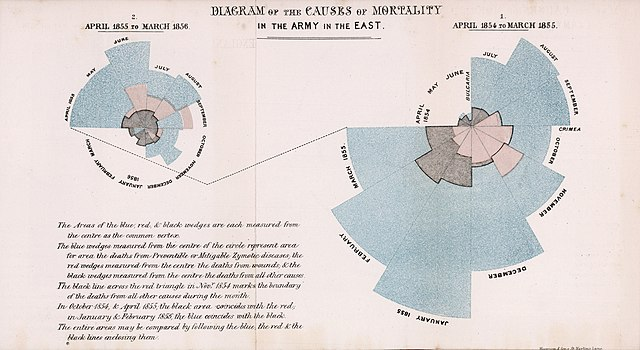
\includegraphics{images/640px-Nightingale-mortality.jpg}

\vspace{2cm}

Este livro/\emph{site} foi iniciado em 2020, durante a pandemia de COVID-19, quando a Universidade Federal Fluminense (UFF) funcionou em regime de ensino remoto durante mais de um ano.

Para atender os alunos do curso de Probabilidade e Estatística do curso de graduação em Ciência da Computação da UFF, decidi gravar aulas em vídeo e disponibilizar os arquivos usados nelas. Foram esses arquivos que deram origem a este livro/\emph{site}.

Este livro/\emph{site} foi construído para pessoas que já saibam programar, embora não necessariamente em R.

Para tirar o máximo proveito deste material, você deve fazer o seguinte:

\begin{enumerate}
\def\labelenumi{\arabic{enumi}.}
\item
  Assistir aos vídeos contidos em cada capítulo. A \emph{playlist} completa está em \url{https://www.youtube.com/playlist?list=PL7SRLwLs7ocaV-Y1vrVU3W7mZnnS0qkWV}.
\item
  Instalar o R no seu computador ou abrir uma conta no RStudio Cloud, para poder usar o R \emph{online}. Você encontra instruções para fazer isto no \protect\hyperlink{rintro}{capítulo de introdução a R}.
\item
  Baixar, \href{https://github.com/fnaufel/probestr}{neste repositório do Github}, o código-fonte deste livro/\emph{site}, para poder rodar e alterar os exemplos.
\item
  Seguir os \emph{links} para outras fontes \emph{online} que abordam assuntos que não são cobertos em detalhes neste curso.
\item
  Fazer os exercícios. Ao longo do tempo, acrescentarei \emph{links} para vídeos explicando as soluções.
\end{enumerate}

\begin{rmdimportant}
{\hl{Se você estiver lendo este material na \emph{web}, você pode clicar nos comandos e funções que aparecem nos blocos de código em R}} para abrir páginas da documentação sobre eles.

Se você preferir ler este livro em pdf, ou se quiser imprimi-lo, \href{https://github.com/fnaufel/probestr/blob/master/docs/probestr.pdf}{faça o \emph{download} do arquivo aqui}.

\end{rmdimportant}

\hypertarget{refrec}{%
\section*{Referências recomendadas}\label{refrec}}
\addcontentsline{toc}{section}{Referências recomendadas}

\hypertarget{em-portuguuxeas}{%
\subsection*{Em português}\label{em-portuguuxeas}}
\addcontentsline{toc}{subsection}{Em português}

\begin{itemize}
\item
  Sillas Gonzaga, \emph{Introdução a R para Visualização e Apresentação de Dados},
  \url{http://sillasgonzaga.com/material/curso_visualizacao/index.html}
\item
  Allan Vieira de Castro Quadros, \emph{Introdução à Análise de Dados em R utilizando Tidyverse}, \url{https://allanvc.github.io/book_IADR-T/}
\item
  Paulo Felipe de Oliveira, Saulo Guerra, Robert McDonnel, \emph{Ciência de Dados com R -- Introdução}, \url{https://cdr.ibpad.com.br/index.html}
\item
  Curso R, \emph{Ciência de Dados em R}, \url{https://livro.curso-r.com/}
\end{itemize}

\hypertarget{em-ingluxeas}{%
\subsection*{Em inglês}\label{em-ingluxeas}}
\addcontentsline{toc}{subsection}{Em inglês}

\begin{itemize}
\item
  Garrett Grolemund, Hadley Wickham, \emph{R for Data Science}, \url{https://r4ds.had.co.nz/}
\item
  Chester Ismay, Albert Y. Kim, \emph{A ModernDive into R and the Tidyverse}, \url{https://moderndive.com/}
\end{itemize}

\hypertarget{exercuxedcio}{%
\section*{Exercício}\label{exercuxedcio}}
\addcontentsline{toc}{section}{Exercício}

\begin{enumerate}
\def\labelenumi{\arabic{enumi}.}
\tightlist
\item
  Pesquise sobre a imagem do início deste capítulo. Ela foi criada em 1858 por Florence Nightingale.
\end{enumerate}

\hypertarget{oque}{%
\chapter{O Que É Estatística?}\label{oque}}

\hypertarget{vuxeddeo-1}{%
\section{Vídeo 1}\label{vuxeddeo-1}}

\begin{center} \url{https://youtu.be/6Q_XSoLCIpc} \end{center}

\hypertarget{exercuxedcios}{%
\section{Exercícios}\label{exercuxedcios}}

\begin{enumerate}
\def\labelenumi{\arabic{enumi}.}
\item
  Você está interessado em estimar a altura de todos os homens da sua faculdade. Para isso, você decide medir as alturas de todos os homens da sua turma de Estatística.

  \begin{itemize}
  \tightlist
  \item
    Qual é a amostra?
  \item
    Qual é a população?
  \end{itemize}
\item
  Um instituto de pesquisa entrevista um grupo de $1000$ pessoas, perguntando a cada uma se ela vai votar a favor do candidato $A$ na próxima eleição. Dos entrevistados, $600$ responderam que sim. A proporção $0{,}6$ (ou $60\%$) é uma estatística ou um parâmetro?
\item
  Você vê alguma diferença entre as cinco situações abaixo? Quais das situações são equivalentes em termos da probabilidade de conseguir $10$ cartas do mesmo naipe?

  \begin{enumerate}
  \def\labelenumii{\alph{enumii}.}
  \item
    Usando um baralho normal, você retira $10$ cartas e registra as cartas retiradas.
  \item
    Usando um baralho normal, você repete a seguinte sequência de ações $10$ vezes: retirar uma carta do baralho, registrar a carta retirada e repor a carta no baralho.
  \item
    Usando uma caixa contendo todas as cartas de $1$ milhão de baralhos reunidos, você retira $10$ cartas e registra as cartas retiradas.
  \item
    Usando uma caixa contendo todas as cartas de $1$ milhão de baralhos reunidos, você repete a seguinte sequência de ações $10$ vezes: retirar uma carta da caixa, registrar a carta retirada e repor a carta na caixa.
  \item
    Usando um baralho \emph{infinito}, você retira $10$ cartas e registra as cartas retiradas.
  \item
    Usando um baralho \emph{infinito}, você repete a seguinte sequência de ações $10$ vezes: retirar uma carta do baralho, registrar a carta retirada e repor a carta no baralho.
  \end{enumerate}
\item
  Qual a graça dos quadrinhos na Figura \ref{fig:xkcd-cor}, que também \href{https://youtu.be/6Q_XSoLCIpc?t=1385}{aparecem no vídeo}?

  \begin{figure}

   {\centering 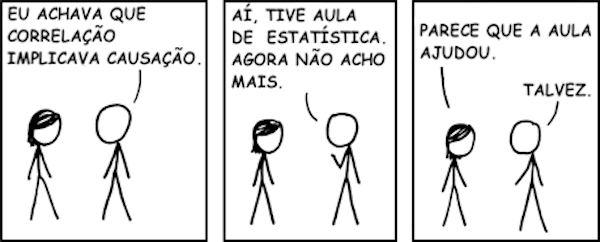
\includegraphics[width=0.9\linewidth]{images/correlation-pt-600} 

   }

   \caption{\url{http://xkcd.com/552/}}\label{fig:xkcd-cor}
   \end{figure}
\item
  Qual a graça dos quadrinhos na Figura \ref{fig:xkcd-blind}?

  \begin{figure}

   {\centering 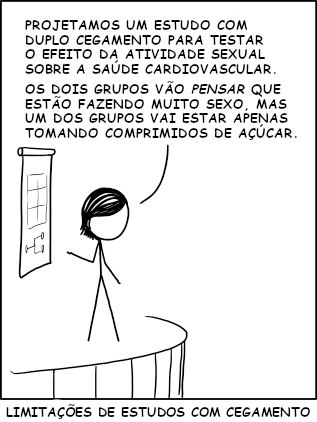
\includegraphics[width=0.5\linewidth]{images/double-blind} 

   }

   \caption{\url{http://xkcd.com/1462/}}\label{fig:xkcd-blind}
   \end{figure}
\item
  Veja este vídeo sobre o cavalo Hans:

  \begin{center} \url{https://youtu.be/G3VkCmdUfZE} \end{center}

  Qual a relação entre esta história e a necessidade de duplo cegamento?
\end{enumerate}





\hypertarget{niveis-de-dados}{%
\section{Vídeo 2}\label{niveis-de-dados}}

\begin{center} \url{https://youtu.be/492VASxlDRo} \end{center}

\hypertarget{exercuxedcios-1}{%
\section{Exercícios}\label{exercuxedcios-1}}

\begin{enumerate}
\def\labelenumi{\arabic{enumi}.}
\item
  Por que não faz sentido calcular a média dos CEPs de um grupo de pessoas?
\item
  Uma temperatura de $-40$ graus Celsius é igual a uma temperatura de $-40$ graus Fahrenheit?
\item
  Uma temperatura de zero graus Celsius é igual a uma temperatura de zero graus Fahrenheit?
\item
  Uma variação de temperatura de $1$ grau Celsius é igual a uma variação de temperatura de $1$ grau Fahrenheit?
\item
  Um saldo bancário de zero reais é igual a um saldo bancário de zero dólares?
\item
  Um produto de $1$ milhão de reais custa o mesmo que um produto de $1$ milhão de dólares?
\item
  Meses representados por números de $1$ a $12$ são dados de que nível?
\end{enumerate}

\hypertarget{rintro}{%
\chapter{Introdução a R}\label{rintro}}

\hypertarget{vuxeddeo-1-1}{%
\section{Vídeo 1}\label{vuxeddeo-1-1}}

\begin{center} \url{https://youtu.be/1kXQDNqm41c} \end{center}

\hypertarget{vuxeddeo-2}{%
\section{Vídeo 2}\label{vuxeddeo-2}}

\begin{center} \url{https://youtu.be/3GEc1oiKDrU} \end{center}

\hypertarget{exercuxedcios-2}{%
\section{Exercícios}\label{exercuxedcios-2}}

\begin{enumerate}
\def\labelenumi{\arabic{enumi}.}
\item
  Para criar sua conta no RStudio Cloud, acesse \url{https://rstudio.cloud/}.
\item
  Se você preferir instalar o R no seu computador, acesse

  \begin{itemize}
  \item
    \url{https://cran.r-project.org/} para baixar e instalar o R, e
  \item
    \url{https://rstudio.com/products/rstudio/download/} para baixar e instalar o RStudio, um IDE específico para R.
  \end{itemize}
\item
  Abra o RStudio Cloud ou o seu RStudio instalado localmente.
\item
  Crie um novo projeto. {\hl{Sempre trabalhe em projetos para ter seus arquivos organizados.}}
\item
  Para instalar o \href{https://swirlstats.com/}{\texttt{swirl} (pacote do R para exercícios interativos)}, execute o seguinte comando no console do RStudio:

\begin{Shaded}
\begin{Highlighting}[]
\FunctionTok{install.packages}\NormalTok{(}\StringTok{"swirl"}\NormalTok{)}
\end{Highlighting}
\end{Shaded}
\item
  Para instalar os exercícios de introdução a R, execute os seguintes comandos no console do RStudio:

\begin{Shaded}
\begin{Highlighting}[]
\FunctionTok{library}\NormalTok{(swirl)}
\FunctionTok{install\_course\_github}\NormalTok{(}\StringTok{\textquotesingle{}fnaufel\textquotesingle{}}\NormalTok{, }\StringTok{\textquotesingle{}introR\textquotesingle{}}\NormalTok{)}
\end{Highlighting}
\end{Shaded}
\item
  Mude o idioma para português e execute o \texttt{swirl}.

\begin{Shaded}
\begin{Highlighting}[]
\FunctionTok{select\_language}\NormalTok{(}\StringTok{\textquotesingle{}portuguese\textquotesingle{}}\NormalTok{, }\AttributeTok{append\_rprofile =} \ConstantTok{TRUE}\NormalTok{)}
\FunctionTok{swirl}\NormalTok{()}
\end{Highlighting}
\end{Shaded}
\item
  Na primeira execução, você vai precisar se identificar (qualquer nome serve). Com essa identificação, o \texttt{swirl} vai registrar o seu progresso nas lições.
\item
  No \texttt{swirl}, as perguntas são mostradas no console. Você também deve responder no console.
\item
  Às vezes, um \emph{script} será aberto no editor de textos para que você complete um programa. Quando seu programa estiver pronto, salve o arquivo e digite \texttt{submit()} no console para o \texttt{swirl} processar o \emph{script}.
\item
  O \texttt{swirl} dá instruções claras no console. Na dúvida, digite \texttt{info()} no \emph{prompt} do R (\texttt{\textgreater{}}).
\item
  Se, em vez do \emph{prompt} do R, o console mostrar reticências (\texttt{...}), tecle \emph{Enter}.
\item
  Se nada funcionar, tecle \emph{ESC}.
\item
  Para sair do \texttt{swirl()}, digite \texttt{bye()} no \emph{prompt} do R.
\item
  Para voltar para os exercícios, digite

\begin{Shaded}
\begin{Highlighting}[]
\FunctionTok{library}\NormalTok{(swirl)}
\FunctionTok{swirl}\NormalTok{()}
\end{Highlighting}
\end{Shaded}
\end{enumerate}

\hypertarget{introduuxe7uxe3o-ao-tidyverse}{%
\chapter{\texorpdfstring{Introdução ao \texttt{tidyverse}}{Introdução ao tidyverse}}\label{introduuxe7uxe3o-ao-tidyverse}}

\begin{rmdtip}
Busque mais informações sobre os pacotes que compõem o \texttt{tidyverse} \protect\hyperlink{refrec}{nas referências recomendadas}.

\end{rmdtip}

\hypertarget{criando-uma-tibble}{%
\section{\texorpdfstring{Criando uma \emph{tibble}}{Criando uma tibble}}\label{criando-uma-tibble}}

\begin{itemize}
\item
  Uma \emph{tibble} é uma tabela retangular.
\item
  {\hl{Cada coluna é um vetor}}:

\begin{Shaded}
\begin{Highlighting}[]
\NormalTok{cores }\OtherTok{\textless{}{-}} \FunctionTok{tibble}\NormalTok{(}
  \AttributeTok{pessoa =} \FunctionTok{c}\NormalTok{(}\StringTok{\textquotesingle{}João\textquotesingle{}}\NormalTok{, }\StringTok{\textquotesingle{}Maria\textquotesingle{}}\NormalTok{, }\StringTok{\textquotesingle{}Pedro\textquotesingle{}}\NormalTok{, }\StringTok{\textquotesingle{}Ana\textquotesingle{}}\NormalTok{),}
  \StringTok{\textquotesingle{}cor favorita\textquotesingle{}} \OtherTok{=} \FunctionTok{c}\NormalTok{(}\StringTok{\textquotesingle{}azul\textquotesingle{}}\NormalTok{, }\StringTok{\textquotesingle{}rosa\textquotesingle{}}\NormalTok{, }\StringTok{\textquotesingle{}preto\textquotesingle{}}\NormalTok{, }\StringTok{\textquotesingle{}branco\textquotesingle{}}\NormalTok{)}
\NormalTok{)}

\NormalTok{cores}
\end{Highlighting}
\end{Shaded}

\begin{verbatim}
## # A tibble: 4 x 2
##   pessoa `cor favorita`
##   <chr>  <chr>         
## 1 João   azul          
## 2 Maria  rosa          
## 3 Pedro  preto         
## 4 Ana    branco
\end{verbatim}
\item
  Isto é um pouco diferente da maneira como estamos acostumados a ver tabelas (como uma coleção de linhas, em vez de uma coleção de colunas).
\item
  A função \texttt{tribble} permite a entrada de forma mais natural, linha a linha. {\hl{Lembre-se de usar {\mbox{\texttt{\textasciitilde{}}}} antes dos nomes das colunas.}}

\begin{Shaded}
\begin{Highlighting}[]
\NormalTok{cores }\OtherTok{\textless{}{-}} \FunctionTok{tribble}\NormalTok{(}
  \SpecialCharTok{\textasciitilde{}}\NormalTok{pessoa, }\SpecialCharTok{\textasciitilde{}}\StringTok{\textquotesingle{}cor favorita\textquotesingle{}}\NormalTok{,}
   \StringTok{"João"}\NormalTok{,          }\StringTok{"azul"}\NormalTok{,}
  \StringTok{"Maria"}\NormalTok{,          }\StringTok{"rosa"}\NormalTok{,}
  \StringTok{"Pedro"}\NormalTok{,         }\StringTok{"preto"}\NormalTok{,}
    \StringTok{"Ana"}\NormalTok{,        }\StringTok{"branco"}
\NormalTok{)}

\NormalTok{cores}
\end{Highlighting}
\end{Shaded}

\begin{verbatim}
## # A tibble: 4 x 2
##   pessoa `cor favorita`
##   <chr>  <chr>         
## 1 João   azul          
## 2 Maria  rosa          
## 3 Pedro  preto         
## 4 Ana    branco
\end{verbatim}

  \begin{rmdcaution}
  Mesmo que você crie uma \emph{tibble} linha a linha, o R vai continuar tratando sua \emph{tibble} como uma coleção de colunas.

  É importante lembrar disto para entender a forma como R manipula estas tabelas.

  \end{rmdcaution}
\item
  Se uma coluna não puder ser armazenada em um vetor, a coluna será uma lista (com vetores como elementos):

\begin{Shaded}
\begin{Highlighting}[]
\NormalTok{cores }\OtherTok{\textless{}{-}} \FunctionTok{tibble}\NormalTok{(}
  \AttributeTok{pessoa =} \FunctionTok{c}\NormalTok{(}\StringTok{\textquotesingle{}João\textquotesingle{}}\NormalTok{, }\StringTok{\textquotesingle{}Maria\textquotesingle{}}\NormalTok{, }\StringTok{\textquotesingle{}Pedro\textquotesingle{}}\NormalTok{, }\StringTok{\textquotesingle{}Ana\textquotesingle{}}\NormalTok{),}
  \StringTok{\textquotesingle{}cor favorita\textquotesingle{}} \OtherTok{=} \FunctionTok{list}\NormalTok{(}
    \FunctionTok{c}\NormalTok{(}\StringTok{\textquotesingle{}azul\textquotesingle{}}\NormalTok{, }\StringTok{\textquotesingle{}roxo\textquotesingle{}}\NormalTok{),}
    \FunctionTok{c}\NormalTok{(}\StringTok{\textquotesingle{}rosa\textquotesingle{}}\NormalTok{, }\StringTok{\textquotesingle{}magenta\textquotesingle{}}\NormalTok{),}
    \ConstantTok{NA}\NormalTok{,}
    \StringTok{\textquotesingle{}branco\textquotesingle{}}
\NormalTok{  )}
\NormalTok{)}

\NormalTok{cores}
\end{Highlighting}
\end{Shaded}

\begin{verbatim}
## # A tibble: 4 x 2
##   pessoa `cor favorita`
##   <chr>  <list>        
## 1 João   <chr [2]>     
## 2 Maria  <chr [2]>     
## 3 Pedro  <lgl [1]>     
## 4 Ana    <chr [1]>
\end{verbatim}
\item
  Use \texttt{View()} para examinar interativamente o conteúdo de uma coluna-lista:

\begin{Shaded}
\begin{Highlighting}[]
\NormalTok{cores }\SpecialCharTok{\%\textgreater{}\%} \FunctionTok{View}\NormalTok{()}
\end{Highlighting}
\end{Shaded}
\end{itemize}

\hypertarget{operador-de-pipe}{%
\section{\texorpdfstring{Operador de \emph{pipe} (\texttt{\%\textgreater{}\%})}{Operador de pipe (\%\textgreater\%)}}\label{operador-de-pipe}}

\begin{itemize}
\tightlist
\item
  O \texttt{tidyverse} inclui o pacote \texttt{magrittr}, que contém o operador \texttt{\%\textgreater{}\%}, chamado \emph{pipe}.\footnote{Por que o nome do pacote e o nome do operador formam um trocadilho?}
\end{itemize}

\begin{itemize}
\item
  A idéia é facilitar a leitura de {\hl{composições de funções}}. O código

\begin{Shaded}
\begin{Highlighting}[]
\NormalTok{y }\OtherTok{\textless{}{-}} \FunctionTok{h}\NormalTok{(}\FunctionTok{g}\NormalTok{(}\FunctionTok{f}\NormalTok{(x)))}
\end{Highlighting}
\end{Shaded}

  pode ser escrito como

\begin{Shaded}
\begin{Highlighting}[]
\NormalTok{y }\OtherTok{\textless{}{-}}\NormalTok{ x }\SpecialCharTok{\%\textgreater{}\%} \FunctionTok{f}\NormalTok{() }\SpecialCharTok{\%\textgreater{}\%} \FunctionTok{g}\NormalTok{() }\SpecialCharTok{\%\textgreater{}\%} \FunctionTok{h}\NormalTok{()}
\end{Highlighting}
\end{Shaded}
\item
  Esta segunda versão é mais fiel à ordem em que as operações acontecem.
\item
  Na verdade, R tem um operador de {\hl{atribuição para a direita}}, mas poucas pessoas recomendam usá-lo:

\begin{Shaded}
\begin{Highlighting}[]
\NormalTok{x }\SpecialCharTok{\%\textgreater{}\%} \FunctionTok{f}\NormalTok{() }\SpecialCharTok{\%\textgreater{}\%} \FunctionTok{g}\NormalTok{() }\SpecialCharTok{\%\textgreater{}\%} \FunctionTok{h}\NormalTok{() }\OtherTok{{-}\textgreater{}}\NormalTok{ y}
\end{Highlighting}
\end{Shaded}
\item
  Se \texttt{f}, \texttt{g} e \texttt{h} forem funções de um argumento só, os parênteses podem ser omitidos:

\begin{Shaded}
\begin{Highlighting}[]
\NormalTok{y }\OtherTok{\textless{}{-}}\NormalTok{ x }\SpecialCharTok{\%\textgreater{}\%}\NormalTok{ f }\SpecialCharTok{\%\textgreater{}\%}\NormalTok{ g }\SpecialCharTok{\%\textgreater{}\%}\NormalTok{ h}
\end{Highlighting}
\end{Shaded}
\item
  Se a função \texttt{f} tiver outros argumentos, escreva-os normalmente na chamada a \texttt{f}:

\begin{Shaded}
\begin{Highlighting}[]
\NormalTok{y }\OtherTok{\textless{}{-}}\NormalTok{ x }\SpecialCharTok{\%\textgreater{}\%} \FunctionTok{mean}\NormalTok{(}\AttributeTok{na.rm =} \ConstantTok{TRUE}\NormalTok{)}
\end{Highlighting}
\end{Shaded}
\item
  O \emph{pipe} \texttt{EXP\ \%\textgreater{}\%\ f(...)} sempre insere o resultado da expressão \texttt{EXP} como o {\hl{primeiro argumento da função {\mbox{\texttt{f}}}}}.
\item
  Se você precisar que o resultado da expressão \texttt{EXP} seja inserido em outra posição na lista de argumentos de \texttt{f}, use um ponto ``\texttt{.}'' para isso:

\begin{Shaded}
\begin{Highlighting}[]
\NormalTok{x }\SpecialCharTok{\%\textgreater{}\%} \FunctionTok{consultar}\NormalTok{(df, .)}
\end{Highlighting}
\end{Shaded}

  equivale a

\begin{Shaded}
\begin{Highlighting}[]
\FunctionTok{consultar}\NormalTok{(df, x)}
\end{Highlighting}
\end{Shaded}
\end{itemize}

\hypertarget{formato-tidy}{%
\section{\texorpdfstring{Formato \emph{tidy}}{Formato tidy}}\label{formato-tidy}}

\begin{itemize}
\item
  Nossa última versão da \emph{tibble} \texttt{cores} é um pouco mais complexa do que deveria ser:

\begin{Shaded}
\begin{Highlighting}[]
\NormalTok{cores}
\end{Highlighting}
\end{Shaded}

\begin{verbatim}
## # A tibble: 4 x 2
##   pessoa `cor favorita`
##   <chr>  <list>        
## 1 João   <chr [2]>     
## 2 Maria  <chr [2]>     
## 3 Pedro  <lgl [1]>     
## 4 Ana    <chr [1]>
\end{verbatim}
\item
  O formato \emph{tidy} exige que

  \begin{enumerate}
  \def\labelenumi{\arabic{enumi}.}
  \item
    {\hl{Cada linha}} da \emph{tibble} corresponda a uma {\hl{observação}} sobre um indivíduo,
  \item
    {\hl{Cada coluna}} corresponda a {\hl{uma variável observada}}, e
  \item
    {\hl{Cada célula}} contenha {\hl{um valor}} da variável.
  \end{enumerate}
\item
  Na \emph{tibble} \texttt{cores}, a primeira e a segunda exigências são satisfeitas, mas a terceira não, pois algumas células contém valores múltiplos.
\item
  A \emph{tibble} não está no formato \emph{tidy}.
\item
  Podemos ``extrair'' estes vetores ``aninhados'' usando o comando \texttt{unnest}, do pacote \texttt{tidyr}:

\begin{Shaded}
\begin{Highlighting}[]
\NormalTok{cores }\OtherTok{\textless{}{-}}\NormalTok{ cores }\SpecialCharTok{\%\textgreater{}\%} 
  \FunctionTok{unnest}\NormalTok{(}\StringTok{\textasciigrave{}}\AttributeTok{cor favorita}\StringTok{\textasciigrave{}}\NormalTok{)}

\NormalTok{cores}
\end{Highlighting}
\end{Shaded}

\begin{verbatim}
## # A tibble: 6 x 2
##   pessoa `cor favorita`
##   <chr>  <chr>         
## 1 João   azul          
## 2 João   roxo          
## 3 Maria  rosa          
## 4 Maria  magenta       
## 5 Pedro  <NA>          
## 6 Ana    branco
\end{verbatim}
\item
  {\hl{A maioria das funções do {\mbox{\texttt{tidyverse}}} exige que as \emph{tibbles} estejam neste formato \emph{tidy}.}}
\item
  Um exemplo mais complexo é o \emph{dataset} \texttt{billboard}, com as seguintes colunas (para cada música que estava no \emph{top 100} da Billboard no ano de $2000$):

  \begin{itemize}
  \item
    Nome do artista ou banda;
  \item
    Nome da música;
  \item
    Data em que a música entrou no \emph{top 100} da Billboard;
  \item
    Para cada uma das $76$ semanas seguintes, a posição da música no \emph{top 100}.
  \end{itemize}

\begin{Shaded}
\begin{Highlighting}[]
\NormalTok{billboard }\SpecialCharTok{\%\textgreater{}\%} \FunctionTok{glimpse}\NormalTok{()}
\end{Highlighting}
\end{Shaded}

\begin{verbatim}
## Rows: 317
## Columns: 79
## $ artist       <chr> "2 Pac", "2Ge+her", "3 Doors Down", "3 Doors Dow~
## $ track        <chr> "Baby Don't Cry (Keep...", "The Hardest Part Of ~
## $ date.entered <date> 2000-02-26, 2000-09-02, 2000-04-08, 2000-10-21,~
## $ wk1          <dbl> 87, 91, 81, 76, 57, 51, 97, 84, 59, 76, 84, 57, ~
## $ wk2          <dbl> 82, 87, 70, 76, 34, 39, 97, 62, 53, 76, 84, 47, ~
## $ wk3          <dbl> 72, 92, 68, 72, 25, 34, 96, 51, 38, 74, 75, 45, ~
## $ wk4          <dbl> 77, NA, 67, 69, 17, 26, 95, 41, 28, 69, 73, 29, ~
## $ wk5          <dbl> 87, NA, 66, 67, 17, 26, 100, 38, 21, 68, 73, 23,~
## $ wk6          <dbl> 94, NA, 57, 65, 31, 19, NA, 35, 18, 67, 69, 18, ~
## $ wk7          <dbl> 99, NA, 54, 55, 36, 2, NA, 35, 16, 61, 68, 11, 2~
## $ wk8          <dbl> NA, NA, 53, 59, 49, 2, NA, 38, 14, 58, 65, 9, 17~
## $ wk9          <dbl> NA, NA, 51, 62, 53, 3, NA, 38, 12, 57, 73, 9, 17~
## $ wk10         <dbl> NA, NA, 51, 61, 57, 6, NA, 36, 10, 59, 83, 11, 1~
## $ wk11         <dbl> NA, NA, 51, 61, 64, 7, NA, 37, 9, 66, 92, 1, 17,~
## $ wk12         <dbl> NA, NA, 51, 59, 70, 22, NA, 37, 8, 68, NA, 1, 3,~
## $ wk13         <dbl> NA, NA, 47, 61, 75, 29, NA, 38, 6, 61, NA, 1, 3,~
## $ wk14         <dbl> NA, NA, 44, 66, 76, 36, NA, 49, 1, 67, NA, 1, 7,~
## $ wk15         <dbl> NA, NA, 38, 72, 78, 47, NA, 61, 2, 59, NA, 4, 10~
## $ wk16         <dbl> NA, NA, 28, 76, 85, 67, NA, 63, 2, 63, NA, 8, 17~
## $ wk17         <dbl> NA, NA, 22, 75, 92, 66, NA, 62, 2, 67, NA, 12, 2~
## $ wk18         <dbl> NA, NA, 18, 67, 96, 84, NA, 67, 2, 71, NA, 22, 2~
## $ wk19         <dbl> NA, NA, 18, 73, NA, 93, NA, 83, 3, 79, NA, 23, 2~
## $ wk20         <dbl> NA, NA, 14, 70, NA, 94, NA, 86, 4, 89, NA, 43, 4~
## $ wk21         <dbl> NA, NA, 12, NA, NA, NA, NA, NA, 5, NA, NA, 44, 4~
## $ wk22         <dbl> NA, NA, 7, NA, NA, NA, NA, NA, 5, NA, NA, NA, 50~
## $ wk23         <dbl> NA, NA, 6, NA, NA, NA, NA, NA, 6, NA, NA, NA, NA~
## $ wk24         <dbl> NA, NA, 6, NA, NA, NA, NA, NA, 9, NA, NA, NA, NA~
## $ wk25         <dbl> NA, NA, 6, NA, NA, NA, NA, NA, 13, NA, NA, NA, N~
## $ wk26         <dbl> NA, NA, 5, NA, NA, NA, NA, NA, 14, NA, NA, NA, N~
## $ wk27         <dbl> NA, NA, 5, NA, NA, NA, NA, NA, 16, NA, NA, NA, N~
## $ wk28         <dbl> NA, NA, 4, NA, NA, NA, NA, NA, 23, NA, NA, NA, N~
## $ wk29         <dbl> NA, NA, 4, NA, NA, NA, NA, NA, 22, NA, NA, NA, N~
## $ wk30         <dbl> NA, NA, 4, NA, NA, NA, NA, NA, 33, NA, NA, NA, N~
## $ wk31         <dbl> NA, NA, 4, NA, NA, NA, NA, NA, 36, NA, NA, NA, N~
## $ wk32         <dbl> NA, NA, 3, NA, NA, NA, NA, NA, 43, NA, NA, NA, N~
## $ wk33         <dbl> NA, NA, 3, NA, NA, NA, NA, NA, NA, NA, NA, NA, N~
## $ wk34         <dbl> NA, NA, 3, NA, NA, NA, NA, NA, NA, NA, NA, NA, N~
## $ wk35         <dbl> NA, NA, 4, NA, NA, NA, NA, NA, NA, NA, NA, NA, N~
## $ wk36         <dbl> NA, NA, 5, NA, NA, NA, NA, NA, NA, NA, NA, NA, N~
## $ wk37         <dbl> NA, NA, 5, NA, NA, NA, NA, NA, NA, NA, NA, NA, N~
## $ wk38         <dbl> NA, NA, 9, NA, NA, NA, NA, NA, NA, NA, NA, NA, N~
## $ wk39         <dbl> NA, NA, 9, NA, NA, NA, NA, NA, NA, NA, NA, NA, N~
## $ wk40         <dbl> NA, NA, 15, NA, NA, NA, NA, NA, NA, NA, NA, NA, ~
## $ wk41         <dbl> NA, NA, 14, NA, NA, NA, NA, NA, NA, NA, NA, NA, ~
## $ wk42         <dbl> NA, NA, 13, NA, NA, NA, NA, NA, NA, NA, NA, NA, ~
## $ wk43         <dbl> NA, NA, 14, NA, NA, NA, NA, NA, NA, NA, NA, NA, ~
## $ wk44         <dbl> NA, NA, 16, NA, NA, NA, NA, NA, NA, NA, NA, NA, ~
## $ wk45         <dbl> NA, NA, 17, NA, NA, NA, NA, NA, NA, NA, NA, NA, ~
## $ wk46         <dbl> NA, NA, 21, NA, NA, NA, NA, NA, NA, NA, NA, NA, ~
## $ wk47         <dbl> NA, NA, 22, NA, NA, NA, NA, NA, NA, NA, NA, NA, ~
## $ wk48         <dbl> NA, NA, 24, NA, NA, NA, NA, NA, NA, NA, NA, NA, ~
## $ wk49         <dbl> NA, NA, 28, NA, NA, NA, NA, NA, NA, NA, NA, NA, ~
## $ wk50         <dbl> NA, NA, 33, NA, NA, NA, NA, NA, NA, NA, NA, NA, ~
## $ wk51         <dbl> NA, NA, 42, NA, NA, NA, NA, NA, NA, NA, NA, NA, ~
## $ wk52         <dbl> NA, NA, 42, NA, NA, NA, NA, NA, NA, NA, NA, NA, ~
## $ wk53         <dbl> NA, NA, 49, NA, NA, NA, NA, NA, NA, NA, NA, NA, ~
## $ wk54         <dbl> NA, NA, NA, NA, NA, NA, NA, NA, NA, NA, NA, NA, ~
## $ wk55         <dbl> NA, NA, NA, NA, NA, NA, NA, NA, NA, NA, NA, NA, ~
## $ wk56         <dbl> NA, NA, NA, NA, NA, NA, NA, NA, NA, NA, NA, NA, ~
## $ wk57         <dbl> NA, NA, NA, NA, NA, NA, NA, NA, NA, NA, NA, NA, ~
## $ wk58         <dbl> NA, NA, NA, NA, NA, NA, NA, NA, NA, NA, NA, NA, ~
## $ wk59         <dbl> NA, NA, NA, NA, NA, NA, NA, NA, NA, NA, NA, NA, ~
## $ wk60         <dbl> NA, NA, NA, NA, NA, NA, NA, NA, NA, NA, NA, NA, ~
## $ wk61         <dbl> NA, NA, NA, NA, NA, NA, NA, NA, NA, NA, NA, NA, ~
## $ wk62         <dbl> NA, NA, NA, NA, NA, NA, NA, NA, NA, NA, NA, NA, ~
## $ wk63         <dbl> NA, NA, NA, NA, NA, NA, NA, NA, NA, NA, NA, NA, ~
## $ wk64         <dbl> NA, NA, NA, NA, NA, NA, NA, NA, NA, NA, NA, NA, ~
## $ wk65         <dbl> NA, NA, NA, NA, NA, NA, NA, NA, NA, NA, NA, NA, ~
## $ wk66         <lgl> NA, NA, NA, NA, NA, NA, NA, NA, NA, NA, NA, NA, ~
## $ wk67         <lgl> NA, NA, NA, NA, NA, NA, NA, NA, NA, NA, NA, NA, ~
## $ wk68         <lgl> NA, NA, NA, NA, NA, NA, NA, NA, NA, NA, NA, NA, ~
## $ wk69         <lgl> NA, NA, NA, NA, NA, NA, NA, NA, NA, NA, NA, NA, ~
## $ wk70         <lgl> NA, NA, NA, NA, NA, NA, NA, NA, NA, NA, NA, NA, ~
## $ wk71         <lgl> NA, NA, NA, NA, NA, NA, NA, NA, NA, NA, NA, NA, ~
## $ wk72         <lgl> NA, NA, NA, NA, NA, NA, NA, NA, NA, NA, NA, NA, ~
## $ wk73         <lgl> NA, NA, NA, NA, NA, NA, NA, NA, NA, NA, NA, NA, ~
## $ wk74         <lgl> NA, NA, NA, NA, NA, NA, NA, NA, NA, NA, NA, NA, ~
## $ wk75         <lgl> NA, NA, NA, NA, NA, NA, NA, NA, NA, NA, NA, NA, ~
## $ wk76         <lgl> NA, NA, NA, NA, NA, NA, NA, NA, NA, NA, NA, NA, ~
\end{verbatim}
\item
  Vamos renomear as colunas:

\begin{Shaded}
\begin{Highlighting}[]
\NormalTok{bb }\OtherTok{\textless{}{-}}\NormalTok{ billboard }\SpecialCharTok{\%\textgreater{}\%} 
  \FunctionTok{rename}\NormalTok{(}
    \AttributeTok{artista =}\NormalTok{ artist,}
    \AttributeTok{musica =}\NormalTok{ track,}
    \AttributeTok{entrou =}\NormalTok{ date.entered}
\NormalTok{  )}
\end{Highlighting}
\end{Shaded}

\begin{Shaded}
\begin{Highlighting}[]
\NormalTok{bb }\SpecialCharTok{\%\textgreater{}\%} \FunctionTok{head}\NormalTok{()}
\end{Highlighting}
\end{Shaded}

\begin{verbatim}
## # A tibble: 6 x 79
##   artista   musica entrou       wk1   wk2   wk3   wk4   wk5   wk6   wk7
##   <chr>     <chr>  <date>     <dbl> <dbl> <dbl> <dbl> <dbl> <dbl> <dbl>
## 1 2 Pac     Baby ~ 2000-02-26    87    82    72    77    87    94    99
## 2 2Ge+her   The H~ 2000-09-02    91    87    92    NA    NA    NA    NA
## 3 3 Doors ~ Krypt~ 2000-04-08    81    70    68    67    66    57    54
## 4 3 Doors ~ Loser  2000-10-21    76    76    72    69    67    65    55
## 5 504 Boyz  Wobbl~ 2000-04-15    57    34    25    17    17    31    36
## 6 98^0      Give ~ 2000-08-19    51    39    34    26    26    19     2
## # ... with 69 more variables: wk8 <dbl>, wk9 <dbl>, wk10 <dbl>,
## #   wk11 <dbl>, wk12 <dbl>, wk13 <dbl>, wk14 <dbl>, wk15 <dbl>,
## #   wk16 <dbl>, wk17 <dbl>, wk18 <dbl>, wk19 <dbl>, wk20 <dbl>,
## #   wk21 <dbl>, wk22 <dbl>, wk23 <dbl>, wk24 <dbl>, wk25 <dbl>,
## #   wk26 <dbl>, wk27 <dbl>, wk28 <dbl>, wk29 <dbl>, wk30 <dbl>,
## #   wk31 <dbl>, wk32 <dbl>, wk33 <dbl>, wk34 <dbl>, wk35 <dbl>,
## #   wk36 <dbl>, wk37 <dbl>, wk38 <dbl>, wk39 <dbl>, wk40 <dbl>, ...
\end{verbatim}
\item
  {\hl{O que é uma observação}} neste conjunto de dados?

  {\hl{A posição, em uma semana, de uma música}} que esteve no \emph{top} $100$ da \emph{Billboard} durante o ano \emph{2000}.
\item
  {\hl{Quais são as variáveis}} que qualificam cada observação?

  \begin{itemize}
  \item
    O artista,
  \item
    O título da música,
  \item
    A posiçao da música no \emph{top} $100$ da \emph{Billboard} em cada uma das $76$ semanas depois que ela entrou na lista.
  \end{itemize}
\item
  Este último item é complexo, e o criador da \emph{tibble} decidiu criar uma coluna por semana.
\item
  {\hl{Uma decisão ruim, pois existe informação embutida nos nomes das colunas.}} A coluna \texttt{wk68} corresponde à posição da música na semana $68$ após ela entrar na lista, {\hl{mas o número da semana só aparece no nome da coluna}}!
\item
  Isto {\hl{nunca}} deve acontecer. {\hl{A informação deve sempre estar nas células.}}
\item
  Vamos simplificar as coisas criando duas colunas:

  \begin{itemize}
  \item
    \texttt{semana}, com o número da semana; perceba que esta informação vem dos nomes das colunas,
  \item
    \texttt{pos}, com a posição da música naquela semana; esta informação vem das células.
  \end{itemize}
\item
  A \emph{tibble}, que antes era larga, {\hl{vai ser mais estreita e mais longa}}.
\item
  A função \texttt{pivot\_longer}, do pacote \texttt{tidyr}, vai fazer o trabalho --- inclusive extraindo os números das semanas dos nomes das colunas:

\begin{Shaded}
\begin{Highlighting}[]
\NormalTok{bb\_tidy }\OtherTok{\textless{}{-}}\NormalTok{ bb }\SpecialCharTok{\%\textgreater{}\%} 
  \FunctionTok{pivot\_longer}\NormalTok{(}
\NormalTok{    wk1}\SpecialCharTok{:}\NormalTok{wk76,}
    \AttributeTok{names\_to =} \StringTok{\textquotesingle{}semana\textquotesingle{}}\NormalTok{,}
    \AttributeTok{names\_prefix =} \StringTok{\textquotesingle{}wk\textquotesingle{}}\NormalTok{,}
    \AttributeTok{names\_transform =} \FunctionTok{list}\NormalTok{(}
      \AttributeTok{semana =}\NormalTok{ as.integer}
\NormalTok{    ),}
    \AttributeTok{values\_to =} \StringTok{\textquotesingle{}pos\textquotesingle{}}
\NormalTok{  )}

\NormalTok{bb\_tidy}
\end{Highlighting}
\end{Shaded}

\begin{verbatim}
## # A tibble: 24.092 x 5
##   artista musica                  entrou     semana   pos
##   <chr>   <chr>                   <date>      <int> <dbl>
## 1 2 Pac   Baby Don't Cry (Keep... 2000-02-26      1    87
## 2 2 Pac   Baby Don't Cry (Keep... 2000-02-26      2    82
## 3 2 Pac   Baby Don't Cry (Keep... 2000-02-26      3    72
## 4 2 Pac   Baby Don't Cry (Keep... 2000-02-26      4    77
## 5 2 Pac   Baby Don't Cry (Keep... 2000-02-26      5    87
## 6 2 Pac   Baby Don't Cry (Keep... 2000-02-26      6    94
## # ... with 24.086 more rows
\end{verbatim}
\item
  O R só mostra, por \emph{default}, as $1000$ primeiras linhas de uma \emph{tibble}.
\item
  Na verdade, o número de linhas da tabela original era

\begin{Shaded}
\begin{Highlighting}[]
\NormalTok{bb }\SpecialCharTok{\%\textgreater{}\%} \FunctionTok{nrow}\NormalTok{()}
\end{Highlighting}
\end{Shaded}

\begin{verbatim}
## [1] 317
\end{verbatim}
\item
  O número de linhas, depois de \texttt{pivot\_longer}, ficou:

\begin{Shaded}
\begin{Highlighting}[]
\NormalTok{bb\_tidy }\SpecialCharTok{\%\textgreater{}\%} \FunctionTok{nrow}\NormalTok{()}
\end{Highlighting}
\end{Shaded}

\begin{verbatim}
## [1] 24092
\end{verbatim}
\item
  Existem linhas onde \texttt{pos} tem o valor \texttt{NA}. São resultado da organização original dos dados, onde o \texttt{NA} indicava que a música não estava no \emph{top} $100$ naquela semana.
\item
  No novo formato, a ausência da linha com aquele número de semana já basta para indicar isto. Então, vamos eliminar as linhas onde \texttt{pos} é \texttt{NA}.
\item
  A função \texttt{filter} {\hl{mantém}} as linhas que {\hl{satisfazem}} a condição dada; por isso, a condição é ``\texttt{pos} não é \texttt{NA}'':

\begin{Shaded}
\begin{Highlighting}[]
\NormalTok{bb\_tidy }\OtherTok{\textless{}{-}}\NormalTok{ bb\_tidy }\SpecialCharTok{\%\textgreater{}\%} 
  \FunctionTok{filter}\NormalTok{(}\SpecialCharTok{!}\FunctionTok{is.na}\NormalTok{(pos))}

\NormalTok{bb\_tidy}
\end{Highlighting}
\end{Shaded}

\begin{verbatim}
## # A tibble: 5.307 x 5
##   artista musica                  entrou     semana   pos
##   <chr>   <chr>                   <date>      <int> <dbl>
## 1 2 Pac   Baby Don't Cry (Keep... 2000-02-26      1    87
## 2 2 Pac   Baby Don't Cry (Keep... 2000-02-26      2    82
## 3 2 Pac   Baby Don't Cry (Keep... 2000-02-26      3    72
## 4 2 Pac   Baby Don't Cry (Keep... 2000-02-26      4    77
## 5 2 Pac   Baby Don't Cry (Keep... 2000-02-26      5    87
## 6 2 Pac   Baby Don't Cry (Keep... 2000-02-26      6    94
## # ... with 5.301 more rows
\end{verbatim}
\item
  O número de linhas ficou

\begin{Shaded}
\begin{Highlighting}[]
\NormalTok{bb\_tidy }\SpecialCharTok{\%\textgreater{}\%} \FunctionTok{nrow}\NormalTok{()}
\end{Highlighting}
\end{Shaded}

\begin{verbatim}
## [1] 5307
\end{verbatim}
\end{itemize}

\hypertarget{exercuxedcios-3}{%
\subsection{Exercícios}\label{exercuxedcios-3}}

\begin{itemize}
\item
  Todas as semanas deste conjunto de dados são do ano $2000$?
\item
  Qual é o tipo do {\hl{primeiro}} argumento da função \texttt{filter()}?
\end{itemize}

\hypertarget{manipulando-os-dados}{%
\section{Manipulando os dados}\label{manipulando-os-dados}}

\hypertarget{criando-novas-colunas-mutate-transmute}{%
\subsection{\texorpdfstring{Criando novas colunas: \texttt{mutate}, \texttt{transmute}}{Criando novas colunas: mutate, transmute}}\label{criando-novas-colunas-mutate-transmute}}

\begin{itemize}
\item
  O \emph{data frame}\footnote{Considere \emph{data frame} como sinônimo de \emph{tibble}. Na verdade, \emph{tibbles} formam um superconjunto de \emph{data frames}: todo \emph{data frame} é uma \emph{tibble}, mas nem toda \emph{tibble} é um \emph{data frame}.} \texttt{cars} tem dados (de $1920$!) sobre as distâncias de frenagem (em pés) de um carro viajando a diversas velocidades (em milhas por hora):

\begin{Shaded}
\begin{Highlighting}[]
\NormalTok{cars}
\end{Highlighting}
\end{Shaded}

\begin{verbatim}
## # A tibble: 50 x 2
##   speed  dist
##   <dbl> <dbl>
## 1     4     2
## 2     4    10
## 3     7     4
## 4     7    22
## 5     8    16
## 6     9    10
## # ... with 44 more rows
\end{verbatim}
\item
  Vamos criar colunas novas com os valores convertidos para km/h e metros; além disso, uma coluna com a taxa de frenagem:

\begin{Shaded}
\begin{Highlighting}[]
\NormalTok{cars }\SpecialCharTok{\%\textgreater{}\%} 
  \FunctionTok{mutate}\NormalTok{(}
    \AttributeTok{velocidade =}\NormalTok{ speed }\SpecialCharTok{*} \FloatTok{1.6}\NormalTok{,}
    \AttributeTok{distancia =}\NormalTok{ dist }\SpecialCharTok{*}\NormalTok{ .}\DecValTok{33}\NormalTok{,}
    \AttributeTok{taxa =}\NormalTok{ velocidade }\SpecialCharTok{/}\NormalTok{ distancia}
\NormalTok{  )}
\end{Highlighting}
\end{Shaded}

\begin{verbatim}
## # A tibble: 50 x 5
##   speed  dist velocidade distancia  taxa
##   <dbl> <dbl>      <dbl>     <dbl> <dbl>
## 1     4     2        6.4      0.66  9.70
## 2     4    10        6.4      3.3   1.94
## 3     7     4       11.2      1.32  8.48
## 4     7    22       11.2      7.26  1.54
## 5     8    16       12.8      5.28  2.42
## 6     9    10       14.4      3.3   4.36
## # ... with 44 more rows
\end{verbatim}
\item
  Perceba que as colunas antigas continuam lá. {\hl{Se quiser manter apenas as colunas novas, use {\mbox{\texttt{transmute}}}}}:

\begin{Shaded}
\begin{Highlighting}[]
\NormalTok{cars }\SpecialCharTok{\%\textgreater{}\%} 
  \FunctionTok{transmute}\NormalTok{(}
    \AttributeTok{velocidade =}\NormalTok{ speed }\SpecialCharTok{*} \FloatTok{1.6}\NormalTok{,}
    \AttributeTok{distancia =}\NormalTok{ dist }\SpecialCharTok{*}\NormalTok{ .}\DecValTok{33}\NormalTok{,}
    \AttributeTok{taxa =}\NormalTok{ velocidade }\SpecialCharTok{/}\NormalTok{ distancia}
\NormalTok{  )}
\end{Highlighting}
\end{Shaded}

\begin{verbatim}
## # A tibble: 50 x 3
##   velocidade distancia  taxa
##        <dbl>     <dbl> <dbl>
## 1        6.4      0.66  9.70
## 2        6.4      3.3   1.94
## 3       11.2      1.32  8.48
## 4       11.2      7.26  1.54
## 5       12.8      5.28  2.42
## 6       14.4      3.3   4.36
## # ... with 44 more rows
\end{verbatim}
\item
  Ou use o argumento \texttt{.keep} de \texttt{mutate} para escolher com mais precisão. Veja a ajuda de \texttt{mutate}.
\end{itemize}

\hypertarget{selecionando-colunas-select-distinct-pull}{%
\subsection{\texorpdfstring{Selecionando colunas: \texttt{select}, \texttt{distinct}, \texttt{pull}}{Selecionando colunas: select, distinct, pull}}\label{selecionando-colunas-select-distinct-pull}}

\begin{itemize}
\item
  Vamos voltar à nossa \emph{tibble} dos \emph{top} $100$ da \emph{Billboard}.
\item
  Para ver só a coluna de artistas:

\begin{Shaded}
\begin{Highlighting}[]
\NormalTok{bb\_tidy }\SpecialCharTok{\%\textgreater{}\%} 
  \FunctionTok{select}\NormalTok{(artista)}
\end{Highlighting}
\end{Shaded}

\begin{verbatim}
## # A tibble: 5.307 x 1
##   artista
##   <chr>  
## 1 2 Pac  
## 2 2 Pac  
## 3 2 Pac  
## 4 2 Pac  
## 5 2 Pac  
## 6 2 Pac  
## # ... with 5.301 more rows
\end{verbatim}
\item
  Para eliminar as repetições:

\begin{Shaded}
\begin{Highlighting}[]
\NormalTok{bb\_tidy }\SpecialCharTok{\%\textgreater{}\%} 
  \FunctionTok{select}\NormalTok{(artista) }\SpecialCharTok{\%\textgreater{}\%} 
  \FunctionTok{distinct}\NormalTok{()}
\end{Highlighting}
\end{Shaded}

\begin{verbatim}
## # A tibble: 228 x 1
##   artista     
##   <chr>       
## 1 2 Pac       
## 2 2Ge+her     
## 3 3 Doors Down
## 4 504 Boyz    
## 5 98^0        
## 6 A*Teens     
## # ... with 222 more rows
\end{verbatim}
\item
  Para ver artistas e músicas:

\begin{Shaded}
\begin{Highlighting}[]
\NormalTok{bb\_tidy }\SpecialCharTok{\%\textgreater{}\%} 
  \FunctionTok{select}\NormalTok{(artista, musica) }\SpecialCharTok{\%\textgreater{}\%} 
  \FunctionTok{distinct}\NormalTok{()}
\end{Highlighting}
\end{Shaded}

\begin{verbatim}
## # A tibble: 317 x 2
##   artista      musica                 
##   <chr>        <chr>                  
## 1 2 Pac        Baby Don't Cry (Keep...
## 2 2Ge+her      The Hardest Part Of ...
## 3 3 Doors Down Kryptonite             
## 4 3 Doors Down Loser                  
## 5 504 Boyz     Wobble Wobble          
## 6 98^0         Give Me Just One Nig...
## # ... with 311 more rows
\end{verbatim}
\item
  Para especificar colunas {\hl{a não mostrar}}, use o sinal de menos ``\texttt{-}'':

\begin{Shaded}
\begin{Highlighting}[]
\NormalTok{bb\_tidy }\SpecialCharTok{\%\textgreater{}\%} 
  \FunctionTok{select}\NormalTok{(}\SpecialCharTok{{-}}\FunctionTok{c}\NormalTok{(entrou, semana, pos))}
\end{Highlighting}
\end{Shaded}

\begin{verbatim}
## # A tibble: 5.307 x 2
##   artista musica                 
##   <chr>   <chr>                  
## 1 2 Pac   Baby Don't Cry (Keep...
## 2 2 Pac   Baby Don't Cry (Keep...
## 3 2 Pac   Baby Don't Cry (Keep...
## 4 2 Pac   Baby Don't Cry (Keep...
## 5 2 Pac   Baby Don't Cry (Keep...
## 6 2 Pac   Baby Don't Cry (Keep...
## # ... with 5.301 more rows
\end{verbatim}
\item
  Para {\hl{extrair uma coluna na forma de vetor}} (\texttt{unique} é uma função do R base, aplicável a vetores):

\begin{Shaded}
\begin{Highlighting}[]
\NormalTok{bb\_tidy }\SpecialCharTok{\%\textgreater{}\%} 
  \FunctionTok{pull}\NormalTok{(artista) }\SpecialCharTok{\%\textgreater{}\%} 
  \FunctionTok{unique}\NormalTok{()}
\end{Highlighting}
\end{Shaded}

\begin{verbatim}
##   [1] "2 Pac"                          "2Ge+her"                       
##   [3] "3 Doors Down"                   "504 Boyz"                      
##   [5] "98^0"                           "A*Teens"                       
##   [7] "Aaliyah"                        "Adams, Yolanda"                
##   [9] "Adkins, Trace"                  "Aguilera, Christina"           
##  [11] "Alice Deejay"                   "Allan, Gary"                   
##  [13] "Amber"                          "Anastacia"                     
##  [15] "Anthony, Marc"                  "Avant"                         
##  [17] "BBMak"                          "Backstreet Boys, The"          
##  [19] "Badu, Erkyah"                   "Baha Men"                      
##  [21] "Barenaked Ladies"               "Beenie Man"                    
##  [23] "Before Dark"                    "Bega, Lou"                     
##  [25] "Big Punisher"                   "Black Rob"                     
##  [27] "Black, Clint"                   "Blaque"                        
##  [29] "Blige, Mary J."                 "Blink-182"                     
##  [31] "Bloodhound Gang"                "Bon Jovi"                      
##  [33] "Braxton, Toni"                  "Brock, Chad"                   
##  [35] "Brooks & Dunn"                  "Brooks, Garth"                 
##  [37] "Byrd, Tracy"                    "Cagle, Chris"                  
##  [39] "Cam'ron"                        "Carey, Mariah"                 
##  [41] "Carter, Aaron"                  "Carter, Torrey"                
##  [43] "Changing Faces"                 "Chesney, Kenny"                
##  [45] "Clark Family Experience"        "Clark, Terri"                  
##  [47] "Common"                         "Counting Crows"                
##  [49] "Creed"                          "Cyrus, Billy Ray"              
##  [51] "D'Angelo"                       "DMX"                           
##  [53] "Da Brat"                        "Davidson, Clay"                
##  [55] "De La Soul"                     "Destiny's Child"               
##  [57] "Diffie, Joe"                    "Dion, Celine"                  
##  [59] "Dixie Chicks, The"              "Dr. Dre"                       
##  [61] "Drama"                          "Dream"                         
##  [63] "Eastsidaz, The"                 "Eiffel 65"                     
##  [65] "Elliott, Missy \"Misdemeanor\"" "Eminem"                        
##  [67] "En Vogue"                       "Estefan, Gloria"               
##  [69] "Evans, Sara"                    "Eve"                           
##  [71] "Everclear"                      "Fabian, Lara"                  
##  [73] "Fatboy Slim"                    "Filter"                        
##  [75] "Foo Fighters"                   "Fragma"                        
##  [77] "Funkmaster Flex"                "Ghostface Killah"              
##  [79] "Gill, Vince"                    "Gilman, Billy"                 
##  [81] "Ginuwine"                       "Goo Goo Dolls"                 
##  [83] "Gray, Macy"                     "Griggs, Andy"                  
##  [85] "Guy"                            "Hanson"                        
##  [87] "Hart, Beth"                     "Heatherly, Eric"               
##  [89] "Henley, Don"                    "Herndon, Ty"                   
##  [91] "Hill, Faith"                    "Hoku"                          
##  [93] "Hollister, Dave"                "Hot Boys"                      
##  [95] "Houston, Whitney"               "IMx"                           
##  [97] "Ice Cube"                       "Ideal"                         
##  [99] "Iglesias, Enrique"              "J-Shin"                        
## [101] "Ja Rule"                        "Jackson, Alan"                 
## [103] "Jagged Edge"                    "Janet"                         
## [105] "Jay-Z"                          "Jean, Wyclef"                  
## [107] "Joe"                            "John, Elton"                   
## [109] "Jones, Donell"                  "Jordan, Montell"               
## [111] "Juvenile"                       "Kandi"                         
## [113] "Keith, Toby"                    "Kelis"                         
## [115] "Kenny G"                        "Kid Rock"                      
## [117] "Kravitz, Lenny"                 "Kumbia Kings"                  
## [119] "LFO"                            "LL Cool J"                     
## [121] "Larrieux, Amel"                 "Lawrence, Tracy"               
## [123] "Levert, Gerald"                 "Lil Bow Wow"                   
## [125] "Lil Wayne"                      "Lil' Kim"                      
## [127] "Lil' Mo"                        "Lil' Zane"                     
## [129] "Limp Bizkit"                    "Lonestar"                      
## [131] "Lopez, Jennifer"                "Loveless, Patty"               
## [133] "Lox"                            "Lucy Pearl"                    
## [135] "Ludacris"                       "M2M"                           
## [137] "Madison Avenue"                 "Madonna"                       
## [139] "Martin, Ricky"                  "Mary Mary"                     
## [141] "Master P"                       "McBride, Martina"              
## [143] "McEntire, Reba"                 "McGraw, Tim"                   
## [145] "McKnight, Brian"                "Messina, Jo Dee"               
## [147] "Metallica"                      "Montgomery Gentry"             
## [149] "Montgomery, John Michael"       "Moore, Chante"                 
## [151] "Moore, Mandy"                   "Mumba, Samantha"               
## [153] "Musiq"                          "Mya"                           
## [155] "Mystikal"                       "N'Sync"                        
## [157] "Nas"                            "Nelly"                         
## [159] "Next"                           "Nine Days"                     
## [161] "No Doubt"                       "Nu Flavor"                     
## [163] "Offspring, The"                 "Paisley, Brad"                 
## [165] "Papa Roach"                     "Pearl Jam"                     
## [167] "Pink"                           "Price, Kelly"                  
## [169] "Profyle"                        "Puff Daddy"                    
## [171] "Q-Tip"                          "R.E.M."                        
## [173] "Rascal Flatts"                  "Raye, Collin"                  
## [175] "Red Hot Chili Peppers"          "Rimes, LeAnn"                  
## [177] "Rogers, Kenny"                  "Ruff Endz"                     
## [179] "Sammie"                         "Santana"                       
## [181] "Savage Garden"                  "SheDaisy"                      
## [183] "Sheist, Shade"                  "Shyne"                         
## [185] "Simpson, Jessica"               "Sisqo"                         
## [187] "Sister Hazel"                   "Smash Mouth"                   
## [189] "Smith, Will"                    "Son By Four"                   
## [191] "Sonique"                        "SoulDecision"                  
## [193] "Spears, Britney"                "Spencer, Tracie"               
## [195] "Splender"                       "Sting"                         
## [197] "Stone Temple Pilots"            "Stone, Angie"                  
## [199] "Strait, George"                 "Sugar Ray"                     
## [201] "TLC"                            "Tamar"                         
## [203] "Tamia"                          "Third Eye Blind"               
## [205] "Thomas, Carl"                   "Tippin, Aaron"                 
## [207] "Train"                          "Trick Daddy"                   
## [209] "Trina"                          "Tritt, Travis"                 
## [211] "Tuesday"                        "Urban, Keith"                  
## [213] "Usher"                          "Vassar, Phil"                  
## [215] "Vertical Horizon"               "Vitamin C"                     
## [217] "Walker, Clay"                   "Wallflowers, The"              
## [219] "Westlife"                       "Williams, Robbie"              
## [221] "Wills, Mark"                    "Worley, Darryl"                
## [223] "Wright, Chely"                  "Yankee Grey"                   
## [225] "Yearwood, Trisha"               "Ying Yang Twins"               
## [227] "Zombie Nation"                  "matchbox twenty"
\end{verbatim}
\end{itemize}

\hypertarget{filtrando-linhas-filter-slice}{%
\subsection{\texorpdfstring{Filtrando linhas: \texttt{filter}, \texttt{slice}}{Filtrando linhas: filter, slice}}\label{filtrando-linhas-filter-slice}}

\begin{itemize}
\item
  Apenas as músicas da Britney Spears:

\begin{Shaded}
\begin{Highlighting}[]
\NormalTok{bb\_tidy }\SpecialCharTok{\%\textgreater{}\%} 
  \FunctionTok{filter}\NormalTok{(artista }\SpecialCharTok{==} \StringTok{\textquotesingle{}Spears, Britney\textquotesingle{}}\NormalTok{)}
\end{Highlighting}
\end{Shaded}

\begin{verbatim}
## # A tibble: 51 x 5
##   artista         musica                  entrou     semana   pos
##   <chr>           <chr>                   <date>      <int> <dbl>
## 1 Spears, Britney From The Bottom Of M... 2000-01-29      1    76
## 2 Spears, Britney From The Bottom Of M... 2000-01-29      2    59
## 3 Spears, Britney From The Bottom Of M... 2000-01-29      3    52
## 4 Spears, Britney From The Bottom Of M... 2000-01-29      4    52
## 5 Spears, Britney From The Bottom Of M... 2000-01-29      5    14
## 6 Spears, Britney From The Bottom Of M... 2000-01-29      6    14
## # ... with 45 more rows
\end{verbatim}
\item
  Apenas músicas que chegaram à posição $1$, sem mostrar a coluna \texttt{pos}:

\begin{Shaded}
\begin{Highlighting}[]
\NormalTok{bb\_tidy }\SpecialCharTok{\%\textgreater{}\%} 
  \FunctionTok{filter}\NormalTok{(pos }\SpecialCharTok{==} \DecValTok{1}\NormalTok{) }\SpecialCharTok{\%\textgreater{}\%} 
  \FunctionTok{select}\NormalTok{(}\SpecialCharTok{{-}}\NormalTok{pos)}
\end{Highlighting}
\end{Shaded}

\begin{verbatim}
## # A tibble: 55 x 4
##   artista             musica                  entrou     semana
##   <chr>               <chr>                   <date>      <int>
## 1 Aaliyah             Try Again               2000-03-18     14
## 2 Aguilera, Christina Come On Over Baby (A... 2000-08-05     11
## 3 Aguilera, Christina Come On Over Baby (A... 2000-08-05     12
## 4 Aguilera, Christina Come On Over Baby (A... 2000-08-05     13
## 5 Aguilera, Christina Come On Over Baby (A... 2000-08-05     14
## 6 Aguilera, Christina What A Girl Wants       1999-11-27      8
## # ... with 49 more rows
\end{verbatim}
\item
  Apenas músicas que chegaram à posição $1$ em menos de $10$ semanas, mostrando apenas artista e música:

\begin{Shaded}
\begin{Highlighting}[]
\NormalTok{bb\_tidy }\SpecialCharTok{\%\textgreater{}\%} 
  \FunctionTok{filter}\NormalTok{(pos }\SpecialCharTok{==} \DecValTok{1}\NormalTok{, semana }\SpecialCharTok{\textless{}} \DecValTok{10}\NormalTok{) }\SpecialCharTok{\%\textgreater{}\%} 
  \FunctionTok{distinct}\NormalTok{(artista, musica)}
\end{Highlighting}
\end{Shaded}

\begin{verbatim}
## # A tibble: 5 x 2
##   artista             musica                 
##   <chr>               <chr>                  
## 1 Aguilera, Christina What A Girl Wants      
## 2 Destiny's Child     Independent Women Pa...
## 3 Madonna             Music                  
## 4 Santana             Maria, Maria           
## 5 Sisqo               Incomplete
\end{verbatim}
\item
  As funções da família \texttt{slice} filtram linhas de diversas maneiras.
\item
  De acordo com seus índices (números de linha):

\begin{Shaded}
\begin{Highlighting}[]
\NormalTok{bb\_tidy }\SpecialCharTok{\%\textgreater{}\%} 
  \FunctionTok{slice}\NormalTok{(}\FunctionTok{c}\NormalTok{(}\DecValTok{1}\NormalTok{, }\DecValTok{1000}\NormalTok{, }\DecValTok{5000}\NormalTok{))}
\end{Highlighting}
\end{Shaded}

\begin{verbatim}
## # A tibble: 3 x 5
##   artista                 musica                entrou     semana   pos
##   <chr>                   <chr>                 <date>      <int> <dbl>
## 1 2 Pac                   Baby Don't Cry (Keep~ 2000-02-26      1    87
## 2 Clark Family Experience Meanwhile Back At Th~ 2000-11-18      3    81
## 3 Vassar, Phil            Carlene               2000-03-04      3    64
\end{verbatim}

\begin{Shaded}
\begin{Highlighting}[]
\NormalTok{bb\_tidy }\SpecialCharTok{\%\textgreater{}\%} 
  \FunctionTok{slice\_head}\NormalTok{(}\AttributeTok{n =} \DecValTok{4}\NormalTok{)}
\end{Highlighting}
\end{Shaded}

\begin{verbatim}
## # A tibble: 4 x 5
##   artista musica                  entrou     semana   pos
##   <chr>   <chr>                   <date>      <int> <dbl>
## 1 2 Pac   Baby Don't Cry (Keep... 2000-02-26      1    87
## 2 2 Pac   Baby Don't Cry (Keep... 2000-02-26      2    82
## 3 2 Pac   Baby Don't Cry (Keep... 2000-02-26      3    72
## 4 2 Pac   Baby Don't Cry (Keep... 2000-02-26      4    77
\end{verbatim}

\begin{Shaded}
\begin{Highlighting}[]
\NormalTok{bb\_tidy }\SpecialCharTok{\%\textgreater{}\%} 
  \FunctionTok{slice\_tail}\NormalTok{(}\AttributeTok{n =} \DecValTok{4}\NormalTok{)}
\end{Highlighting}
\end{Shaded}

\begin{verbatim}
## # A tibble: 4 x 5
##   artista         musica entrou     semana   pos
##   <chr>           <chr>  <date>      <int> <dbl>
## 1 matchbox twenty Bent   2000-04-29     36    37
## 2 matchbox twenty Bent   2000-04-29     37    38
## 3 matchbox twenty Bent   2000-04-29     38    38
## 4 matchbox twenty Bent   2000-04-29     39    48
\end{verbatim}
\item
  De acordo com a {\hl{ordenação de uma coluna}} ou {\hl{de uma função das colunas}}:

\begin{Shaded}
\begin{Highlighting}[]
\NormalTok{bb\_tidy }\SpecialCharTok{\%\textgreater{}\%} 
  \FunctionTok{slice\_min}\NormalTok{(pos)}
\end{Highlighting}
\end{Shaded}

\begin{verbatim}
## # A tibble: 55 x 5
##   artista             musica                  entrou     semana   pos
##   <chr>               <chr>                   <date>      <int> <dbl>
## 1 Aaliyah             Try Again               2000-03-18     14     1
## 2 Aguilera, Christina Come On Over Baby (A... 2000-08-05     11     1
## 3 Aguilera, Christina Come On Over Baby (A... 2000-08-05     12     1
## 4 Aguilera, Christina Come On Over Baby (A... 2000-08-05     13     1
## 5 Aguilera, Christina Come On Over Baby (A... 2000-08-05     14     1
## 6 Aguilera, Christina What A Girl Wants       1999-11-27      8     1
## # ... with 49 more rows
\end{verbatim}

\begin{Shaded}
\begin{Highlighting}[]
\NormalTok{bb\_tidy }\SpecialCharTok{\%\textgreater{}\%} 
  \FunctionTok{slice\_max}\NormalTok{(semana)}
\end{Highlighting}
\end{Shaded}

\begin{verbatim}
## # A tibble: 1 x 5
##   artista musica entrou     semana   pos
##   <chr>   <chr>  <date>      <int> <dbl>
## 1 Creed   Higher 1999-09-11     65    49
\end{verbatim}
\item
  Aleatoriamente, criando uma amostra:

\begin{Shaded}
\begin{Highlighting}[]
\NormalTok{bb\_tidy }\SpecialCharTok{\%\textgreater{}\%} 
  \FunctionTok{slice\_sample}\NormalTok{(}\AttributeTok{n =} \DecValTok{5}\NormalTok{)}
\end{Highlighting}
\end{Shaded}

\begin{verbatim}
## # A tibble: 5 x 5
##   artista          musica               entrou     semana   pos
##   <chr>            <chr>                <date>      <int> <dbl>
## 1 Yearwood, Trisha Real Live Woman      2000-04-01      6    91
## 2 Hill, Faith      Breathe              1999-11-06     39    18
## 3 Fabian, Lara     I Will Love Again    2000-06-10      5    60
## 4 Baha Men         Who Let The Dogs Out 2000-07-22      6    54
## 5 Kelis            Caught Out There     1999-12-04      4    63
\end{verbatim}
\item
  Veja a ajuda de \texttt{slice} para saber mais sobre estas funções. Por exemplo:

  \begin{itemize}
  \item
    \texttt{slice\_min} e \texttt{slice\_max} podem considerar ou não empates.
  \item
    Você pode especificar uma proporção de linhas (usando \texttt{prop}) em vez da quantidade de linhas (\texttt{n}).
  \item
    Você pode fazer amostragem com reposição, ou com probabilidades diferentes para cada linha.
  \end{itemize}
\end{itemize}

\hypertarget{ordenando-linhas-arrange}{%
\subsection{\texorpdfstring{Ordenando linhas: \texttt{arrange}}{Ordenando linhas: arrange}}\label{ordenando-linhas-arrange}}

\begin{itemize}
\item
  Por título, sem repetições:

\begin{Shaded}
\begin{Highlighting}[]
\NormalTok{bb\_tidy }\SpecialCharTok{\%\textgreater{}\%} 
  \FunctionTok{select}\NormalTok{(musica) }\SpecialCharTok{\%\textgreater{}\%} 
  \FunctionTok{distinct}\NormalTok{() }\SpecialCharTok{\%\textgreater{}\%} 
  \FunctionTok{arrange}\NormalTok{(musica)}
\end{Highlighting}
\end{Shaded}

\begin{verbatim}
## # A tibble: 316 x 1
##   musica                 
##   <chr>                  
## 1 (Hot S**t) Country G...
## 2 3 Little Words         
## 3 911                    
## 4 A Country Boy Can Su...
## 5 A Little Gasoline      
## 6 A Puro Dolor (Purest...
## # ... with 310 more rows
\end{verbatim}
\item
  Por título, sem repetições, em ordem inversa:

\begin{Shaded}
\begin{Highlighting}[]
\NormalTok{bb\_tidy }\SpecialCharTok{\%\textgreater{}\%} 
  \FunctionTok{select}\NormalTok{(musica) }\SpecialCharTok{\%\textgreater{}\%} 
  \FunctionTok{distinct}\NormalTok{() }\SpecialCharTok{\%\textgreater{}\%} 
  \FunctionTok{arrange}\NormalTok{(}\FunctionTok{desc}\NormalTok{(musica))}
\end{Highlighting}
\end{Shaded}

\begin{verbatim}
## # A tibble: 316 x 1
##   musica                 
##   <chr>                  
## 1 Your Everything        
## 2 You're A God           
## 3 You'll Always Be Lov...
## 4 You Won't Be Lonely ...
## 5 You Should've Told M...
## 6 You Sang To Me         
## # ... with 310 more rows
\end{verbatim}
\end{itemize}

\hypertarget{contando-linhas-count}{%
\subsection{\texorpdfstring{Contando linhas: \texttt{count}}{Contando linhas: count}}\label{contando-linhas-count}}

\begin{itemize}
\item
  Quantas semanas cada artista ficou nos \emph{top} $100$? Duas músicas na mesma semana contam como duas semanas.

\begin{Shaded}
\begin{Highlighting}[]
\NormalTok{bb\_tidy }\SpecialCharTok{\%\textgreater{}\%} 
  \FunctionTok{count}\NormalTok{(artista, }\AttributeTok{sort =} \ConstantTok{TRUE}\NormalTok{)}
\end{Highlighting}
\end{Shaded}

\begin{verbatim}
## # A tibble: 228 x 2
##   artista             n
##   <chr>           <int>
## 1 Creed             104
## 2 Lonestar           95
## 3 Destiny's Child    92
## 4 N'Sync             74
## 5 Sisqo              74
## 6 3 Doors Down       73
## # ... with 222 more rows
\end{verbatim}
\item
  Quantas semanas cada música ficou nos \emph{top} $100$?

\begin{Shaded}
\begin{Highlighting}[]
\NormalTok{bb\_tidy }\SpecialCharTok{\%\textgreater{}\%} 
  \FunctionTok{count}\NormalTok{(musica, }\AttributeTok{sort =} \ConstantTok{TRUE}\NormalTok{)}
\end{Highlighting}
\end{Shaded}

\begin{verbatim}
## # A tibble: 316 x 2
##   musica                  n
##   <chr>               <int>
## 1 Higher                 57
## 2 Amazed                 55
## 3 Breathe                53
## 4 Kryptonite             53
## 5 With Arms Wide Open    47
## 6 I Wanna Know           44
## # ... with 310 more rows
\end{verbatim}
\item
  Se houve músicas com o mesmo nome, mas de artistas diferentes, {\hl{o código acima está errado}}. O certo é

\begin{Shaded}
\begin{Highlighting}[]
\NormalTok{bb\_tidy }\SpecialCharTok{\%\textgreater{}\%} 
  \FunctionTok{count}\NormalTok{(musica, artista, }\AttributeTok{sort =} \ConstantTok{TRUE}\NormalTok{)}
\end{Highlighting}
\end{Shaded}

\begin{verbatim}
## # A tibble: 317 x 3
##   musica              artista          n
##   <chr>               <chr>        <int>
## 1 Higher              Creed           57
## 2 Amazed              Lonestar        55
## 3 Breathe             Hill, Faith     53
## 4 Kryptonite          3 Doors Down    53
## 5 With Arms Wide Open Creed           47
## 6 I Wanna Know        Joe             44
## # ... with 311 more rows
\end{verbatim}

  De fato, há uma diferença de uma linha.
\end{itemize}

\hypertarget{exercuxedcio-1}{%
\subsubsection{Exercício}\label{exercuxedcio-1}}

\begin{itemize}
\item
  Ache o título da música que tem dois artistas diferentes.

  \textbf{Sugestão:} conte por música e artista primeiro, depois só por música.
\end{itemize}

\hypertarget{agrupando-linhas-group_by-e-summarize}{%
\subsection{\texorpdfstring{Agrupando linhas: \texttt{group\_by} e \texttt{summarize}}{Agrupando linhas: group\_by e summarize}}\label{agrupando-linhas-group_by-e-summarize}}

\begin{itemize}
\item
  Qual foi a melhor posição que cada artista alcançou?

\begin{Shaded}
\begin{Highlighting}[]
\NormalTok{bb\_tidy }\SpecialCharTok{\%\textgreater{}\%} 
  \FunctionTok{group\_by}\NormalTok{(artista) }\SpecialCharTok{\%\textgreater{}\%} 
  \FunctionTok{summarize}\NormalTok{(}\AttributeTok{melhor =} \FunctionTok{min}\NormalTok{(pos)) }\SpecialCharTok{\%\textgreater{}\%} 
  \FunctionTok{arrange}\NormalTok{(melhor)}
\end{Highlighting}
\end{Shaded}

\begin{verbatim}
## # A tibble: 228 x 2
##   artista             melhor
##   <chr>                <dbl>
## 1 Aaliyah                  1
## 2 Aguilera, Christina      1
## 3 Carey, Mariah            1
## 4 Creed                    1
## 5 Destiny's Child          1
## 6 Iglesias, Enrique        1
## # ... with 222 more rows
\end{verbatim}
\item
  Qual foi a melhor posição que cada música alcançou?

\begin{Shaded}
\begin{Highlighting}[]
\NormalTok{bb\_tidy }\SpecialCharTok{\%\textgreater{}\%} 
  \FunctionTok{group\_by}\NormalTok{(artista, musica) }\SpecialCharTok{\%\textgreater{}\%} 
  \FunctionTok{summarize}\NormalTok{(}\AttributeTok{melhor =} \FunctionTok{min}\NormalTok{(pos)) }\SpecialCharTok{\%\textgreater{}\%} 
  \FunctionTok{arrange}\NormalTok{(melhor)}
\end{Highlighting}
\end{Shaded}

\begin{verbatim}
## `summarise()` has grouped output by 'artista'. You can override using the
## `.groups` argument.
\end{verbatim}

\begin{verbatim}
## # A tibble: 317 x 3
##   artista             musica                  melhor
##   <chr>               <chr>                    <dbl>
## 1 Aaliyah             Try Again                    1
## 2 Aguilera, Christina Come On Over Baby (A...      1
## 3 Aguilera, Christina What A Girl Wants            1
## 4 Carey, Mariah       Thank God I Found Yo...      1
## 5 Creed               With Arms Wide Open          1
## 6 Destiny's Child     Independent Women Pa...      1
## # ... with 311 more rows
\end{verbatim}
\item
  Quando usamos \texttt{summarize}, só o agrupamento {\hl{mais interno}} é desfeito. Isto significa que {\hl{o resultado acima ainda está agrupado por {\mbox{\texttt{artista}}}}}.
\item
  Quantas semanas cada artista ficou na posição $1$?

  A função \texttt{n()} é uma maneira conveniente de {\hl{obter o número de linhas de um grupo}} (ou, se não houver agrupamento, de toda a \emph{tibble}); mas {\hl{{\mbox{\texttt{n()}}} só pode ser chamada em certos contextos}}, como \texttt{summarise()} ou \texttt{mutate()}.

\begin{Shaded}
\begin{Highlighting}[]
\NormalTok{bb\_tidy }\SpecialCharTok{\%\textgreater{}\%} 
  \FunctionTok{filter}\NormalTok{(pos }\SpecialCharTok{==} \DecValTok{1}\NormalTok{) }\SpecialCharTok{\%\textgreater{}\%} 
  \FunctionTok{group\_by}\NormalTok{(artista) }\SpecialCharTok{\%\textgreater{}\%}
  \FunctionTok{summarize}\NormalTok{(}\AttributeTok{semanas =} \FunctionTok{n}\NormalTok{()) }\SpecialCharTok{\%\textgreater{}\%} 
  \FunctionTok{arrange}\NormalTok{(}\FunctionTok{desc}\NormalTok{(semanas))}
\end{Highlighting}
\end{Shaded}

\begin{verbatim}
## # A tibble: 15 x 2
##   artista             semanas
##   <chr>                 <int>
## 1 Destiny's Child          14
## 2 Santana                  10
## 3 Aguilera, Christina       6
## 4 Madonna                   4
## 5 Savage Garden             4
## 6 Iglesias, Enrique         3
## # ... with 9 more rows
\end{verbatim}
\item
  Perceba que \texttt{count}, que vimos mais acima, faz agrupamentos do mesmo modo:

\begin{Shaded}
\begin{Highlighting}[]
\NormalTok{bb\_tidy }\SpecialCharTok{\%\textgreater{}\%} 
  \FunctionTok{filter}\NormalTok{(pos }\SpecialCharTok{==} \DecValTok{1}\NormalTok{) }\SpecialCharTok{\%\textgreater{}\%} 
  \FunctionTok{count}\NormalTok{(artista, }\AttributeTok{sort =} \ConstantTok{TRUE}\NormalTok{)}
\end{Highlighting}
\end{Shaded}

\begin{verbatim}
## # A tibble: 15 x 2
##   artista                 n
##   <chr>               <int>
## 1 Destiny's Child        14
## 2 Santana                10
## 3 Aguilera, Christina     6
## 4 Madonna                 4
## 5 Savage Garden           4
## 6 Iglesias, Enrique       3
## # ... with 9 more rows
\end{verbatim}
\item
  Uma pergunta diferente: quais são os artistas cujas músicas apareceram no \emph{top} $100$ mais tempo depois do lançamento da música?

\begin{Shaded}
\begin{Highlighting}[]
\NormalTok{bb\_tidy }\SpecialCharTok{\%\textgreater{}\%} 
  \FunctionTok{group\_by}\NormalTok{(artista) }\SpecialCharTok{\%\textgreater{}\%} 
  \FunctionTok{summarize}\NormalTok{(}\AttributeTok{semanas =} \FunctionTok{max}\NormalTok{(semana)) }\SpecialCharTok{\%\textgreater{}\%} 
  \FunctionTok{arrange}\NormalTok{(}\FunctionTok{desc}\NormalTok{(semanas))}
\end{Highlighting}
\end{Shaded}

\begin{verbatim}
## # A tibble: 228 x 2
##   artista          semanas
##   <chr>              <int>
## 1 Creed                 65
## 2 Lonestar              64
## 3 3 Doors Down          53
## 4 Hill, Faith           53
## 5 Joe                   44
## 6 Vertical Horizon      41
## # ... with 222 more rows
\end{verbatim}
\item
  Qual a posição média de cada música? Lembre-se de que eliminamos as linhas com \texttt{NA}; logo, {\hl{a média vai ser sobre a quantidade de semanas em que a música esteve na lista}}.

\begin{Shaded}
\begin{Highlighting}[]
\NormalTok{media1 }\OtherTok{\textless{}{-}}\NormalTok{ bb\_tidy }\SpecialCharTok{\%\textgreater{}\%} 
  \FunctionTok{group\_by}\NormalTok{(artista, musica) }\SpecialCharTok{\%\textgreater{}\%} 
  \FunctionTok{summarize}\NormalTok{(}\AttributeTok{media =} \FunctionTok{mean}\NormalTok{(pos), }\AttributeTok{.groups =} \StringTok{\textquotesingle{}drop\textquotesingle{}}\NormalTok{) }\SpecialCharTok{\%\textgreater{}\%} 
  \FunctionTok{arrange}\NormalTok{(media)}

\NormalTok{media1}
\end{Highlighting}
\end{Shaded}

\begin{verbatim}
## # A tibble: 317 x 3
##   artista                          musica                  media
##   <chr>                            <chr>                   <dbl>
## 1 "Santana"                        Maria, Maria             10.5
## 2 "Madonna"                        Music                    13.5
## 3 "N'Sync"                         Bye Bye Bye              14.3
## 4 "Elliott, Missy \"Misdemeanor\"" Hot Boyz                 14.3
## 5 "Destiny's Child"                Independent Women Pa...  14.8
## 6 "Iglesias, Enrique"              Be With You              15.8
## # ... with 311 more rows
\end{verbatim}
\item
  E se quisermos {\hl{a média sobre o número de semanas desde a entrada da música até a última semana}} em que a música apareceu na lista?

\begin{Shaded}
\begin{Highlighting}[]
\NormalTok{media2 }\OtherTok{\textless{}{-}}\NormalTok{ bb\_tidy }\SpecialCharTok{\%\textgreater{}\%} 
  \FunctionTok{group\_by}\NormalTok{(artista, musica) }\SpecialCharTok{\%\textgreater{}\%} 
  \FunctionTok{summarize}\NormalTok{(}\AttributeTok{media =} \FunctionTok{sum}\NormalTok{(pos)}\SpecialCharTok{/}\FunctionTok{max}\NormalTok{(semana), }\AttributeTok{.groups =} \StringTok{\textquotesingle{}drop\textquotesingle{}}\NormalTok{) }\SpecialCharTok{\%\textgreater{}\%} 
  \FunctionTok{arrange}\NormalTok{(media)}

\NormalTok{media2}
\end{Highlighting}
\end{Shaded}

\begin{verbatim}
## # A tibble: 317 x 3
##   artista                          musica                  media
##   <chr>                            <chr>                   <dbl>
## 1 "Santana"                        Maria, Maria             10.5
## 2 "Madonna"                        Music                    13.5
## 3 "N'Sync"                         Bye Bye Bye              14.3
## 4 "Elliott, Missy \"Misdemeanor\"" Hot Boyz                 14.3
## 5 "Destiny's Child"                Independent Women Pa...  14.8
## 6 "Iglesias, Enrique"              Be With You              15.8
## # ... with 311 more rows
\end{verbatim}

  As primeiras linhas são iguais, mas os resultados são diferentes:

\begin{Shaded}
\begin{Highlighting}[]
\FunctionTok{identical}\NormalTok{(media1, media2)}
\end{Highlighting}
\end{Shaded}

\begin{verbatim}
## [1] FALSE
\end{verbatim}
\end{itemize}

\hypertarget{exercuxedcios-4}{%
\section{Exercícios}\label{exercuxedcios-4}}

\begin{enumerate}
\def\labelenumi{\arabic{enumi}.}
\item
  Vamos trabalhar com um conjunto de dados sobre super-heróis.

  Execute o seguinte comando para ler os dados para uma \emph{tibble}:

\begin{Shaded}
\begin{Highlighting}[]
\CommentTok{\# read\_csv(\textquotesingle{}https://github.com/fnaufel/probestr/raw/master/data/CEO\_Salary\_2012.csv\textquotesingle{})}
\NormalTok{herois\_info }\OtherTok{\textless{}{-}} \FunctionTok{read\_csv}\NormalTok{(}
  \StringTok{\textquotesingle{}data/heroes\_information.csv\textquotesingle{}}\NormalTok{,}
  \AttributeTok{na =} \FunctionTok{c}\NormalTok{(}\StringTok{\textquotesingle{}\textquotesingle{}}\NormalTok{, }\StringTok{\textquotesingle{}{-}\textquotesingle{}}\NormalTok{, }\StringTok{\textquotesingle{}NA\textquotesingle{}}\NormalTok{)}
\NormalTok{) }\SpecialCharTok{\%\textgreater{}\%} 
  \CommentTok{\# Eliminar a primeira coluna (números de série)}
  \FunctionTok{select}\NormalTok{(}\SpecialCharTok{{-}}\DecValTok{1}\NormalTok{) }\SpecialCharTok{\%\textgreater{}\%} 
  \CommentTok{\# Renomear colunas restantes}
  \FunctionTok{rename}\NormalTok{(}
    \AttributeTok{nome =}\NormalTok{ name,}
    \AttributeTok{sexo =}\NormalTok{ Gender,}
    \AttributeTok{olhos =} \StringTok{\textquotesingle{}Eye color\textquotesingle{}}\NormalTok{,}
\NormalTok{    raça }\OtherTok{=}\NormalTok{ Race,}
    \AttributeTok{cabelos =} \StringTok{\textquotesingle{}Hair color\textquotesingle{}}\NormalTok{,}
    \AttributeTok{altura =}\NormalTok{ Height,}
    \AttributeTok{editora =}\NormalTok{ Publisher,}
    \AttributeTok{pele =} \StringTok{\textquotesingle{}Skin color\textquotesingle{}}\NormalTok{,}
    \AttributeTok{lado =}\NormalTok{ Alignment,}
    \AttributeTok{peso =}\NormalTok{ Weight}
\NormalTok{  )}
\end{Highlighting}
\end{Shaded}

\begin{verbatim}
## New names:
## Rows: 734 Columns: 11
## -- Column specification
## ---------------------------------------------------------- Delimiter: "," chr
## (8): name, Gender, Eye color, Race, Hair color, Publisher, Skin... dbl (3): ...1,
## Height, Weight
## i Use `spec()` to retrieve the full column specification for this data. i Specify
## the column types or set `show_col_types = FALSE` to quiet this message.
## * `` -> `...1`
\end{verbatim}
\item
  Quantas editoras diferentes existem na \emph{tibble}? Liste-as em ordem decrescente de quantidade de heróis.
\item
  Na coluna \texttt{editora}, substitua

  \begin{itemize}
  \tightlist
  \item
    `Marvel Comics' por `Marvel',
  \item
    `DC Comics' por `DC', e
  \item
    todas as outras editoras pelo termo `Outras'.
  \end{itemize}

  \textbf{Dica:} use a função \texttt{case\_when()}, do \texttt{tidyverse}.
\item
  Confira, novamente, a quantidade de valores diferentes na coluna \texttt{editora}.
\item
  Existem heróis sem informação de editora. Quantos? Quais são?
\item
  Altere novamente a coluna \texttt{editora}, colocando o valor `Outras' para os heróis sem informação de editora. Use a função \texttt{if\_else()} (com \emph{underscore}, não a função \texttt{ifelse}).
\item
  Confira, mais uma vez, a quantidade de valores diferentes na coluna \texttt{editora}.
\item
  Existem heróis sem informação de sexo? Quantos? Para estes heróis, coloque o valor `Desconhecido' na coluna \texttt{sexo}.
\item
  Qual a altura mínima? Qual a altura máxima? Substitua as alturas negativas por \texttt{NA}.
\item
  Qual o peso mínimo? Qual o peso máximo? Substitua os pesos negativos por \texttt{NA}.
\item
  Qual é o peso médio de todos os heróis? Ignore os valores \texttt{NA}.
\item
  Qual é a altura média de todos os heróis? Ignore os valores \texttt{NA}.
\item
  Qual é a altura média dos heróis, por editora? Ignore os valores \texttt{NA}.
\item
  Quais são os $3$ heróis mais altos de cada sexo?
\item
  Quais são as $3$ cores de olhos mais comuns para cada sexo?
\item
  Liste, por editora, as quantidades de heróis do bem, do mal, e neutros.
\item
  Quantas raças diferentes existem?
\item
  Qual a quantidade de raças diferentes de cada editora?
\item
  \textbf{DESAFIO:} Liste as raças que só pertencem a uma única editora.

  Existem várias maneiras de fazer isto. Experimente várias, até achar uma que seja mais elegante.
\end{enumerate}

\hypertarget{viz}{%
\chapter{Visualização com ggplot2}\label{viz}}

\begin{rmdtip}
Busque mais informações sobre os pacotes \texttt{tidyverse} e \texttt{ggplot2} \protect\hyperlink{refrec}{nas referências recomendadas}.

\end{rmdtip}

\hypertarget{vuxeddeo-1-2}{%
\section{Vídeo 1}\label{vuxeddeo-1-2}}

\begin{center} \url{https://youtu.be/OBpNjqIIyhI} \end{center}

\hypertarget{componentes-de-um-gruxe1fico-ggplot2}{%
\section{Componentes de um gráfico ggplot2}\label{componentes-de-um-gruxe1fico-ggplot2}}

\hypertarget{geometrias-e-mapeamentos-estuxe9ticos-mappings}{%
\subsection{\texorpdfstring{Geometrias e mapeamentos estéticos (\emph{mappings})}{Geometrias e mapeamentos estéticos (mappings)}}\label{geometrias-e-mapeamentos-estuxe9ticos-mappings}}

\begin{itemize}
\tightlist
\item
  Observe o gráfico abaixo, obtido de \url{https://www.gapminder.org/downloads/updated-gapminder-world-poster-2015/}.
\end{itemize}

\begin{center}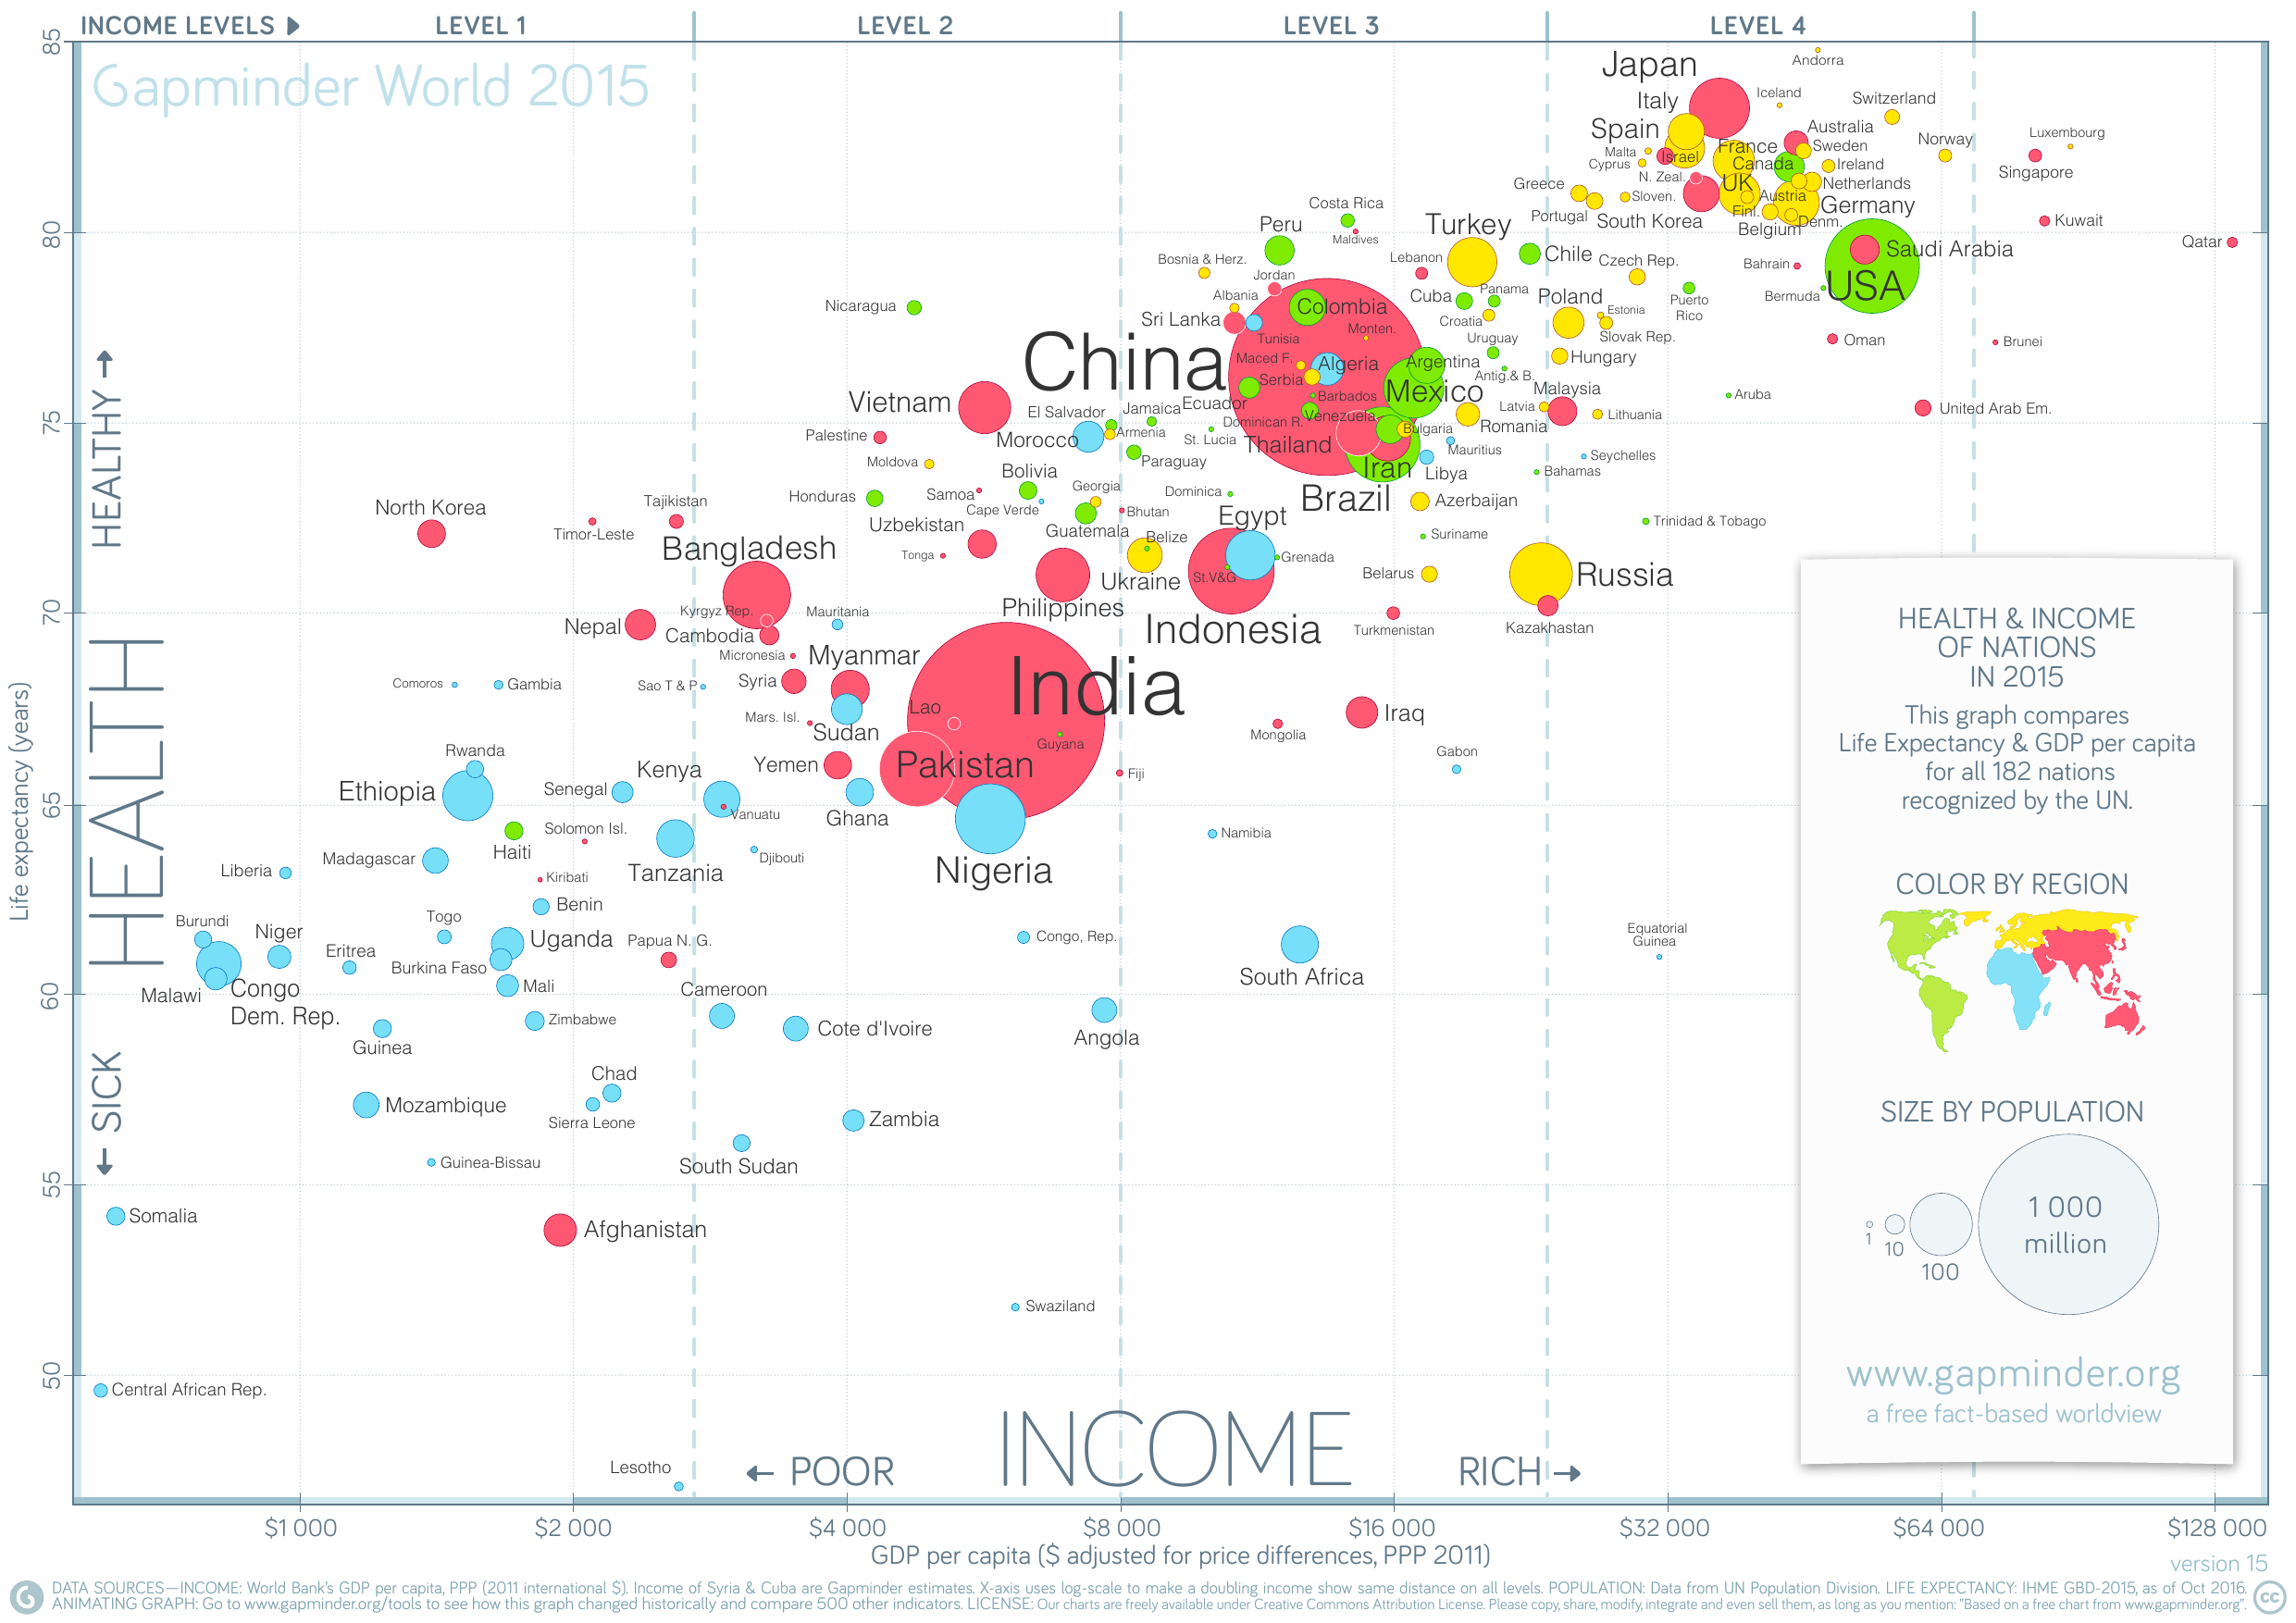
\includegraphics[width=1\linewidth]{images/countries-1} \end{center}

\begin{itemize}
\item
  O gráfico mostra como, em cada país, a saúde (mais precisamente, a expectativa de vida) se relaciona com a riqueza (mais precisamente, o PIB \emph{per capita}).
\item
  Além da expectativa de vida e o do PIB \emph{per capita}, o gráfico traz mais informações sobre cada país.
\item
  Cada país é representado por um ponto (a {\hl{geometria}}).
\item
  Informações sobre cada país são representadas por características do ponto correspondente (as {\hl{estéticas}}):

  \begin{longtable}[]{@{}lll@{}}
  \toprule
  Variável & Geometria & Estética \\
  \midrule
  \endhead
  PIB \emph{per capita} & ponto & posição x \\
  Expectativa de vida & ponto & posição y \\
  População & ponto & tamanho \\
  Continente & ponto & cor \\
  \bottomrule
  \end{longtable}
\item
  Você pode usar outras estéticas para representar informações:

  \begin{itemize}
  \tightlist
  \item
    Cor de preenchimento.
  \item
    Cor do traço.
  \item
    Tipo do traço (sólido, pontilhado, tracejado etc.).
  \item
    Forma (círculo, quadrado, triângulo etc.).
  \item
    Opacidade.
  \item
    etc.
  \end{itemize}
\item
  Você pode usar outras geometrias:

  \begin{itemize}
  \tightlist
  \item
    Linhas.
  \item
    Barras ou colunas.
  \item
    Caixas.
  \item
    etc.
  \end{itemize}
\end{itemize}

\hypertarget{escalas-scales}{%
\subsection{\texorpdfstring{Escalas (\emph{scales})}{Escalas (scales)}}\label{escalas-scales}}

\begin{itemize}
\item
  As escalas controlam os detalhes da aparência da geometria e do mapeamento (eixos, cores etc.).
\item
  Os eixos do gráfico acima são escalas {\hl{contínuas}}, com valores reais.
\item
  Observe o eixo horizontal. Os valores não aumentam linearmente, mas sim exponencialmente: cada passo à direita equivale a \emph{dobrar} o valor do PIB. O eixo horizontal segue uma {\hl{escala logarítmica}}.
\item
  Os tamanhos dos pontos formam uma escala {\hl{discreta}}, com $4$ valores possíveis (veja a legenda no canto inferior direito do gráfico).
\item
  As cores também formam uma escala discreta.
\end{itemize}

\hypertarget{ruxf3tulos-labels}{%
\subsection{\texorpdfstring{Rótulos (\emph{labels})}{Rótulos (labels)}}\label{ruxf3tulos-labels}}

\begin{itemize}
\item
  O gráfico também representa informação na forma de texto.
\item
  Além de rótulos (por exemplo, o texto que identifica cada eixo), {\hl{o texto também pode, ele mesmo, ser uma geometria, com suas próprias estéticas:}} observe como o nome de cada país é escrito em um tamanho proporcional à sua população.
\end{itemize}

\hypertarget{outros-componentes}{%
\subsection{Outros componentes}\label{outros-componentes}}

\begin{itemize}
\item
  Coordenadas:

  \begin{itemize}
  \item
    Este gráfico usa {\hl{coordenadas cartesianas}}, com eixos $x$ e $y$.
  \item
    Existem gráficos que usam um sistema de {\hl{coordenadas polares}}.
  \end{itemize}
\item
  Temas:

  \begin{itemize}
  \item
    Incluem todos os elementos ``decorativos'': cor de fundo, linhas de grade, etc. Ajudam a facilitar a leitura e a interpretação.
  \item
    No gráfico acima, um detalhe interessante do tema é a divisão de cada eixo em segmentos claros e segmentos escuros.
  \end{itemize}
\item
  Legendas (\emph{guides}).
\item
  Facetas:

  \begin{itemize}
  \item
    Às vezes, um gráfico é composto por múltiplos subgráficos.
  \item
    Cada subgráfico é uma {\hl{faceta}}.
  \item
    Facetas evitam que informações demais sejam apresentadas no mesmo lugar.
  \end{itemize}
\end{itemize}

\hypertarget{mamiferos}{%
\section{Conjunto de dados}\label{mamiferos}}

\begin{itemize}
\item
  Nossos exemplos de gráficos vão usar dados sobre o sono de diversos mamíferos.
\item
  O conjunto de dados se chama \texttt{msleep} e está incluído no pacote \texttt{ggplot2}.
\item
  Para ver a documentação, digite

\begin{Shaded}
\begin{Highlighting}[]
\FunctionTok{library}\NormalTok{(ggplot2)}
\NormalTok{?msleep}
\end{Highlighting}
\end{Shaded}
\item
  Vamos atribuir o conjunto de dados à variável \texttt{df}:

\begin{Shaded}
\begin{Highlighting}[]
\NormalTok{df }\OtherTok{\textless{}{-}}\NormalTok{ msleep}
\NormalTok{df}
\end{Highlighting}
\end{Shaded}

\begin{verbatim}
## # A tibble: 83 x 11
##   name             genus vore  order conservation sleep_total sleep_rem
##   <chr>            <chr> <chr> <chr> <chr>              <dbl>     <dbl>
## 1 Cheetah          Acin~ carni Carn~ lc                  12.1      NA  
## 2 Owl monkey       Aotus omni  Prim~ <NA>                17         1.8
## 3 Mountain beaver  Aplo~ herbi Rode~ nt                  14.4       2.4
## 4 Greater short-t~ Blar~ omni  Sori~ lc                  14.9       2.3
## 5 Cow              Bos   herbi Arti~ domesticated         4         0.7
## 6 Three-toed sloth Brad~ herbi Pilo~ <NA>                14.4       2.2
## # ... with 77 more rows, and 4 more variables: sleep_cycle <dbl>,
## #   awake <dbl>, brainwt <dbl>, bodywt <dbl>
\end{verbatim}
\item
  Vamos examinar a estrutura --- usando R base:

\begin{Shaded}
\begin{Highlighting}[]
\FunctionTok{str}\NormalTok{(df)}
\end{Highlighting}
\end{Shaded}

\begin{verbatim}
## tibble [83 x 11] (S3: tbl_df/tbl/data.frame)
##  $ name        : chr [1:83] "Cheetah" "Owl monkey" "Mountain beaver" ...
##  $ genus       : chr [1:83] "Acinonyx" "Aotus" "Aplodontia" ...
##  $ vore        : chr [1:83] "carni" "omni" "herbi" ...
##  $ order       : chr [1:83] "Carnivora" "Primates" "Rodentia" ...
##  $ conservation: chr [1:83] "lc" NA "nt" ...
##  $ sleep_total : num [1:83] 12,1 17 14,4 14,9 4 14,4 8,7 7 ...
##  $ sleep_rem   : num [1:83] NA 1,8 2,4 2,3 0,7 2,2 1,4 NA ...
##  $ sleep_cycle : num [1:83] NA NA NA 0,133 ...
##  $ awake       : num [1:83] 11,9 7 9,6 9,1 20 9,6 15,3 17 ...
##  $ brainwt     : num [1:83] NA 0,0155 NA 0,00029 0,423 NA NA NA ...
##  $ bodywt      : num [1:83] 50 0,48 1,35 0,019 ...
\end{verbatim}
\item
  Podemos usar \texttt{glimpse}, uma função do \texttt{tidyverse}:

\begin{Shaded}
\begin{Highlighting}[]
\FunctionTok{glimpse}\NormalTok{(df)}
\end{Highlighting}
\end{Shaded}

\begin{verbatim}
## Rows: 83
## Columns: 11
## $ name         <chr> "Cheetah", "Owl monkey", "Mountain beaver", "Gre~
## $ genus        <chr> "Acinonyx", "Aotus", "Aplodontia", "Blarina", "B~
## $ vore         <chr> "carni", "omni", "herbi", "omni", "herbi", "herb~
## $ order        <chr> "Carnivora", "Primates", "Rodentia", "Soricomorp~
## $ conservation <chr> "lc", NA, "nt", "lc", "domesticated", NA, "vu", ~
## $ sleep_total  <dbl> 12,1, 17,0, 14,4, 14,9, 4,0, 14,4, 8,7, 7,0, 10,~
## $ sleep_rem    <dbl> NA, 1,8, 2,4, 2,3, 0,7, 2,2, 1,4, NA, 2,9, NA, 0~
## $ sleep_cycle  <dbl> NA, NA, NA, 0,1333333, 0,6666667, 0,7666667, 0,3~
## $ awake        <dbl> 11,9, 7,0, 9,6, 9,1, 20,0, 9,6, 15,3, 17,0, 13,9~
## $ brainwt      <dbl> NA, 0,01550, NA, 0,00029, 0,42300, NA, NA, NA, 0~
## $ bodywt       <dbl> 50,000, 0,480, 1,350, 0,019, 600,000, 3,850, 20,~
\end{verbatim}
\item
  Para examinar só as primeiras linhas do \emph{data frame}:

\begin{Shaded}
\begin{Highlighting}[]
\FunctionTok{head}\NormalTok{(df)}
\end{Highlighting}
\end{Shaded}

\begin{verbatim}
## # A tibble: 6 x 11
##   name             genus vore  order conservation sleep_total sleep_rem
##   <chr>            <chr> <chr> <chr> <chr>              <dbl>     <dbl>
## 1 Cheetah          Acin~ carni Carn~ lc                  12.1      NA  
## 2 Owl monkey       Aotus omni  Prim~ <NA>                17         1.8
## 3 Mountain beaver  Aplo~ herbi Rode~ nt                  14.4       2.4
## 4 Greater short-t~ Blar~ omni  Sori~ lc                  14.9       2.3
## 5 Cow              Bos   herbi Arti~ domesticated         4         0.7
## 6 Three-toed sloth Brad~ herbi Pilo~ <NA>                14.4       2.2
## # ... with 4 more variables: sleep_cycle <dbl>, awake <dbl>,
## #   brainwt <dbl>, bodywt <dbl>
\end{verbatim}
\item
  Para examinar o \emph{data frame} interativamente:

\begin{Shaded}
\begin{Highlighting}[]
\FunctionTok{view}\NormalTok{(df)}
\end{Highlighting}
\end{Shaded}
\item
  Podemos produzir um sumário dos dados usando o pacote \emph{summarytools} (que já foi carregado neste documento):

\begin{Shaded}
\begin{Highlighting}[]
\NormalTok{df }\SpecialCharTok{\%\textgreater{}\%} \FunctionTok{dfSummary}\NormalTok{() }\SpecialCharTok{\%\textgreater{}\%} \FunctionTok{print}\NormalTok{()}
\end{Highlighting}
\end{Shaded}

  \begin{longtable}[]{@{}
    >{\raggedright\arraybackslash}p{(\columnwidth - 6\tabcolsep) * \real{0.1928}}
    >{\raggedright\arraybackslash}p{(\columnwidth - 6\tabcolsep) * \real{0.3976}}
    >{\raggedright\arraybackslash}p{(\columnwidth - 6\tabcolsep) * \real{0.2771}}
    >{\raggedright\arraybackslash}p{(\columnwidth - 6\tabcolsep) * \real{0.1325}}@{}}
  \toprule
  \begin{minipage}[b]{\linewidth}\raggedright
  Variável
  \end{minipage} & \begin{minipage}[b]{\linewidth}\raggedright
  Estatísticas / Valores
  \end{minipage} & \begin{minipage}[b]{\linewidth}\raggedright
  Freqs (\% de Válidos)
  \end{minipage} & \begin{minipage}[b]{\linewidth}\raggedright
  Faltante
  \end{minipage} \\
  \midrule
  \endhead
  \begin{minipage}[t]{\linewidth}\raggedright
  name\\
  {[}character{]}\strut
  \end{minipage} & \begin{minipage}[t]{\linewidth}\raggedright
  1. African elephant\\
  2. African giant pouched rat\\
  3. African striped mouse\\
  4. Arctic fox\\
  5. Arctic ground squirrel\\
  6. Asian elephant\\
  7. Baboon\\
  8. Big brown bat\\
  9. Bottle-nosed dolphin\\
  10. Brazilian tapir\\
  {[} 73 outros {]}\strut
  \end{minipage} & \begin{minipage}[t]{\linewidth}\raggedright
  1 ( 1,2\%)\\
  1 ( 1,2\%)\\
  1 ( 1,2\%)\\
  1 ( 1,2\%)\\
  1 ( 1,2\%)\\
  1 ( 1,2\%)\\
  1 ( 1,2\%)\\
  1 ( 1,2\%)\\
  1 ( 1,2\%)\\
  1 ( 1,2\%)\\
  73 (88,0\%)\strut
  \end{minipage} & \begin{minipage}[t]{\linewidth}\raggedright
  0\\
  (0,0\%)\strut
  \end{minipage} \\
  \begin{minipage}[t]{\linewidth}\raggedright
  genus\\
  {[}character{]}\strut
  \end{minipage} & \begin{minipage}[t]{\linewidth}\raggedright
  1. Panthera\\
  2. Spermophilus\\
  3. Equus\\
  4. Vulpes\\
  5. Acinonyx\\
  6. Aotus\\
  7. Aplodontia\\
  8. Blarina\\
  9. Bos\\
  10. Bradypus\\
  {[} 67 outros {]}\strut
  \end{minipage} & \begin{minipage}[t]{\linewidth}\raggedright
  3 ( 3,6\%)\\
  3 ( 3,6\%)\\
  2 ( 2,4\%)\\
  2 ( 2,4\%)\\
  1 ( 1,2\%)\\
  1 ( 1,2\%)\\
  1 ( 1,2\%)\\
  1 ( 1,2\%)\\
  1 ( 1,2\%)\\
  1 ( 1,2\%)\\
  67 (80,7\%)\strut
  \end{minipage} & \begin{minipage}[t]{\linewidth}\raggedright
  0\\
  (0,0\%)\strut
  \end{minipage} \\
  \begin{minipage}[t]{\linewidth}\raggedright
  vore\\
  {[}character{]}\strut
  \end{minipage} & \begin{minipage}[t]{\linewidth}\raggedright
  1. carni\\
  2. herbi\\
  3. insecti\\
  4. omni\strut
  \end{minipage} & \begin{minipage}[t]{\linewidth}\raggedright
  19 (25,0\%)\\
  32 (42,1\%)\\
  5 ( 6,6\%)\\
  20 (26,3\%)\strut
  \end{minipage} & \begin{minipage}[t]{\linewidth}\raggedright
  7\\
  (8,4\%)\strut
  \end{minipage} \\
  \begin{minipage}[t]{\linewidth}\raggedright
  order\\
  {[}character{]}\strut
  \end{minipage} & \begin{minipage}[t]{\linewidth}\raggedright
  1. Rodentia\\
  2. Carnivora\\
  3. Primates\\
  4. Artiodactyla\\
  5. Soricomorpha\\
  6. Cetacea\\
  7. Hyracoidea\\
  8. Perissodactyla\\
  9. Chiroptera\\
  10. Cingulata\\
  {[} 9 outros {]}\strut
  \end{minipage} & \begin{minipage}[t]{\linewidth}\raggedright
  22 (26,5\%)\\
  12 (14,5\%)\\
  12 (14,5\%)\\
  6 ( 7,2\%)\\
  5 ( 6,0\%)\\
  3 ( 3,6\%)\\
  3 ( 3,6\%)\\
  3 ( 3,6\%)\\
  2 ( 2,4\%)\\
  2 ( 2,4\%)\\
  13 (15,7\%)\strut
  \end{minipage} & \begin{minipage}[t]{\linewidth}\raggedright
  0\\
  (0,0\%)\strut
  \end{minipage} \\
  \begin{minipage}[t]{\linewidth}\raggedright
  conservation\\
  {[}character{]}\strut
  \end{minipage} & \begin{minipage}[t]{\linewidth}\raggedright
  1. cd\\
  2. domesticated\\
  3. en\\
  4. lc\\
  5. nt\\
  6. vu\strut
  \end{minipage} & \begin{minipage}[t]{\linewidth}\raggedright
  2 ( 3,7\%)\\
  10 (18,5\%)\\
  4 ( 7,4\%)\\
  27 (50,0\%)\\
  4 ( 7,4\%)\\
  7 (13,0\%)\strut
  \end{minipage} & \begin{minipage}[t]{\linewidth}\raggedright
  29\\
  (34,9\%)\strut
  \end{minipage} \\
  \begin{minipage}[t]{\linewidth}\raggedright
  sleep\_total\\
  {[}numeric{]}\strut
  \end{minipage} & \begin{minipage}[t]{\linewidth}\raggedright
  Média (dp) : 10,4 (4,5)\\
  mín \textless{} mediana \textless{} máx:\\
  1,9 \textless{} 10,1 \textless{} 19,9\\
  IQE (CV) : 5,9 (0,4)\strut
  \end{minipage} & 65 valores distintos & \begin{minipage}[t]{\linewidth}\raggedright
  0\\
  (0,0\%)\strut
  \end{minipage} \\
  \begin{minipage}[t]{\linewidth}\raggedright
  sleep\_rem\\
  {[}numeric{]}\strut
  \end{minipage} & \begin{minipage}[t]{\linewidth}\raggedright
  Média (dp) : 1,9 (1,3)\\
  mín \textless{} mediana \textless{} máx:\\
  0,1 \textless{} 1,5 \textless{} 6,6\\
  IQE (CV) : 1,5 (0,7)\strut
  \end{minipage} & 32 valores distintos & \begin{minipage}[t]{\linewidth}\raggedright
  22\\
  (26,5\%)\strut
  \end{minipage} \\
  \begin{minipage}[t]{\linewidth}\raggedright
  sleep\_cycle\\
  {[}numeric{]}\strut
  \end{minipage} & \begin{minipage}[t]{\linewidth}\raggedright
  Média (dp) : 0,4 (0,4)\\
  mín \textless{} mediana \textless{} máx:\\
  0,1 \textless{} 0,3 \textless{} 1,5\\
  IQE (CV) : 0,4 (0,8)\strut
  \end{minipage} & 22 valores distintos & \begin{minipage}[t]{\linewidth}\raggedright
  51\\
  (61,4\%)\strut
  \end{minipage} \\
  \begin{minipage}[t]{\linewidth}\raggedright
  awake\\
  {[}numeric{]}\strut
  \end{minipage} & \begin{minipage}[t]{\linewidth}\raggedright
  Média (dp) : 13,6 (4,5)\\
  mín \textless{} mediana \textless{} máx:\\
  4,1 \textless{} 13,9 \textless{} 22,1\\
  IQE (CV) : 5,9 (0,3)\strut
  \end{minipage} & 65 valores distintos & \begin{minipage}[t]{\linewidth}\raggedright
  0\\
  (0,0\%)\strut
  \end{minipage} \\
  \begin{minipage}[t]{\linewidth}\raggedright
  brainwt\\
  {[}numeric{]}\strut
  \end{minipage} & \begin{minipage}[t]{\linewidth}\raggedright
  Média (dp) : 0,3 (1)\\
  mín \textless{} mediana \textless{} máx:\\
  0 \textless{} 0 \textless{} 5,7\\
  IQE (CV) : 0,1 (3,5)\strut
  \end{minipage} & 53 valores distintos & \begin{minipage}[t]{\linewidth}\raggedright
  27\\
  (32,5\%)\strut
  \end{minipage} \\
  \begin{minipage}[t]{\linewidth}\raggedright
  bodywt\\
  {[}numeric{]}\strut
  \end{minipage} & \begin{minipage}[t]{\linewidth}\raggedright
  Média (dp) : 166,1 (786,8)\\
  mín \textless{} mediana \textless{} máx:\\
  0 \textless{} 1,7 \textless{} 6654\\
  IQE (CV) : 41,6 (4,7)\strut
  \end{minipage} & 82 valores distintos & \begin{minipage}[t]{\linewidth}\raggedright
  0\\
  (0,0\%)\strut
  \end{minipage} \\
  \bottomrule
  \end{longtable}
\item
  Vemos que há muitos \texttt{NA} em diversas variáveis. Para nossos exemplos simples de visualização, vamos usar as colunas

  \begin{itemize}
  \tightlist
  \item
    \texttt{name}
  \item
    \texttt{genus}
  \item
    \texttt{order}
  \item
    \texttt{sleep\_total}
  \item
    \texttt{awake}
  \item
    \texttt{bodywt}
  \item
    \texttt{brainwt}
  \end{itemize}
\item
  Mas\ldots{} a coluna que mostra a dieta (\texttt{vore}) tem só 7 \texttt{NA}. Quais são?

\begin{Shaded}
\begin{Highlighting}[]
\NormalTok{df }\SpecialCharTok{\%\textgreater{}\%} 
  \FunctionTok{filter}\NormalTok{(}\FunctionTok{is.na}\NormalTok{(vore)) }\SpecialCharTok{\%\textgreater{}\%} 
  \FunctionTok{select}\NormalTok{(name)}
\end{Highlighting}
\end{Shaded}

\begin{verbatim}
## # A tibble: 7 x 1
##   name           
##   <chr>          
## 1 Vesper mouse   
## 2 Desert hedgehog
## 3 Deer mouse     
## 4 Phalanger      
## 5 Rock hyrax     
## 6 Mole rat       
## # ... with 1 more row
\end{verbatim}
\item
  OK. Vamos manter a coluna \texttt{vore} também, apesar dos \texttt{NA}. Quando formos usar esta variável, tomaremos cuidado.
\item
  Também\ldots{} a coluna \texttt{bodywt} tem 0 como valor mínimo. Como assim?

\begin{Shaded}
\begin{Highlighting}[]
\NormalTok{df }\SpecialCharTok{\%\textgreater{}\%} 
  \FunctionTok{filter}\NormalTok{(bodywt }\SpecialCharTok{\textless{}} \DecValTok{1}\NormalTok{) }\SpecialCharTok{\%\textgreater{}\%} 
  \FunctionTok{select}\NormalTok{(name, bodywt) }\SpecialCharTok{\%\textgreater{}\%} 
  \FunctionTok{arrange}\NormalTok{(bodywt)}
\end{Highlighting}
\end{Shaded}

\begin{verbatim}
## # A tibble: 35 x 2
##   name                       bodywt
##   <chr>                       <dbl>
## 1 Lesser short-tailed shrew   0.005
## 2 Little brown bat            0.01 
## 3 Greater short-tailed shrew  0.019
## 4 Deer mouse                  0.021
## 5 House mouse                 0.022
## 6 Big brown bat               0.023
## # ... with 29 more rows
\end{verbatim}
\item
  Ah, sem problema. A função \texttt{dfSummary} arredondou estes pesos para 0. Os valores de verdade ainda estão na \emph{tibble}.
\item
  Vamos criar uma \emph{tibble} nova, só com as colunas que nos interessam:

\begin{Shaded}
\begin{Highlighting}[]
\NormalTok{sono }\OtherTok{\textless{}{-}}\NormalTok{ df }\SpecialCharTok{\%\textgreater{}\%} 
  \FunctionTok{select}\NormalTok{(}
\NormalTok{    name, order, genus, vore, bodywt, }
\NormalTok{    brainwt, awake, sleep\_total}
\NormalTok{  )}
\end{Highlighting}
\end{Shaded}
\item
  Vamos ver o sumário:

\begin{Shaded}
\begin{Highlighting}[]
\NormalTok{sono }\SpecialCharTok{\%\textgreater{}\%} \FunctionTok{dfSummary}\NormalTok{() }\SpecialCharTok{\%\textgreater{}\%} \FunctionTok{print}\NormalTok{()}
\end{Highlighting}
\end{Shaded}

  \begin{longtable}[]{@{}
    >{\raggedright\arraybackslash}p{(\columnwidth - 6\tabcolsep) * \real{0.1829}}
    >{\raggedright\arraybackslash}p{(\columnwidth - 6\tabcolsep) * \real{0.4024}}
    >{\raggedright\arraybackslash}p{(\columnwidth - 6\tabcolsep) * \real{0.2805}}
    >{\raggedright\arraybackslash}p{(\columnwidth - 6\tabcolsep) * \real{0.1341}}@{}}
  \toprule
  \begin{minipage}[b]{\linewidth}\raggedright
  Variável
  \end{minipage} & \begin{minipage}[b]{\linewidth}\raggedright
  Estatísticas / Valores
  \end{minipage} & \begin{minipage}[b]{\linewidth}\raggedright
  Freqs (\% de Válidos)
  \end{minipage} & \begin{minipage}[b]{\linewidth}\raggedright
  Faltante
  \end{minipage} \\
  \midrule
  \endhead
  \begin{minipage}[t]{\linewidth}\raggedright
  name\\
  {[}character{]}\strut
  \end{minipage} & \begin{minipage}[t]{\linewidth}\raggedright
  1. African elephant\\
  2. African giant pouched rat\\
  3. African striped mouse\\
  4. Arctic fox\\
  5. Arctic ground squirrel\\
  6. Asian elephant\\
  7. Baboon\\
  8. Big brown bat\\
  9. Bottle-nosed dolphin\\
  10. Brazilian tapir\\
  {[} 73 outros {]}\strut
  \end{minipage} & \begin{minipage}[t]{\linewidth}\raggedright
  1 ( 1,2\%)\\
  1 ( 1,2\%)\\
  1 ( 1,2\%)\\
  1 ( 1,2\%)\\
  1 ( 1,2\%)\\
  1 ( 1,2\%)\\
  1 ( 1,2\%)\\
  1 ( 1,2\%)\\
  1 ( 1,2\%)\\
  1 ( 1,2\%)\\
  73 (88,0\%)\strut
  \end{minipage} & \begin{minipage}[t]{\linewidth}\raggedright
  0\\
  (0,0\%)\strut
  \end{minipage} \\
  \begin{minipage}[t]{\linewidth}\raggedright
  order\\
  {[}character{]}\strut
  \end{minipage} & \begin{minipage}[t]{\linewidth}\raggedright
  1. Rodentia\\
  2. Carnivora\\
  3. Primates\\
  4. Artiodactyla\\
  5. Soricomorpha\\
  6. Cetacea\\
  7. Hyracoidea\\
  8. Perissodactyla\\
  9. Chiroptera\\
  10. Cingulata\\
  {[} 9 outros {]}\strut
  \end{minipage} & \begin{minipage}[t]{\linewidth}\raggedright
  22 (26,5\%)\\
  12 (14,5\%)\\
  12 (14,5\%)\\
  6 ( 7,2\%)\\
  5 ( 6,0\%)\\
  3 ( 3,6\%)\\
  3 ( 3,6\%)\\
  3 ( 3,6\%)\\
  2 ( 2,4\%)\\
  2 ( 2,4\%)\\
  13 (15,7\%)\strut
  \end{minipage} & \begin{minipage}[t]{\linewidth}\raggedright
  0\\
  (0,0\%)\strut
  \end{minipage} \\
  \begin{minipage}[t]{\linewidth}\raggedright
  genus\\
  {[}character{]}\strut
  \end{minipage} & \begin{minipage}[t]{\linewidth}\raggedright
  1. Panthera\\
  2. Spermophilus\\
  3. Equus\\
  4. Vulpes\\
  5. Acinonyx\\
  6. Aotus\\
  7. Aplodontia\\
  8. Blarina\\
  9. Bos\\
  10. Bradypus\\
  {[} 67 outros {]}\strut
  \end{minipage} & \begin{minipage}[t]{\linewidth}\raggedright
  3 ( 3,6\%)\\
  3 ( 3,6\%)\\
  2 ( 2,4\%)\\
  2 ( 2,4\%)\\
  1 ( 1,2\%)\\
  1 ( 1,2\%)\\
  1 ( 1,2\%)\\
  1 ( 1,2\%)\\
  1 ( 1,2\%)\\
  1 ( 1,2\%)\\
  67 (80,7\%)\strut
  \end{minipage} & \begin{minipage}[t]{\linewidth}\raggedright
  0\\
  (0,0\%)\strut
  \end{minipage} \\
  \begin{minipage}[t]{\linewidth}\raggedright
  vore\\
  {[}character{]}\strut
  \end{minipage} & \begin{minipage}[t]{\linewidth}\raggedright
  1. carni\\
  2. herbi\\
  3. insecti\\
  4. omni\strut
  \end{minipage} & \begin{minipage}[t]{\linewidth}\raggedright
  19 (25,0\%)\\
  32 (42,1\%)\\
  5 ( 6,6\%)\\
  20 (26,3\%)\strut
  \end{minipage} & \begin{minipage}[t]{\linewidth}\raggedright
  7\\
  (8,4\%)\strut
  \end{minipage} \\
  \begin{minipage}[t]{\linewidth}\raggedright
  bodywt\\
  {[}numeric{]}\strut
  \end{minipage} & \begin{minipage}[t]{\linewidth}\raggedright
  Média (dp) : 166,1 (786,8)\\
  mín \textless{} mediana \textless{} máx:\\
  0 \textless{} 1,7 \textless{} 6654\\
  IQE (CV) : 41,6 (4,7)\strut
  \end{minipage} & 82 valores distintos & \begin{minipage}[t]{\linewidth}\raggedright
  0\\
  (0,0\%)\strut
  \end{minipage} \\
  \begin{minipage}[t]{\linewidth}\raggedright
  brainwt\\
  {[}numeric{]}\strut
  \end{minipage} & \begin{minipage}[t]{\linewidth}\raggedright
  Média (dp) : 0,3 (1)\\
  mín \textless{} mediana \textless{} máx:\\
  0 \textless{} 0 \textless{} 5,7\\
  IQE (CV) : 0,1 (3,5)\strut
  \end{minipage} & 53 valores distintos & \begin{minipage}[t]{\linewidth}\raggedright
  27\\
  (32,5\%)\strut
  \end{minipage} \\
  \begin{minipage}[t]{\linewidth}\raggedright
  awake\\
  {[}numeric{]}\strut
  \end{minipage} & \begin{minipage}[t]{\linewidth}\raggedright
  Média (dp) : 13,6 (4,5)\\
  mín \textless{} mediana \textless{} máx:\\
  4,1 \textless{} 13,9 \textless{} 22,1\\
  IQE (CV) : 5,9 (0,3)\strut
  \end{minipage} & 65 valores distintos & \begin{minipage}[t]{\linewidth}\raggedright
  0\\
  (0,0\%)\strut
  \end{minipage} \\
  \begin{minipage}[t]{\linewidth}\raggedright
  sleep\_total\\
  {[}numeric{]}\strut
  \end{minipage} & \begin{minipage}[t]{\linewidth}\raggedright
  Média (dp) : 10,4 (4,5)\\
  mín \textless{} mediana \textless{} máx:\\
  1,9 \textless{} 10,1 \textless{} 19,9\\
  IQE (CV) : 5,9 (0,4)\strut
  \end{minipage} & 65 valores distintos & \begin{minipage}[t]{\linewidth}\raggedright
  0\\
  (0,0\%)\strut
  \end{minipage} \\
  \bottomrule
  \end{longtable}
\end{itemize}

\hypertarget{gruxe1ficos-de-dispersuxe3o-scatter-plots}{%
\section{\texorpdfstring{Gráficos de dispersão (\emph{scatter plots})}{Gráficos de dispersão (scatter plots)}}\label{gruxe1ficos-de-dispersuxe3o-scatter-plots}}

\begin{itemize}
\item
  Servem para visualizar a \emph{relação} entre {\hl{duas variáveis quantitativas.}}
\item
  {\hl{Essa relação \emph{não} é necessariamente de causa e efeito.}}
\item
  Isto é, a variável do eixo horizontal não determina, necessariamente, os valores da variável do eixo vertical.
\item
  Pense em {\hl{associação}}, {\hl{correlação}}, não em causalidade.
\item
  Troque as variáveis de eixo, se ajudar a deixar isto claro.
\end{itemize}

\hypertarget{horas-de-sono-e-peso-corporal}{%
\subsection{Horas de sono e peso corporal}\label{horas-de-sono-e-peso-corporal}}

\begin{itemize}
\item
  Como as variáveis \texttt{sleep\_total} e \texttt{bodywt} estão relacionadas?

\begin{Shaded}
\begin{Highlighting}[]
\NormalTok{sono }\SpecialCharTok{\%\textgreater{}\%} 
  \FunctionTok{ggplot}\NormalTok{(}\FunctionTok{aes}\NormalTok{(}\AttributeTok{x =}\NormalTok{ bodywt, }\AttributeTok{y =}\NormalTok{ sleep\_total))}
\end{Highlighting}
\end{Shaded}

  \begin{center}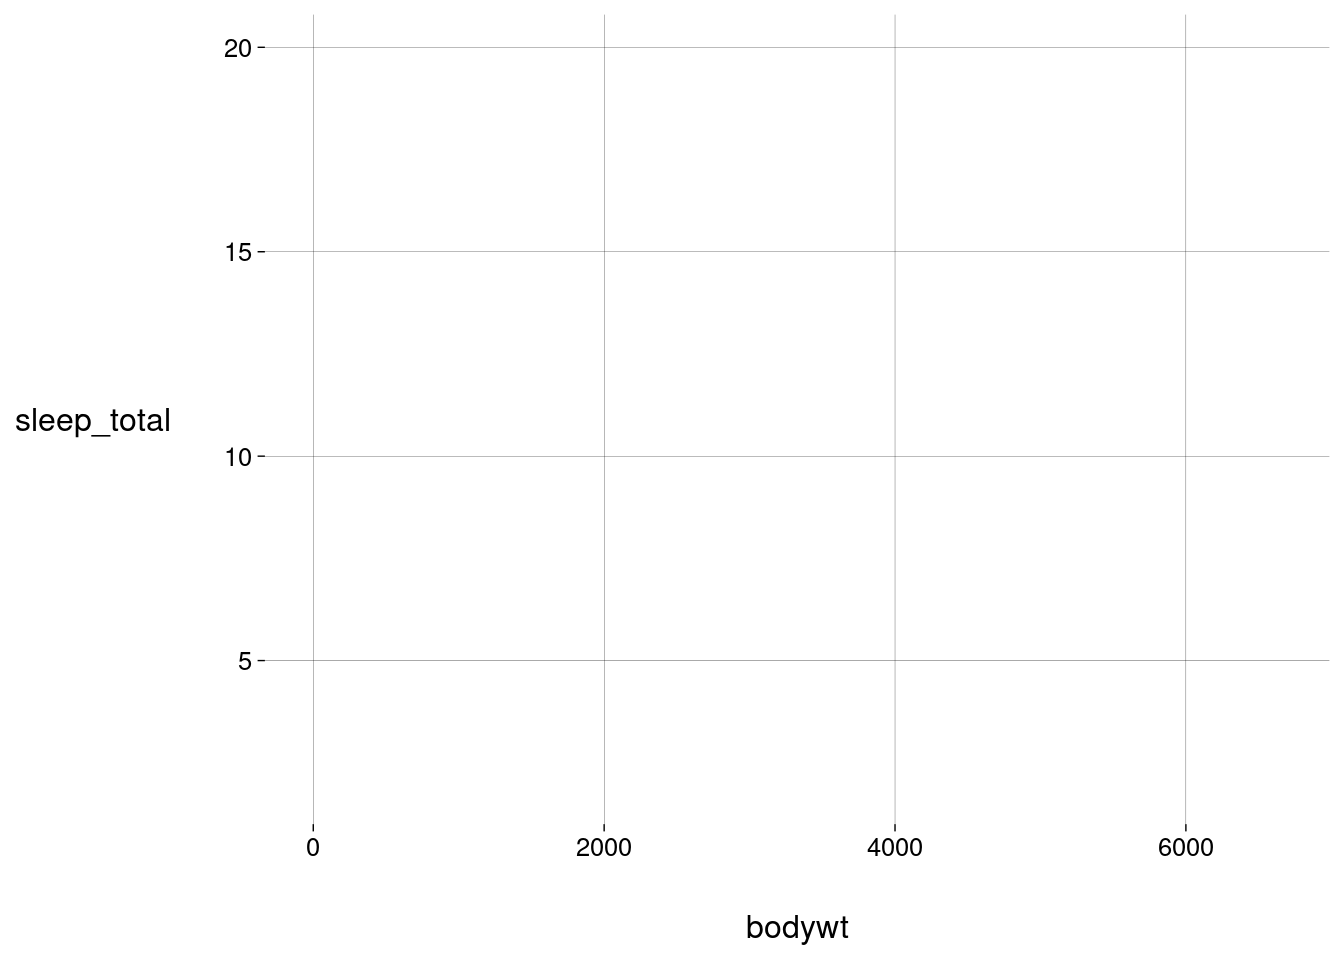
\includegraphics[width=1\linewidth]{_main_files/figure-latex/sono-peso-plot-1-1} \end{center}
\item
  O que houve? Cadê os pontos?
\item
  O problema foi que só especificamos o mapeamento estético (com \texttt{aes}, que são as iniciais de \emph{aesthetics}). {\hl{Faltou a geometria.}}

\begin{Shaded}
\begin{Highlighting}[]
\NormalTok{sono }\SpecialCharTok{\%\textgreater{}\%} 
  \FunctionTok{ggplot}\NormalTok{(}\FunctionTok{aes}\NormalTok{(}\AttributeTok{x =}\NormalTok{ bodywt, }\AttributeTok{y =}\NormalTok{ sleep\_total)) }\SpecialCharTok{+}
  \FunctionTok{geom\_point}\NormalTok{()}
\end{Highlighting}
\end{Shaded}

  \begin{center}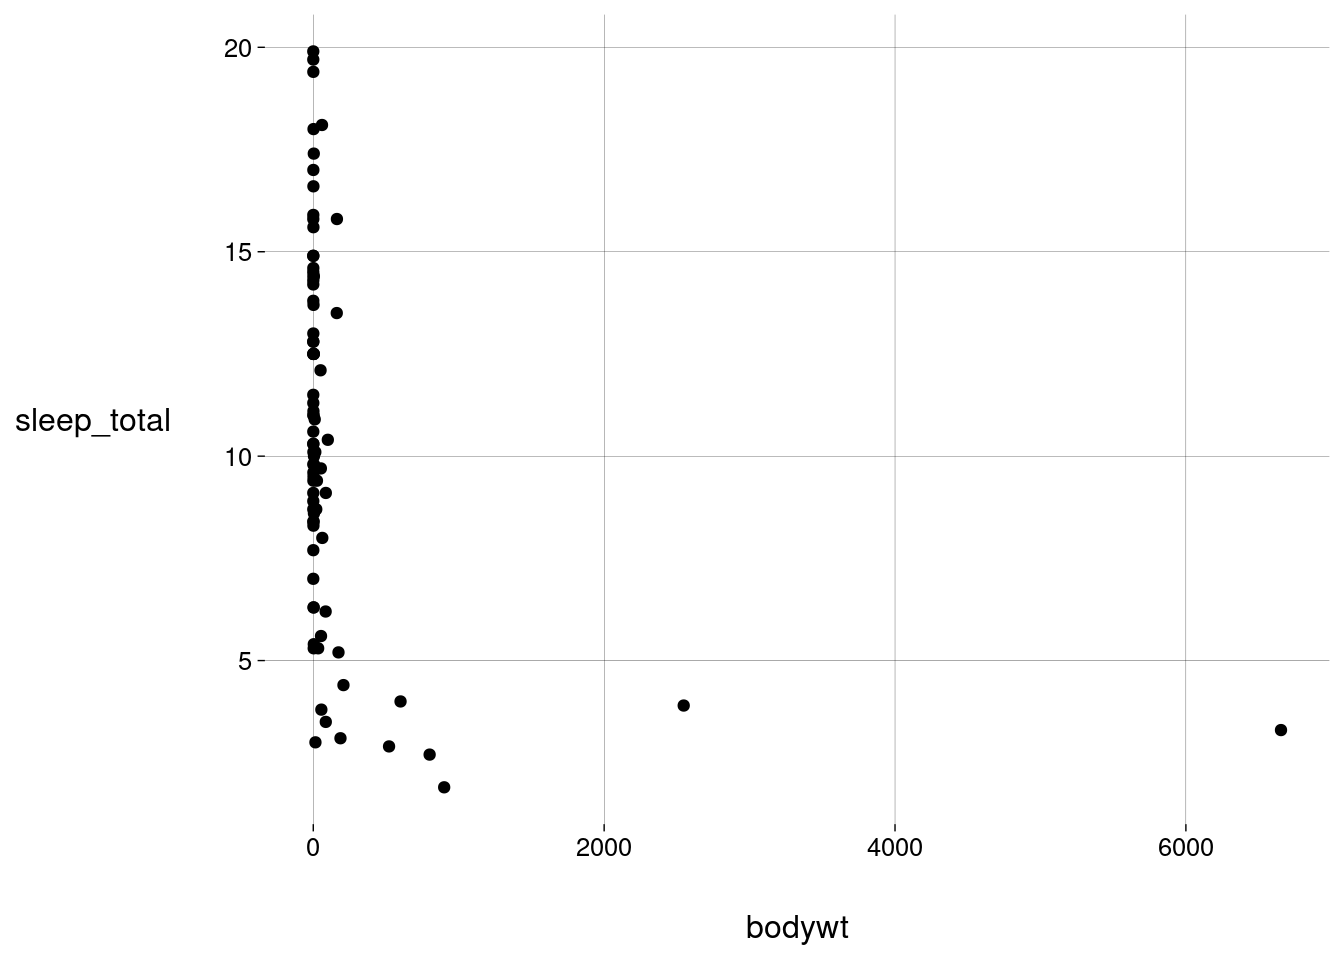
\includegraphics[width=1\linewidth]{_main_files/figure-latex/sono-peso-plot-2-1} \end{center}
\item
  Que horror.
\item
  A única coisa que percebemos aqui é que os mamíferos muito pesados dormem menos de $5$ horas por noite.
\item
  Estes animais muito pesados estão estragando a escala do eixo $x$.
\item
  Que animais são estes?

\begin{Shaded}
\begin{Highlighting}[]
\NormalTok{sono }\SpecialCharTok{\%\textgreater{}\%} 
  \FunctionTok{filter}\NormalTok{(bodywt }\SpecialCharTok{\textgreater{}} \DecValTok{250}\NormalTok{) }\SpecialCharTok{\%\textgreater{}\%} 
  \FunctionTok{select}\NormalTok{(name, bodywt) }\SpecialCharTok{\%\textgreater{}\%} 
  \FunctionTok{arrange}\NormalTok{(bodywt)}
\end{Highlighting}
\end{Shaded}

\begin{verbatim}
## # A tibble: 6 x 2
##   name             bodywt
##   <chr>             <dbl>
## 1 Horse              521 
## 2 Cow                600 
## 3 Pilot whale        800 
## 4 Giraffe            900.
## 5 Asian elephant    2547 
## 6 African elephant  6654
\end{verbatim}
\item
  Além disso, há muitos pontos sobrepostos. Em bom português, temos um problema de \emph{overplotting}.
\item
  Existem diversas maneiras de lidar com isso.
\item
  A primeira delas é {\hl{alterando a opacidade dos pontos}}. Isto é um ajuste na geometria apenas, pois a opacidade, aqui, não representa informação nenhuma.

\begin{Shaded}
\begin{Highlighting}[]
\NormalTok{sono }\SpecialCharTok{\%\textgreater{}\%} 
  \FunctionTok{ggplot}\NormalTok{(}\FunctionTok{aes}\NormalTok{(}\AttributeTok{x =}\NormalTok{ bodywt, }\AttributeTok{y =}\NormalTok{ sleep\_total)) }\SpecialCharTok{+}
    \FunctionTok{geom\_point}\NormalTok{(}\AttributeTok{alpha =} \FloatTok{0.2}\NormalTok{)}
\end{Highlighting}
\end{Shaded}

  \begin{center}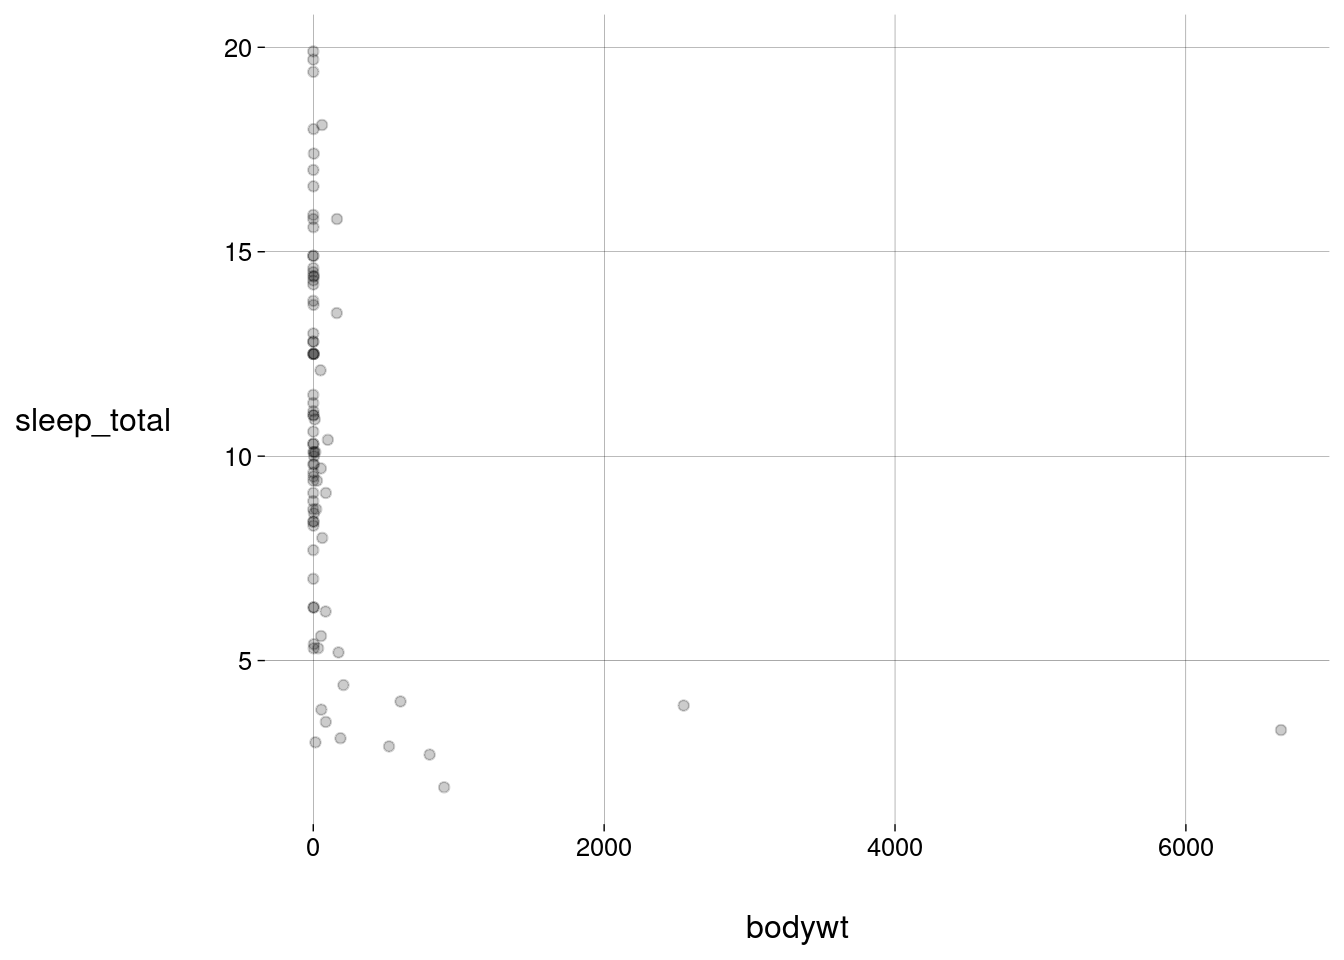
\includegraphics[width=1\linewidth]{_main_files/figure-latex/sono-peso-plot-alfa-1} \end{center}
\item
  Outra maneira é usar \texttt{geom\_jitter} em vez de \texttt{geom\_point}. ``\emph{Jitter}'' significa ``tremer''. As posições dos pontos são ligeiramente perturbadas, para evitar colisões. Perdemos precisão, mas a visualização fica melhor.

\begin{Shaded}
\begin{Highlighting}[]
\NormalTok{sono }\SpecialCharTok{\%\textgreater{}\%} 
  \FunctionTok{ggplot}\NormalTok{(}\FunctionTok{aes}\NormalTok{(}\AttributeTok{x =}\NormalTok{ bodywt, }\AttributeTok{y =}\NormalTok{ sleep\_total)) }\SpecialCharTok{+}
    \FunctionTok{geom\_jitter}\NormalTok{(}\AttributeTok{width =} \DecValTok{100}\NormalTok{)}
\end{Highlighting}
\end{Shaded}

  \begin{center}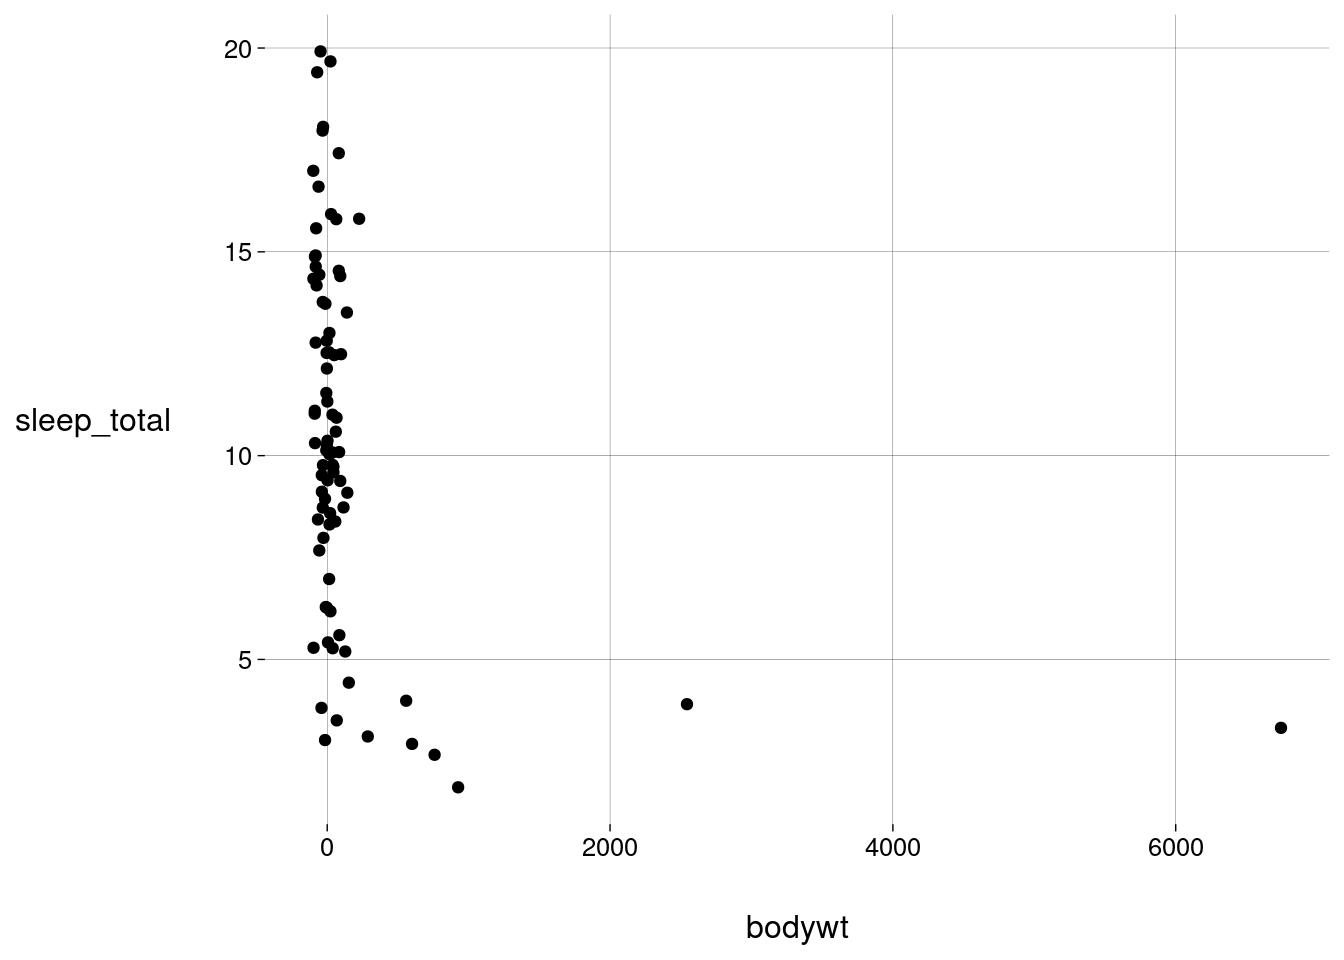
\includegraphics[width=1\linewidth]{_main_files/figure-latex/sono-peso-plot-jitter-1} \end{center}
\item
  Vamos mudar os limites do gráfico para nos concentrarmos nos animais menos pesados. Observe que {\hl{isto é um ajuste na escala}}.

\begin{Shaded}
\begin{Highlighting}[]
\NormalTok{sono }\SpecialCharTok{\%\textgreater{}\%} 
  \FunctionTok{ggplot}\NormalTok{(}\FunctionTok{aes}\NormalTok{(}\AttributeTok{x =}\NormalTok{ bodywt, }\AttributeTok{y =}\NormalTok{ sleep\_total)) }\SpecialCharTok{+}
    \FunctionTok{geom\_point}\NormalTok{() }\SpecialCharTok{+}
    \FunctionTok{scale\_x\_continuous}\NormalTok{(}\AttributeTok{limits =} \FunctionTok{c}\NormalTok{(}\DecValTok{0}\NormalTok{, }\DecValTok{200}\NormalTok{))}
\end{Highlighting}
\end{Shaded}

\begin{verbatim}
## Warning: Removed 7 rows containing missing values (geom_point).
\end{verbatim}

  \begin{center}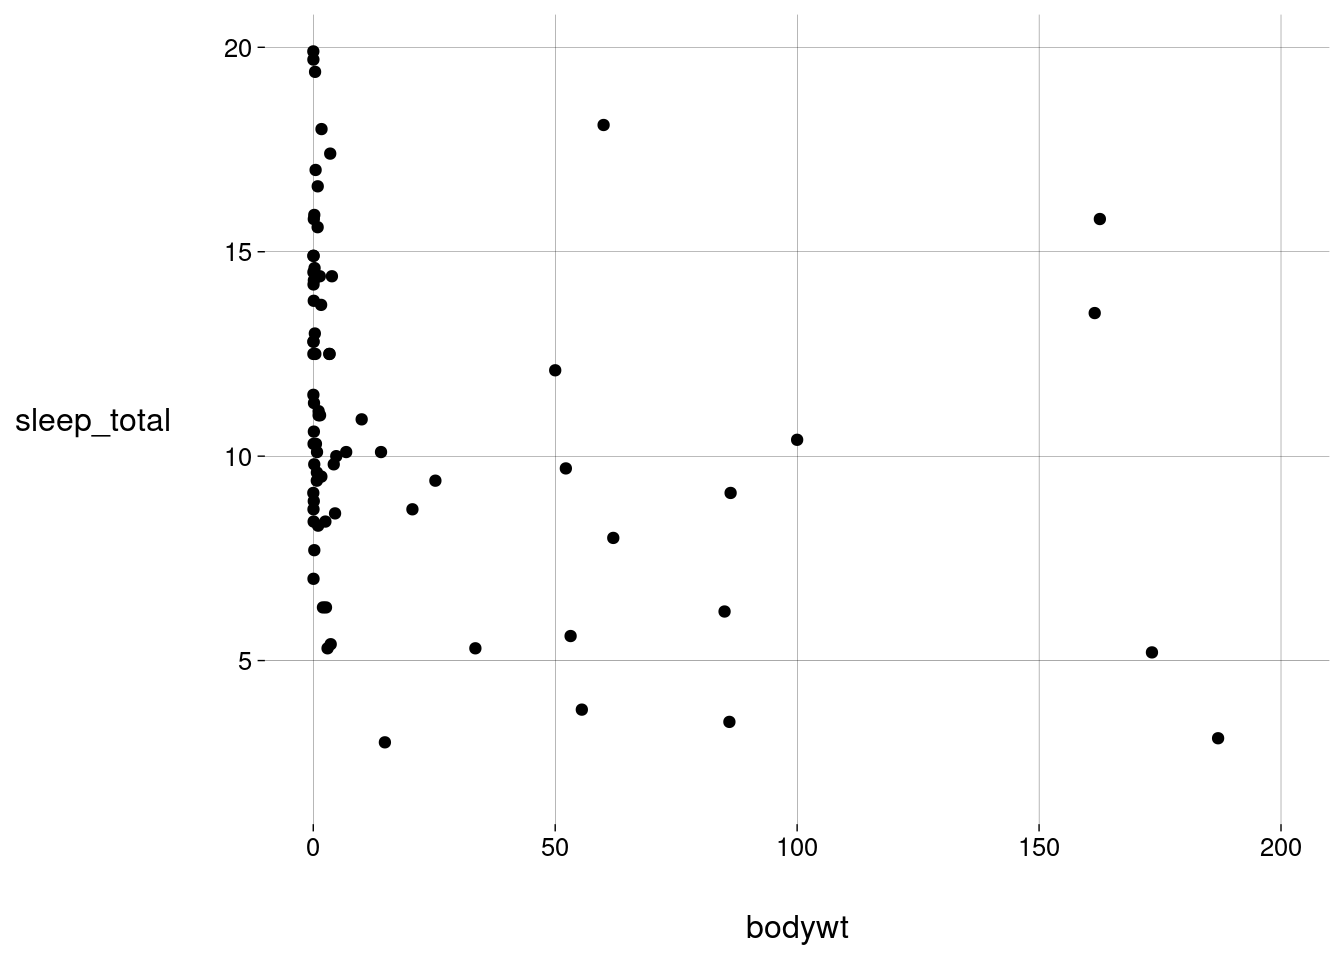
\includegraphics[width=1\linewidth]{_main_files/figure-latex/sono-peso-plot-3-1} \end{center}
\item
  Nestes limites, a relação entre horas de sono e peso não é mais tão pronunciada.
\end{itemize}

\hypertarget{horas-de-sono-e-peso-corporal-para-animais-pequenos}{%
\subsection{Horas de sono e peso corporal para animais pequenos}\label{horas-de-sono-e-peso-corporal-para-animais-pequenos}}

\begin{itemize}
\item
  Vamos restringir o gráfico a animais com no máximo $5$kg.

\begin{Shaded}
\begin{Highlighting}[]
\NormalTok{limite }\OtherTok{\textless{}{-}} \DecValTok{5}
\end{Highlighting}
\end{Shaded}
\item
  Em vez de mudar a escala do gráfico, vamos filtrar as linhas do \emph{data frame}:

\begin{Shaded}
\begin{Highlighting}[]
\NormalTok{sono }\SpecialCharTok{\%\textgreater{}\%} 
  \FunctionTok{filter}\NormalTok{(bodywt }\SpecialCharTok{\textless{}}\NormalTok{ limite) }\SpecialCharTok{\%\textgreater{}\%} 
  \FunctionTok{ggplot}\NormalTok{(}\FunctionTok{aes}\NormalTok{(}\AttributeTok{x =}\NormalTok{ bodywt, }\AttributeTok{y =}\NormalTok{ sleep\_total)) }\SpecialCharTok{+}
    \FunctionTok{geom\_point}\NormalTok{()}
\end{Highlighting}
\end{Shaded}

  \begin{center}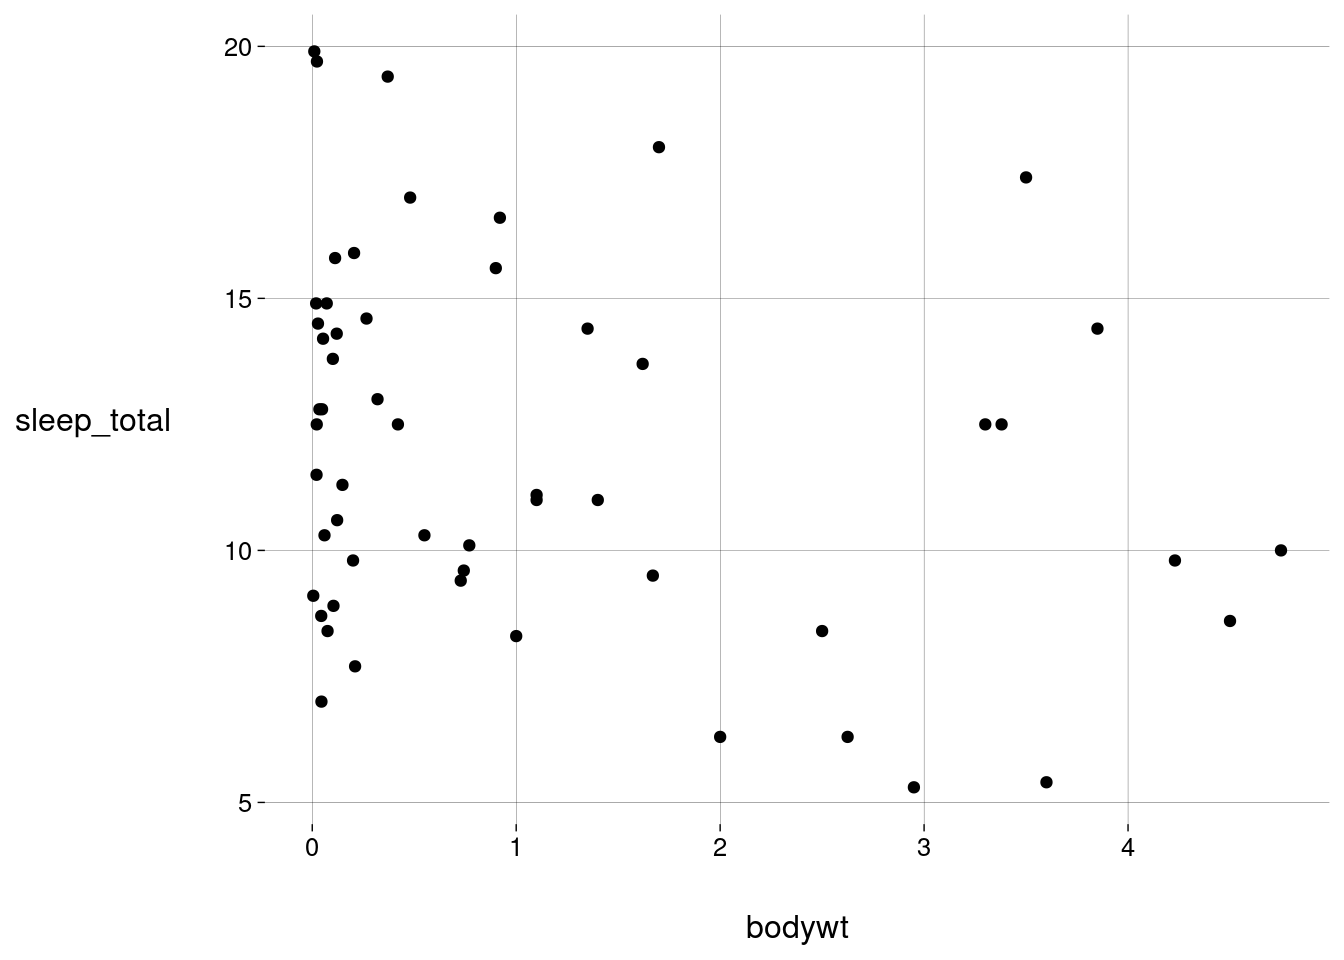
\includegraphics[width=1\linewidth]{_main_files/figure-latex/sono-peso-plot-pequenos-1} \end{center}
\end{itemize}

\hypertarget{incluindo-a-dieta}{%
\subsection{Incluindo a dieta}\label{incluindo-a-dieta}}

\begin{itemize}
\item
  Com a estética \texttt{color}. Observe como a legenda aparece automaticamente.

\begin{Shaded}
\begin{Highlighting}[]
\NormalTok{sono }\SpecialCharTok{\%\textgreater{}\%} 
  \FunctionTok{filter}\NormalTok{(bodywt }\SpecialCharTok{\textless{}}\NormalTok{ limite) }\SpecialCharTok{\%\textgreater{}\%} 
  \FunctionTok{ggplot}\NormalTok{(}\FunctionTok{aes}\NormalTok{(}\AttributeTok{x =}\NormalTok{ bodywt, }\AttributeTok{y =}\NormalTok{ sleep\_total, }\AttributeTok{color =}\NormalTok{ vore)) }\SpecialCharTok{+}
    \FunctionTok{geom\_point}\NormalTok{()}
\end{Highlighting}
\end{Shaded}

  \begin{center}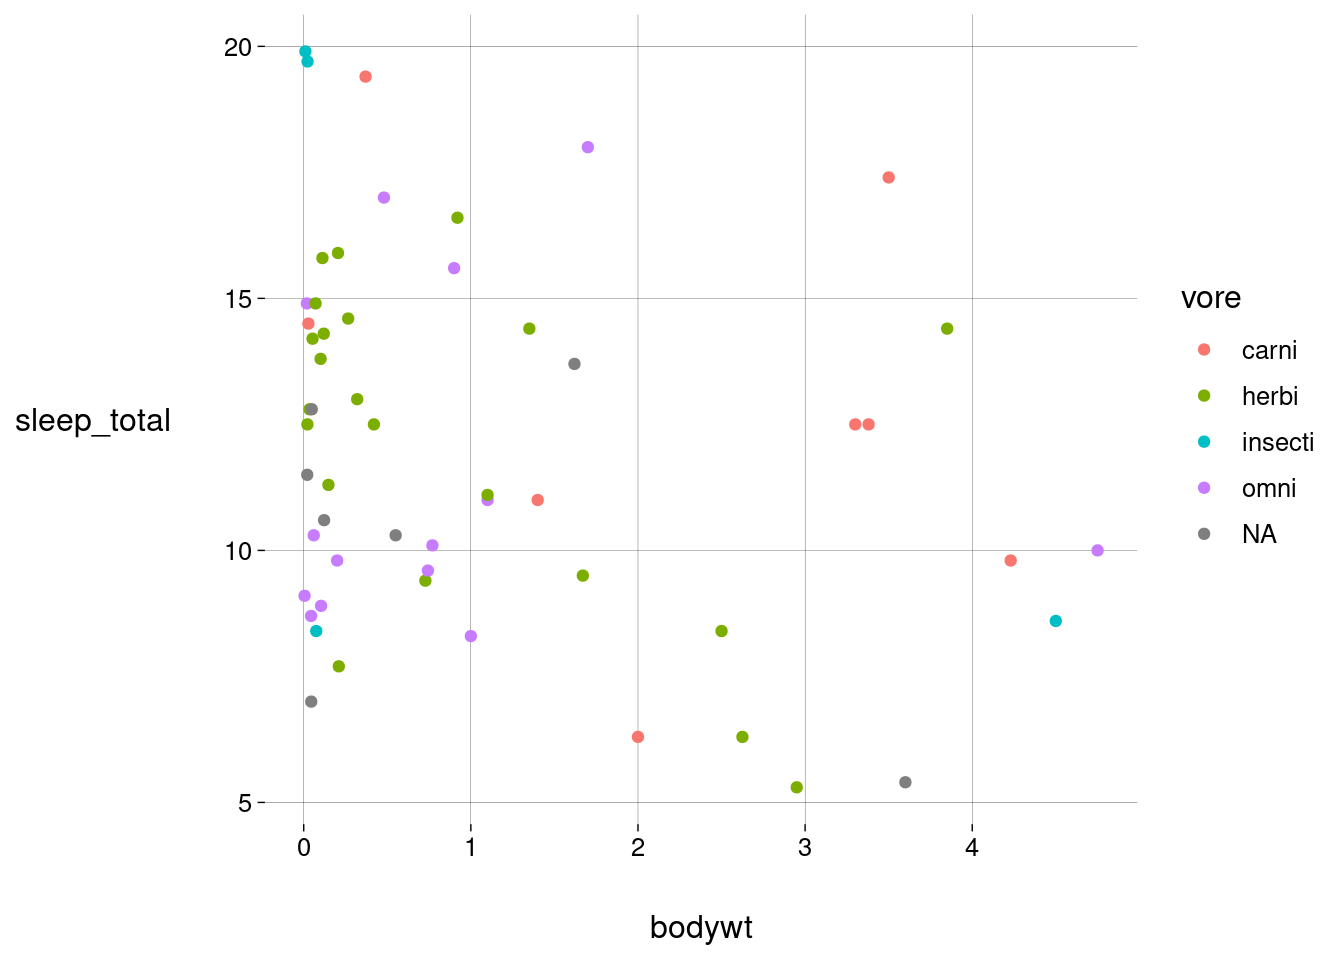
\includegraphics[width=1\linewidth]{_main_files/figure-latex/plot-sono-peso-dieta-1} \end{center}
\end{itemize}

\hypertarget{a-estuxe9tica-pode-ser-especificada-na-geom}{%
\subsection{\texorpdfstring{A estética pode ser especificada na \texttt{geom}}{A estética pode ser especificada na geom}}\label{a-estuxe9tica-pode-ser-especificada-na-geom}}

\begin{itemize}
\item
  Compare com o código anterior.

\begin{Shaded}
\begin{Highlighting}[]
\NormalTok{sono }\SpecialCharTok{\%\textgreater{}\%} 
  \FunctionTok{filter}\NormalTok{(bodywt }\SpecialCharTok{\textless{}}\NormalTok{ limite) }\SpecialCharTok{\%\textgreater{}\%} 
  \FunctionTok{ggplot}\NormalTok{() }\SpecialCharTok{+}
    \FunctionTok{geom\_point}\NormalTok{(}\FunctionTok{aes}\NormalTok{(}\AttributeTok{x =}\NormalTok{ bodywt, }\AttributeTok{y =}\NormalTok{ sleep\_total, }\AttributeTok{color =}\NormalTok{ vore))}
\end{Highlighting}
\end{Shaded}

  \begin{center}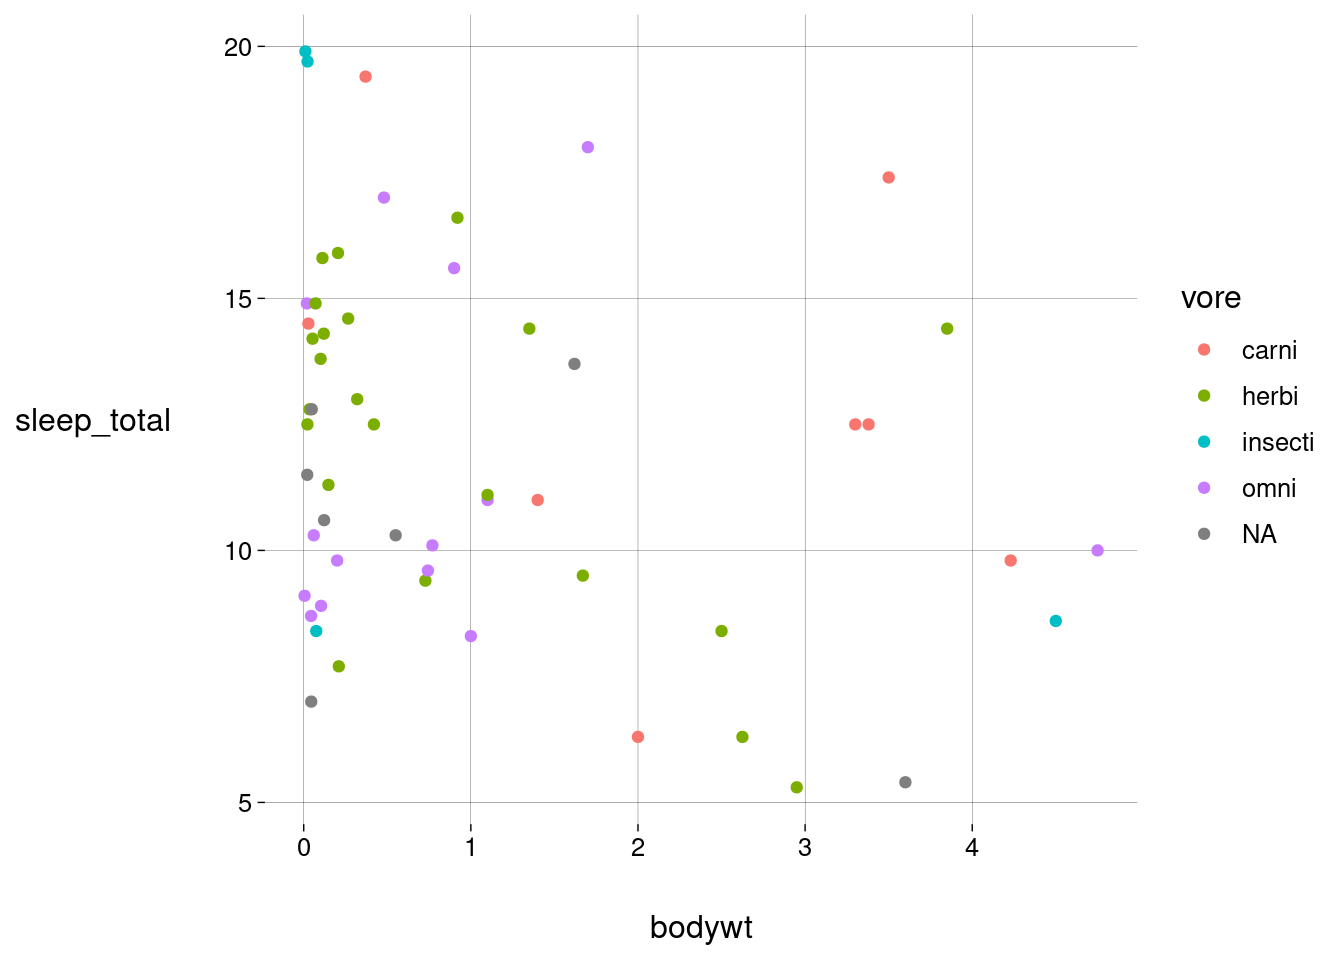
\includegraphics[width=1\linewidth]{_main_files/figure-latex/plot-sono-peso-dieta-geom-1} \end{center}
\item
  Fazendo deste modo, a estética só vale para uma geometria. Se você acrescentar outras geometrias (linhas, por exemplo), a estética não valerá para elas.
\end{itemize}

\hypertarget{aparuxeancia-fixa-ou-dependendo-de-variuxe1vel}{%
\subsection{Aparência fixa ou dependendo de variável?}\label{aparuxeancia-fixa-ou-dependendo-de-variuxe1vel}}

\begin{itemize}
\item
  Se for fixa, não é estética. Não representa informação.
\item
  Se depender de variável, é estética. Representa informação.
\item
  Compare o último \emph{chunk} acima com:

\begin{Shaded}
\begin{Highlighting}[]
\NormalTok{sono }\SpecialCharTok{\%\textgreater{}\%} 
  \FunctionTok{filter}\NormalTok{(bodywt }\SpecialCharTok{\textless{}}\NormalTok{ limite) }\SpecialCharTok{\%\textgreater{}\%} 
  \FunctionTok{ggplot}\NormalTok{() }\SpecialCharTok{+}
    \FunctionTok{geom\_point}\NormalTok{(}\FunctionTok{aes}\NormalTok{(}\AttributeTok{x =}\NormalTok{ bodywt, }\AttributeTok{y =}\NormalTok{ sleep\_total), }\AttributeTok{color =} \StringTok{\textquotesingle{}blue\textquotesingle{}}\NormalTok{)}
\end{Highlighting}
\end{Shaded}

  \begin{center}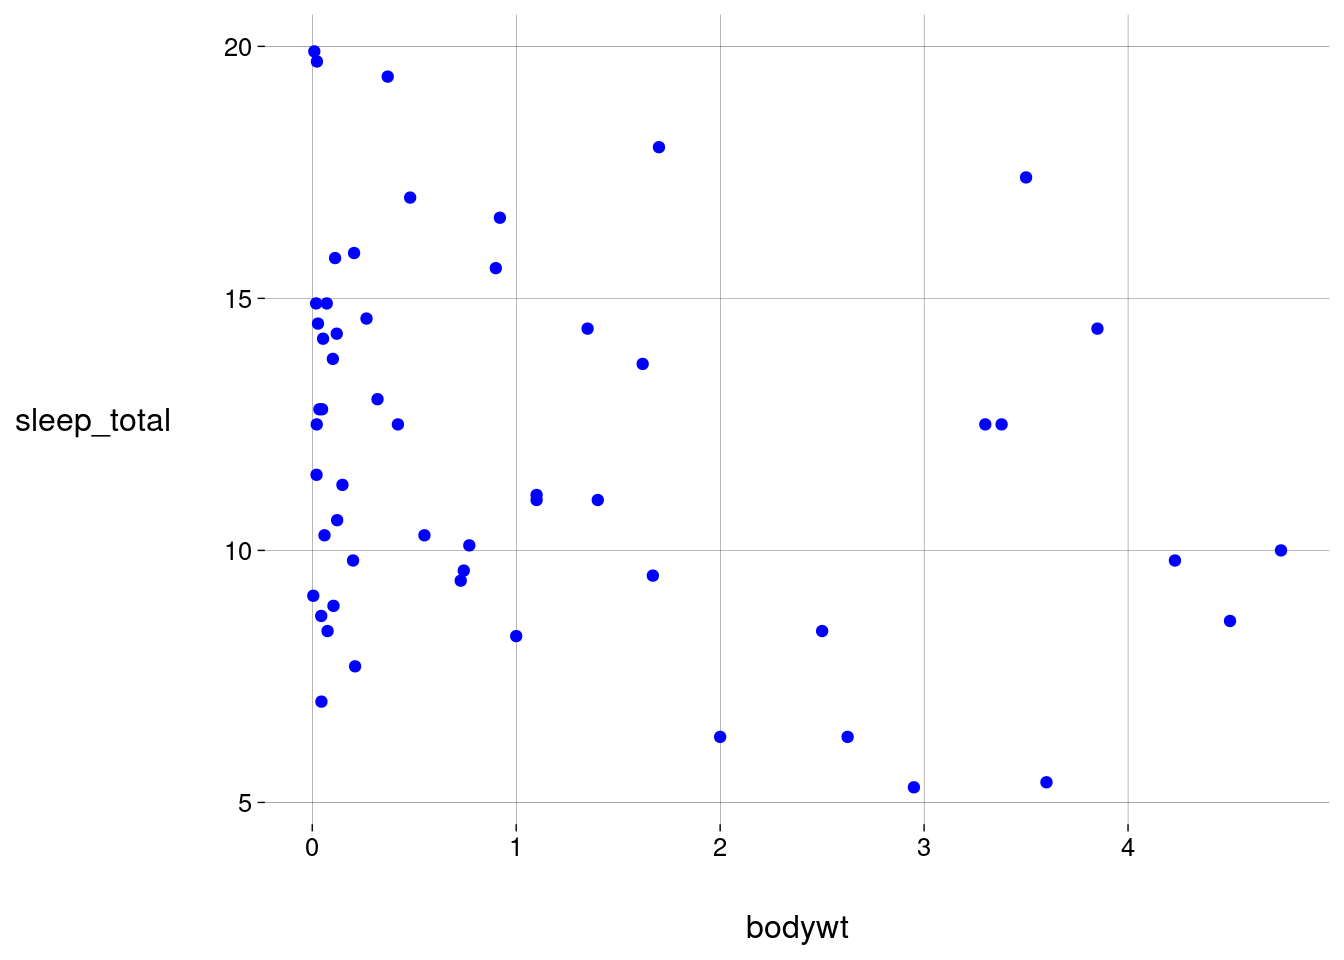
\includegraphics[width=1\linewidth]{_main_files/figure-latex/plot-sono-peso-cor-1} \end{center}
\item
  Se for uma estética, precisa estar {\hl{associada a uma variável}}, não a um valor fixo. Um erro comum seria fazer:

\begin{Shaded}
\begin{Highlighting}[]
\NormalTok{sono }\SpecialCharTok{\%\textgreater{}\%} 
  \FunctionTok{filter}\NormalTok{(bodywt }\SpecialCharTok{\textless{}}\NormalTok{ limite) }\SpecialCharTok{\%\textgreater{}\%} 
  \FunctionTok{ggplot}\NormalTok{() }\SpecialCharTok{+}
    \FunctionTok{geom\_point}\NormalTok{(}\FunctionTok{aes}\NormalTok{(}\AttributeTok{x =}\NormalTok{ bodywt, }\AttributeTok{y =}\NormalTok{ sleep\_total, }\AttributeTok{color =} \StringTok{\textquotesingle{}blue\textquotesingle{}}\NormalTok{))}
\end{Highlighting}
\end{Shaded}

  \begin{center}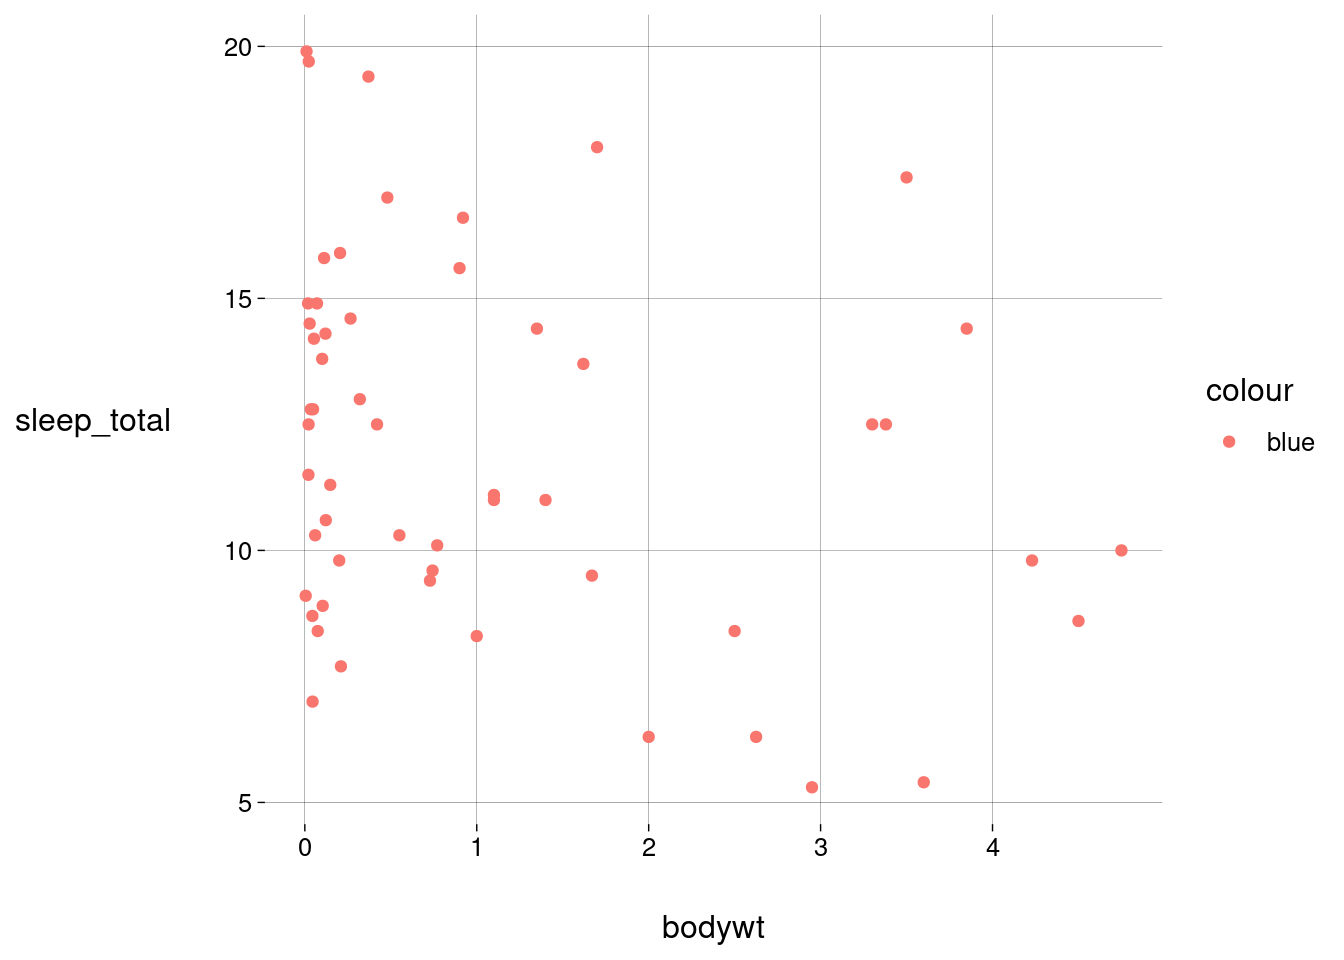
\includegraphics[width=1\linewidth]{_main_files/figure-latex/plot-sono-peso-cor-erro-1} \end{center}
\end{itemize}

\hypertarget{uma-correlauxe7uxe3o-mais-clara}{%
\subsection{Uma correlação mais clara}\label{uma-correlauxe7uxe3o-mais-clara}}

\begin{itemize}
\item
  Peso cerebral versus peso corporal:

\begin{Shaded}
\begin{Highlighting}[]
\NormalTok{sono }\SpecialCharTok{\%\textgreater{}\%} 
  \FunctionTok{ggplot}\NormalTok{(}\FunctionTok{aes}\NormalTok{(}\AttributeTok{x =}\NormalTok{ bodywt, }\AttributeTok{y =}\NormalTok{ brainwt)) }\SpecialCharTok{+}
    \FunctionTok{geom\_point}\NormalTok{()}
\end{Highlighting}
\end{Shaded}

\begin{verbatim}
## Warning: Removed 27 rows containing missing values (geom_point).
\end{verbatim}

  \begin{center}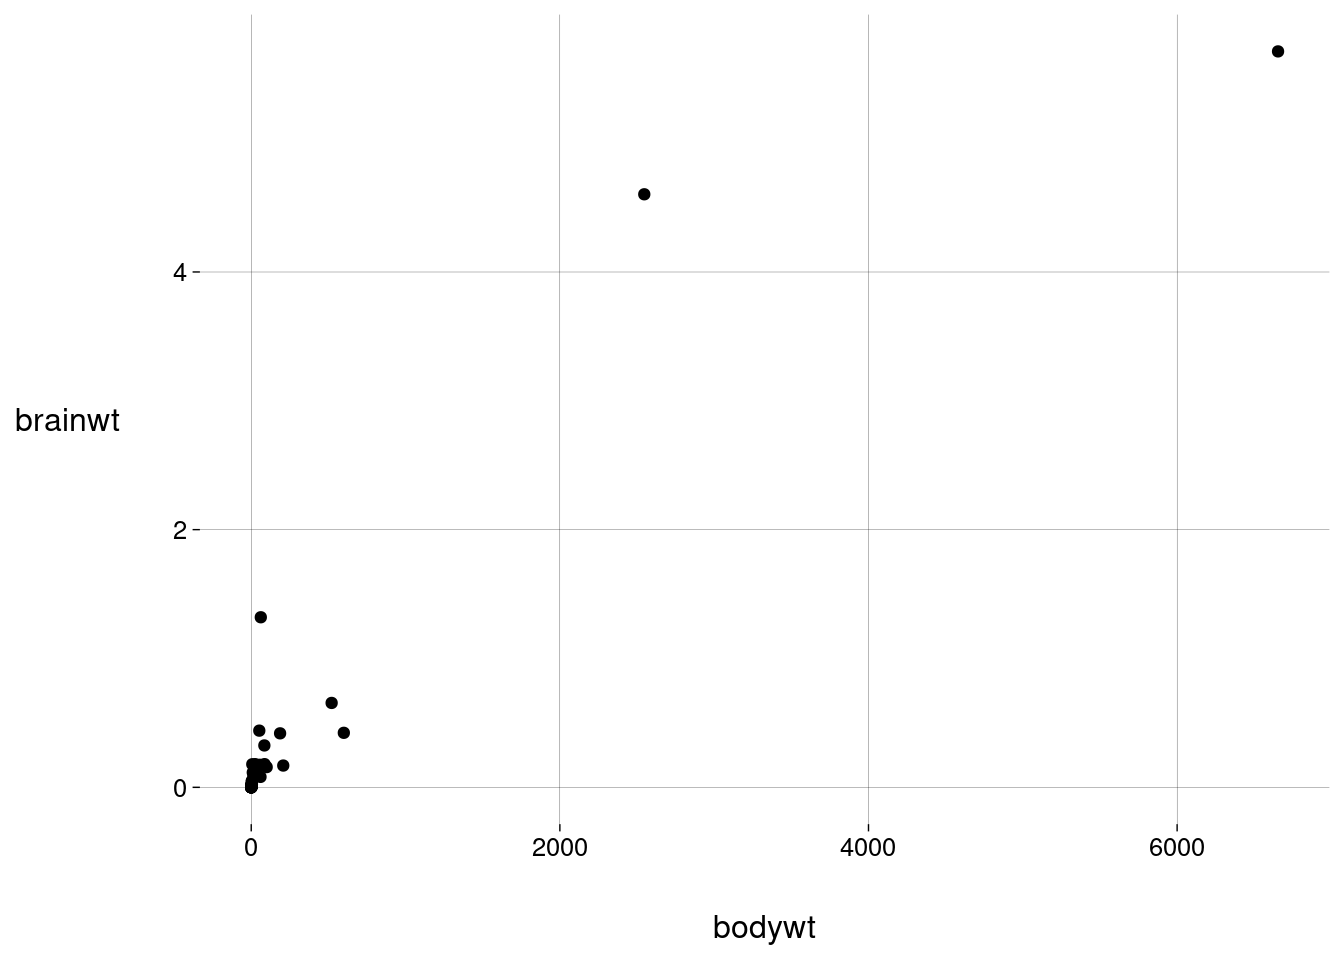
\includegraphics[width=1\linewidth]{_main_files/figure-latex/cerebro-corpo-1} \end{center}
\item
  A mensagem de aviso (\emph{warning}) diz que há $27$ valores faltantes (\texttt{NA}) em \texttt{bodywt} ou \texttt{brainwt}. De fato:

\begin{Shaded}
\begin{Highlighting}[]
\NormalTok{sono }\SpecialCharTok{\%\textgreater{}\%} 
  \FunctionTok{filter}\NormalTok{(}\FunctionTok{is.na}\NormalTok{(bodywt)) }\SpecialCharTok{\%\textgreater{}\%} 
  \FunctionTok{count}\NormalTok{()}
\end{Highlighting}
\end{Shaded}

\begin{verbatim}
## # A tibble: 1 x 1
##       n
##   <int>
## 1     0
\end{verbatim}

\begin{Shaded}
\begin{Highlighting}[]
\NormalTok{sono }\SpecialCharTok{\%\textgreater{}\%} 
  \FunctionTok{filter}\NormalTok{(}\FunctionTok{is.na}\NormalTok{(brainwt)) }\SpecialCharTok{\%\textgreater{}\%} 
  \FunctionTok{count}\NormalTok{()}
\end{Highlighting}
\end{Shaded}

\begin{verbatim}
## # A tibble: 1 x 1
##       n
##   <int>
## 1    27
\end{verbatim}
\item
  Vamos restringir aos animais mais leves e mudar a opacidade:

\begin{Shaded}
\begin{Highlighting}[]
\NormalTok{sono }\SpecialCharTok{\%\textgreater{}\%} 
  \FunctionTok{filter}\NormalTok{(bodywt }\SpecialCharTok{\textless{}}\NormalTok{ limite) }\SpecialCharTok{\%\textgreater{}\%} 
  \FunctionTok{ggplot}\NormalTok{(}\FunctionTok{aes}\NormalTok{(}\AttributeTok{x =}\NormalTok{ bodywt, }\AttributeTok{y =}\NormalTok{ brainwt)) }\SpecialCharTok{+}
    \FunctionTok{geom\_point}\NormalTok{(}\AttributeTok{alpha =}\NormalTok{ .}\DecValTok{5}\NormalTok{)}
\end{Highlighting}
\end{Shaded}

\begin{verbatim}
## Warning: Removed 18 rows containing missing values (geom_point).
\end{verbatim}

  \begin{center}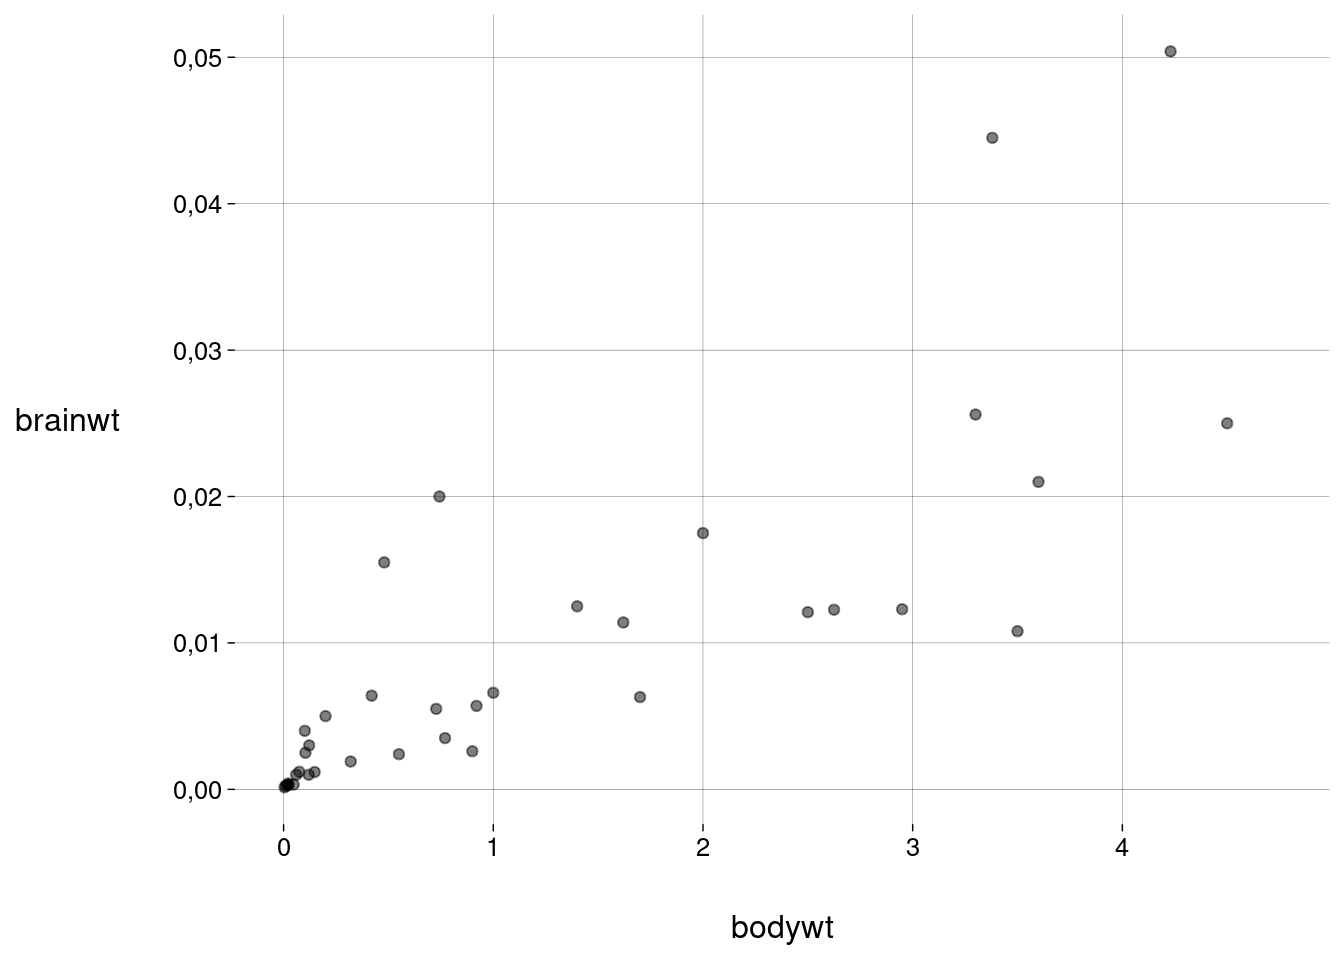
\includegraphics[width=1\linewidth]{_main_files/figure-latex/cerebro-corpo-2-1} \end{center}
\item
  Vamos incluir horas de sono e dieta. Observe as estéticas usadas.

\begin{Shaded}
\begin{Highlighting}[]
\NormalTok{sono }\SpecialCharTok{\%\textgreater{}\%} 
  \FunctionTok{filter}\NormalTok{(bodywt }\SpecialCharTok{\textless{}}\NormalTok{ limite) }\SpecialCharTok{\%\textgreater{}\%} 
  \FunctionTok{ggplot}\NormalTok{(}
    \FunctionTok{aes}\NormalTok{(}
      \AttributeTok{x =}\NormalTok{ bodywt, }
      \AttributeTok{y =}\NormalTok{ brainwt,}
      \AttributeTok{size =}\NormalTok{ sleep\_total,}
      \AttributeTok{color =}\NormalTok{ vore}
\NormalTok{    )}
\NormalTok{  ) }\SpecialCharTok{+}
    \FunctionTok{geom\_point}\NormalTok{(}\AttributeTok{alpha =}\NormalTok{ .}\DecValTok{5}\NormalTok{)}
\end{Highlighting}
\end{Shaded}

\begin{verbatim}
## Warning: Removed 18 rows containing missing values (geom_point).
\end{verbatim}

  \begin{center}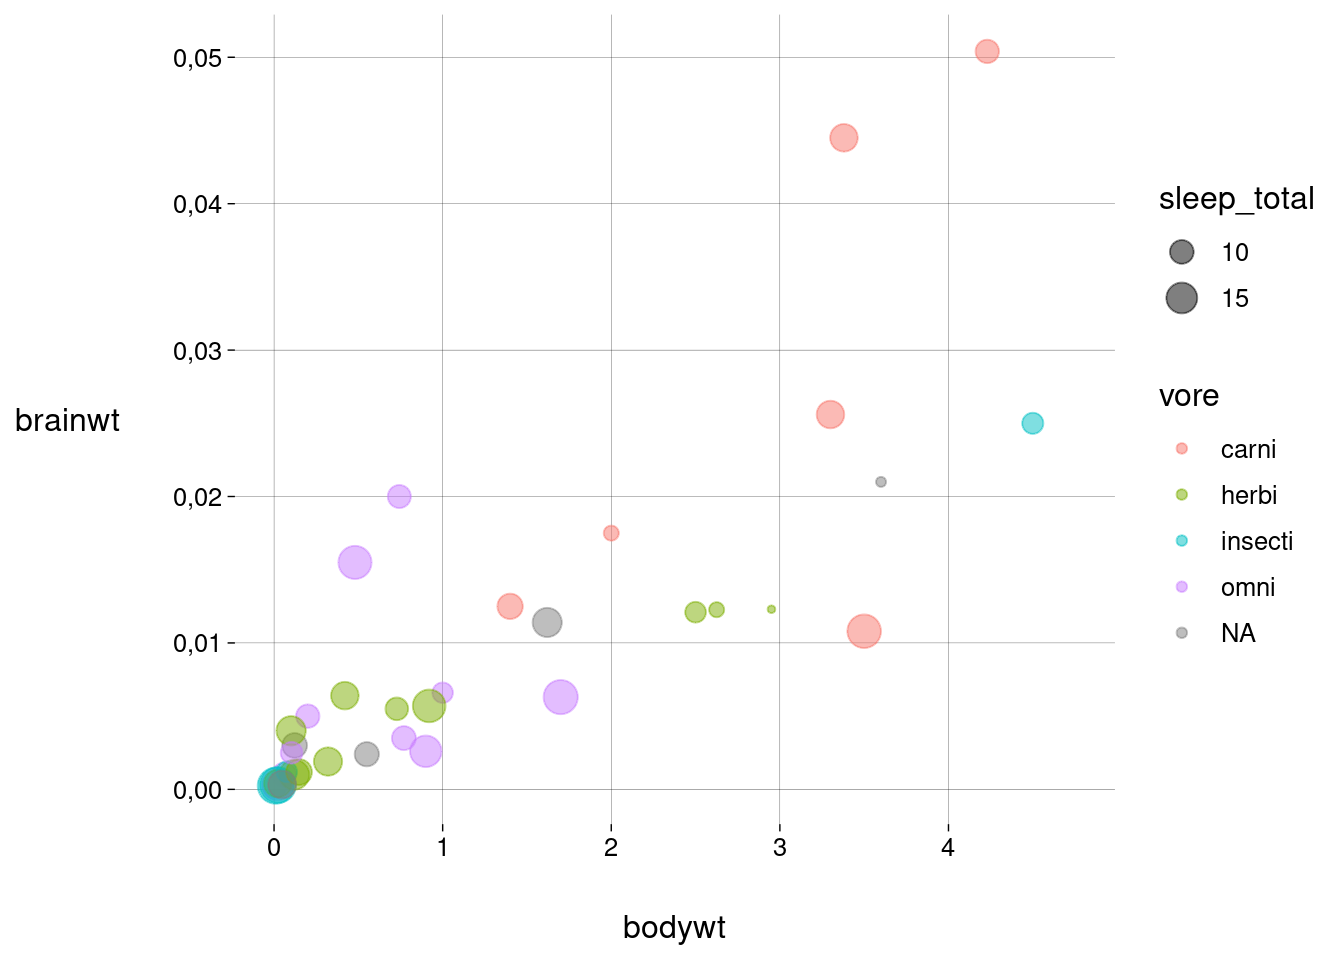
\includegraphics[width=1\linewidth]{_main_files/figure-latex/cerebro-corpo-3-1} \end{center}
\item
  Vamos mudar a escala dos tamanhos e incluir rótulos:

\begin{Shaded}
\begin{Highlighting}[]
\NormalTok{grafico }\OtherTok{\textless{}{-}}\NormalTok{ sono }\SpecialCharTok{\%\textgreater{}\%} 
  \FunctionTok{filter}\NormalTok{(bodywt }\SpecialCharTok{\textless{}}\NormalTok{ limite) }\SpecialCharTok{\%\textgreater{}\%} 
  \FunctionTok{ggplot}\NormalTok{(}
    \FunctionTok{aes}\NormalTok{(}
      \AttributeTok{x =}\NormalTok{ bodywt, }
      \AttributeTok{y =}\NormalTok{ brainwt,}
      \AttributeTok{size =}\NormalTok{ sleep\_total,}
      \AttributeTok{color =}\NormalTok{ vore}
\NormalTok{    )}
\NormalTok{  ) }\SpecialCharTok{+}
    \FunctionTok{geom\_point}\NormalTok{(}\AttributeTok{alpha =}\NormalTok{ .}\DecValTok{5}\NormalTok{) }\SpecialCharTok{+}
    \FunctionTok{scale\_size}\NormalTok{(}
      \AttributeTok{breaks =} \FunctionTok{seq}\NormalTok{(}\DecValTok{0}\NormalTok{, }\DecValTok{24}\NormalTok{, }\DecValTok{4}\NormalTok{)}
\NormalTok{    ) }\SpecialCharTok{+}
    \FunctionTok{labs}\NormalTok{(}
      \AttributeTok{title =} \StringTok{\textquotesingle{}Peso do cérebro versus peso corporal\textquotesingle{}}\NormalTok{,}
      \AttributeTok{subtitle =} \FunctionTok{paste0}\NormalTok{(}
        \StringTok{\textquotesingle{}para mamíferos com menos de \textquotesingle{}}\NormalTok{, }
\NormalTok{        limite, }
        \StringTok{\textquotesingle{} kg\textquotesingle{}}
\NormalTok{      ),}
      \AttributeTok{caption =} \StringTok{\textquotesingle{}Fonte: dataset \textasciigrave{}msleep\textasciigrave{}\textquotesingle{}}\NormalTok{,}
      \AttributeTok{x =} \StringTok{\textquotesingle{}Peso corporal (kg)\textquotesingle{}}\NormalTok{,}
      \AttributeTok{y =} \StringTok{\textquotesingle{}Peso do}\SpecialCharTok{\textbackslash{}n}\StringTok{ cérebro (kg)\textquotesingle{}}\NormalTok{,}
      \AttributeTok{color =} \StringTok{\textquotesingle{}Dieta\textquotesingle{}}\NormalTok{,}
      \AttributeTok{size =} \StringTok{\textquotesingle{}Horas}\SpecialCharTok{\textbackslash{}n}\StringTok{de sono\textquotesingle{}}
\NormalTok{    )}

\NormalTok{grafico}
\end{Highlighting}
\end{Shaded}

\begin{verbatim}
## Warning: Removed 18 rows containing missing values (geom_point).
\end{verbatim}

  \begin{center}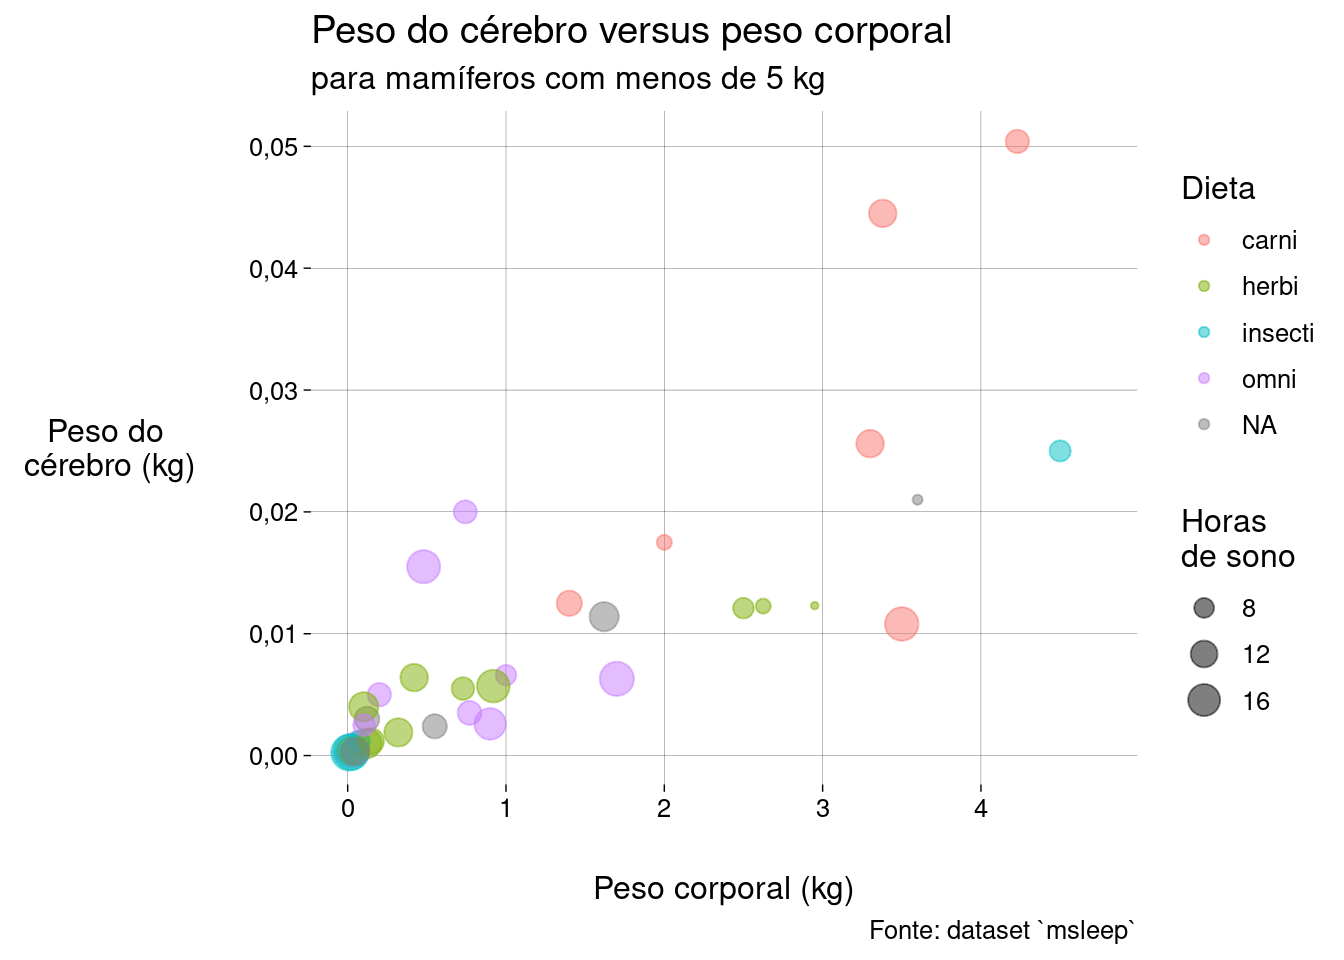
\includegraphics[width=1\linewidth]{_main_files/figure-latex/cerebro-corpo-4-1} \end{center}
\item
  Vamos mudar as cores usadas para a dieta, usando uma escala diferente.

\begin{Shaded}
\begin{Highlighting}[]
\NormalTok{grafico2 }\OtherTok{\textless{}{-}}\NormalTok{ grafico }\SpecialCharTok{+}
  \FunctionTok{scale\_color\_discrete}\NormalTok{(}
    \AttributeTok{palette =} \StringTok{\textquotesingle{}RdBu\textquotesingle{}}\NormalTok{,}
    \AttributeTok{na.value =} \StringTok{\textquotesingle{}black\textquotesingle{}}\NormalTok{,}
    \AttributeTok{type =}\NormalTok{ scale\_color\_brewer}
\NormalTok{  )}

\NormalTok{grafico2}
\end{Highlighting}
\end{Shaded}

\begin{verbatim}
## Warning: Removed 18 rows containing missing values (geom_point).
\end{verbatim}

  \begin{center}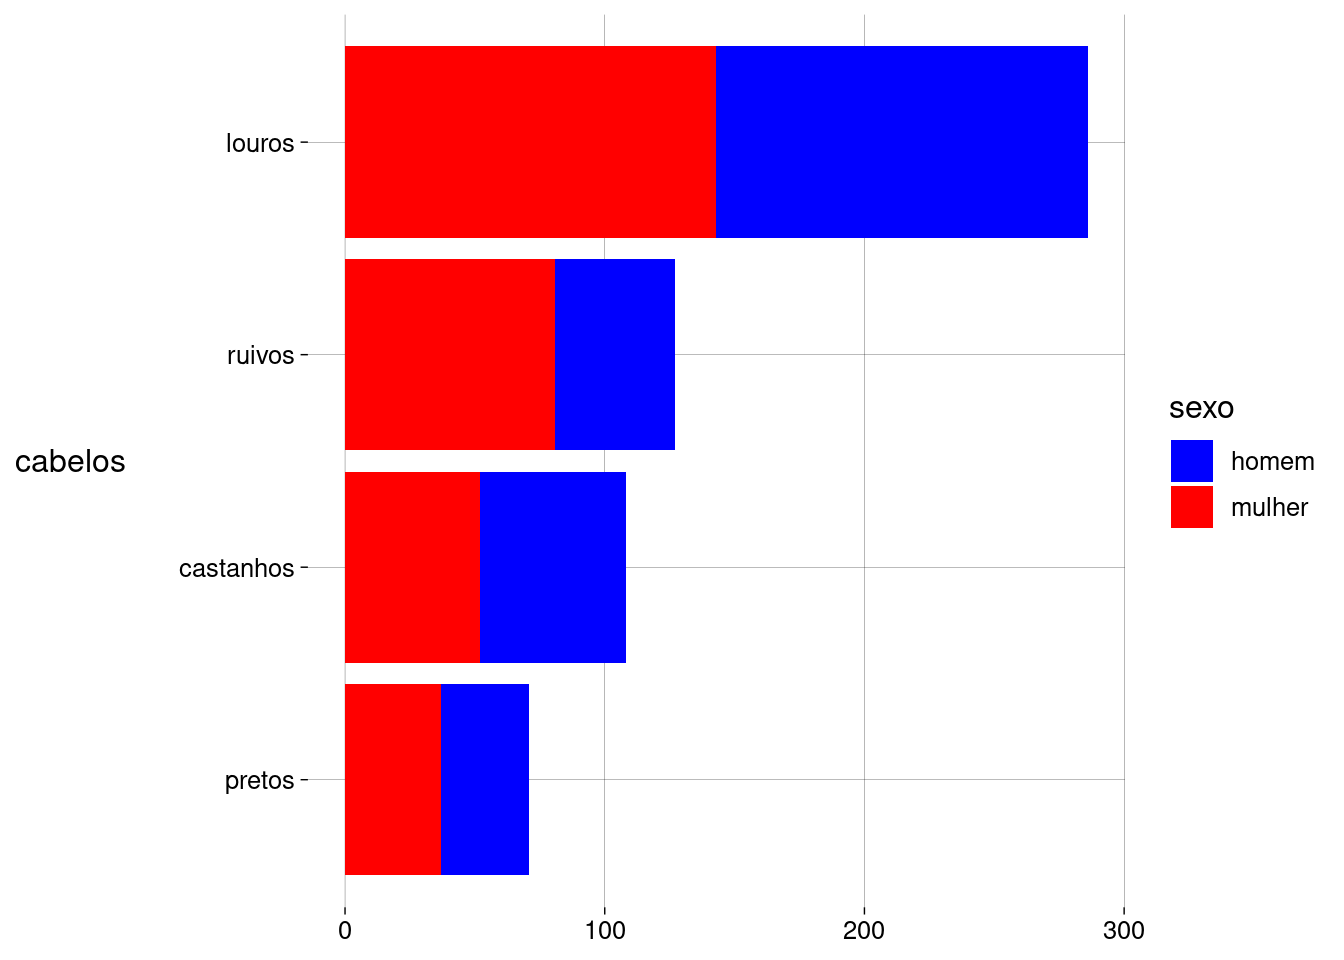
\includegraphics[width=1\linewidth]{_main_files/figure-latex/unnamed-chunk-74-1} \end{center}
\item
  Observe como usamos o gráfico já salvo na variável \texttt{grafico} e simplesmente acrescentamos a nova escala. Este tipo de ``montagem'' de gráficos \texttt{ggplot2} é bem conveniente, para evitar repetição de código.
\item
  Um último ajuste na aparência: os pontos na legenda ``Dieta'' estão pequenos demais. Quase não identificamos as cores deles.

  Vamos usar a função \texttt{guides} para modificar (\emph{override}) a estética \texttt{color} --- {\hl{apenas na legenda, não nos pontos mostrados no gráfico, cujos tamanhos representam o número de horas de sono}} --- tornando o tamanho maior. \href{https://ggplot2-book.org/scale-colour.html\#guide_legend}{Leia mais sobre \texttt{override.aes} neste \emph{link} (em inglês)}.

\begin{Shaded}
\begin{Highlighting}[]
\NormalTok{grafico3 }\OtherTok{\textless{}{-}}\NormalTok{ grafico2 }\SpecialCharTok{+}
  \FunctionTok{guides}\NormalTok{(}\AttributeTok{color =} \FunctionTok{guide\_legend}\NormalTok{(}\AttributeTok{override.aes =} \FunctionTok{list}\NormalTok{(}\AttributeTok{size =} \DecValTok{10}\NormalTok{)))}

\NormalTok{grafico3}
\end{Highlighting}
\end{Shaded}

\begin{verbatim}
## Warning: Removed 18 rows containing missing values (geom_point).
\end{verbatim}

  \begin{center}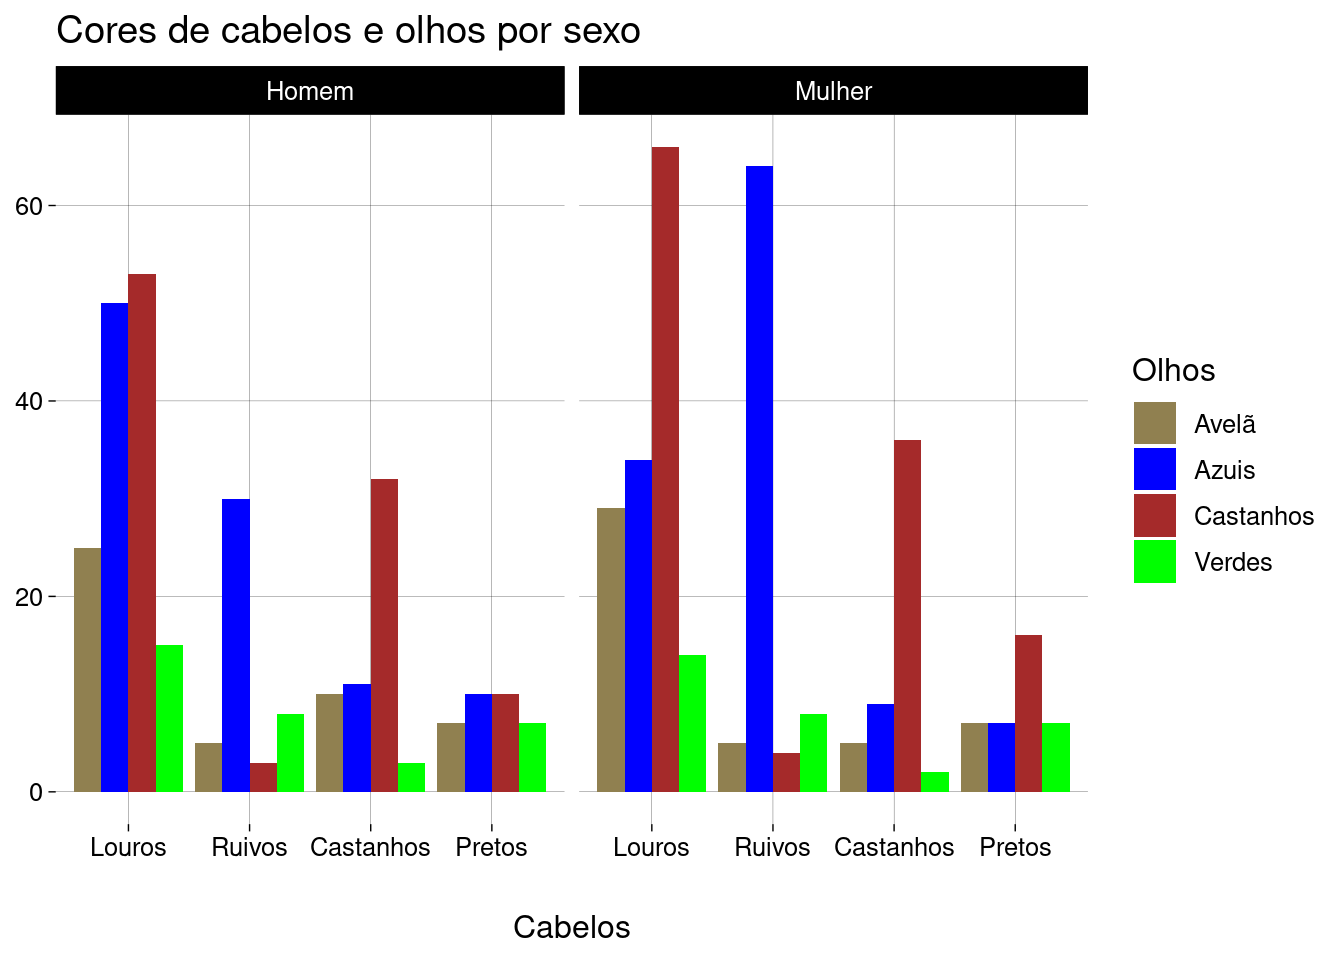
\includegraphics[width=1\linewidth]{_main_files/figure-latex/unnamed-chunk-75-1} \end{center}
\item
  Agora podemos finalmente comentar sobre a informação que o gráfico mostra sobre os dados:

  \begin{itemize}
  \item
    De fato, existe uma correlação entre peso cerebral e peso corporal: quanto maior o peso corporal, maior o peso cerebral. Nada surprenndente.
  \item
    \protect\hypertarget{grafico4}{}{} Podemos fazer o \texttt{ggplot2} traçar uma reta de regressão com a geometria \texttt{geom\_smooth}. Vamos falar mais sobre correlação \protect\hyperlink{correlacao}{em um capítulo futuro}.

\begin{Shaded}
\begin{Highlighting}[]
\NormalTok{grafico4 }\OtherTok{\textless{}{-}}\NormalTok{ grafico3 }\SpecialCharTok{+}
  \FunctionTok{geom\_smooth}\NormalTok{(}
    \FunctionTok{aes}\NormalTok{(}\AttributeTok{group =} \DecValTok{1}\NormalTok{), }
    \AttributeTok{show.legend =} \ConstantTok{FALSE}\NormalTok{,}
    \AttributeTok{method =} \StringTok{\textquotesingle{}lm\textquotesingle{}}\NormalTok{, }
    \AttributeTok{se =} \ConstantTok{FALSE}
\NormalTok{  )}

\NormalTok{grafico4}
\end{Highlighting}
\end{Shaded}

\begin{verbatim}
## `geom_smooth()` using formula 'y ~ x'
\end{verbatim}

\begin{verbatim}
## Warning: Removed 18 rows containing non-finite values (stat_smooth).
\end{verbatim}

\begin{verbatim}
## Warning: Removed 18 rows containing missing values (geom_point).
\end{verbatim}

    \begin{center}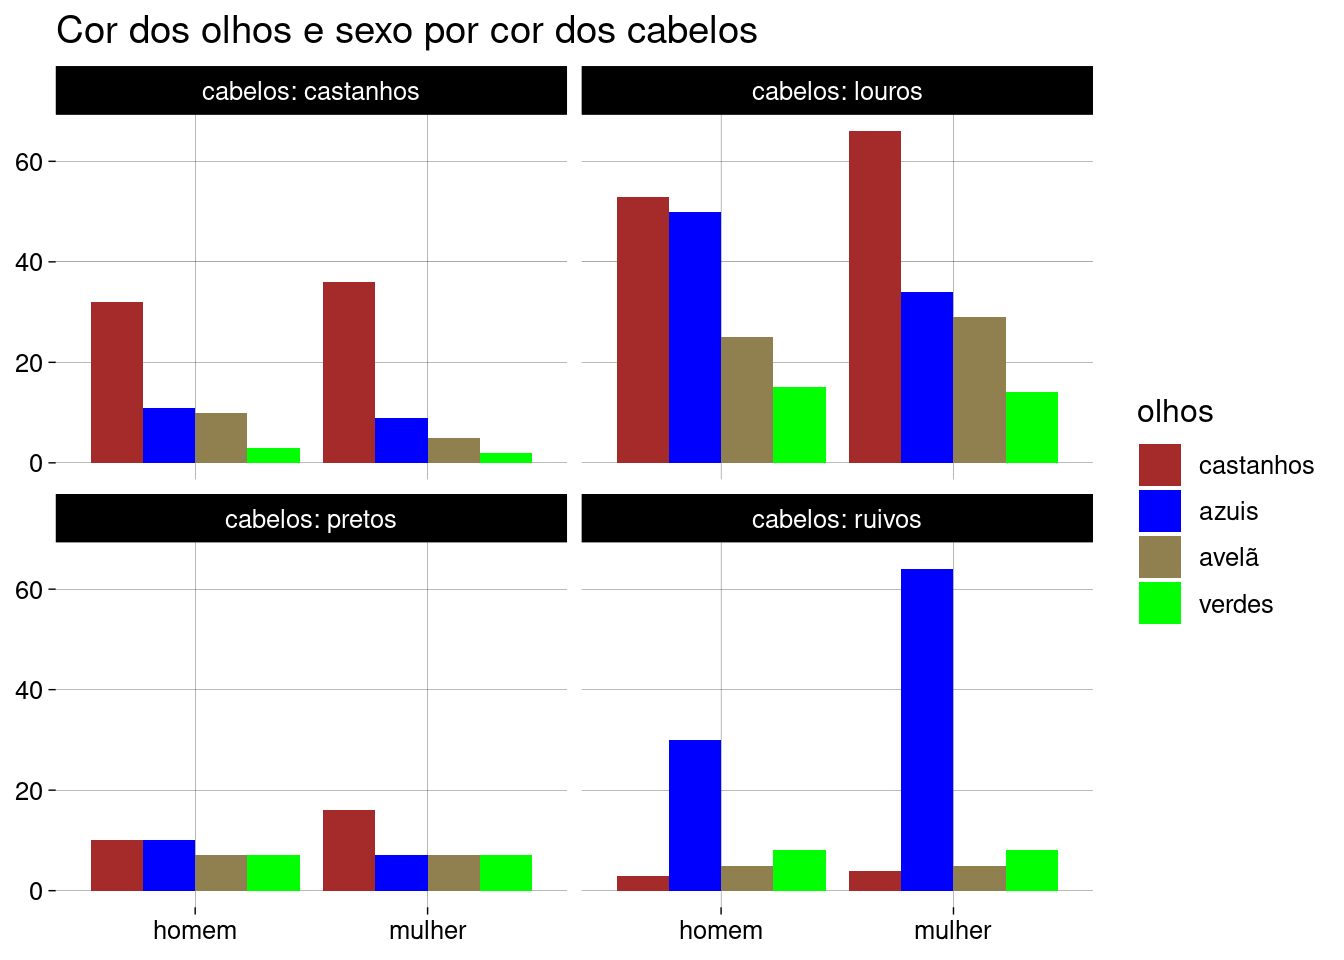
\includegraphics[width=1\linewidth]{_main_files/figure-latex/unnamed-chunk-76-1} \end{center}
  \item
    Todos os carnívoros têm peso corporal maior que $1$kg e peso cerebral maior ou igual a $10$g.
  \item
    Só um carnívoro dorme $8$ horas ou menos. Qual?
  \item
    Todos os insetívoros --- com exceção de um (qual?) --- são muito leves e dormem muito.
  \item
    Todos os onívoros têm menos de $2$kg de peso corporal e $20$g ou menos de peso cerebral.
  \end{itemize}
\end{itemize}

\hypertarget{vuxeddeo-2-1}{%
\section{Vídeo 2}\label{vuxeddeo-2-1}}

\begin{center} \url{https://youtu.be/c-LoZ9e8xWc} \end{center}

\hypertarget{histogramas-e-cia.}{%
\section{Histogramas e cia.}\label{histogramas-e-cia.}}

\begin{itemize}
\tightlist
\item
  A idéia agora é {\hl{agrupar indivíduos em classes,}} dependendo do valor de uma variável quantitativa.
\end{itemize}

\hypertarget{distribuiuxe7uxf5es-de-frequuxeancia}{%
\subsection{Distribuições de frequência}\label{distribuiuxe7uxf5es-de-frequuxeancia}}

\begin{itemize}
\item
  Vamos nos concentrar nas horas de sono.

\begin{Shaded}
\begin{Highlighting}[]
\NormalTok{sono}\SpecialCharTok{$}\NormalTok{sleep\_total}
\end{Highlighting}
\end{Shaded}

\begin{verbatim}
##  [1] 12,1 17,0 14,4 14,9  4,0 14,4  8,7  7,0 10,1  3,0  5,3  9,4 10,0
## [14] 12,5 10,3  8,3  9,1 17,4  5,3 18,0  3,9 19,7  2,9  3,1 10,1 10,9
## [27] 14,9 12,5  9,8  1,9  2,7  6,2  6,3  8,0  9,5  3,3 19,4 10,1 14,2
## [40] 14,3 12,8 12,5 19,9 14,6 11,0  7,7 14,5  8,4  3,8  9,7 15,8 10,4
## [53] 13,5  9,4 10,3 11,0 11,5 13,7  3,5  5,6 11,1 18,1  5,4 13,0  8,7
## [66]  9,6  8,4 11,3 10,6 16,6 13,8 15,9 12,8  9,1  8,6 15,8  4,4 15,6
## [79]  8,9  5,2  6,3 12,5  9,8
\end{verbatim}
\item
  Antes de montar o histograma, vamos construir uma {\hl{distribuição de frequência.}}
\item
  A {\hl{amplitude}} é a diferença entre o valor máximo e o valor mínimo. A função \texttt{range} não retorna a amplitude, mas sim os valores mínimo e máximo:

\begin{Shaded}
\begin{Highlighting}[]
\NormalTok{sono}\SpecialCharTok{$}\NormalTok{sleep\_total }\SpecialCharTok{\%\textgreater{}\%} \FunctionTok{range}\NormalTok{()}
\end{Highlighting}
\end{Shaded}

\begin{verbatim}
## [1]  1,9 19,9
\end{verbatim}
\item
  Vamos decidir que cada classe vai ter $2$ horas. A função \texttt{cut} substitui os valores do vetor pelos nomes das classes:

\begin{Shaded}
\begin{Highlighting}[]
\NormalTok{sono}\SpecialCharTok{$}\NormalTok{sleep\_total }\SpecialCharTok{\%\textgreater{}\%} 
  \FunctionTok{cut}\NormalTok{(}\AttributeTok{breaks =} \FunctionTok{seq}\NormalTok{(}\DecValTok{0}\NormalTok{, }\DecValTok{20}\NormalTok{, }\DecValTok{2}\NormalTok{), }\AttributeTok{right =} \ConstantTok{FALSE}\NormalTok{)}
\end{Highlighting}
\end{Shaded}

\begin{verbatim}
##  [1] [12,14) [16,18) [14,16) [14,16) [4,6)   [14,16) [8,10)  [6,8)  
##  [9] [10,12) [2,4)   [4,6)   [8,10)  [10,12) [12,14) [10,12) [8,10) 
## [17] [8,10)  [16,18) [4,6)   [18,20) [2,4)   [18,20) [2,4)   [2,4)  
## [25] [10,12) [10,12) [14,16) [12,14) [8,10)  [0,2)   [2,4)   [6,8)  
## [33] [6,8)   [8,10)  [8,10)  [2,4)   [18,20) [10,12) [14,16) [14,16)
## [41] [12,14) [12,14) [18,20) [14,16) [10,12) [6,8)   [14,16) [8,10) 
## [49] [2,4)   [8,10)  [14,16) [10,12) [12,14) [8,10)  [10,12) [10,12)
## [57] [10,12) [12,14) [2,4)   [4,6)   [10,12) [18,20) [4,6)   [12,14)
## [65] [8,10)  [8,10)  [8,10)  [10,12) [10,12) [16,18) [12,14) [14,16)
## [73] [12,14) [8,10)  [8,10)  [14,16) [4,6)   [14,16) [8,10)  [4,6)  
## [81] [6,8)   [12,14) [8,10) 
## 10 Levels: [0,2) [2,4) [4,6) [6,8) [8,10) [10,12) [12,14) ... [18,20)
\end{verbatim}
\item
  A função \texttt{table} faz a contagem dos elementos de cada classe:

\begin{Shaded}
\begin{Highlighting}[]
\NormalTok{sono}\SpecialCharTok{$}\NormalTok{sleep\_total }\SpecialCharTok{\%\textgreater{}\%}  
  \FunctionTok{cut}\NormalTok{(}\AttributeTok{breaks =} \FunctionTok{seq}\NormalTok{(}\DecValTok{0}\NormalTok{, }\DecValTok{20}\NormalTok{, }\DecValTok{2}\NormalTok{), }\AttributeTok{right =} \ConstantTok{FALSE}\NormalTok{) }\SpecialCharTok{\%\textgreater{}\%} 
  \FunctionTok{table}\NormalTok{(}\AttributeTok{dnn =} \StringTok{\textquotesingle{}Horas de sono\textquotesingle{}}\NormalTok{) }\SpecialCharTok{\%\textgreater{}\%} 
  \FunctionTok{as.data.frame}\NormalTok{()}
\end{Highlighting}
\end{Shaded}

\begin{verbatim}
## # A tibble: 10 x 2
##   Horas.de.sono  Freq
##   <fct>         <int>
## 1 [0,2)             1
## 2 [2,4)             8
## 3 [4,6)             7
## 4 [6,8)             5
## 5 [8,10)           17
## 6 [10,12)          14
## # ... with 4 more rows
\end{verbatim}
\end{itemize}

\hypertarget{histograma}{%
\subsection{Histograma}\label{histograma}}

\begin{itemize}
\item
  Na verdade, o \texttt{ggplot2} já faz esses cálculos para nós.
\item
  O \emph{default} é criar $30$ classes (\emph{bins}):

\begin{Shaded}
\begin{Highlighting}[]
\NormalTok{sono }\SpecialCharTok{\%\textgreater{}\%} 
  \FunctionTok{ggplot}\NormalTok{(}\FunctionTok{aes}\NormalTok{(}\AttributeTok{x =}\NormalTok{ sleep\_total)) }\SpecialCharTok{+}
    \FunctionTok{geom\_histogram}\NormalTok{()}
\end{Highlighting}
\end{Shaded}

\begin{verbatim}
## `stat_bin()` using `bins = 30`. Pick better value with `binwidth`.
\end{verbatim}

  \begin{center}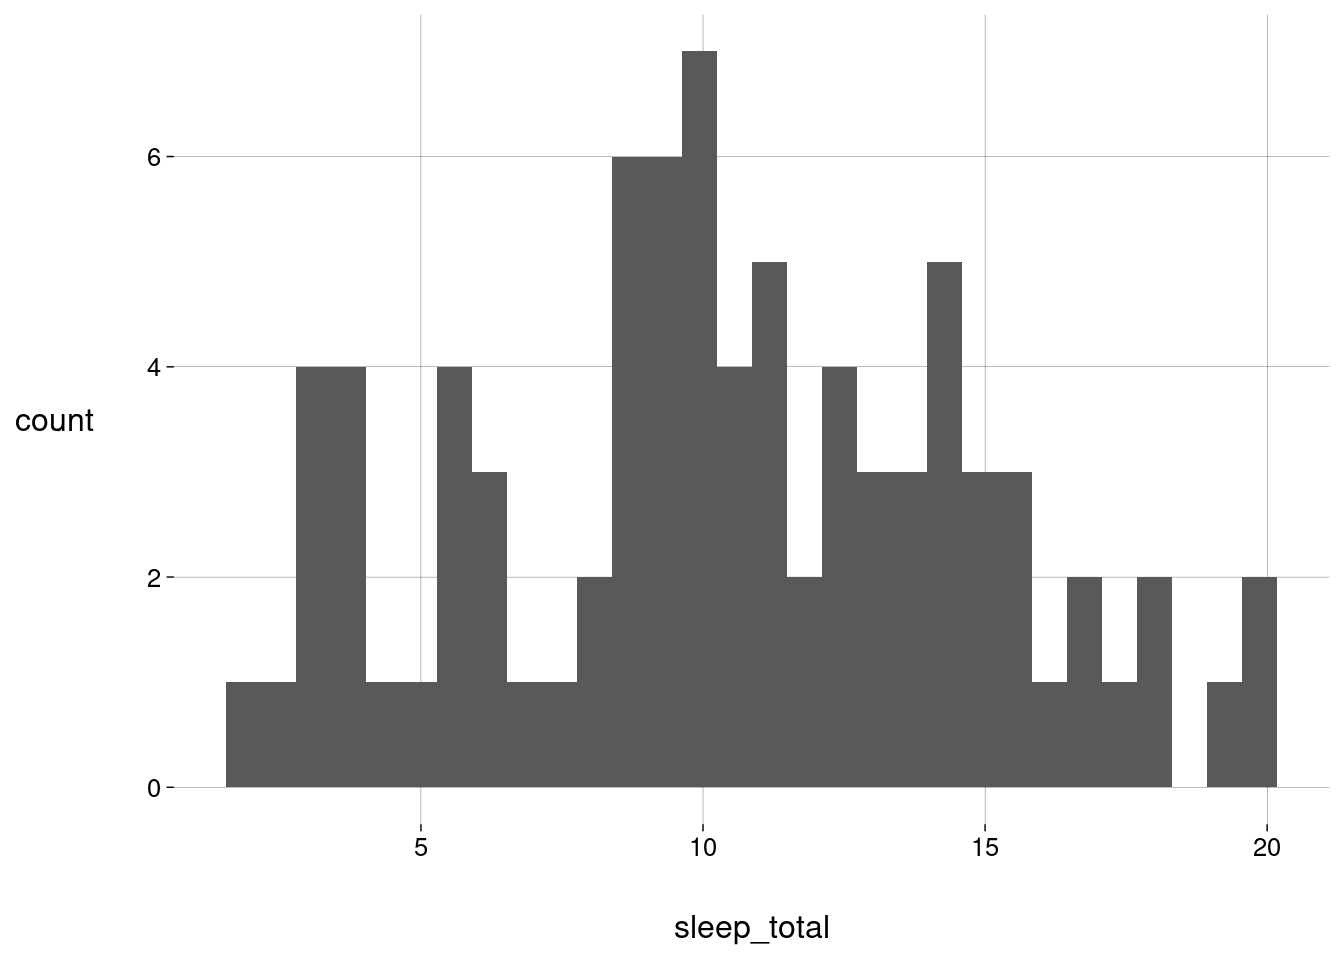
\includegraphics[width=1\linewidth]{_main_files/figure-latex/hist-sono1-1} \end{center}
\item
  \protect\hypertarget{histograma1}{}{} Vamos mudar isto passando um vetor de limites das classes (\emph{breaks}). Vamos acrescentar rótulos também:

\begin{Shaded}
\begin{Highlighting}[]
\NormalTok{sono }\SpecialCharTok{\%\textgreater{}\%} 
  \FunctionTok{ggplot}\NormalTok{(}\FunctionTok{aes}\NormalTok{(}\AttributeTok{x =}\NormalTok{ sleep\_total)) }\SpecialCharTok{+}
    \FunctionTok{geom\_histogram}\NormalTok{(}\AttributeTok{breaks =} \FunctionTok{seq}\NormalTok{(}\DecValTok{0}\NormalTok{, }\DecValTok{20}\NormalTok{, }\DecValTok{2}\NormalTok{)) }\SpecialCharTok{+}
    \FunctionTok{scale\_x\_continuous}\NormalTok{(}\AttributeTok{breaks =} \FunctionTok{seq}\NormalTok{(}\DecValTok{0}\NormalTok{, }\DecValTok{20}\NormalTok{, }\DecValTok{2}\NormalTok{)) }\SpecialCharTok{+}
    \FunctionTok{labs}\NormalTok{(}
      \AttributeTok{title =} \StringTok{\textquotesingle{}Horas de sono de diversos mamíferos\textquotesingle{}}\NormalTok{,}
      \AttributeTok{x =} \StringTok{\textquotesingle{}horas de sono\textquotesingle{}}\NormalTok{,}
      \AttributeTok{y =} \ConstantTok{NULL}\NormalTok{,}
      \AttributeTok{caption =} \StringTok{\textquotesingle{}Fonte: dataset \textasciigrave{}msleep\textasciigrave{}\textquotesingle{}}
\NormalTok{    )}
\end{Highlighting}
\end{Shaded}

  \begin{center}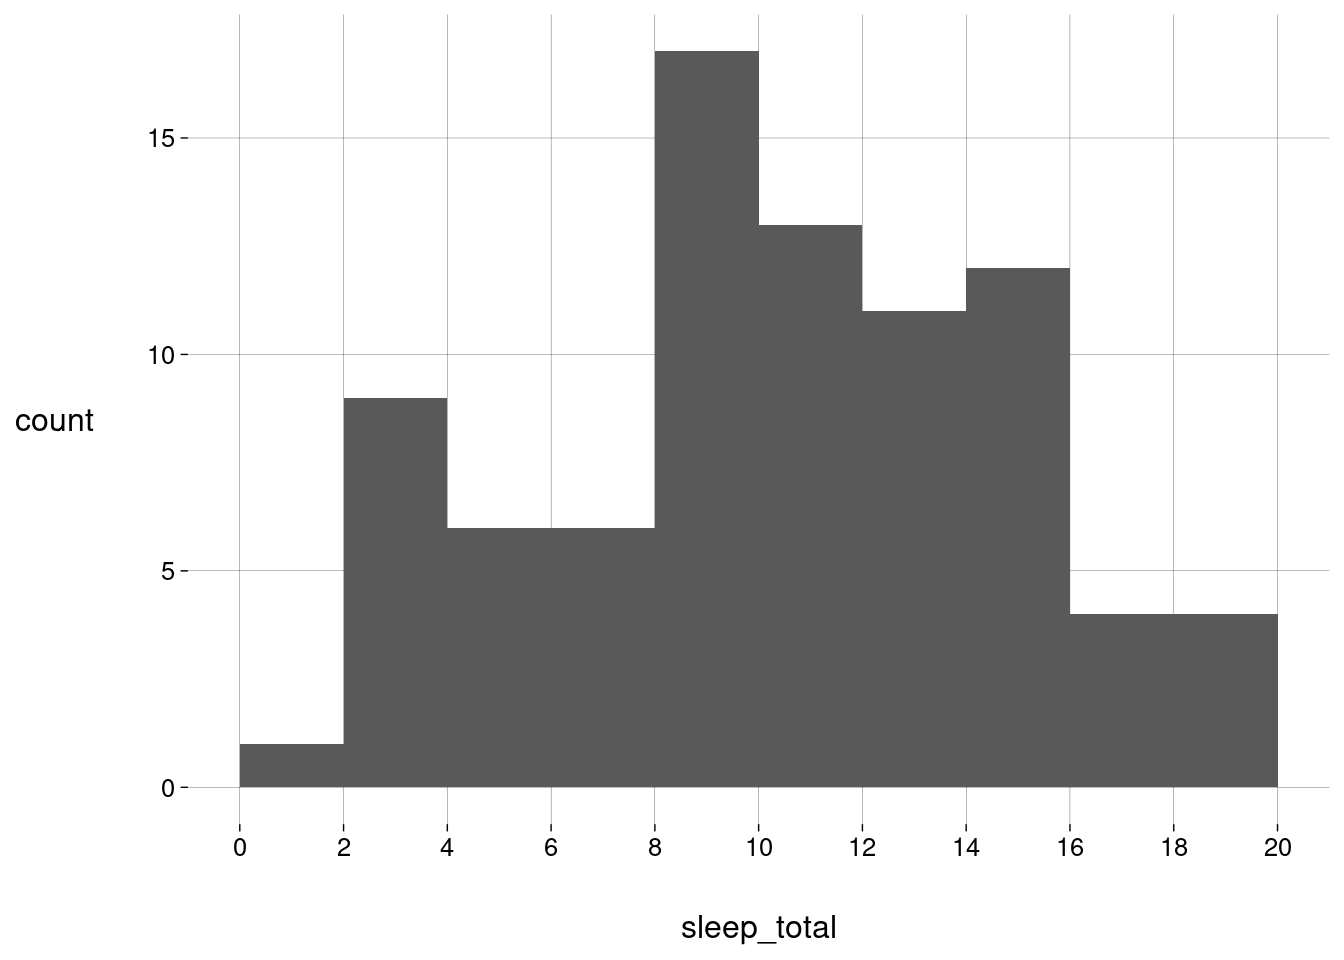
\includegraphics[width=1\linewidth]{_main_files/figure-latex/hist-sono2-1} \end{center}
\item
  Nossas impressões:

  \begin{itemize}
  \item
    A classe que mais tem elementos é a de $8$ a $10$ horas.
  \item
    A distribuição é mais ou menos simétrica.
  \item
    A distribuição tem forma aproximada de sino: há poucos mamíferos com valores extremos de horas de sono; a maioria está próxima do valor médio:

\begin{Shaded}
\begin{Highlighting}[]
\FunctionTok{mean}\NormalTok{(sono}\SpecialCharTok{$}\NormalTok{sleep\_total)}
\end{Highlighting}
\end{Shaded}

\begin{verbatim}
## [1] 10,43373
\end{verbatim}
  \end{itemize}
\end{itemize}

\hypertarget{poluxedgono-de-frequuxeancia}{%
\subsection{Polígono de frequência}\label{poluxedgono-de-frequuxeancia}}

\begin{itemize}
\item
  Em vez das barras do histograma, podemos desenhar uma linha ligando seus topos.
\item
  O resultado é um {\hl{polígono de frequência}}.

\begin{Shaded}
\begin{Highlighting}[]
\NormalTok{pf }\OtherTok{\textless{}{-}}\NormalTok{ sono }\SpecialCharTok{\%\textgreater{}\%} 
  \FunctionTok{ggplot}\NormalTok{(}\FunctionTok{aes}\NormalTok{(}\AttributeTok{x =}\NormalTok{ sleep\_total)) }\SpecialCharTok{+}
    \FunctionTok{geom\_freqpoly}\NormalTok{(}\AttributeTok{breaks =} \FunctionTok{seq}\NormalTok{(}\DecValTok{0}\NormalTok{, }\DecValTok{20}\NormalTok{, }\DecValTok{2}\NormalTok{), }\AttributeTok{color =} \StringTok{\textquotesingle{}red\textquotesingle{}}\NormalTok{) }\SpecialCharTok{+}
    \FunctionTok{scale\_x\_continuous}\NormalTok{(}\AttributeTok{breaks =} \FunctionTok{seq}\NormalTok{(}\DecValTok{0}\NormalTok{, }\DecValTok{20}\NormalTok{, }\DecValTok{2}\NormalTok{))}

\NormalTok{pf}
\end{Highlighting}
\end{Shaded}

  \begin{center}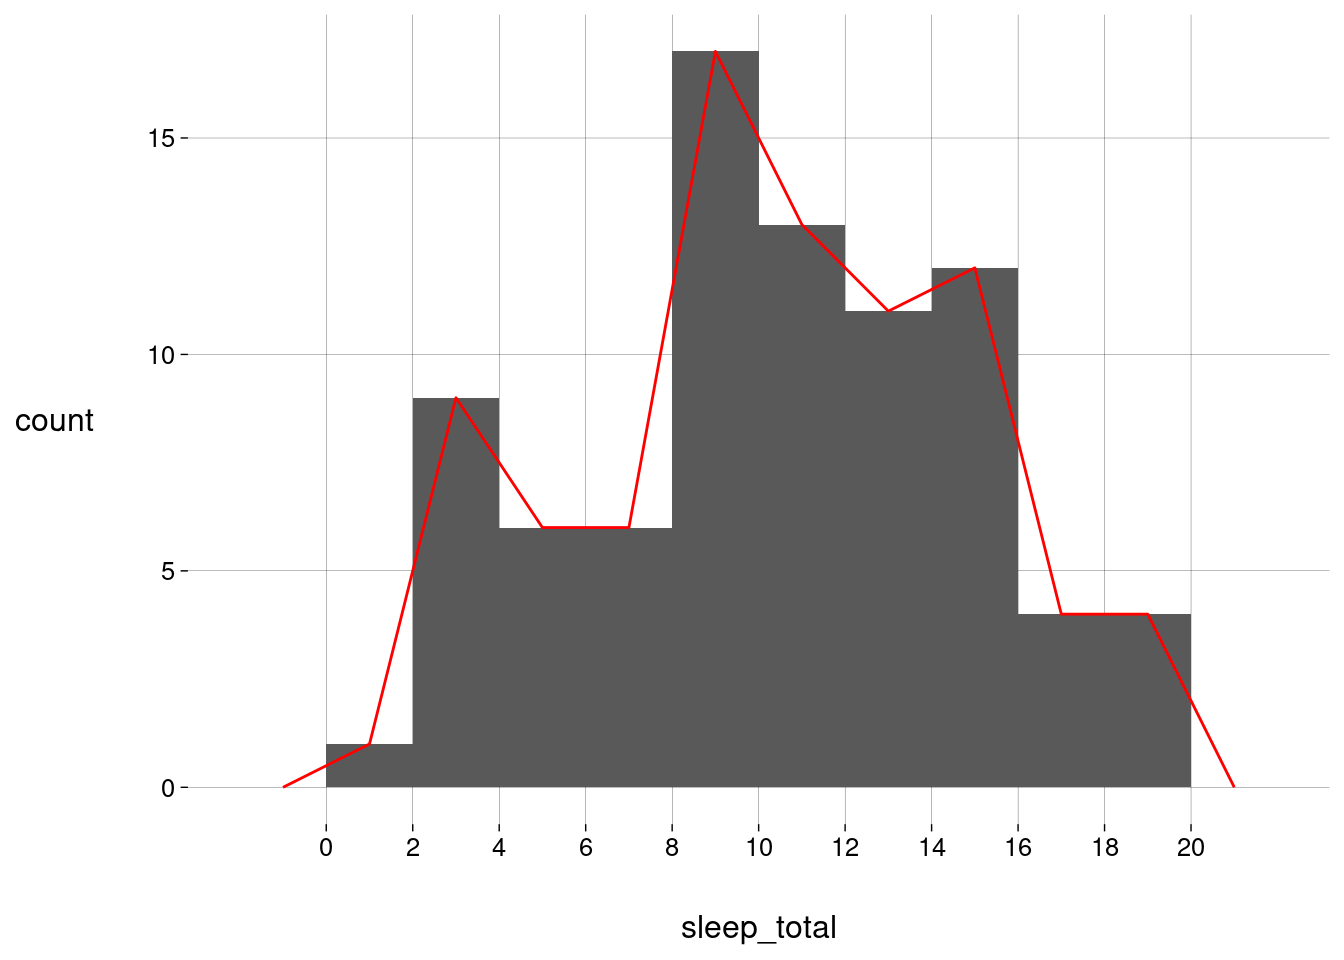
\includegraphics[width=1\linewidth]{_main_files/figure-latex/hist-freqpoly-1} \end{center}
\item
  Vamos sobrepor o polígono de frequência ao histograma, para deixar claro o que está acontecendo:

\begin{Shaded}
\begin{Highlighting}[]
\NormalTok{pf }\SpecialCharTok{+} \FunctionTok{geom\_histogram}\NormalTok{(}\AttributeTok{breaks =} \FunctionTok{seq}\NormalTok{(}\DecValTok{0}\NormalTok{, }\DecValTok{20}\NormalTok{, }\DecValTok{2}\NormalTok{), }\AttributeTok{alpha =}\NormalTok{ .}\DecValTok{3}\NormalTok{)}
\end{Highlighting}
\end{Shaded}

  \begin{center}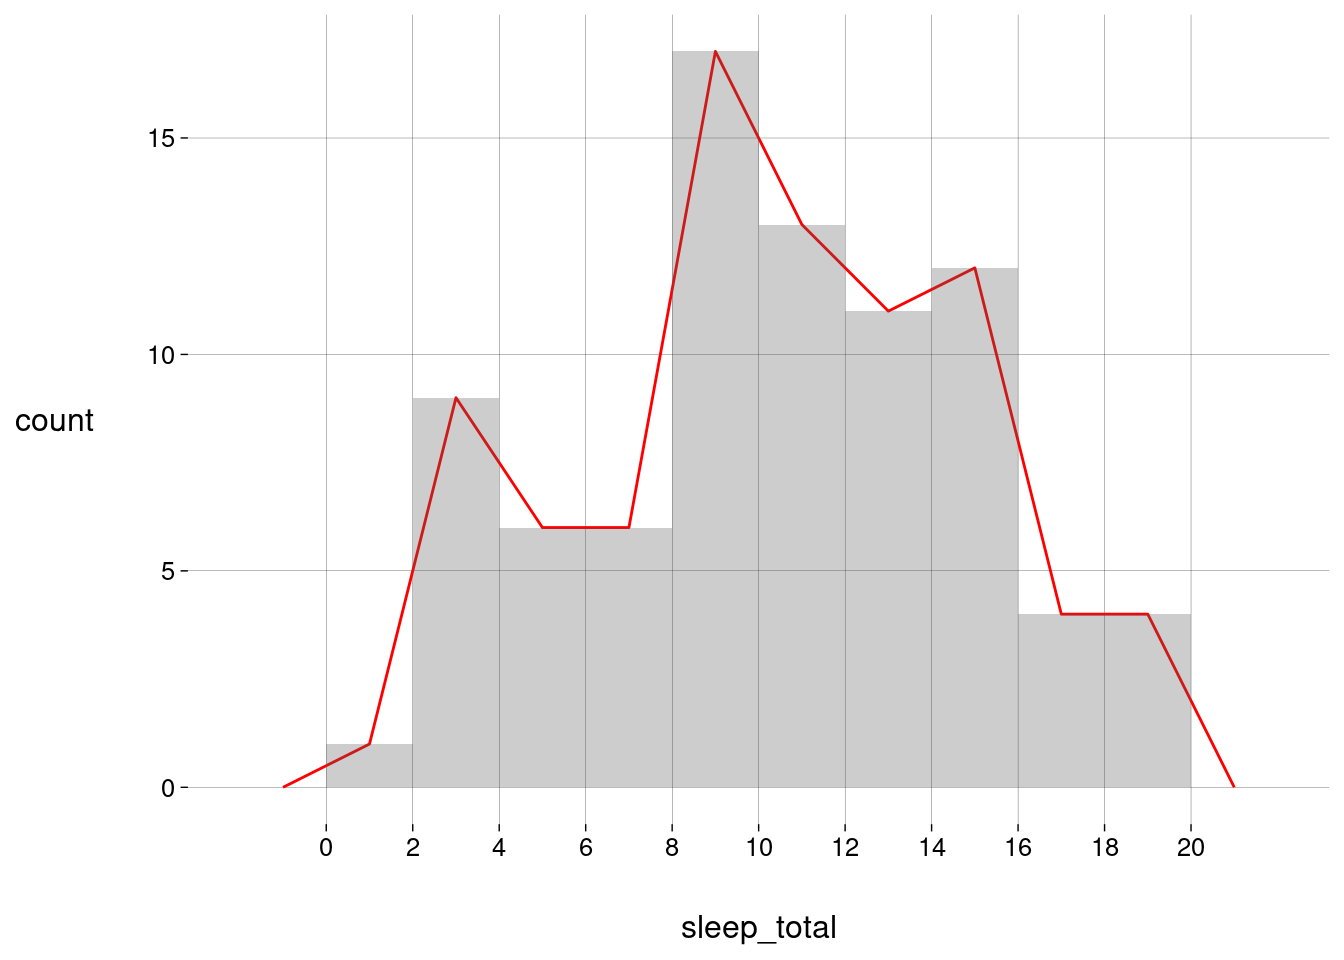
\includegraphics[width=1\linewidth]{_main_files/figure-latex/hist-freqpoly2-1} \end{center}
\end{itemize}

\hypertarget{ogiva}{%
\section{Ogiva}\label{ogiva}}

\begin{itemize}
\item
  A ogiva é um gráfico que mostra a {\hl{frequência acumulada}}: para cada valor $v$ da variável no eixo $x$, a proporção de indivíduos com valor menor ou igual a $v$.
\item
  A geometria \texttt{geom\_step} gera o gráfico de uma {\hl{função degrau}}.
\item
  Cada geometria está ligada a uma {\hl{{\mbox{\texttt{stat}}}}}, um algoritmo para computar o que vai ser desenhado. Aqui, passamos para a geometria {\hl{a função {\mbox{\texttt{ecdf}}} (\emph{empirical cumulative distribution function}), do pacote {\mbox{\texttt{stats}}}, que calcula as frequências acumuladas.}}

\begin{Shaded}
\begin{Highlighting}[]
\NormalTok{sono }\SpecialCharTok{\%\textgreater{}\%} 
  \FunctionTok{ggplot}\NormalTok{(}\FunctionTok{aes}\NormalTok{(}\AttributeTok{x =}\NormalTok{ sleep\_total)) }\SpecialCharTok{+}
    \FunctionTok{geom\_step}\NormalTok{(}\AttributeTok{stat =} \StringTok{\textquotesingle{}ecdf\textquotesingle{}}\NormalTok{) }\SpecialCharTok{+}
    \FunctionTok{scale\_x\_continuous}\NormalTok{(}\AttributeTok{breaks =} \FunctionTok{seq}\NormalTok{(}\DecValTok{0}\NormalTok{, }\DecValTok{20}\NormalTok{, }\DecValTok{2}\NormalTok{)) }\SpecialCharTok{+}
    \FunctionTok{scale\_y\_continuous}\NormalTok{(}\AttributeTok{breaks =} \FunctionTok{seq}\NormalTok{(}\DecValTok{0}\NormalTok{, }\DecValTok{1}\NormalTok{, .}\DecValTok{1}\NormalTok{)) }\SpecialCharTok{+}
    \FunctionTok{labs}\NormalTok{(}\AttributeTok{y =} \ConstantTok{NULL}\NormalTok{)}
\end{Highlighting}
\end{Shaded}

  \begin{center}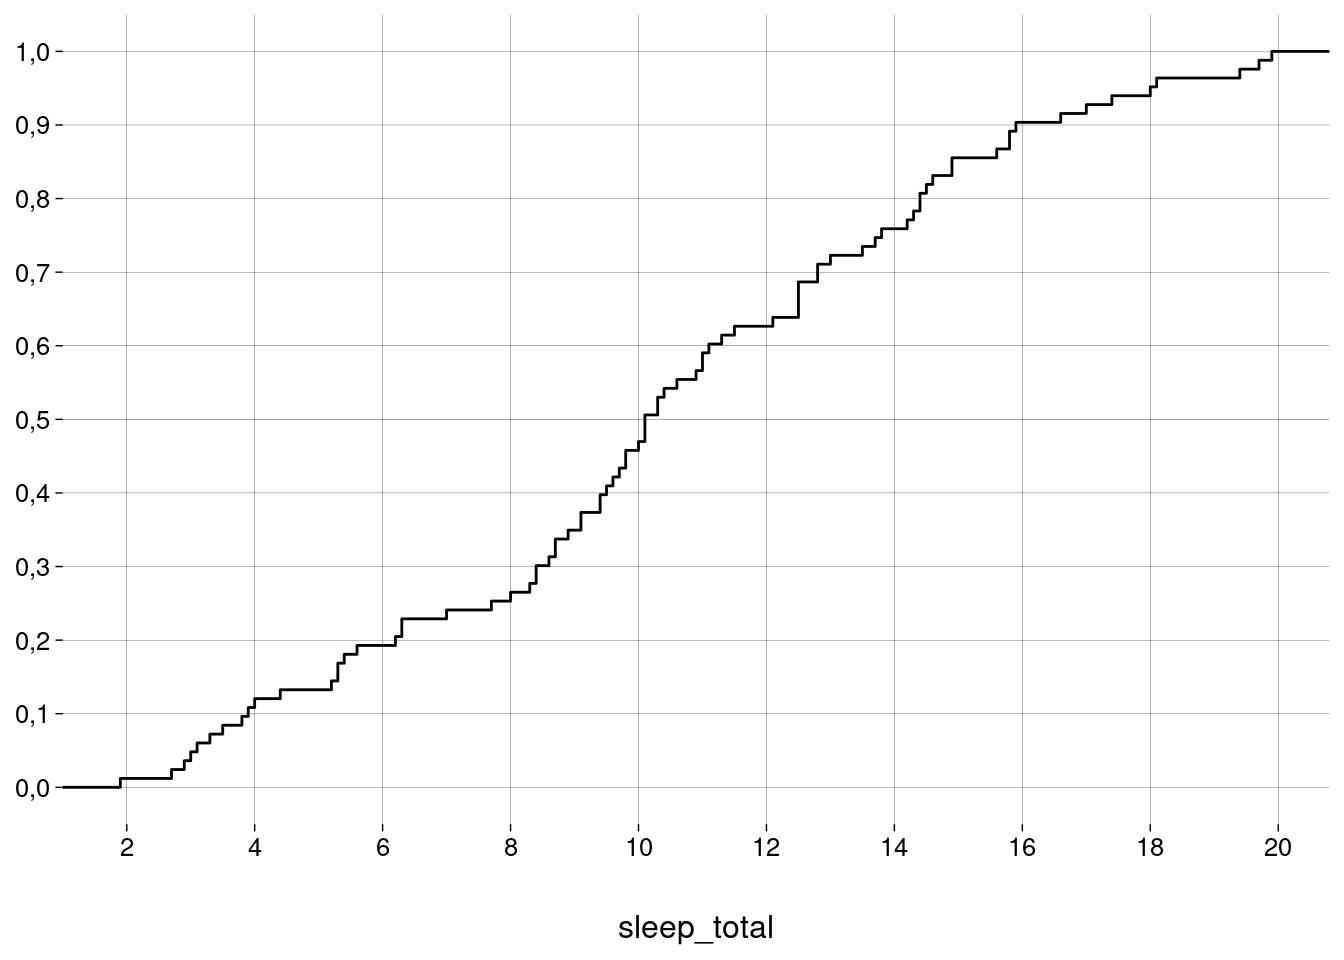
\includegraphics[width=1\linewidth]{_main_files/figure-latex/ogiva-1} \end{center}
\item
  Com a ogiva, podemos obter informações difíceis de visualizar no histograma. Por exemplo:

  \begin{itemize}
  \item
    Cerca de $20\%$ dos mamíferos têm menos de $6$ horas de sono.
  \item
    Cerca de metade dos mamíferos têm menos de $10$ horas de sono.
  \item
    Cerca de $10\%$ dos mamíferos têm mais de $16$ horas de sono.
  \end{itemize}
\end{itemize}

\hypertarget{ramos-e-folhas}{%
\section{Ramos e folhas}\label{ramos-e-folhas}}

\begin{itemize}
\item
  No início dos anos $1900$, quando estatísticas eram feitas à mão, Arthur Bowley criou os {\hl{diagramas de ramos e folhas}}.
\item
  Um diagrama de ramos e folhas é, basicamente, uma listagem de todos os valores de uma variável, agrupados de maneira que todos os valores de uma classe (i.e., de uma linha) têm os algarismos iniciais dentro de um intervalo.
\item
  Para as horas de sono dos mamíferos:

\begin{Shaded}
\begin{Highlighting}[]
\NormalTok{sono}\SpecialCharTok{$}\NormalTok{sleep\_total }\SpecialCharTok{\%\textgreater{}\%} 
  \FunctionTok{stem}\NormalTok{()}
\end{Highlighting}
\end{Shaded}

\begin{verbatim}
## 
##   The decimal point is at the |
## 
##    0 | 9
##    2 | 79013589
##    4 | 0423346
##    6 | 23307
##    8 | 03446779114456788
##   10 | 01113346900135
##   12 | 15555880578
##   14 | 234456996889
##   16 | 604
##   18 | 01479
\end{verbatim}
\item
  A primeira linha representa um indivíduo com $0{,}9$ horas de sono.
\item
  A penúltima linha representa $3$ valores:

  \begin{itemize}
  \tightlist
  \item
    $16{,}6$
  \item
    $17{,}0$
  \item
    $17{,}4$
  \end{itemize}
\end{itemize}

\hypertarget{personalizauxe7uxe3o-do-tema}{%
\section{Personalização do tema}\label{personalizauxe7uxe3o-do-tema}}

\begin{itemize}
\item
  O \texttt{ggplot2} tem um tema \emph{default}, chamado \texttt{theme\_gray}, que gera \protect\hyperlink{grafico4}{o \emph{scatterplot} de um exemplo anterior} deste capítulo do seguinte modo:

  \begin{center}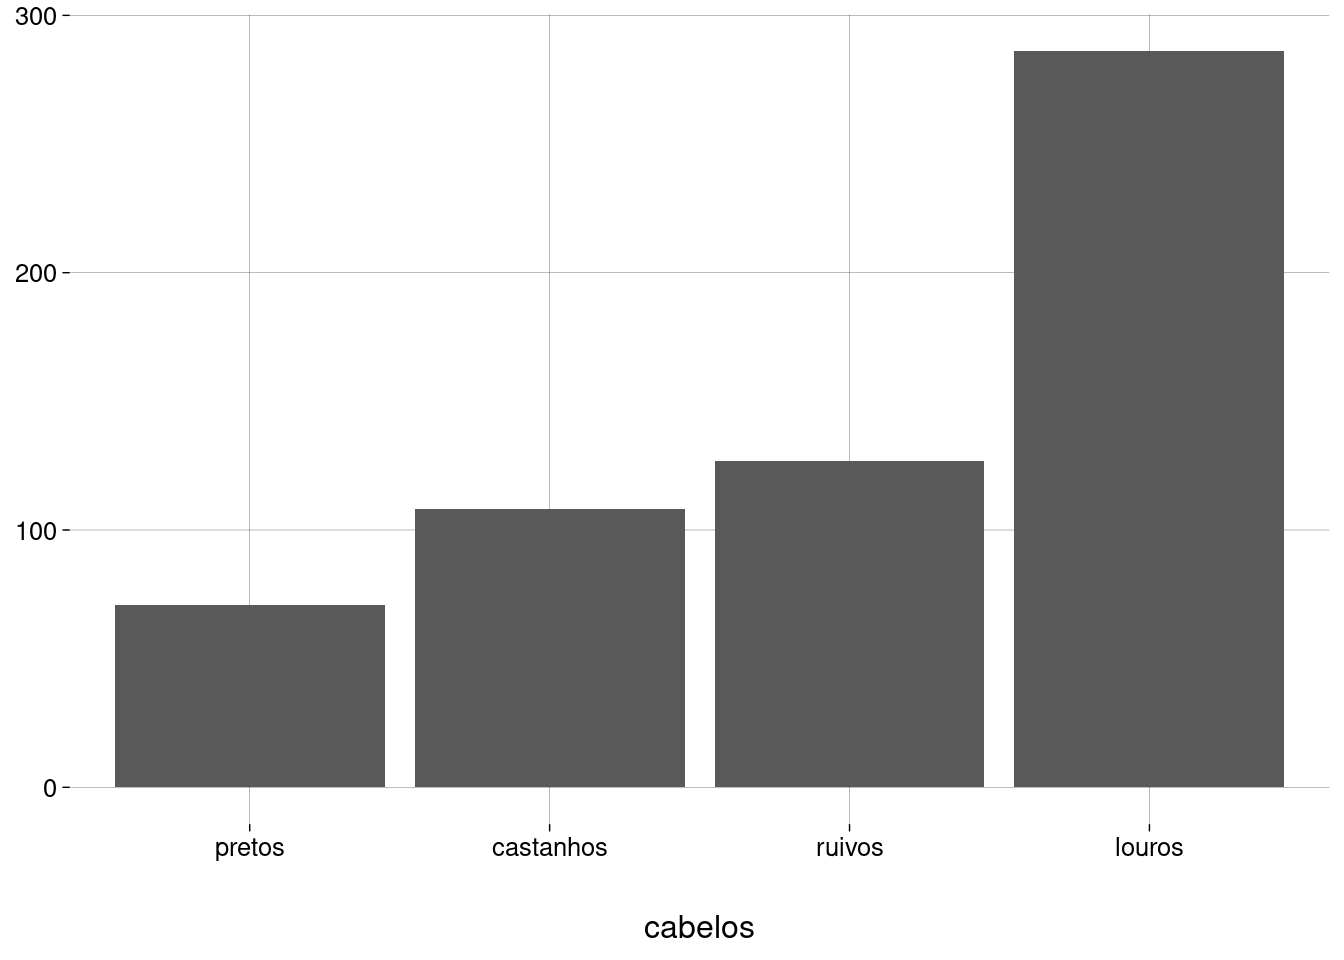
\includegraphics[width=1\linewidth]{_main_files/figure-latex/unnamed-chunk-79-1} \end{center}
\item
  Para este material, escolhi o tema \texttt{theme\_linedraw}, que usa linhas pretas sobre fundo branco:

  \begin{center}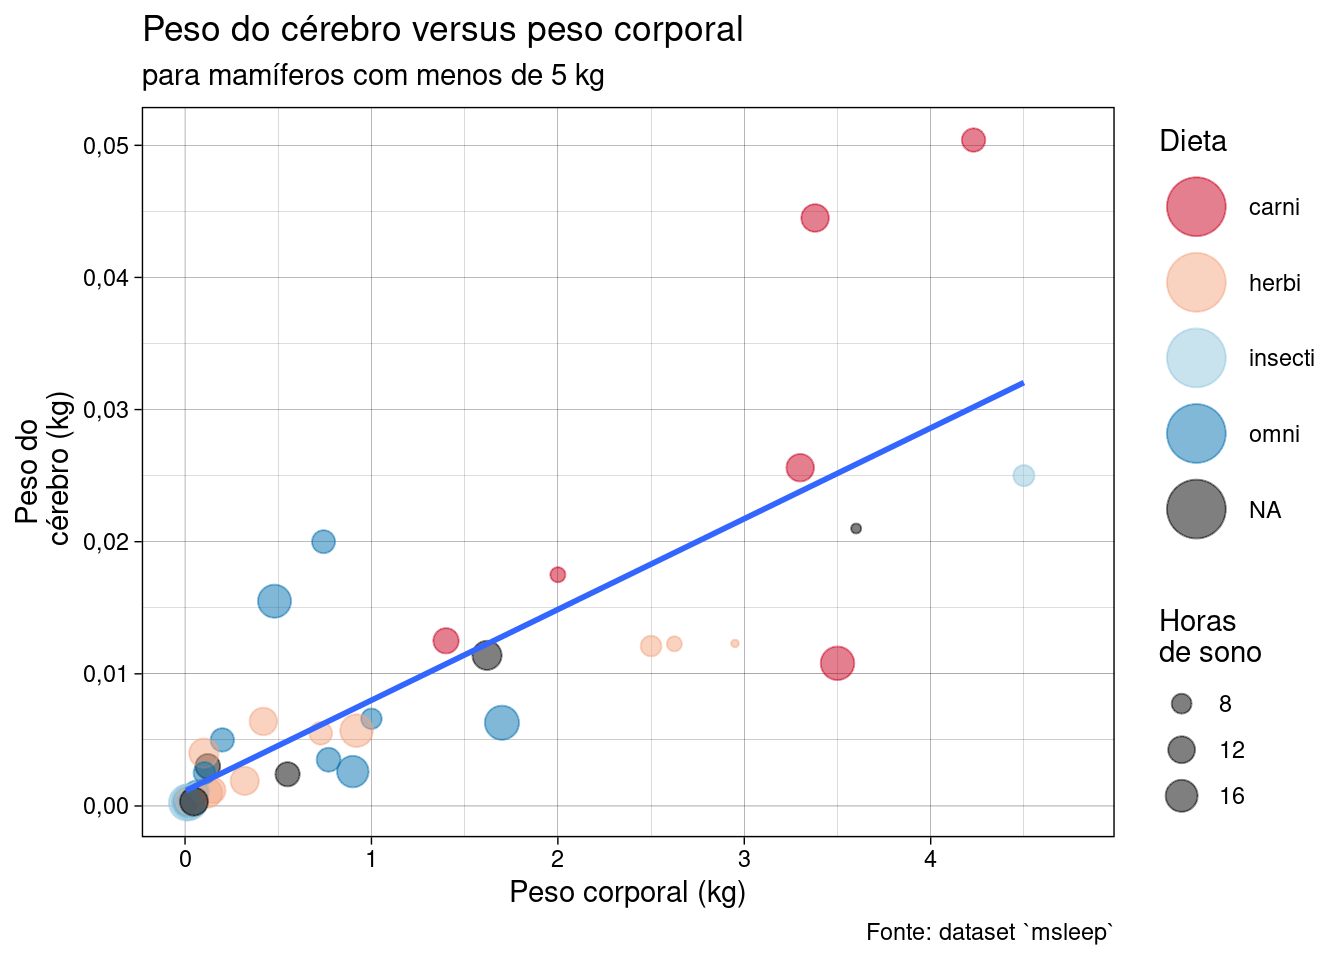
\includegraphics[width=1\linewidth]{_main_files/figure-latex/unnamed-chunk-80-1} \end{center}
\item
  Para deixar os gráficos mais leves e facilitar a leitura, fiz as seguintes alterações no tema:

  \begin{itemize}
  \item
    Mudei o tamanho do texto dos rótulos.
  \item
    Fiz o rótulo do eixo $y$ aparecer na horizontal; embora isto ocupe um pouco mais de espaço, evita que o leitor tenha que girar a cabeça para ler o rótulo.
  \item
    Eliminei as linhas dos eixos, para o gráfico ficar mais leve.
  \item
    Eliminei a moldura da área de dados, para o gráfico ficar mais leve.
  \item
    Eliminei a grade secundária, para o gráfico ficar mais leve.
  \end{itemize}
\item
  O resultado é

  \begin{center}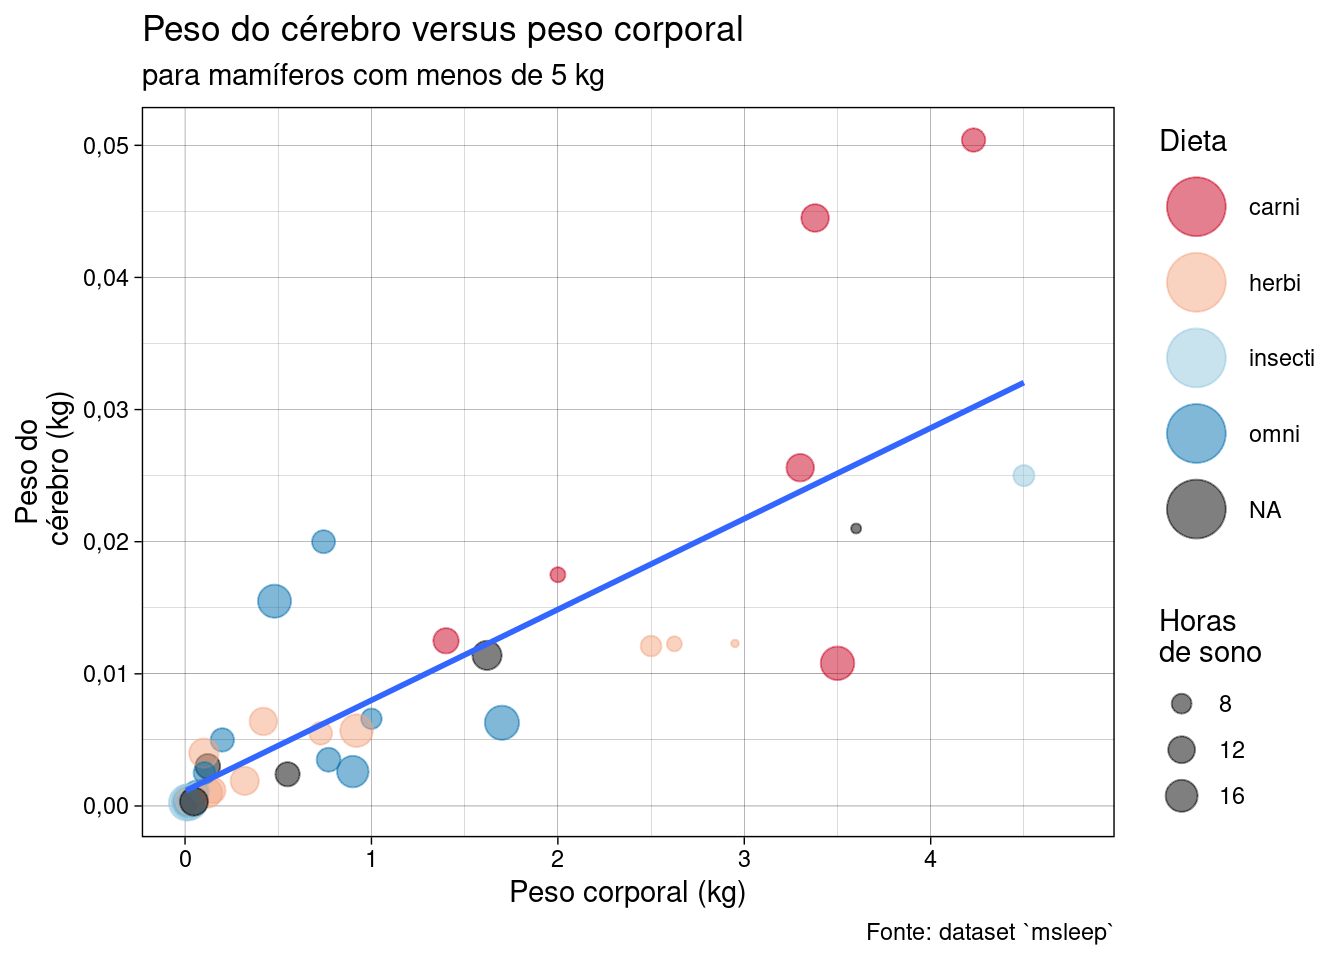
\includegraphics[width=1\linewidth]{_main_files/figure-latex/unnamed-chunk-81-1} \end{center}
\item
  Os meus comandos para alterar o tema são

\begin{Shaded}
\begin{Highlighting}[]
\CommentTok{\# Tamanho do texto depende do formato de saída (html ou pdf):}
\NormalTok{plot\_text\_size }\OtherTok{=} \FunctionTok{ifelse}\NormalTok{(}\FunctionTok{is\_html\_output}\NormalTok{(), }\DecValTok{12}\NormalTok{, }\DecValTok{13}\NormalTok{)}

\CommentTok{\# Tema mais leve:}
\FunctionTok{theme\_set}\NormalTok{(}
  \FunctionTok{theme\_linedraw}\NormalTok{() }\SpecialCharTok{+}
    \FunctionTok{theme}\NormalTok{(}
      \CommentTok{\# Tamanho do texto}
      \AttributeTok{text =} \FunctionTok{element\_text}\NormalTok{(}\AttributeTok{size =}\NormalTok{ plot\_text\_size),}
      \CommentTok{\# Eixo y}
      \AttributeTok{axis.title.y.left =} \FunctionTok{element\_text}\NormalTok{(}
        \CommentTok{\# Nunca girar o rótulo do eixo y}
        \AttributeTok{angle =} \DecValTok{0}\NormalTok{,}
        \CommentTok{\# Separar o rótulo do eixo um pouco}
        \AttributeTok{margin =} \FunctionTok{margin}\NormalTok{(}\AttributeTok{r =} \DecValTok{20}\NormalTok{),}
        \CommentTok{\# Posicionar verticalmente no meio}
        \AttributeTok{vjust =}\NormalTok{ .}\DecValTok{5}
\NormalTok{      ),}
      \CommentTok{\# Eixo y secundário (à direita), quando presente}
      \AttributeTok{axis.title.y.right =} \FunctionTok{element\_text}\NormalTok{(}
        \CommentTok{\# Nunca girar o rótulo do eixo y}
        \AttributeTok{angle =} \DecValTok{0}\NormalTok{,}
        \CommentTok{\# Separar o rótulo do eixo um pouco}
        \AttributeTok{margin =} \FunctionTok{margin}\NormalTok{(}\AttributeTok{l =} \DecValTok{20}\NormalTok{),}
        \CommentTok{\# Posicionar verticalmente no meio}
        \AttributeTok{vjust =}\NormalTok{ .}\DecValTok{5}
\NormalTok{      ),}
      \CommentTok{\# Não colocar marcas no eixo y secundário}
      \AttributeTok{axis.ticks.y.right =} \FunctionTok{element\_blank}\NormalTok{(),}
      \CommentTok{\# Separar o eixo x do rótulo um pouco mais}
      \AttributeTok{axis.title.x.bottom =} \FunctionTok{element\_text}\NormalTok{(}
        \AttributeTok{margin =} \FunctionTok{margin}\NormalTok{(}\AttributeTok{t =} \DecValTok{20}\NormalTok{)}
\NormalTok{      ),}
      \CommentTok{\# Eliminar linhas dos eixos}
      \AttributeTok{axis.line =} \FunctionTok{element\_blank}\NormalTok{(),}
      \CommentTok{\# Eliminar a moldura da área de dados}
      \AttributeTok{panel.border =} \FunctionTok{element\_blank}\NormalTok{(),}
      \CommentTok{\# Eliminar a grade secundária}
      \AttributeTok{panel.grid.minor =} \FunctionTok{element\_blank}\NormalTok{()}
\NormalTok{    )}
\NormalTok{)}
\end{Highlighting}
\end{Shaded}
\end{itemize}

\hypertarget{exercuxedcios-5}{%
\section{Exercícios}\label{exercuxedcios-5}}

\begin{rmdimportant}
Não se esqueça de incluir títulos nos gráficos e rótulos nos eixos.

\end{rmdimportant}

\hypertarget{peso-cerebral-e-peso-corporal}{%
\subsection{Peso cerebral e peso corporal}\label{peso-cerebral-e-peso-corporal}}

\begin{enumerate}
\def\labelenumi{\arabic{enumi}.}
\item
  Observe os \protect\hyperlink{grafico4}{comandos que geraram o gráfico \texttt{grafico4}}.
\item
  O que acontece se você retirar \texttt{aes(group\ =\ 1)} da chamada a \texttt{geom\_smooth}? Explique.
\item
  O que acontece se você mudar \texttt{show.legend\ =\ FALSE} para \texttt{show.legend\ =\ TRUE} na chamada a \texttt{geom\_smooth}? Explique.
\item
  O que acontece se você mudar \texttt{se\ =\ FALSE} para \texttt{se\ =\ TRUE} na chamada a \texttt{geom\_smooth}? Explique.
\item
  Acrescente ao gráfico a camada \texttt{facet\_wrap(\textasciitilde{}vore)}. O que acontece?
\item
  Examine o \emph{data frame} \texttt{sono} e identifique o único insetívoro com mais de $4$kg.
\item
  Instale o pacote \texttt{gg\_repel} e acrescente ao gráfico \texttt{grafico4} (não facetado) a geometria \texttt{geom\_label\_repel} (consulte a ajuda) para rotular o mamífero insetívoro identificado no item anterior com o seu nome, {\hl{sem cobrir outros pontos do gráfico}}. Cuidado para não alterar a legenda que já existe.
\end{enumerate}

\hypertarget{peso-cerebral-e-horas-de-sono}{%
\subsection{Peso cerebral e horas de sono}\label{peso-cerebral-e-horas-de-sono}}

\begin{rmdbox}

Use o \emph{data frame} \texttt{sono} definido como

\begin{Shaded}
\begin{Highlighting}[]
\FunctionTok{library}\NormalTok{(ggplot2)}

\NormalTok{sono }\OtherTok{\textless{}{-}}\NormalTok{ msleep }\SpecialCharTok{\%\textgreater{}\%} 
  \FunctionTok{select}\NormalTok{(}
\NormalTok{    name, order, genus, vore, bodywt, }
\NormalTok{    brainwt, awake, sleep\_total}
\NormalTok{  )}
\end{Highlighting}
\end{Shaded}

\end{rmdbox}

\begin{enumerate}
\def\labelenumi{\arabic{enumi}.}
\item
  Construa um histograma da variável \texttt{brainwt}. Escolha o número de classes que você achar melhor. O que acontece com os valores \texttt{NA}?
\item
  \href{http://sillasgonzaga.com/material/curso_visualizacao/ggplot2-parte-ii.html\#customizando-escalas}{Descubra que função da forma \texttt{scale\_x\_...} usar} para fazer com que o eixo $x$ tenha uma escala logarítmica. Gere um novo histograma.
\item
  Qual dos dois histogramas é melhor para responder a pergunta ``\emph{Qual a faixa de peso cerebral que tem mais animais?}'' de forma satisfatória?
\item
  Construa um \emph{scatter plot} de horas de sono versus peso do cérebro. Você percebe alguma correlação entre estas variáveis? Se precisar, concentre-se em um subconjunto dos dados.
\item
  Usando \texttt{geom\_smooth} (\href{https://cdr.ibpad.com.br/ggplot2.html\#objetos-geom\%C3\%A9tricos-e-tipos-de-gr\%C3\%A1ficos}{leia a respeito}), sobreponha uma reta de regressão ao gráfico de dispersão, usando o método \texttt{lm} e sem o erro padrão (i.e., com \texttt{se\ =\ FALSE}). O que você observa? Discuta.
\end{enumerate}

\hypertarget{igualdade-de-guxeanero-entre-furacuxf5es}{%
\subsection{Igualdade de gênero entre furacões?}\label{igualdade-de-guxeanero-entre-furacuxf5es}}

\href{https://www.pnas.org/content/111/24/8782}{Este artigo} tenta achar uma relação entre o gênero do nome de um furacão e a quantidade de vítimas fatais provocadas por ele.

\begin{rmdbox}

Os dados estão no pacote \texttt{DAAG}, que deve ser instalado:

\begin{Shaded}
\begin{Highlighting}[]
\ControlFlowTok{if}\NormalTok{ (}\SpecialCharTok{!}\FunctionTok{require}\NormalTok{(DAAG))}
  \FunctionTok{install.packages}\NormalTok{(}\StringTok{"DAAG"}\NormalTok{)}
\end{Highlighting}
\end{Shaded}

Vamos usar apenas algumas das variáveis, com nomes em português.

\begin{Shaded}
\begin{Highlighting}[]
\NormalTok{df }\OtherTok{\textless{}{-}}\NormalTok{ hurricNamed }\SpecialCharTok{\%\textgreater{}\%} 
  \FunctionTok{as\_tibble}\NormalTok{() }\SpecialCharTok{\%\textgreater{}\%} 
  \FunctionTok{transmute}\NormalTok{(}
    \AttributeTok{id =} \FunctionTok{paste}\NormalTok{(Year, Name, }\AttributeTok{sep =} \StringTok{\textquotesingle{}{-}\textquotesingle{}}\NormalTok{),}
    \AttributeTok{nome =}\NormalTok{ Name,}
    \AttributeTok{ano =}\NormalTok{ Year,}
    \AttributeTok{velocidade =}\NormalTok{ LF.WindsMPH }\SpecialCharTok{*} \FloatTok{1.8}\NormalTok{,     }\CommentTok{\# convertido para km/h}
    \AttributeTok{pressao =}\NormalTok{ LF.PressureMB,            }\CommentTok{\# mbar}
    \AttributeTok{prejuizo =}\NormalTok{ BaseDam2014 }\SpecialCharTok{\%\textgreater{}\%} \FunctionTok{round}\NormalTok{(), }\CommentTok{\# milhões de dólares de 2014}
    \AttributeTok{mortes =}\NormalTok{ deaths,}
    \AttributeTok{genero =}\NormalTok{ mf}
\NormalTok{  )}
\end{Highlighting}
\end{Shaded}

\end{rmdbox}

\begin{enumerate}
\def\labelenumi{\arabic{enumi}.}
\item
  Crie histogramas para as seguintes variáveis, escolhendo a quantidade de barras que você achar melhor.

  \begin{itemize}
  \item
    \texttt{velocidade}
  \item
    \texttt{prejuizo}
  \item
    \texttt{mortes}
  \end{itemize}

  Não se esqueça de incluir títulos nos gráficos e rótulos nos eixos.

  Comente os histogramas.
\item
  Os histogramas de prejuízos e mortes não ficaram bons. Vamos gerar histogramas transformados.

  No \emph{data frame}, crie duas novas colunas:

  \begin{itemize}
  \item
    \texttt{logprejuizo}: \emph{logaritmo} do prejuízo (na base $10$)
  \item
    \texttt{logmortes}: \emph{logaritmo} do número de mortes (na base $10$)
  \end{itemize}

  Agora, gere histogramas destas duas novas variáveis.
\item
  O que significa o valor do logaritmo do prejuízo na base $10$?
\item
  O que significa o valor do logaritmo do número de mortes na base $10$?
\item
  Por que o histograma do logaritmo do número de mortes vem com uma mensagem de aviso?
\item
  Por que isto não acontece com o logaritmo do prejuízo?
\item
  Faça um gráfico de dispersão com \texttt{pressao} no eixo $y$ e \texttt{velocidade} no eixo $x$.
\item
  Usando \texttt{geom\_smooth} (\href{https://cdr.ibpad.com.br/ggplot2.html\#objetos-geom\%C3\%A9tricos-e-tipos-de-gr\%C3\%A1ficos}{leia a respeito}), sobreponha uma reta de regressão ao gráfico, usando o método \texttt{lm} e sem o erro padrão (i.e., com \texttt{se\ =\ FALSE}). O que você observa? Discuta.
\item
  Faça um gráfico de dispersão com \texttt{logmortes} no eixo $y$ e \texttt{pressao} no eixo $x$.
\item
  Usando \texttt{geom\_smooth} (\href{https://cdr.ibpad.com.br/ggplot2.html\#objetos-geom\%C3\%A9tricos-e-tipos-de-gr\%C3\%A1ficos}{leia a respeito}), sobreponha uma reta de regressão ao gráfico, usando o método \texttt{lm} e sem o erro padrão (i.e., com \texttt{se\ =\ FALSE}). O que você observa? Discuta.
\item
  Faça um gráfico de dispersão com \texttt{logmortes} no eixo $y$ e \texttt{pressao} no eixo $x$, com pontos coloridos de acordo com o gênero do nome do furacão.
\item
  Usando \texttt{geom\_smooth} (\href{https://cdr.ibpad.com.br/ggplot2.html\#objetos-geom\%C3\%A9tricos-e-tipos-de-gr\%C3\%A1ficos}{leia a respeito}), sobreponha retas de regressão ao gráfico, uma para cada gênero, usando o método \texttt{lm} e sem o erro padrão (i.e., com \texttt{se\ =\ FALSE}). O que você observa? Discuta.
\end{enumerate}

\begin{rmdcaution}
Visualizações como esta ajudam a explorar os dados, mas não servem para testar rigorosamente a hipótese de que furacões mulheres matam mais do que furacões homens.

Mais adiante no curso, vamos aprender a fazer testes mais rigorosos sobre hipóteses como esta.

\end{rmdcaution}

\hypertarget{viz2}{%
\chapter{Visualização com ggplot2 (continuação)}\label{viz2}}

\begin{rmdtip}
Busque mais informações sobre os pacotes \texttt{tidyverse} e \texttt{ggplot2} \protect\hyperlink{refrec}{nas referências recomendadas}.

\end{rmdtip}

\hypertarget{vuxeddeo-1-3}{%
\section{Vídeo 1}\label{vuxeddeo-1-3}}

\begin{center} \url{https://youtu.be/TjgLDeIQHIc} \end{center}

\hypertarget{boxplots}{%
\section{\texorpdfstring{\emph{Boxplots}}{Boxplots}}\label{boxplots}}

\hypertarget{conjunto-de-dados}{%
\subsection{Conjunto de dados}\label{conjunto-de-dados}}

\begin{itemize}
\item
  Vamos continuar a trabalhar com os dados sobre as horas de sono de alguns mamíferos:

\begin{Shaded}
\begin{Highlighting}[]
\NormalTok{sono }\OtherTok{\textless{}{-}}\NormalTok{ msleep }\SpecialCharTok{\%\textgreater{}\%} 
  \FunctionTok{select}\NormalTok{(name, vore, order, sleep\_total)}

\NormalTok{sono}
\end{Highlighting}
\end{Shaded}

\begin{verbatim}
## # A tibble: 83 x 4
##   name                       vore  order        sleep_total
##   <chr>                      <chr> <chr>              <dbl>
## 1 Cheetah                    carni Carnivora           12.1
## 2 Owl monkey                 omni  Primates            17  
## 3 Mountain beaver            herbi Rodentia            14.4
## 4 Greater short-tailed shrew omni  Soricomorpha        14.9
## 5 Cow                        herbi Artiodactyla         4  
## 6 Three-toed sloth           herbi Pilosa              14.4
## # ... with 77 more rows
\end{verbatim}
\end{itemize}

\hypertarget{mediana}{%
\subsection{Mediana e quartis}\label{mediana}}

\begin{itemize}
\item
  Para entender \emph{boxplots}, precisamos, antes, entender algumas medidas.
\item
  Se tomarmos as quantidades de horas de sono de todos os animais do conjunto de dados e {\hl{classificarmos estas quantidades em ordem crescente}}, vamos ter:

\begin{Shaded}
\begin{Highlighting}[]
\NormalTok{horas }\OtherTok{\textless{}{-}}\NormalTok{ sono }\SpecialCharTok{\%\textgreater{}\%} 
  \FunctionTok{pull}\NormalTok{(sleep\_total) }\SpecialCharTok{\%\textgreater{}\%} 
  \FunctionTok{sort}\NormalTok{()}

\NormalTok{horas}
\end{Highlighting}
\end{Shaded}

\begin{verbatim}
##  [1]  1,9  2,7  2,9  3,0  3,1  3,3  3,5  3,8  3,9  4,0  4,4  5,2  5,3
## [14]  5,3  5,4  5,6  6,2  6,3  6,3  7,0  7,7  8,0  8,3  8,4  8,4  8,6
## [27]  8,7  8,7  8,9  9,1  9,1  9,4  9,4  9,5  9,6  9,7  9,8  9,8 10,0
## [40] 10,1 10,1 10,1 10,3 10,3 10,4 10,6 10,9 11,0 11,0 11,1 11,3 11,5
## [53] 12,1 12,5 12,5 12,5 12,5 12,8 12,8 13,0 13,5 13,7 13,8 14,2 14,3
## [66] 14,4 14,4 14,5 14,6 14,9 14,9 15,6 15,8 15,8 15,9 16,6 17,0 17,4
## [79] 18,0 18,1 19,4 19,7 19,9
\end{verbatim}
\item
  Quantos valores são?

\begin{Shaded}
\begin{Highlighting}[]
\FunctionTok{length}\NormalTok{(horas)}
\end{Highlighting}
\end{Shaded}

\begin{verbatim}
## [1] 83
\end{verbatim}
\item
  O valor que está {\hl{bem no meio desta fila}} --- i.e., na posição $42$ --- é a {\hl{mediana}}:

\begin{Shaded}
\begin{Highlighting}[]
\NormalTok{horas[}\FunctionTok{ceiling}\NormalTok{(}\FunctionTok{length}\NormalTok{(horas) }\SpecialCharTok{/} \DecValTok{2}\NormalTok{)]}
\end{Highlighting}
\end{Shaded}

\begin{verbatim}
## [1] 10,1
\end{verbatim}
\item
  Em R:

\begin{Shaded}
\begin{Highlighting}[]
\FunctionTok{median}\NormalTok{(horas)}
\end{Highlighting}
\end{Shaded}

\begin{verbatim}
## [1] 10,1
\end{verbatim}

  \begin{rmdcaution}
  Mediana e média são coisas muito diferentes.

  Por acaso, neste exemplo, a média das horas é próxima da mediana:

\begin{Shaded}
\begin{Highlighting}[]
\FunctionTok{mean}\NormalTok{(horas)}
\end{Highlighting}
\end{Shaded}

\begin{verbatim}
## [1] 10,43373
\end{verbatim}

  Isto costuma acontecer quando a distribuição dos dados é aproximadamente simétrica.

  \end{rmdcaution}
\item
  Os {\hl{quartis}} são os valores que estão nas posições $\frac14$, $\frac12$ e $\frac34$ da fila. São o {\hl{primeiro, segundo e terceiro quartis}}, respectivamente.

\begin{Shaded}
\begin{Highlighting}[]
\NormalTok{horas[}
  \FunctionTok{c}\NormalTok{(}
    \FunctionTok{ceiling}\NormalTok{(}\FunctionTok{length}\NormalTok{(horas) }\SpecialCharTok{/} \DecValTok{4}\NormalTok{),}
    \FunctionTok{ceiling}\NormalTok{(}\FunctionTok{length}\NormalTok{(horas) }\SpecialCharTok{/} \DecValTok{2}\NormalTok{),}
    \FunctionTok{ceiling}\NormalTok{(}\DecValTok{3} \SpecialCharTok{*} \FunctionTok{length}\NormalTok{(horas) }\SpecialCharTok{/} \DecValTok{4}\NormalTok{)}
\NormalTok{  )}
\NormalTok{]}
\end{Highlighting}
\end{Shaded}

\begin{verbatim}
## [1]  7,7 10,1 13,8
\end{verbatim}
\item
  {\hl{Sim, a mediana é o segundo quartil.}}
\item
  Em R, a {\hl{função {\mbox{\texttt{quantile}}}}} generaliza esta idéia: dado um número $q$ entre $0$ e $1$, {\hl{o quantil (com ``N'') $q$ é o elemento que está na posição que corresponde à fração $q$ da fila ordenada.}}

\begin{Shaded}
\begin{Highlighting}[]
\NormalTok{horas }\SpecialCharTok{\%\textgreater{}\%} \FunctionTok{quantile}\NormalTok{(}\FunctionTok{c}\NormalTok{(.}\DecValTok{25}\NormalTok{, .}\DecValTok{5}\NormalTok{, .}\DecValTok{75}\NormalTok{))}
\end{Highlighting}
\end{Shaded}

\begin{verbatim}
##   25%   50%   75% 
##  7,85 10,10 13,75
\end{verbatim}
\item
  Na verdade, R tem $9$ algoritmos diferentes para calcular os quantis de uma amostra! Leia a ajuda da função \texttt{quantile} para conhecê-los.
\item
  As diferenças entre nossos cálculos ``à mão'' e os resultados retornados por \texttt{quantile} são porque, em algumas situações, \texttt{quantile} calcula uma média ponderada entre elementos vizinhos. Por isso, \texttt{quantile} pode retornar valores que nem estão no vetor.
\item
  Em R, a {\hl{função {\mbox{\texttt{summary}}}}} mostra o {\hl{mínimo}}, os {\hl{quartis (com ``R'')}}, a {\hl{média}}, e o {\hl{máximo}} de um vetor:

\begin{Shaded}
\begin{Highlighting}[]
\FunctionTok{summary}\NormalTok{(horas)}
\end{Highlighting}
\end{Shaded}

\begin{verbatim}
##    Min. 1st Qu.  Median    Mean 3rd Qu.    Max. 
##    1,90    7,85   10,10   10,43   13,75   19,90
\end{verbatim}
\end{itemize}

\hypertarget{muxe9dia-times-mediana}{%
\subsection{\texorpdfstring{Média $\times$ mediana}{Média  mediana}}\label{muxe9dia-times-mediana}}

\begin{itemize}
\item
  Vamos ver um exemplo simples para entender a diferença entre a média e a mediana.
\item
  Imagine o seguinte vetor com as receitas mensais de algumas pessoas (em milhares de reais:)

\begin{Shaded}
\begin{Highlighting}[]
\NormalTok{receitas }\OtherTok{\textless{}{-}} \FunctionTok{c}\NormalTok{(}\DecValTok{1}\NormalTok{, }\DecValTok{2}\NormalTok{, }\DecValTok{2}\NormalTok{, }\FloatTok{3.5}\NormalTok{, }\DecValTok{1}\NormalTok{, }\DecValTok{4}\NormalTok{, }\DecValTok{1}\NormalTok{)}
\end{Highlighting}
\end{Shaded}
\item
  Eis a mediana e a média deste vetor:

\begin{Shaded}
\begin{Highlighting}[]
\FunctionTok{summary}\NormalTok{(receitas)[}\FunctionTok{c}\NormalTok{(}\StringTok{\textquotesingle{}Median\textquotesingle{}}\NormalTok{, }\StringTok{\textquotesingle{}Mean\textquotesingle{}}\NormalTok{)]}
\end{Highlighting}
\end{Shaded}

\begin{verbatim}
##   Median     Mean 
## 2,000000 2,071429
\end{verbatim}
\item
  A mediana e a média são bem próximas.
\item
  Imagine, agora, que adicionamos ao vetor um sujeito com receita mensal de $100$ mil reais:

\begin{Shaded}
\begin{Highlighting}[]
\NormalTok{receitas }\OtherTok{\textless{}{-}} \FunctionTok{c}\NormalTok{(}\DecValTok{1}\NormalTok{, }\DecValTok{2}\NormalTok{, }\DecValTok{2}\NormalTok{, }\FloatTok{3.5}\NormalTok{, }\DecValTok{1}\NormalTok{, }\DecValTok{4}\NormalTok{, }\DecValTok{1}\NormalTok{, }\DecValTok{100}\NormalTok{)}
\end{Highlighting}
\end{Shaded}
\item
  Eis a nova mediana e a nova média:

\begin{Shaded}
\begin{Highlighting}[]
\FunctionTok{summary}\NormalTok{(receitas)[}\FunctionTok{c}\NormalTok{(}\StringTok{\textquotesingle{}Median\textquotesingle{}}\NormalTok{, }\StringTok{\textquotesingle{}Mean\textquotesingle{}}\NormalTok{)]}
\end{Highlighting}
\end{Shaded}

\begin{verbatim}
##  Median    Mean 
##  2,0000 14,3125
\end{verbatim}
\item
  O sujeito com a receita de $2$ mil reais continua no meio da fila, mas a média (que é a soma de todas as receitas, dividida pelo número de indivíduos) ficou muito diferente.
\item
  A receita do novo sujeito é um {\hl{valor discrepante}}, ou, em inglês, um {\hl{\emph{outlier}}}.
\end{itemize}

\begin{rmdimportant}
\textbf{Conclusão:}

A {\hl{mediana é robusta}}, pouco afetada por \emph{outliers}.

A {\hl{média é pouco robusta}}, muito sensível a \emph{outliers}.

\end{rmdimportant}

\hypertarget{intervalo-interquartil-iqr-e-outliers}{%
\subsection{\texorpdfstring{Intervalo interquartil (IQR) e \emph{outliers}}{Intervalo interquartil (IQR) e outliers}}\label{intervalo-interquartil-iqr-e-outliers}}

\begin{itemize}
\item
  Qual fração dos elementos está {\hl{entre o primeiro e o terceiro quartis?}}

\begin{Shaded}
\begin{Highlighting}[]
\FunctionTok{length}\NormalTok{(}
\NormalTok{  horas[}\FunctionTok{between}\NormalTok{(horas, }\FunctionTok{quantile}\NormalTok{(horas, .}\DecValTok{25}\NormalTok{), }\FunctionTok{quantile}\NormalTok{(horas, .}\DecValTok{75}\NormalTok{))]}
\NormalTok{) }\SpecialCharTok{/}
\FunctionTok{length}\NormalTok{(}
\NormalTok{  horas}
\NormalTok{)}
\end{Highlighting}
\end{Shaded}

\begin{verbatim}
## [1] 0,4939759
\end{verbatim}
\item
  {\hl{Metade}} do total de elementos está entre o primeiro e o terceiro quartis.
\item
  Este é o chamado {\hl{intervalo interquartil}} (\emph{interquartile range}, em inglês).
\item
  No nosso vetor \texttt{horas}, os {\hl{limites do IQR}} são

\begin{Shaded}
\begin{Highlighting}[]
\FunctionTok{quantile}\NormalTok{(horas, }\FunctionTok{c}\NormalTok{(.}\DecValTok{25}\NormalTok{, .}\DecValTok{75}\NormalTok{))}
\end{Highlighting}
\end{Shaded}

\begin{verbatim}
##   25%   75% 
##  7,85 13,75
\end{verbatim}
\item
  O {\hl{comprimento}} deste intervalo é calculado pela função \texttt{IQR}:

\begin{Shaded}
\begin{Highlighting}[]
\FunctionTok{IQR}\NormalTok{(horas)}
\end{Highlighting}
\end{Shaded}

\begin{verbatim}
## [1] 5,9
\end{verbatim}
\item
  Valores {\hl{muito abaixo do primeiro quartil}} podem ser considerados discrepantes (\emph{outliers}), mas quão abaixo?
\item
  A resposta (puramente convencional) é {\hl{$1{,}5 \times \text{IQR}$ abaixo do primeiro quartil.}}
\item
  No nosso vetor \texttt{horas}, isto significa valores abaixo de

\begin{Shaded}
\begin{Highlighting}[]
\NormalTok{limite\_inferior }\OtherTok{\textless{}{-}} \FunctionTok{quantile}\NormalTok{(horas, .}\DecValTok{25}\NormalTok{) }\SpecialCharTok{{-}} \FloatTok{1.5} \SpecialCharTok{*} \FunctionTok{IQR}\NormalTok{(horas)}

\FunctionTok{unname}\NormalTok{(limite\_inferior)}
\end{Highlighting}
\end{Shaded}

\begin{verbatim}
## [1] -1
\end{verbatim}
\item
  Neste caso, não há \emph{outliers}:

\begin{Shaded}
\begin{Highlighting}[]
\NormalTok{horas[horas }\SpecialCharTok{\textless{}}\NormalTok{ limite\_inferior]}
\end{Highlighting}
\end{Shaded}

\begin{verbatim}
## numeric(0)
\end{verbatim}
\item
  Da mesma forma, valores {\hl{muito acima do terceiro quartil}} podem ser considerados discrepantes (\emph{outliers}), mas quão acima?
\item
  De novo, a resposta (puramente convencional) é {\hl{$1{,}5 \times \text{IQR}$ acima do terceiro quartil.}}
\item
  No nosso vetor \texttt{horas}, isto significa valores acima de

\begin{Shaded}
\begin{Highlighting}[]
\NormalTok{limite\_superior }\OtherTok{\textless{}{-}} \FunctionTok{quantile}\NormalTok{(horas, .}\DecValTok{75}\NormalTok{) }\SpecialCharTok{+} \FloatTok{1.5} \SpecialCharTok{*} \FunctionTok{IQR}\NormalTok{(horas)}

\FunctionTok{unname}\NormalTok{(limite\_superior)}
\end{Highlighting}
\end{Shaded}

\begin{verbatim}
## [1] 22,6
\end{verbatim}
\item
  Neste caso, também não há \emph{outliers}:

\begin{Shaded}
\begin{Highlighting}[]
\NormalTok{horas[horas }\SpecialCharTok{\textgreater{}}\NormalTok{ limite\_superior]}
\end{Highlighting}
\end{Shaded}

\begin{verbatim}
## numeric(0)
\end{verbatim}
\item
  Outro exemplo: vamos tomar apenas os mamíferos onívoros:

\begin{Shaded}
\begin{Highlighting}[]
\NormalTok{onivoros }\OtherTok{\textless{}{-}}\NormalTok{ sono }\SpecialCharTok{\%\textgreater{}\%} 
  \FunctionTok{filter}\NormalTok{(vore }\SpecialCharTok{==} \StringTok{\textquotesingle{}omni\textquotesingle{}}\NormalTok{)}

\NormalTok{onivoros}
\end{Highlighting}
\end{Shaded}

\begin{verbatim}
## # A tibble: 20 x 4
##   name                       vore  order        sleep_total
##   <chr>                      <chr> <chr>              <dbl>
## 1 Owl monkey                 omni  Primates            17  
## 2 Greater short-tailed shrew omni  Soricomorpha        14.9
## 3 Grivet                     omni  Primates            10  
## 4 Star-nosed mole            omni  Soricomorpha        10.3
## 5 African giant pouched rat  omni  Rodentia             8.3
## 6 Lesser short-tailed shrew  omni  Soricomorpha         9.1
## # ... with 14 more rows
\end{verbatim}
\item
  Vamos extrair o vetor de horas de sono:

\begin{Shaded}
\begin{Highlighting}[]
\NormalTok{horas }\OtherTok{\textless{}{-}}\NormalTok{ onivoros }\SpecialCharTok{\%\textgreater{}\%} 
  \FunctionTok{pull}\NormalTok{(sleep\_total)}

\NormalTok{horas}
\end{Highlighting}
\end{Shaded}

\begin{verbatim}
##  [1] 17,0 14,9 10,0 10,3  8,3  9,1 18,0 10,1 10,9  9,8  8,0 10,1  9,7
## [14]  9,4 11,0  8,7  9,6  9,1 15,6  8,9
\end{verbatim}
\item
  Vamos calcular o primeiro e terceiro quartis:

\begin{Shaded}
\begin{Highlighting}[]
\NormalTok{quartis }\OtherTok{\textless{}{-}}\NormalTok{ horas }\SpecialCharTok{\%\textgreater{}\%} 
  \FunctionTok{quantile}\NormalTok{(}\FunctionTok{c}\NormalTok{(.}\DecValTok{25}\NormalTok{, .}\DecValTok{75}\NormalTok{))}

\NormalTok{quartis}
\end{Highlighting}
\end{Shaded}

\begin{verbatim}
##    25%    75% 
##  9,100 10,925
\end{verbatim}
\item
  Vamos achar o IQR:

\begin{Shaded}
\begin{Highlighting}[]
\FunctionTok{IQR}\NormalTok{(horas)}
\end{Highlighting}
\end{Shaded}

\begin{verbatim}
## [1] 1,825
\end{verbatim}
\item
  E os limites a partir dos quais os valores são \emph{outliers}:

\begin{Shaded}
\begin{Highlighting}[]
\NormalTok{limites }\OtherTok{\textless{}{-}}\NormalTok{ quartis }\SpecialCharTok{+} \FunctionTok{c}\NormalTok{(}\SpecialCharTok{{-}}\DecValTok{1}\NormalTok{, }\DecValTok{1}\NormalTok{) }\SpecialCharTok{*} \FloatTok{1.5} \SpecialCharTok{*} \FunctionTok{IQR}\NormalTok{(horas)}

\FunctionTok{unname}\NormalTok{(limites)}
\end{Highlighting}
\end{Shaded}

\begin{verbatim}
## [1]  6,3625 13,6625
\end{verbatim}
\item
  Existem \emph{outliers} inferiores?

\begin{Shaded}
\begin{Highlighting}[]
\NormalTok{onivoros }\SpecialCharTok{\%\textgreater{}\%} 
  \FunctionTok{filter}\NormalTok{(sleep\_total }\SpecialCharTok{\textless{}}\NormalTok{ limites[}\DecValTok{1}\NormalTok{])}
\end{Highlighting}
\end{Shaded}

\begin{verbatim}
## # A tibble: 0 x 4
## # ... with 4 variables: name <chr>, vore <chr>, order <chr>,
## #   sleep_total <dbl>
\end{verbatim}

  Não.
\item
  Existem \emph{outliers} superiores?

\begin{Shaded}
\begin{Highlighting}[]
\NormalTok{onivoros }\SpecialCharTok{\%\textgreater{}\%} 
  \FunctionTok{filter}\NormalTok{(sleep\_total }\SpecialCharTok{\textgreater{}}\NormalTok{ limites[}\DecValTok{2}\NormalTok{])}
\end{Highlighting}
\end{Shaded}

\begin{verbatim}
## # A tibble: 4 x 4
##   name                       vore  order           sleep_total
##   <chr>                      <chr> <chr>                 <dbl>
## 1 Owl monkey                 omni  Primates               17  
## 2 Greater short-tailed shrew omni  Soricomorpha           14.9
## 3 North American Opossum     omni  Didelphimorphia        18  
## 4 Tenrec                     omni  Afrosoricida           15.6
\end{verbatim}

  Sim! Estes animais dormem demais em comparação com os outros onívoros.
\end{itemize}

\hypertarget{gerando-boxplots}{%
\subsection{Gerando boxplots}\label{gerando-boxplots}}

\begin{itemize}
\item
  {\hl{Um \emph{boxplot} é uma representação visual dos valores que calculamos acima.}}
\item
  No \texttt{ggplot2}, {\hl{a geometria {\mbox{\texttt{geom\_boxplot}}} constrói \emph{boxplots}:}}

\begin{Shaded}
\begin{Highlighting}[]
\NormalTok{sono }\SpecialCharTok{\%\textgreater{}\%} 
  \FunctionTok{ggplot}\NormalTok{(}\FunctionTok{aes}\NormalTok{(}\AttributeTok{y =}\NormalTok{ sleep\_total)) }\SpecialCharTok{+}
    \FunctionTok{geom\_boxplot}\NormalTok{(}\AttributeTok{fill =} \StringTok{\textquotesingle{}gray\textquotesingle{}}\NormalTok{) }\SpecialCharTok{+}
    \FunctionTok{scale\_x\_continuous}\NormalTok{(}\AttributeTok{breaks =} \ConstantTok{NULL}\NormalTok{) }\SpecialCharTok{+}
    \FunctionTok{scale\_y\_continuous}\NormalTok{(}\AttributeTok{breaks =} \FunctionTok{seq}\NormalTok{(}\DecValTok{0}\NormalTok{, }\DecValTok{20}\NormalTok{, }\DecValTok{2}\NormalTok{))}
\end{Highlighting}
\end{Shaded}

  \begin{center}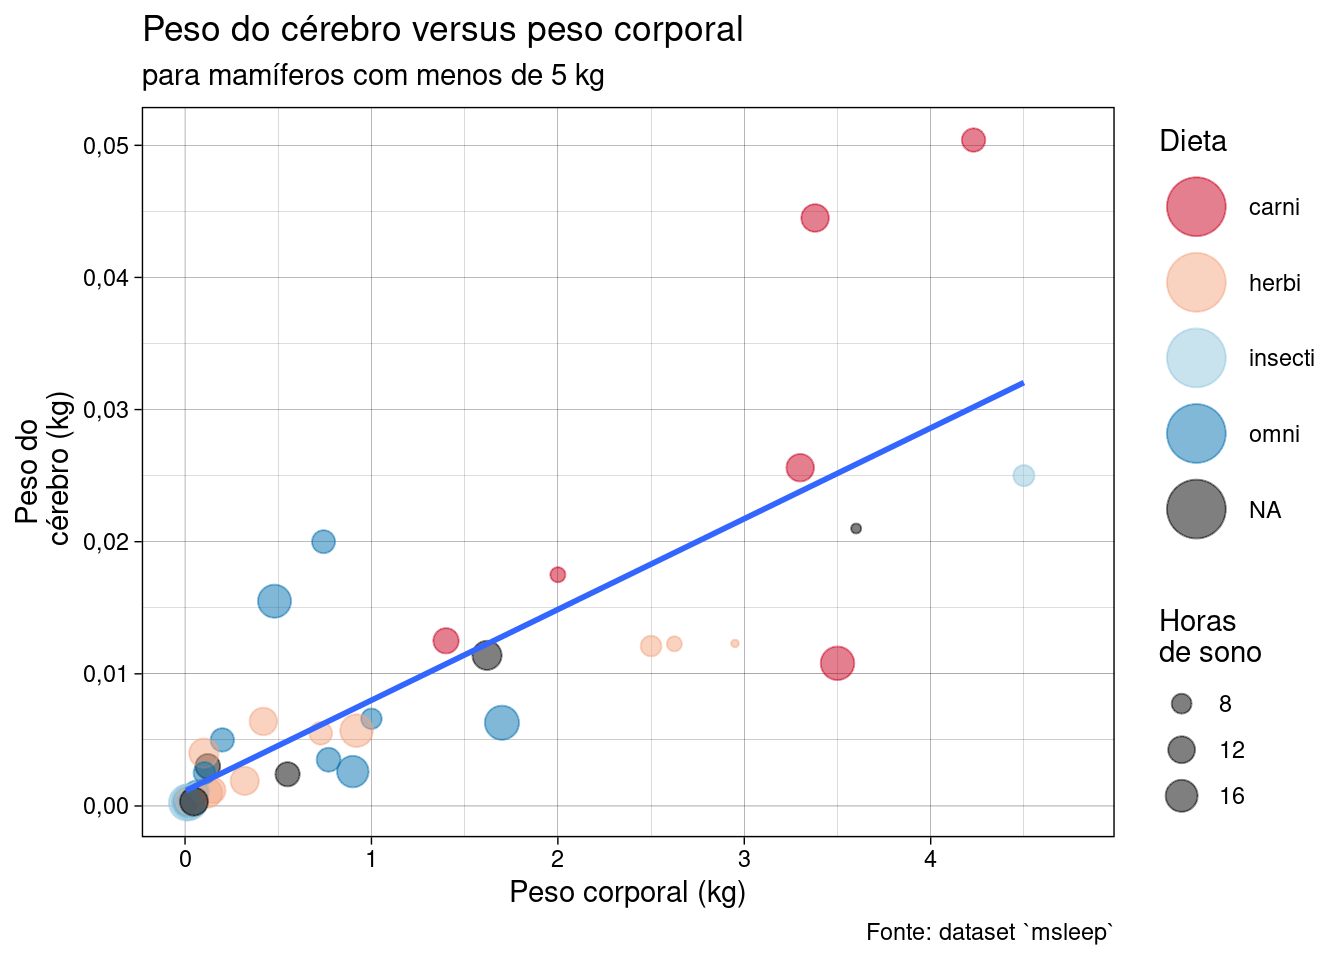
\includegraphics[width=1\linewidth]{_main_files/figure-latex/unnamed-chunk-115-1} \end{center}
\item
  A {\hl{caixa}} vai do valor do {\hl{primeiro quartil}} (embaixo) até o {\hl{terceiro quartil}} (em cima).
\item
  A {\hl{linha horizontal dentro da caixa}} representa o valor da {\hl{mediana}}.
\item
  As {\hl{linhas verticais}} acima e abaixo da caixa (pitorescamente chamadas de ``bigodes'') vão até o {\hl{limite inferior}} (primeiro quartil ${}- 1{,}5 \times \text{IQR}$) e até o {\hl{limite superior}} (terceiro quartil ${}+ 1{,}5 \times \text{IQR}$).
\item
  Neste \emph{boxplot}, não há \emph{outliers}.
\item
  \protect\hypertarget{onivoros}{}{} Podemos usar a posição $x$ para desenhar vários \emph{boxplots}, um para cada dieta:

\begin{Shaded}
\begin{Highlighting}[]
\NormalTok{sono }\SpecialCharTok{\%\textgreater{}\%} 
  \FunctionTok{ggplot}\NormalTok{(}\FunctionTok{aes}\NormalTok{(}\AttributeTok{x =}\NormalTok{ vore, }\AttributeTok{y =}\NormalTok{ sleep\_total)) }\SpecialCharTok{+}
    \FunctionTok{geom\_boxplot}\NormalTok{(}\AttributeTok{fill =} \StringTok{\textquotesingle{}gray\textquotesingle{}}\NormalTok{) }\SpecialCharTok{+}
    \FunctionTok{scale\_y\_continuous}\NormalTok{(}\AttributeTok{breaks =} \FunctionTok{seq}\NormalTok{(}\DecValTok{0}\NormalTok{, }\DecValTok{20}\NormalTok{, }\DecValTok{2}\NormalTok{))}
\end{Highlighting}
\end{Shaded}

  \begin{center}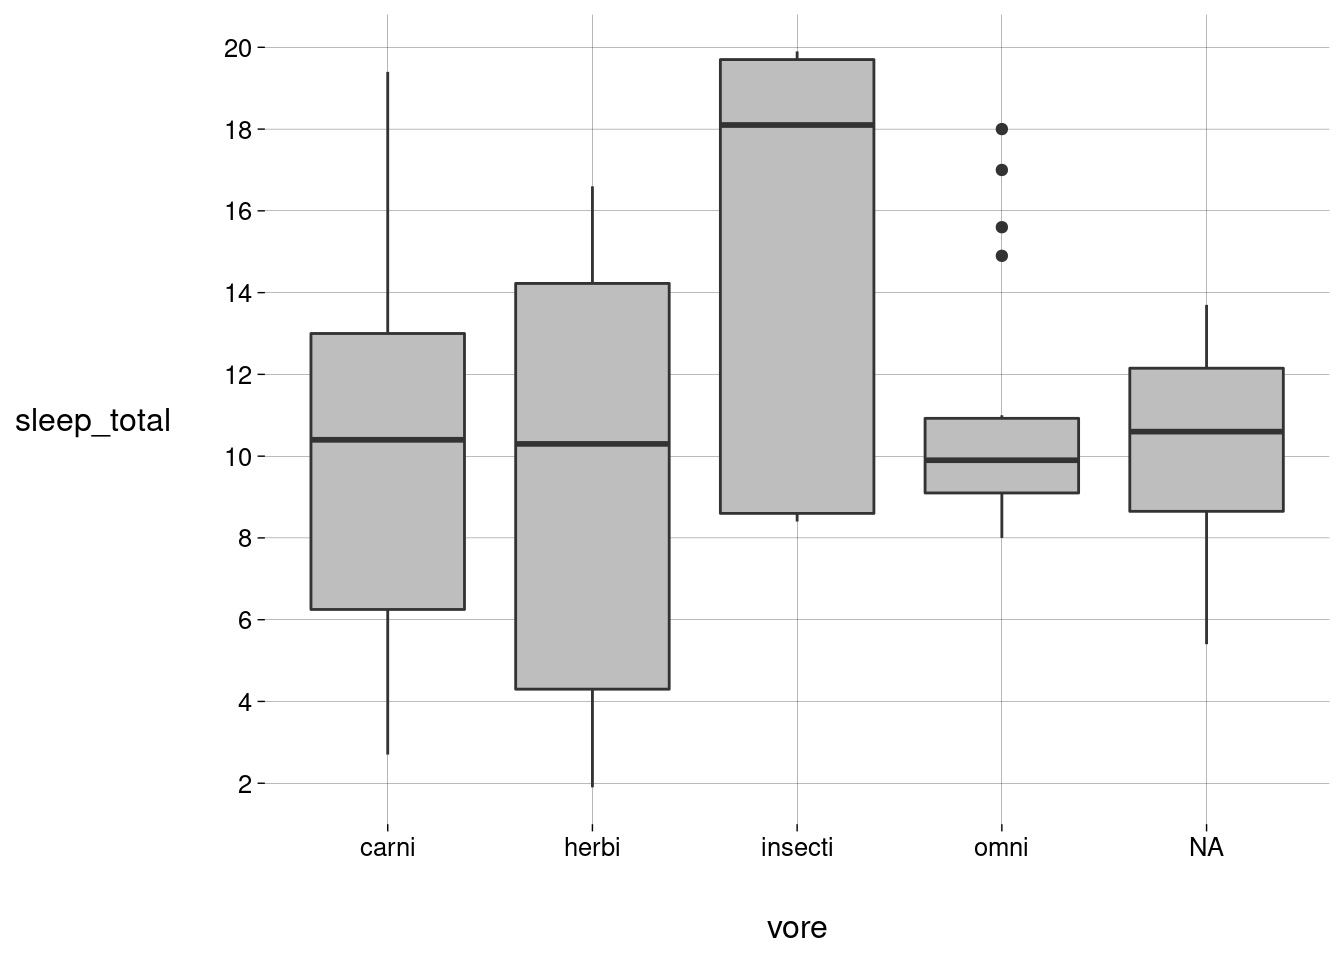
\includegraphics[width=1\linewidth]{_main_files/figure-latex/unnamed-chunk-116-1} \end{center}
\item
  No \emph{boxplot} de onívoros, {\hl{os \emph{outliers} aparecem como pontos isolados,}} acima da caixa, além dos alcances do bigode superior (aliás, onde está bigode superior?).
\item
  \emph{Boxplots} lado a lado são úteis para compararmos grupos diferentes de dados.
\item
  Veja como, com exceção dos insetívoros, as medianas dos grupos são parecidas.
\item
  Veja como carnívoros, insetívoros e herbívoros apresentam maior variação, enquanto onívoros e animais sem dieta registrada apresentam menor variação.
\item
  Vamos combinar, em um só gráfico

  \begin{itemize}
  \item
    Os pontos representando os animais,
  \item
    Os \emph{boxplots},
  \item
    As médias (que podem estar próximas ou distantes das medianas).
  \end{itemize}

\begin{Shaded}
\begin{Highlighting}[]
\NormalTok{sono }\SpecialCharTok{\%\textgreater{}\%} 
  \FunctionTok{ggplot}\NormalTok{(}\FunctionTok{aes}\NormalTok{(}\AttributeTok{x =}\NormalTok{ vore, }\AttributeTok{y =}\NormalTok{ sleep\_total)) }\SpecialCharTok{+}
    \FunctionTok{geom\_boxplot}\NormalTok{(}\AttributeTok{fill =} \StringTok{\textquotesingle{}gray\textquotesingle{}}\NormalTok{) }\SpecialCharTok{+}
    \FunctionTok{scale\_y\_continuous}\NormalTok{(}\AttributeTok{breaks =} \FunctionTok{seq}\NormalTok{(}\DecValTok{0}\NormalTok{, }\DecValTok{20}\NormalTok{, }\DecValTok{2}\NormalTok{)) }\SpecialCharTok{+}
    \FunctionTok{geom\_point}\NormalTok{(}
      \AttributeTok{color =} \StringTok{\textquotesingle{}blue\textquotesingle{}}\NormalTok{, }
      \AttributeTok{alpha =}\NormalTok{ .}\DecValTok{3}
\NormalTok{    ) }\SpecialCharTok{+}
    \FunctionTok{stat\_summary}\NormalTok{(}
      \AttributeTok{fun =}\NormalTok{ mean, }
      \AttributeTok{geom =} \StringTok{\textquotesingle{}point\textquotesingle{}}\NormalTok{, }
      \AttributeTok{color =} \StringTok{\textquotesingle{}red\textquotesingle{}}\NormalTok{, }
      \AttributeTok{shape =} \StringTok{\textquotesingle{}cross\textquotesingle{}}\NormalTok{, }
      \AttributeTok{size =} \DecValTok{5}\NormalTok{,}
      \AttributeTok{stroke =} \DecValTok{1}
\NormalTok{    ) }\SpecialCharTok{+}
    \FunctionTok{labs}\NormalTok{(}
      \AttributeTok{title =} \StringTok{\textquotesingle{}Sono total de diversos mamíferos, por dieta\textquotesingle{}}\NormalTok{,}
      \AttributeTok{subtitle =} \StringTok{\textquotesingle{}(o X vermelho representa a média)\textquotesingle{}}\NormalTok{,}
      \AttributeTok{x =} \StringTok{\textquotesingle{}dieta\textquotesingle{}}\NormalTok{,}
      \AttributeTok{y =} \StringTok{\textquotesingle{}sono total}\SpecialCharTok{\textbackslash{}n}\StringTok{(em horas)\textquotesingle{}}
\NormalTok{    )}
\end{Highlighting}
\end{Shaded}

  \begin{center}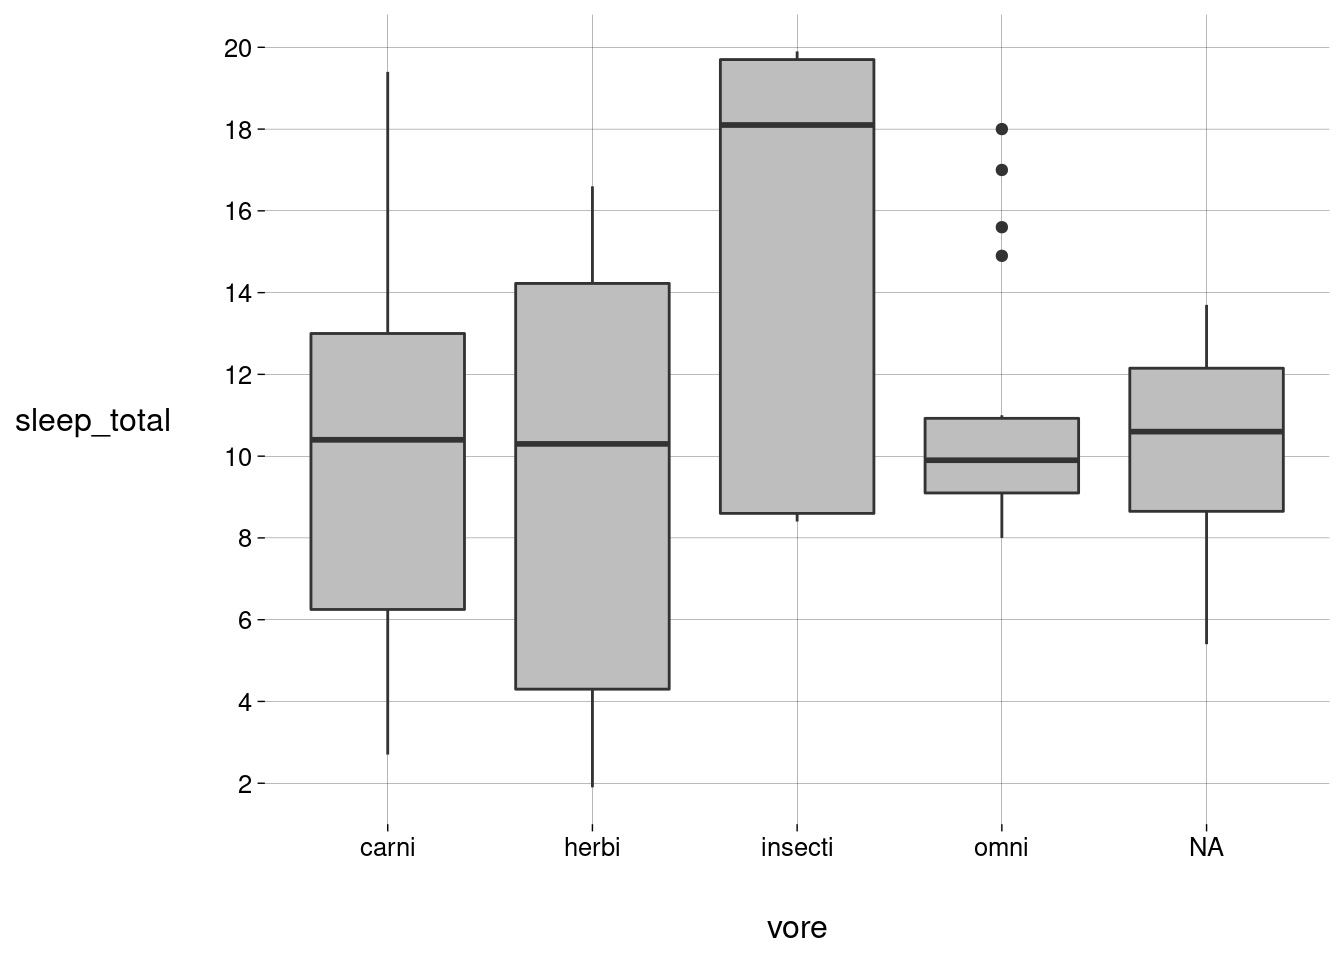
\includegraphics[width=1\linewidth]{_main_files/figure-latex/unnamed-chunk-117-1} \end{center}
\item
  {\hl{Quando a caixa é longa,}} o IQR é grande, e {\hl{os valores estão muito espalhados;}} é o caso dos herbívoros e insetívoros.
\item
  {\hl{Quando a caixa é curta,}} o IQR é pequeno, e {\hl{os valores estão pouco espalhados}}; é o caso dos onívoros. Como o IQR é pequeno, os $4$ mamíferos com mais de $14$ horas de sono são \emph{outliers}.
\item
  Observe, ainda, como os \emph{outliers} ``puxam'' a média dos onívoros para cima.
\end{itemize}

\hypertarget{vuxeddeo-2-2}{%
\section{Vídeo 2}\label{vuxeddeo-2-2}}

\begin{center} \url{https://youtu.be/QqnOvgBXJ-s} \end{center}

\hypertarget{gruxe1ficos-de-barras-e-de-colunas}{%
\section{Gráficos de barras e de colunas}\label{gruxe1ficos-de-barras-e-de-colunas}}

\hypertarget{conjunto-de-dados-1}{%
\subsection{Conjunto de dados}\label{conjunto-de-dados-1}}

\begin{itemize}
\item
  O R tem um \emph{array} de $3$ dimensões com dados sobre as cores dos cabelos e dos olhos de $592$ alunos e alunas de uma universidade americana em $1974$.
\item
  Se pedirmos para o R exibir os dados, veremos {\hl{duas matrizes}}, uma para cada sexo:

\begin{Shaded}
\begin{Highlighting}[]
\NormalTok{HairEyeColor}
\end{Highlighting}
\end{Shaded}

\begin{verbatim}
## , , Sex = Male
## 
##        Eye
## Hair    Brown Blue Hazel Green
##   Black    32   11    10     3
##   Brown    53   50    25    15
##   Red      10   10     7     7
##   Blond     3   30     5     8
## 
## , , Sex = Female
## 
##        Eye
## Hair    Brown Blue Hazel Green
##   Black    36    9     5     2
##   Brown    66   34    29    14
##   Red      16    7     7     7
##   Blond     4   64     5     8
\end{verbatim}
\item
  Vamos transformar este \emph{array} em um \emph{data frame}.
\item
  O \emph{array} contém apenas os totais de cada classe. Vamos usar a função \texttt{uncount} para gerar uma linha para cada aluno:

\begin{Shaded}
\begin{Highlighting}[]
\NormalTok{df\_orig }\OtherTok{\textless{}{-}} \FunctionTok{as.data.frame}\NormalTok{(HairEyeColor) }\SpecialCharTok{\%\textgreater{}\%} 
  \FunctionTok{uncount}\NormalTok{(Freq) }\SpecialCharTok{\%\textgreater{}\%} 
  \FunctionTok{as\_tibble}\NormalTok{()}

\NormalTok{df\_orig}
\end{Highlighting}
\end{Shaded}

\begin{verbatim}
## # A tibble: 592 x 3
##   Hair  Eye   Sex  
##   <fct> <fct> <fct>
## 1 Black Brown Male 
## 2 Black Brown Male 
## 3 Black Brown Male 
## 4 Black Brown Male 
## 5 Black Brown Male 
## 6 Black Brown Male 
## # ... with 586 more rows
\end{verbatim}
\item
  O \texttt{ggplot2} e os outros pacotes do \texttt{tidyverse} foram projetados para trabalhar com \emph{data frames} neste formato, {\hl{com uma observação (um indivíduo, um elemento) por linha.}} É o chamado {\hl{formato \emph{tidy}.}}
\item
  Usando vetores com elementos nomeados, podemos traduzir o conteúdo do \emph{data frame} para português:

\begin{Shaded}
\begin{Highlighting}[]
\NormalTok{cabelo }\OtherTok{\textless{}{-}} \FunctionTok{c}\NormalTok{(}
  \StringTok{\textquotesingle{}Brown\textquotesingle{}} \OtherTok{=} \StringTok{\textquotesingle{}castanhos\textquotesingle{}}\NormalTok{,}
  \StringTok{\textquotesingle{}Blond\textquotesingle{}} \OtherTok{=} \StringTok{\textquotesingle{}louros\textquotesingle{}}\NormalTok{,}
  \StringTok{\textquotesingle{}Black\textquotesingle{}} \OtherTok{=} \StringTok{\textquotesingle{}pretos\textquotesingle{}}\NormalTok{,}
  \StringTok{\textquotesingle{}Red\textquotesingle{}} \OtherTok{=} \StringTok{\textquotesingle{}ruivos\textquotesingle{}}
\NormalTok{)}

\NormalTok{olhos }\OtherTok{\textless{}{-}} \FunctionTok{c}\NormalTok{(}
  \StringTok{\textquotesingle{}Brown\textquotesingle{}} \OtherTok{=} \StringTok{\textquotesingle{}castanhos\textquotesingle{}}\NormalTok{,}
  \StringTok{\textquotesingle{}Blue\textquotesingle{}} \OtherTok{=} \StringTok{\textquotesingle{}azuis\textquotesingle{}}\NormalTok{,}
  \StringTok{\textquotesingle{}Hazel\textquotesingle{}} \OtherTok{=} \StringTok{\textquotesingle{}avelã\textquotesingle{}}\NormalTok{,}
  \StringTok{\textquotesingle{}Green\textquotesingle{}} \OtherTok{=} \StringTok{\textquotesingle{}verdes\textquotesingle{}}
\NormalTok{)}

\NormalTok{sexo }\OtherTok{\textless{}{-}} \FunctionTok{c}\NormalTok{(}
  \StringTok{\textquotesingle{}Male\textquotesingle{}} \OtherTok{=} \StringTok{\textquotesingle{}homem\textquotesingle{}}\NormalTok{,}
  \StringTok{\textquotesingle{}Female\textquotesingle{}} \OtherTok{=} \StringTok{\textquotesingle{}mulher\textquotesingle{}}
\NormalTok{)}

\NormalTok{df }\OtherTok{\textless{}{-}}\NormalTok{ df\_orig }\SpecialCharTok{\%\textgreater{}\%} 
  \FunctionTok{transmute}\NormalTok{(}
    \AttributeTok{cabelos =}\NormalTok{ cabelo[Hair],}
    \AttributeTok{olhos =}\NormalTok{ olhos[Eye],}
    \AttributeTok{sexo =}\NormalTok{ sexo[Sex]}
\NormalTok{  )}
\end{Highlighting}
\end{Shaded}
\item
  Um sumário:

\begin{Shaded}
\begin{Highlighting}[]
\NormalTok{df }\SpecialCharTok{\%\textgreater{}\%} \FunctionTok{dfSummary}\NormalTok{() }\SpecialCharTok{\%\textgreater{}\%} \FunctionTok{print}\NormalTok{()}
\end{Highlighting}
\end{Shaded}

  \begin{longtable}[]{@{}
    >{\raggedright\arraybackslash}p{(\columnwidth - 6\tabcolsep) * \real{0.1918}}
    >{\raggedright\arraybackslash}p{(\columnwidth - 6\tabcolsep) * \real{0.3425}}
    >{\raggedright\arraybackslash}p{(\columnwidth - 6\tabcolsep) * \real{0.3151}}
    >{\raggedright\arraybackslash}p{(\columnwidth - 6\tabcolsep) * \real{0.1507}}@{}}
  \toprule
  \begin{minipage}[b]{\linewidth}\raggedright
  Variável
  \end{minipage} & \begin{minipage}[b]{\linewidth}\raggedright
  Estatísticas / Valores
  \end{minipage} & \begin{minipage}[b]{\linewidth}\raggedright
  Freqs (\% de Válidos)
  \end{minipage} & \begin{minipage}[b]{\linewidth}\raggedright
  Faltante
  \end{minipage} \\
  \midrule
  \endhead
  \begin{minipage}[t]{\linewidth}\raggedright
  cabelos\\
  {[}character{]}\strut
  \end{minipage} & \begin{minipage}[t]{\linewidth}\raggedright
  1. castanhos\\
  2. louros\\
  3. pretos\\
  4. ruivos\strut
  \end{minipage} & \begin{minipage}[t]{\linewidth}\raggedright
  108 (18,2\%)\\
  286 (48,3\%)\\
  71 (12,0\%)\\
  127 (21,5\%)\strut
  \end{minipage} & \begin{minipage}[t]{\linewidth}\raggedright
  0\\
  (0,0\%)\strut
  \end{minipage} \\
  \begin{minipage}[t]{\linewidth}\raggedright
  olhos\\
  {[}character{]}\strut
  \end{minipage} & \begin{minipage}[t]{\linewidth}\raggedright
  1. avelã\\
  2. azuis\\
  3. castanhos\\
  4. verdes\strut
  \end{minipage} & \begin{minipage}[t]{\linewidth}\raggedright
  93 (15,7\%)\\
  215 (36,3\%)\\
  220 (37,2\%)\\
  64 (10,8\%)\strut
  \end{minipage} & \begin{minipage}[t]{\linewidth}\raggedright
  0\\
  (0,0\%)\strut
  \end{minipage} \\
  \begin{minipage}[t]{\linewidth}\raggedright
  sexo\\
  {[}character{]}\strut
  \end{minipage} & \begin{minipage}[t]{\linewidth}\raggedright
  1. homem\\
  2. mulher\strut
  \end{minipage} & \begin{minipage}[t]{\linewidth}\raggedright
  279 (47,1\%)\\
  313 (52,9\%)\strut
  \end{minipage} & \begin{minipage}[t]{\linewidth}\raggedright
  0\\
  (0,0\%)\strut
  \end{minipage} \\
  \bottomrule
  \end{longtable}
\end{itemize}

\hypertarget{gerando-gruxe1ficos-de-barras}{%
\subsection{Gerando gráficos de barras}\label{gerando-gruxe1ficos-de-barras}}

\begin{itemize}
\item
  Um {\hl{gráfico de barras}} contém uma barra para cada valor de uma {\hl{variável categórica.}}
\item
  {\hl{Usamos {\mbox{\texttt{geom\_bar}}} para gerar um gráfico de barras}} de cores de cabelo:

\begin{Shaded}
\begin{Highlighting}[]
\NormalTok{df }\SpecialCharTok{\%\textgreater{}\%} 
  \FunctionTok{ggplot}\NormalTok{(}\FunctionTok{aes}\NormalTok{(}\AttributeTok{x =}\NormalTok{ cabelos)) }\SpecialCharTok{+}
    \FunctionTok{geom\_bar}\NormalTok{() }\SpecialCharTok{+}
    \FunctionTok{labs}\NormalTok{(}\AttributeTok{y =} \ConstantTok{NULL}\NormalTok{)}
\end{Highlighting}
\end{Shaded}

  \begin{center}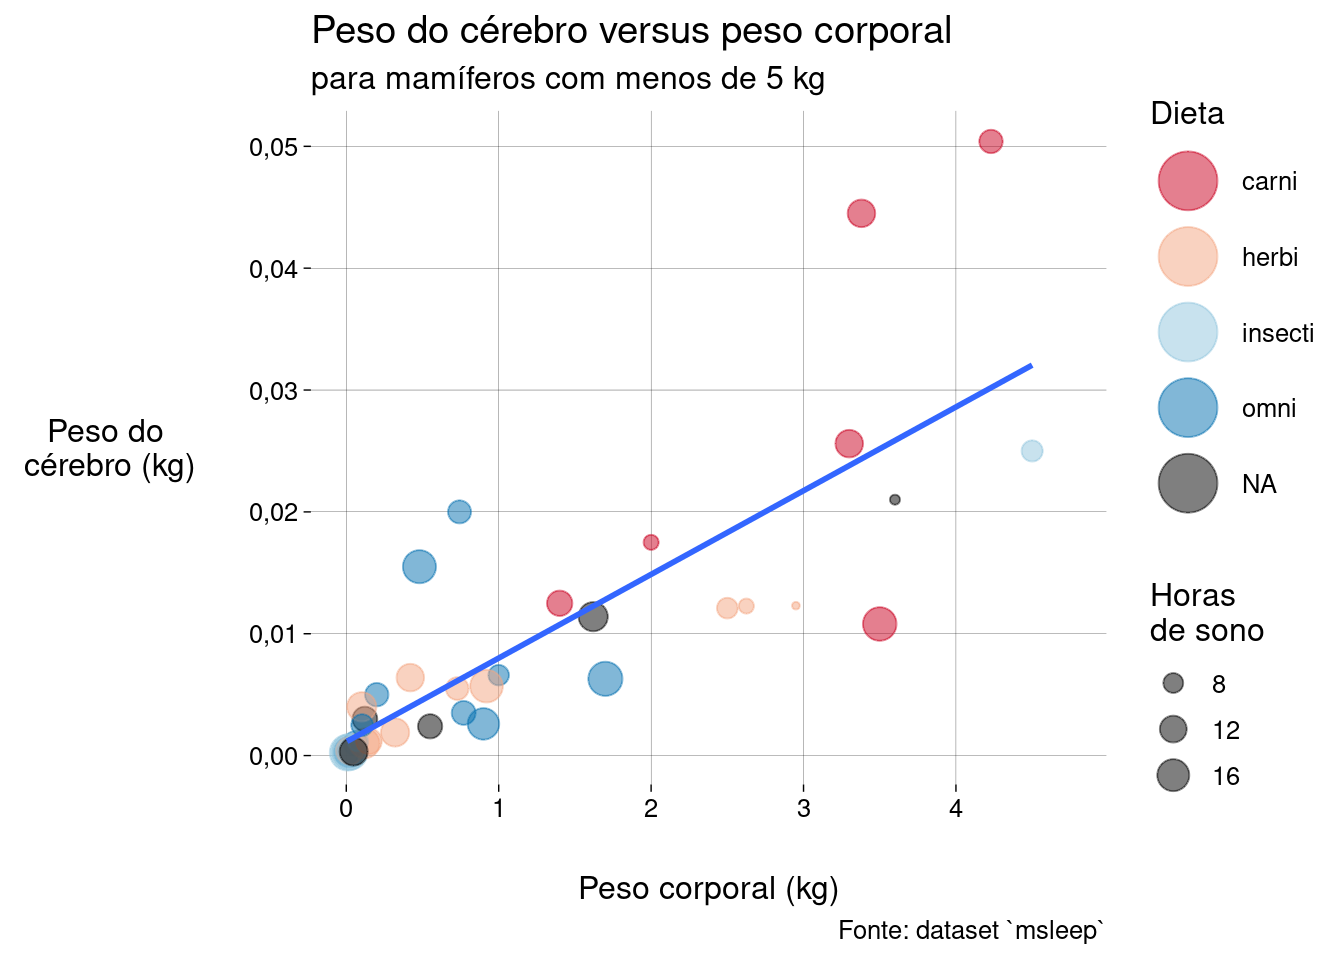
\includegraphics[width=1\linewidth]{_main_files/figure-latex/unnamed-chunk-123-1} \end{center}

  \begin{rmdimportant}

  \textbf{Gráfico de barras $\times$ histograma:}

  \begin{itemize}
  \item
    {\hl{Os dois tipos de gráficos mostram a frequência}} (quantidade de elementos) {\hl{no eixo vertical}}.
  \item
    No {\hl{gráfico de barras}}:

    \begin{itemize}
    \item
      A variável é {\hl{categórica}} (nominal).
    \item
      {\hl{Cada barra}} corresponde a {\hl{um valor}} da variável.
    \item
      {\hl{As barras não se tocam}}, enfatizando o fato de que a variável é categórica.
    \end{itemize}
  \item
    No {\hl{histograma}} (\protect\hyperlink{histograma1}{veja o exemplo}):

    \begin{itemize}
    \item
      A variável é {\hl{quantitativa}} (intervalar ou racional).
    \item
      {\hl{Cada barra}} corresponde a {\hl{uma classe de valores}} da variável.
    \item
      {\hl{As barras se tocam}}, para enfatizar que as classes são contíguas.
    \end{itemize}
  \end{itemize}

  \end{rmdimportant}
\item
  Um gráfico de barras é mais legível quando as barras são mostradas em ordem crescente ou decrescente.
\item
  Embora os valores da variável \texttt{cabelos} sejam \emph{strings}, podemos aplicar a eles funções que manipulam fatores.
\item
  A {\hl{função {\mbox{\texttt{fct\_infreq}}}}}, do pacote \texttt{forcats}, ordena os valores em {\hl{ordem decrescente de frequência}}.
\item
  A {\hl{função {\mbox{\texttt{fct\_rev}}}}}, também do pacote \texttt{forcats}, {\hl{inverte a ordenação.}}

\begin{Shaded}
\begin{Highlighting}[]
\NormalTok{df }\SpecialCharTok{\%\textgreater{}\%} 
  \FunctionTok{ggplot}\NormalTok{(}\FunctionTok{aes}\NormalTok{(}\AttributeTok{x =} \FunctionTok{fct\_rev}\NormalTok{(}\FunctionTok{fct\_infreq}\NormalTok{(cabelos)))) }\SpecialCharTok{+}
    \FunctionTok{geom\_bar}\NormalTok{() }\SpecialCharTok{+}
    \FunctionTok{labs}\NormalTok{(}
      \AttributeTok{x =} \StringTok{\textquotesingle{}cabelos\textquotesingle{}}\NormalTok{,}
      \AttributeTok{y =} \ConstantTok{NULL}
\NormalTok{    )}
\end{Highlighting}
\end{Shaded}

  \begin{center}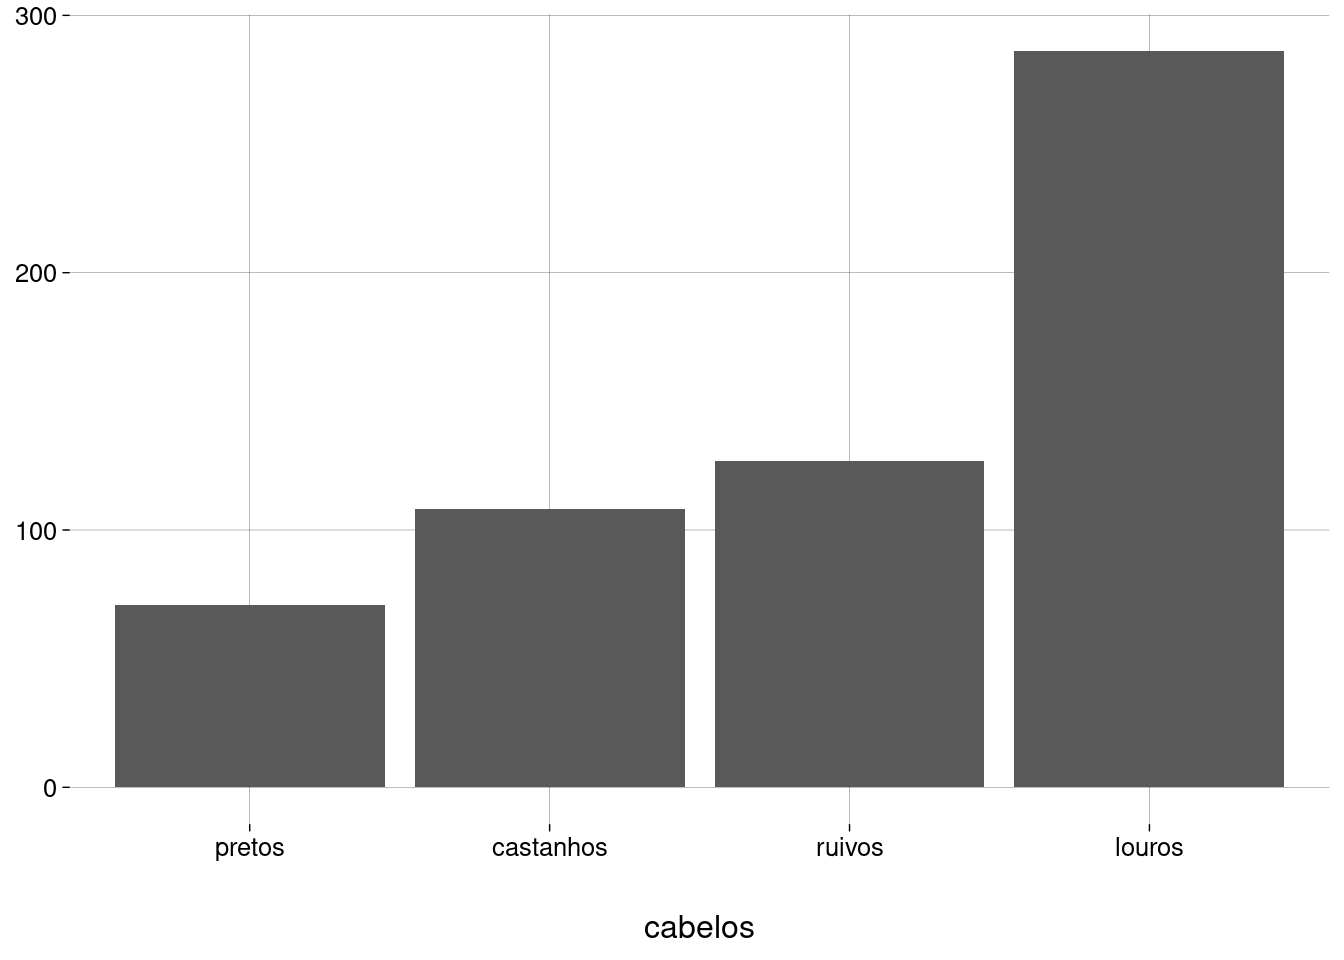
\includegraphics[width=1\linewidth]{_main_files/figure-latex/unnamed-chunk-124-1} \end{center}
\item
  A posição $x$ e a altura de cada barra são estéticas: {\hl{a posição $x$ representa a cor dos cabelos}}, e {\hl{a altura representa a frequência daquela cor}}.
\item
  Vamos acrescentar mais uma estética: {\hl{a cor de preenchimento vai representar o sexo}}.

\begin{Shaded}
\begin{Highlighting}[]
\NormalTok{df }\SpecialCharTok{\%\textgreater{}\%} 
  \FunctionTok{ggplot}\NormalTok{(}\FunctionTok{aes}\NormalTok{(}\AttributeTok{x =} \FunctionTok{fct\_rev}\NormalTok{(}\FunctionTok{fct\_infreq}\NormalTok{(cabelos)), }\AttributeTok{fill =}\NormalTok{ sexo)) }\SpecialCharTok{+}
    \FunctionTok{geom\_bar}\NormalTok{() }\SpecialCharTok{+}
    \FunctionTok{labs}\NormalTok{(}
      \AttributeTok{x =} \StringTok{\textquotesingle{}cabelos\textquotesingle{}}\NormalTok{,}
      \AttributeTok{y =} \ConstantTok{NULL}
\NormalTok{    )}
\end{Highlighting}
\end{Shaded}

  \begin{center}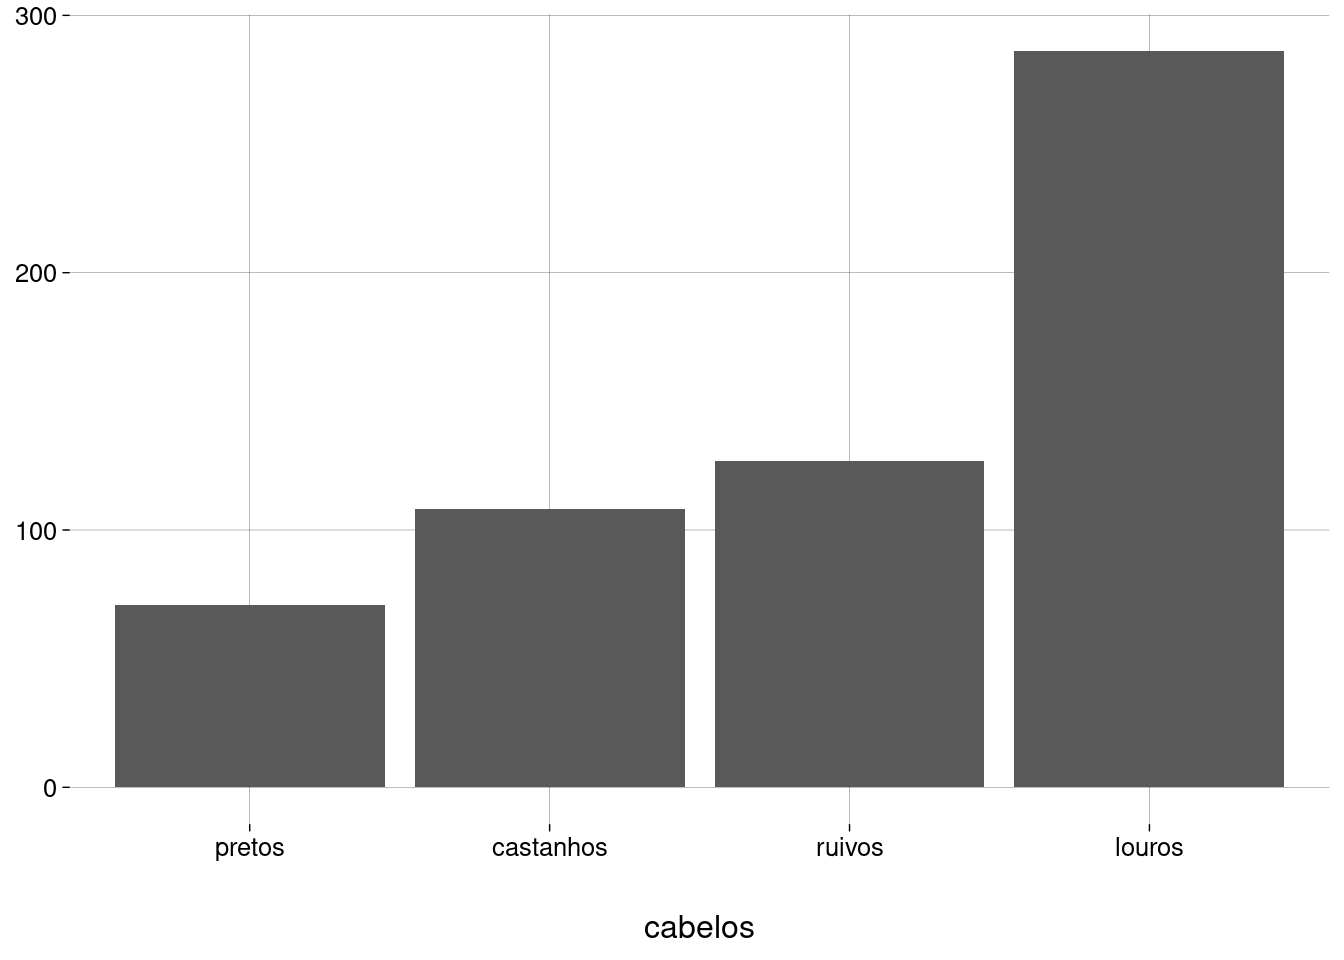
\includegraphics[width=1\linewidth]{_main_files/figure-latex/unnamed-chunk-125-1} \end{center}
\item
  Se a cor dos homens incomoda você, altere a escala que especifica o preenchimento (\texttt{scale\_fill\_discrete}):

\begin{Shaded}
\begin{Highlighting}[]
\NormalTok{df }\SpecialCharTok{\%\textgreater{}\%} 
  \FunctionTok{ggplot}\NormalTok{(}\FunctionTok{aes}\NormalTok{(}\AttributeTok{x =} \FunctionTok{fct\_rev}\NormalTok{(}\FunctionTok{fct\_infreq}\NormalTok{(cabelos)), }\AttributeTok{fill =}\NormalTok{ sexo)) }\SpecialCharTok{+}
    \FunctionTok{geom\_bar}\NormalTok{() }\SpecialCharTok{+}
    \FunctionTok{scale\_fill\_discrete}\NormalTok{(}\AttributeTok{type =} \FunctionTok{c}\NormalTok{(}\StringTok{\textquotesingle{}blue\textquotesingle{}}\NormalTok{, }\StringTok{\textquotesingle{}red\textquotesingle{}}\NormalTok{)) }\SpecialCharTok{+}
    \FunctionTok{labs}\NormalTok{(}
      \AttributeTok{x =} \StringTok{\textquotesingle{}cabelos\textquotesingle{}}\NormalTok{,}
      \AttributeTok{y =} \ConstantTok{NULL}
\NormalTok{    )}
\end{Highlighting}
\end{Shaded}

  \begin{center}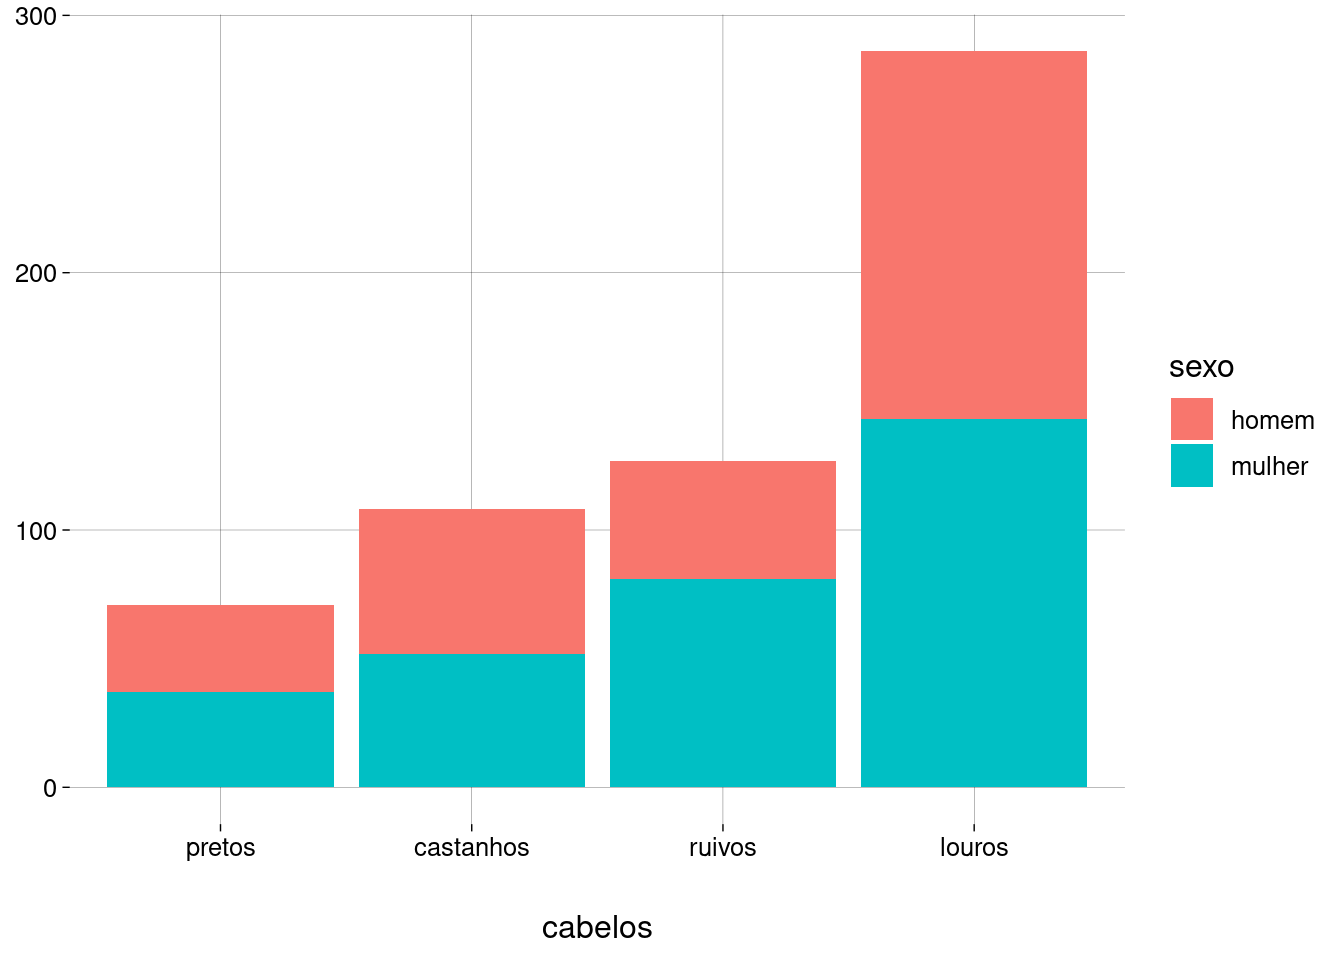
\includegraphics[width=1\linewidth]{_main_files/figure-latex/unnamed-chunk-126-1} \end{center}
\item
  {\hl{Podemos fazer um gráfico de barras horizontais com {\mbox{\texttt{coord\_flip}}}.}} Isto geralmente é útil quando os rótulos das barras são longos:

\begin{Shaded}
\begin{Highlighting}[]
\NormalTok{df }\SpecialCharTok{\%\textgreater{}\%} 
  \FunctionTok{ggplot}\NormalTok{(}\FunctionTok{aes}\NormalTok{(}\AttributeTok{x =} \FunctionTok{fct\_rev}\NormalTok{(}\FunctionTok{fct\_infreq}\NormalTok{(cabelos)), }\AttributeTok{fill =}\NormalTok{ sexo)) }\SpecialCharTok{+}
    \FunctionTok{geom\_bar}\NormalTok{() }\SpecialCharTok{+}
    \FunctionTok{scale\_fill\_discrete}\NormalTok{(}\AttributeTok{type =} \FunctionTok{c}\NormalTok{(}\StringTok{\textquotesingle{}blue\textquotesingle{}}\NormalTok{, }\StringTok{\textquotesingle{}red\textquotesingle{}}\NormalTok{)) }\SpecialCharTok{+}
    \FunctionTok{labs}\NormalTok{(}
      \AttributeTok{x =} \StringTok{\textquotesingle{}cabelos\textquotesingle{}}\NormalTok{,}
      \AttributeTok{y =} \ConstantTok{NULL}
\NormalTok{    ) }\SpecialCharTok{+}
    \FunctionTok{coord\_flip}\NormalTok{()}
\end{Highlighting}
\end{Shaded}

  \begin{center}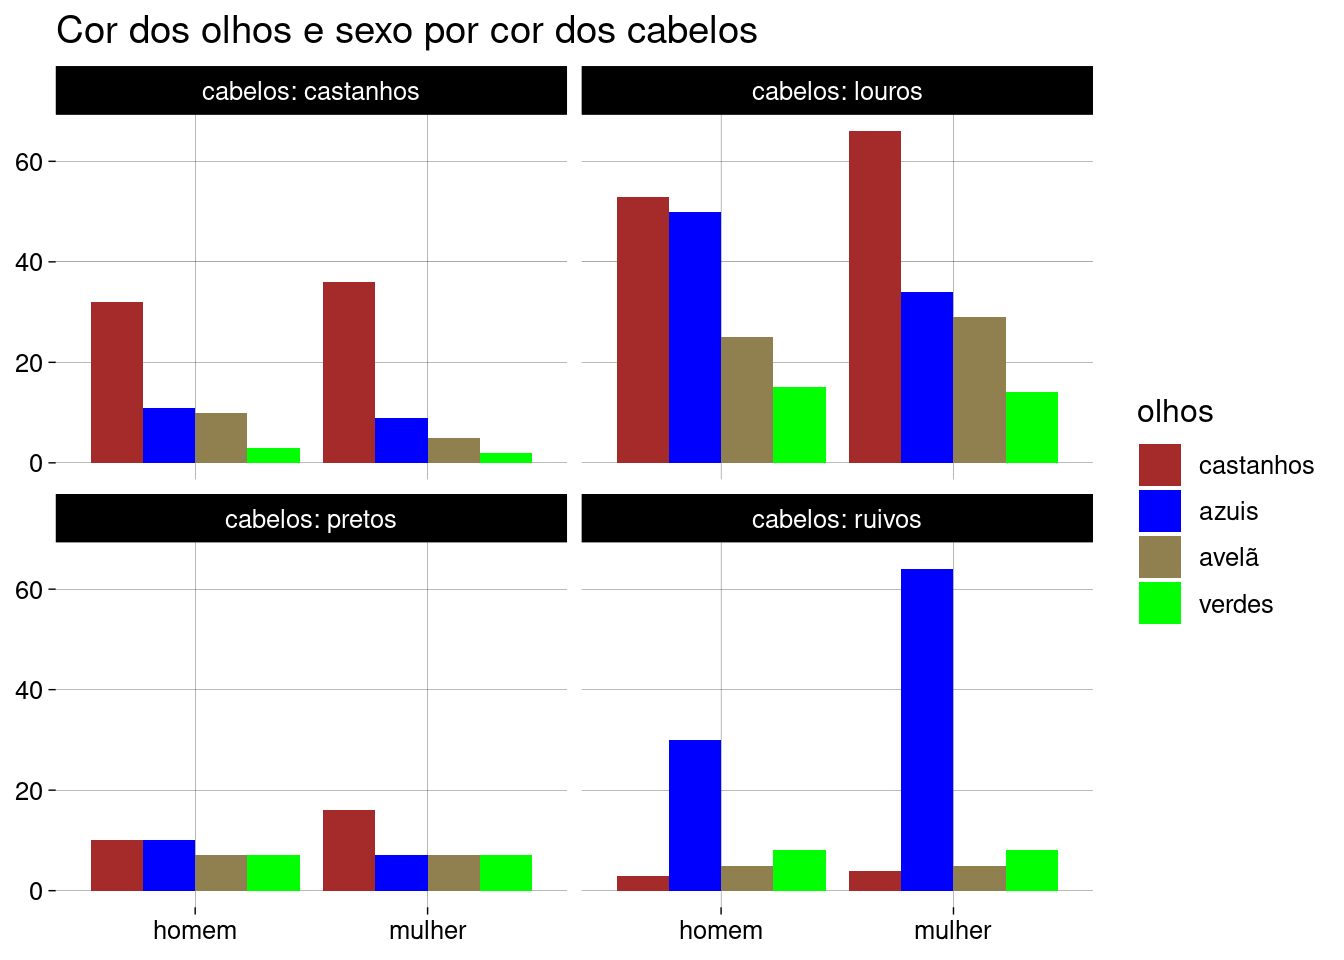
\includegraphics[width=1\linewidth]{_main_files/figure-latex/unnamed-chunk-127-1} \end{center}
\item
  Você consegue dizer se há mais homens ou mulheres com cabelos pretos? E castanhos? E ruivos?
\item
  Se posicionarmos as barras lado a lado, fica mais fácil responder.
\item
  Usamos o argumento \texttt{position\ =\ \textquotesingle{}dodge\textquotesingle{}} de \texttt{geom\_bar}. ``\emph{Dodge}'' significa ``esquivar-se'', em inglês.

\begin{Shaded}
\begin{Highlighting}[]
\NormalTok{df }\SpecialCharTok{\%\textgreater{}\%} 
  \FunctionTok{ggplot}\NormalTok{(}\FunctionTok{aes}\NormalTok{(}\AttributeTok{x =} \FunctionTok{fct\_rev}\NormalTok{(}\FunctionTok{fct\_infreq}\NormalTok{(cabelos)), }\AttributeTok{fill =}\NormalTok{ sexo)) }\SpecialCharTok{+}
    \FunctionTok{geom\_bar}\NormalTok{(}\AttributeTok{position =} \StringTok{\textquotesingle{}dodge\textquotesingle{}}\NormalTok{) }\SpecialCharTok{+}
    \FunctionTok{labs}\NormalTok{(}
      \AttributeTok{x =} \StringTok{\textquotesingle{}cabelos\textquotesingle{}}\NormalTok{,}
      \AttributeTok{y =} \ConstantTok{NULL}
\NormalTok{    ) }\SpecialCharTok{+}
    \FunctionTok{scale\_fill\_discrete}\NormalTok{(}\AttributeTok{type =} \FunctionTok{c}\NormalTok{(}\StringTok{\textquotesingle{}blue\textquotesingle{}}\NormalTok{, }\StringTok{\textquotesingle{}red\textquotesingle{}}\NormalTok{))}
\end{Highlighting}
\end{Shaded}

  \begin{center}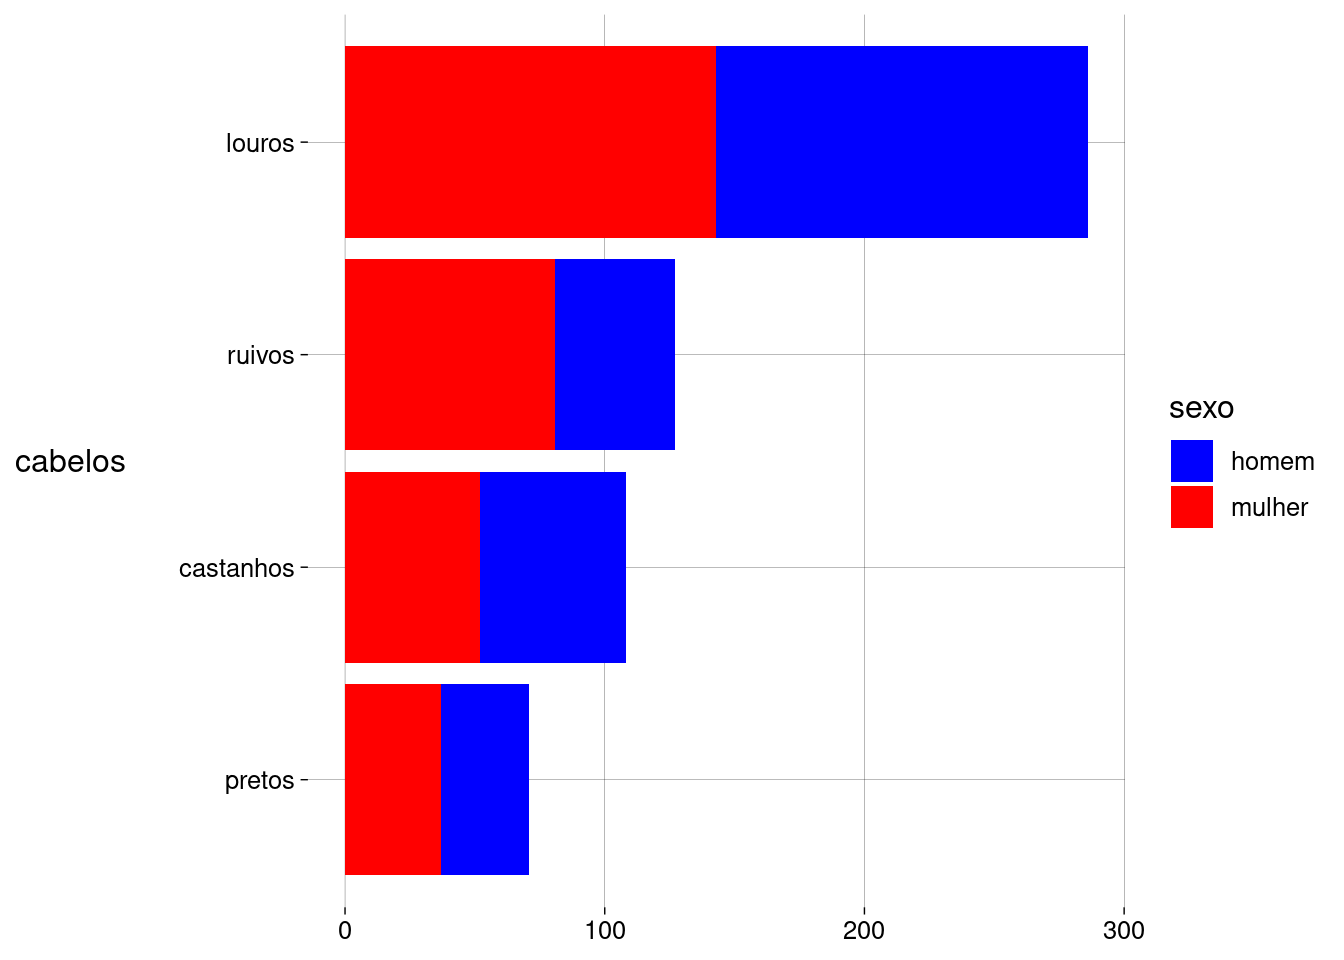
\includegraphics[width=1\linewidth]{_main_files/figure-latex/unnamed-chunk-128-1} \end{center}
\item
  Agora vamos examinar a relação entre as cores dos olhos e as cores dos cabelos:

\begin{Shaded}
\begin{Highlighting}[]
\NormalTok{df }\SpecialCharTok{\%\textgreater{}\%} 
  \FunctionTok{ggplot}\NormalTok{(}\FunctionTok{aes}\NormalTok{(}\AttributeTok{x =} \FunctionTok{fct\_rev}\NormalTok{(}\FunctionTok{fct\_infreq}\NormalTok{(cabelos)), }\AttributeTok{fill =}\NormalTok{ olhos)) }\SpecialCharTok{+}
    \FunctionTok{geom\_bar}\NormalTok{() }\SpecialCharTok{+}
    \FunctionTok{scale\_fill\_discrete}\NormalTok{(}
      \AttributeTok{type =} \FunctionTok{c}\NormalTok{(}\StringTok{\textquotesingle{}\#908050\textquotesingle{}}\NormalTok{, }\StringTok{\textquotesingle{}blue\textquotesingle{}}\NormalTok{, }\StringTok{\textquotesingle{}brown\textquotesingle{}}\NormalTok{, }\StringTok{\textquotesingle{}green\textquotesingle{}}\NormalTok{)}
\NormalTok{    ) }\SpecialCharTok{+}
    \FunctionTok{labs}\NormalTok{(}
      \AttributeTok{x =} \StringTok{\textquotesingle{}cabelos\textquotesingle{}}\NormalTok{,}
      \AttributeTok{y =} \ConstantTok{NULL}
\NormalTok{    )}
\end{Highlighting}
\end{Shaded}

  \begin{center}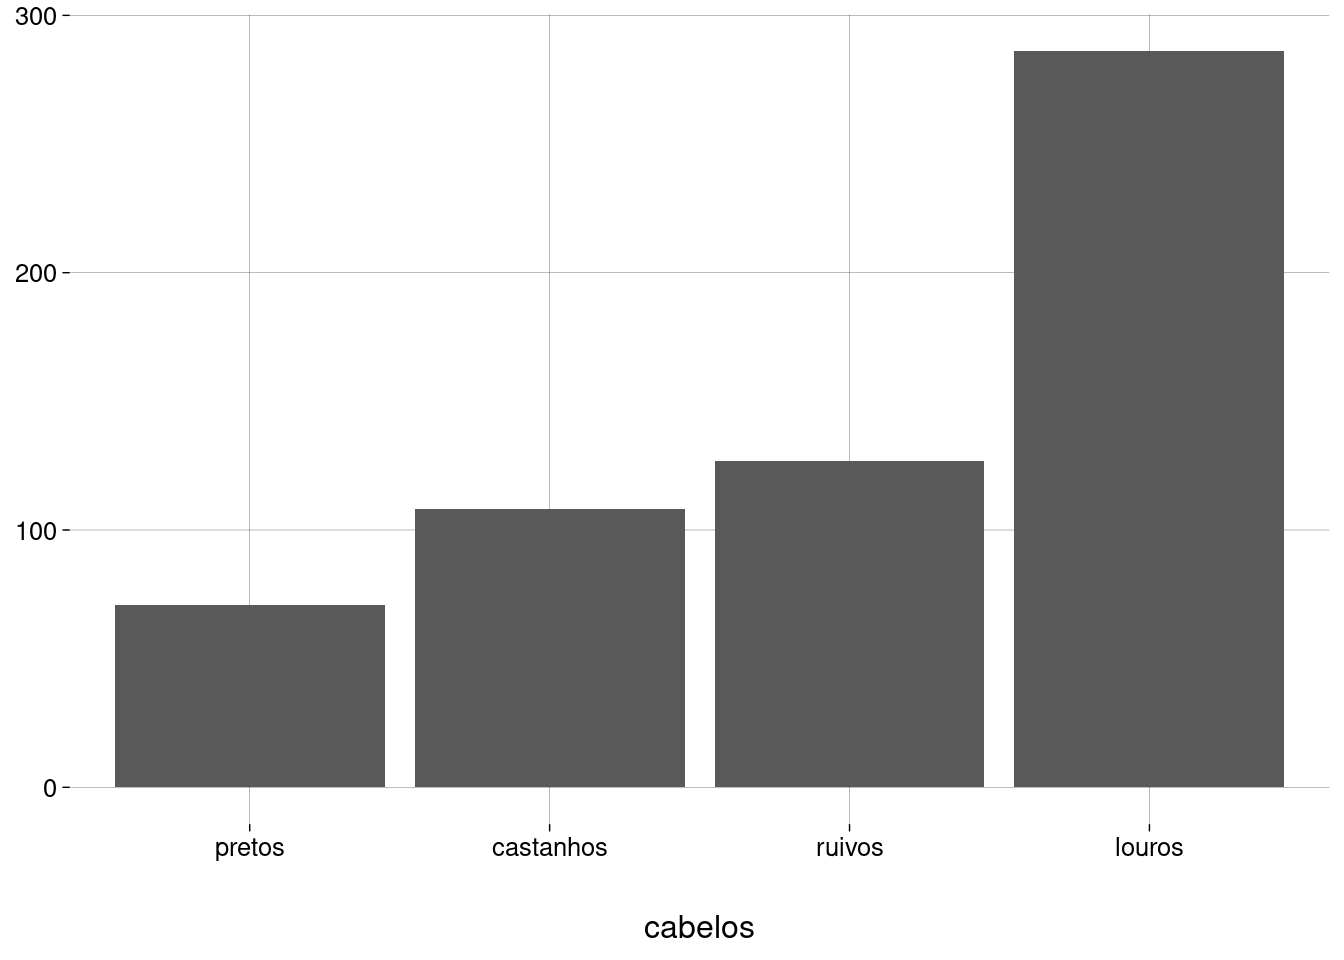
\includegraphics[width=1\linewidth]{_main_files/figure-latex/unnamed-chunk-129-1} \end{center}
\item
  Ou, com barras lado a lado:

\begin{Shaded}
\begin{Highlighting}[]
\NormalTok{df }\SpecialCharTok{\%\textgreater{}\%} 
  \FunctionTok{ggplot}\NormalTok{(}\FunctionTok{aes}\NormalTok{(}\AttributeTok{x =} \FunctionTok{fct\_rev}\NormalTok{(}\FunctionTok{fct\_infreq}\NormalTok{(cabelos)), }\AttributeTok{fill =}\NormalTok{ olhos)) }\SpecialCharTok{+}
    \FunctionTok{geom\_bar}\NormalTok{(}\AttributeTok{position =} \StringTok{\textquotesingle{}dodge\textquotesingle{}}\NormalTok{) }\SpecialCharTok{+}
    \FunctionTok{scale\_fill\_discrete}\NormalTok{(}
      \AttributeTok{type =} \FunctionTok{c}\NormalTok{(}\StringTok{\textquotesingle{}\#908050\textquotesingle{}}\NormalTok{, }\StringTok{\textquotesingle{}blue\textquotesingle{}}\NormalTok{, }\StringTok{\textquotesingle{}brown\textquotesingle{}}\NormalTok{, }\StringTok{\textquotesingle{}green\textquotesingle{}}\NormalTok{)}
\NormalTok{    ) }\SpecialCharTok{+}
    \FunctionTok{labs}\NormalTok{(}
      \AttributeTok{x =} \StringTok{\textquotesingle{}cabelos\textquotesingle{}}\NormalTok{,}
      \AttributeTok{y =} \ConstantTok{NULL}
\NormalTok{    )}
\end{Highlighting}
\end{Shaded}

  \begin{center}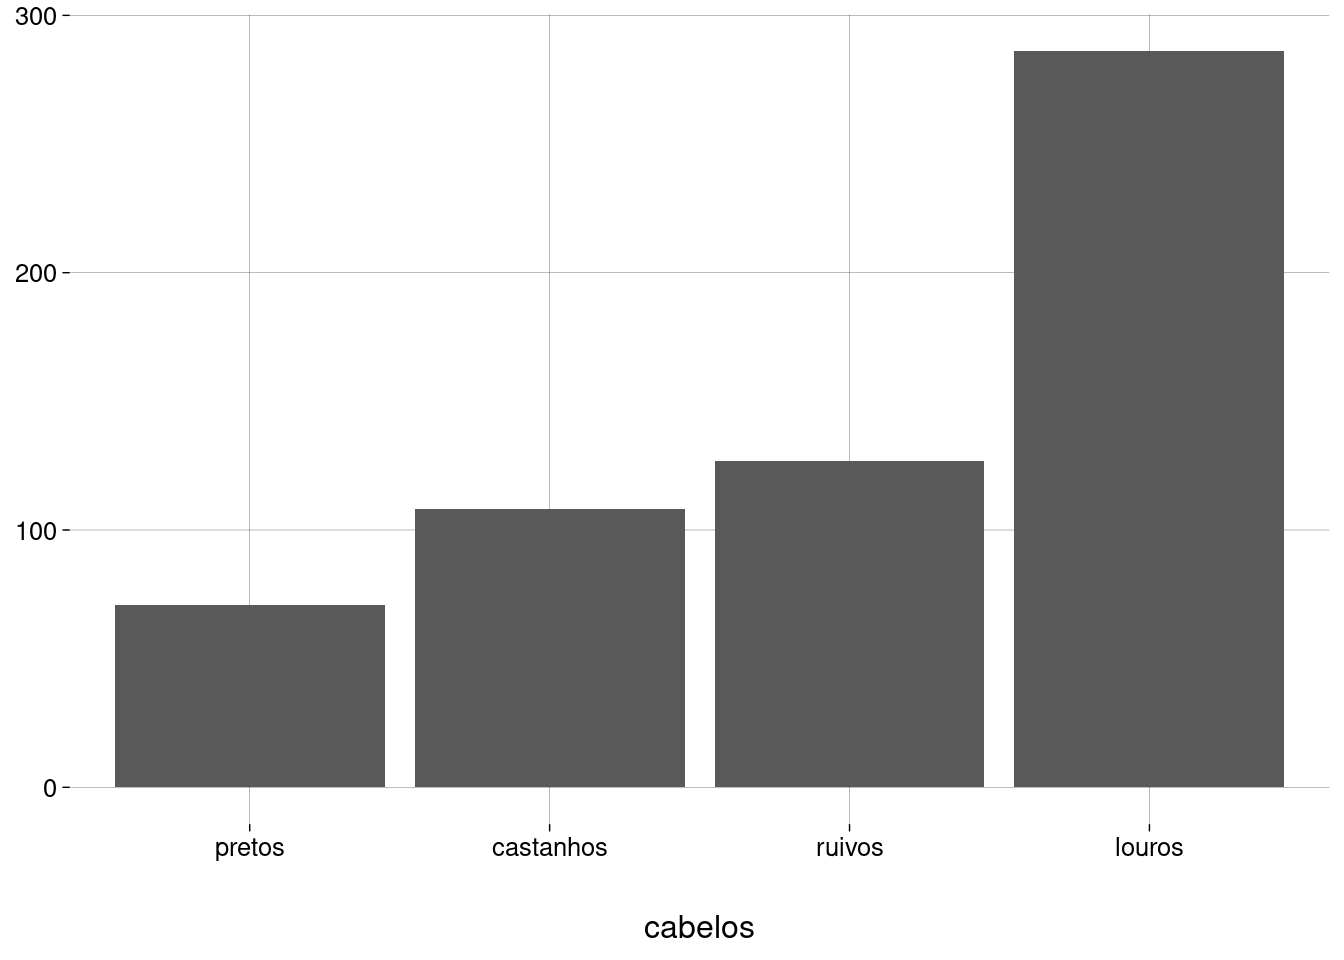
\includegraphics[width=1\linewidth]{_main_files/figure-latex/unnamed-chunk-130-1} \end{center}
\item
  Observações e perguntas:

  \begin{enumerate}
  \def\labelenumi{\arabic{enumi}.}
  \item
    Há mais pessoas louras de olhos castanhos do que louras de olhos azuis. O esperado não seria mais pessoas louras de olhos azuis? Pessoas louras de olhos castanhos pintaram os cabelos?
  \item
    Há muito mais ruivos de olhos azuis do que ruivos de olhos verdes. Não deveria ser o contrário? Também são pessoas que pintaram os cabelos de ruivo? Ou houve erro no registro das cores dos olhos?
  \end{enumerate}
\item
  Para incluir o sexo, podemos {\hl{facetar}} o gráfico. Usando \texttt{facet\_wrap}\footnote{O nome da variável segundo a qual facetar deve aparecer depois de um \texttt{\textasciitilde{}}.}, geramos dois subgráficos lado a lado:

\begin{Shaded}
\begin{Highlighting}[]
\NormalTok{df }\SpecialCharTok{\%\textgreater{}\%} 
  \FunctionTok{ggplot}\NormalTok{(}\FunctionTok{aes}\NormalTok{(}\AttributeTok{x =} \FunctionTok{fct\_rev}\NormalTok{(}\FunctionTok{fct\_infreq}\NormalTok{(cabelos)), }\AttributeTok{fill =}\NormalTok{ olhos)) }\SpecialCharTok{+}
    \FunctionTok{geom\_bar}\NormalTok{(}\AttributeTok{position =} \StringTok{\textquotesingle{}dodge\textquotesingle{}}\NormalTok{) }\SpecialCharTok{+}
    \FunctionTok{scale\_fill\_discrete}\NormalTok{(}\AttributeTok{type =} \FunctionTok{c}\NormalTok{(}\StringTok{\textquotesingle{}\#908050\textquotesingle{}}\NormalTok{, }\StringTok{\textquotesingle{}blue\textquotesingle{}}\NormalTok{, }\StringTok{\textquotesingle{}brown\textquotesingle{}}\NormalTok{, }\StringTok{\textquotesingle{}green\textquotesingle{}}\NormalTok{)) }\SpecialCharTok{+}
    \FunctionTok{facet\_wrap}\NormalTok{(}\SpecialCharTok{\textasciitilde{}}\NormalTok{sexo) }\SpecialCharTok{+}
    \FunctionTok{labs}\NormalTok{(}
      \AttributeTok{title =} \StringTok{\textquotesingle{}Cores de cabelos e olhos por sexo\textquotesingle{}}\NormalTok{,}
      \AttributeTok{y =} \ConstantTok{NULL}\NormalTok{,}
      \AttributeTok{x =} \StringTok{\textquotesingle{}cabelos\textquotesingle{}}
\NormalTok{    )}
\end{Highlighting}
\end{Shaded}

  \begin{center}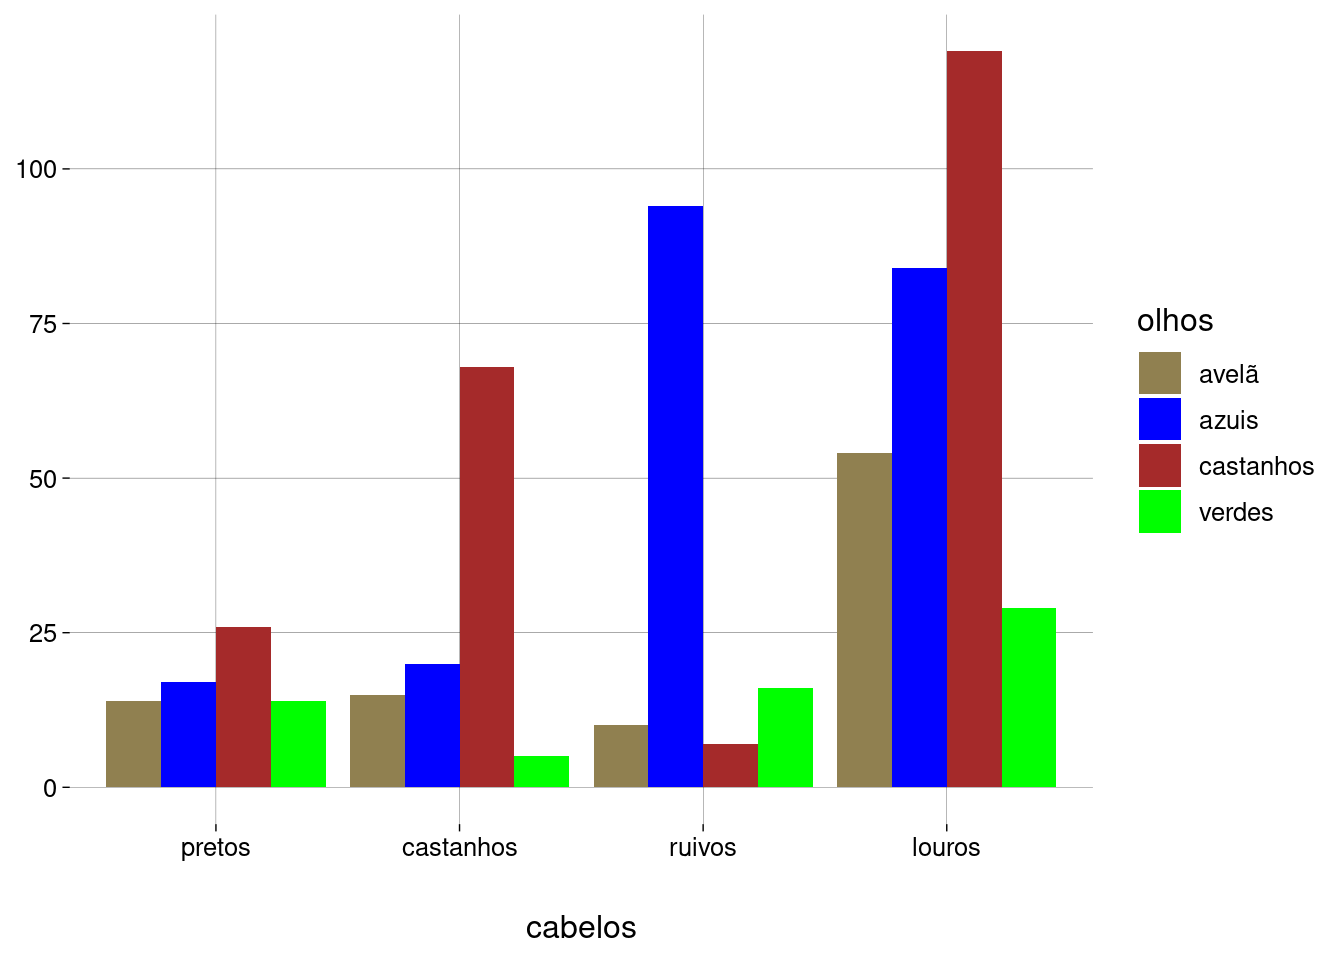
\includegraphics[width=1\linewidth]{_main_files/figure-latex/unnamed-chunk-131-1} \end{center}
\end{itemize}

\begin{itemize}
\item
  Se a quantidade grande de pessoas louras de olhos castanhos (em comparação com pessoas louras de olhos azuis) for por causa da pintura de cabelos, então o gráfico acima mostra que as mulheres pintam os cabelos de louro com mais frequência do que os homens.
\item
  Quando facetamos por cor de cabelos, também podemos observar as mesmas diferenças entre homens e mulheres:

\begin{Shaded}
\begin{Highlighting}[]
\NormalTok{df }\SpecialCharTok{\%\textgreater{}\%} 
  \FunctionTok{ggplot}\NormalTok{(}\FunctionTok{aes}\NormalTok{(}\AttributeTok{x =}\NormalTok{ sexo, }\AttributeTok{fill =} \FunctionTok{fct\_infreq}\NormalTok{(olhos))) }\SpecialCharTok{+}
    \FunctionTok{geom\_bar}\NormalTok{(}\AttributeTok{position =} \StringTok{\textquotesingle{}dodge\textquotesingle{}}\NormalTok{) }\SpecialCharTok{+}
    \FunctionTok{facet\_wrap}\NormalTok{(}\SpecialCharTok{\textasciitilde{}}\NormalTok{cabelos, }\AttributeTok{labeller =}\NormalTok{ label\_both) }\SpecialCharTok{+}
    \FunctionTok{scale\_fill\_discrete}\NormalTok{(}\AttributeTok{type =} \FunctionTok{c}\NormalTok{(}\StringTok{\textquotesingle{}brown\textquotesingle{}}\NormalTok{, }\StringTok{\textquotesingle{}blue\textquotesingle{}}\NormalTok{, }\StringTok{\textquotesingle{}\#908050\textquotesingle{}}\NormalTok{, }\StringTok{\textquotesingle{}green\textquotesingle{}}\NormalTok{)) }\SpecialCharTok{+}
    \FunctionTok{labs}\NormalTok{(}
      \AttributeTok{x =} \ConstantTok{NULL}\NormalTok{,}
      \AttributeTok{y =} \ConstantTok{NULL}\NormalTok{,}
      \AttributeTok{fill =} \StringTok{\textquotesingle{}olhos\textquotesingle{}}\NormalTok{,}
      \AttributeTok{title =} \StringTok{\textquotesingle{}Cor dos olhos e sexo por cor dos cabelos\textquotesingle{}}
\NormalTok{    )}
\end{Highlighting}
\end{Shaded}

  \begin{center}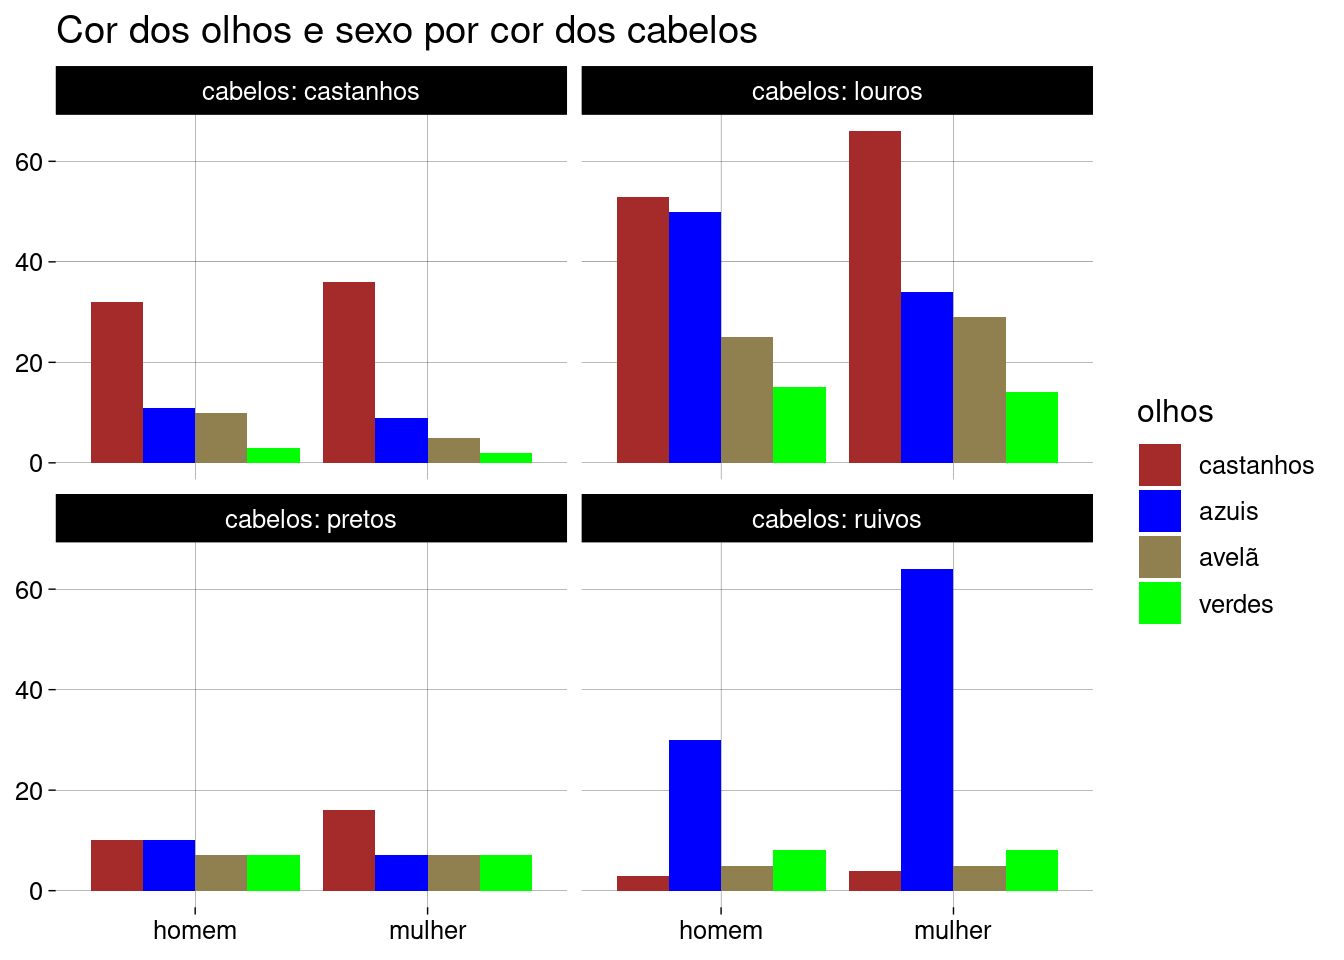
\includegraphics[width=1\linewidth]{_main_files/figure-latex/unnamed-chunk-132-1} \end{center}
\end{itemize}

\hypertarget{data-frame-juxe1-contendo-os-totais}{%
\subsection{\texorpdfstring{\emph{Data frame} já contendo os totais}{Data frame já contendo os totais}}\label{data-frame-juxe1-contendo-os-totais}}

\begin{itemize}
\item
  Você percebeu que {\hl{{\mbox{\texttt{geom\_bar}}} analisa o \emph{data frame} e calcula as frequências}} necessárias para construir o gráfico.
\item
  Em algumas situações, {\hl{o \emph{data frame} já contém as frequências}} (em vez de conter uma linha por indivíduo).
\item
  Vamos usar \texttt{count} para criar um \emph{data frame} assim:

\begin{Shaded}
\begin{Highlighting}[]
\NormalTok{df\_tot }\OtherTok{\textless{}{-}}\NormalTok{ df }\SpecialCharTok{\%\textgreater{}\%} 
  \FunctionTok{count}\NormalTok{(sexo, cabelos, olhos)}

\NormalTok{df\_tot}
\end{Highlighting}
\end{Shaded}

\begin{verbatim}
## # A tibble: 32 x 4
##   sexo  cabelos   olhos         n
##   <chr> <chr>     <chr>     <int>
## 1 homem castanhos avelã        10
## 2 homem castanhos azuis        11
## 3 homem castanhos castanhos    32
## 4 homem castanhos verdes        3
## 5 homem louros    avelã        25
## 6 homem louros    azuis        50
## # ... with 26 more rows
\end{verbatim}
\item
  Para $4$ cores de cabelo, $4$ cores de olhos, e $2$ sexos, são $32$ combinações possíveis.
\item
  Com este \emph{data frame}, podemos gerar todos os gráficos anteriores usando {\hl{{\mbox{\texttt{geom\_col}}} no lugar de {\mbox{\texttt{geom\_bar}}}}}. Por exemplo:

\begin{Shaded}
\begin{Highlighting}[]
\NormalTok{df\_tot }\SpecialCharTok{\%\textgreater{}\%} 
  \FunctionTok{ggplot}\NormalTok{(}\FunctionTok{aes}\NormalTok{(}\AttributeTok{x =}\NormalTok{ cabelos, }\AttributeTok{y =}\NormalTok{ n)) }\SpecialCharTok{+}
    \FunctionTok{geom\_col}\NormalTok{() }\SpecialCharTok{+}
    \FunctionTok{labs}\NormalTok{(}
      \AttributeTok{y =} \ConstantTok{NULL}
\NormalTok{    )}
\end{Highlighting}
\end{Shaded}

  \begin{center}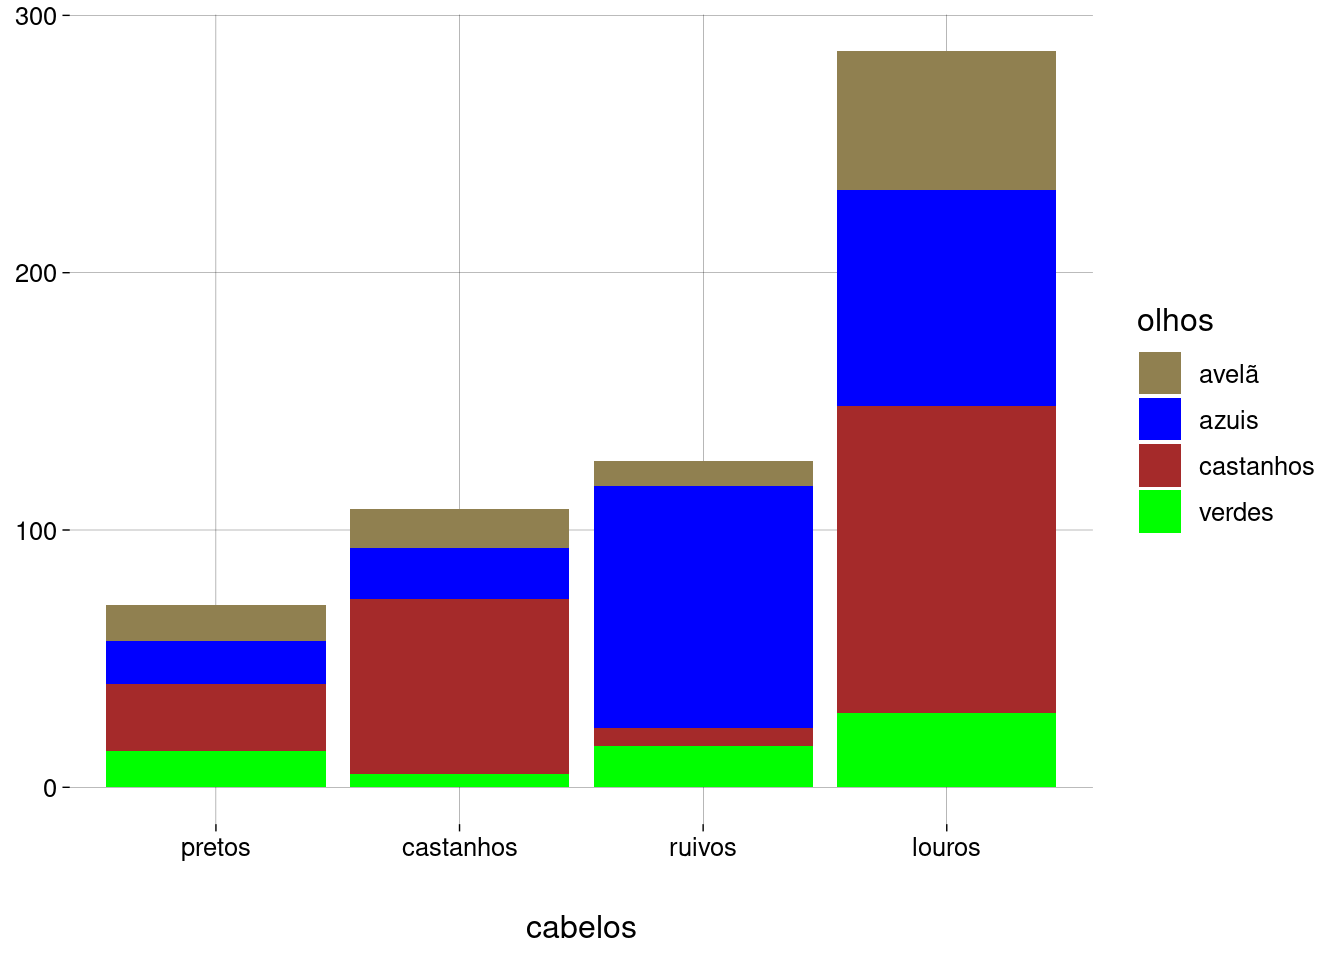
\includegraphics[width=1\linewidth]{_main_files/figure-latex/unnamed-chunk-134-1} \end{center}
\item
  Com \texttt{geom\_col}, {\hl{precisamos passar a estética $y$}} (no nosso exemplo, a variável \texttt{n}, que contém as frequências).
\item
  Para ordenar as barras, usamos a função \texttt{fct\_reorder}, que ordena os níveis de um fator (\texttt{cabelos}) de acordo com o resultado de uma função (\texttt{sum}) aplicada sobre os valores de outra variável (\texttt{n}):

\begin{Shaded}
\begin{Highlighting}[]
\NormalTok{df\_tot }\SpecialCharTok{\%\textgreater{}\%} 
  \FunctionTok{ggplot}\NormalTok{(}\FunctionTok{aes}\NormalTok{(}\AttributeTok{x =} \FunctionTok{fct\_reorder}\NormalTok{(cabelos, n, sum), }\AttributeTok{y =}\NormalTok{ n)) }\SpecialCharTok{+}
    \FunctionTok{geom\_col}\NormalTok{() }\SpecialCharTok{+}
    \FunctionTok{labs}\NormalTok{(}
      \AttributeTok{x =} \StringTok{\textquotesingle{}cabelos\textquotesingle{}}\NormalTok{,}
      \AttributeTok{y =} \ConstantTok{NULL}
\NormalTok{    )}
\end{Highlighting}
\end{Shaded}

  \begin{center}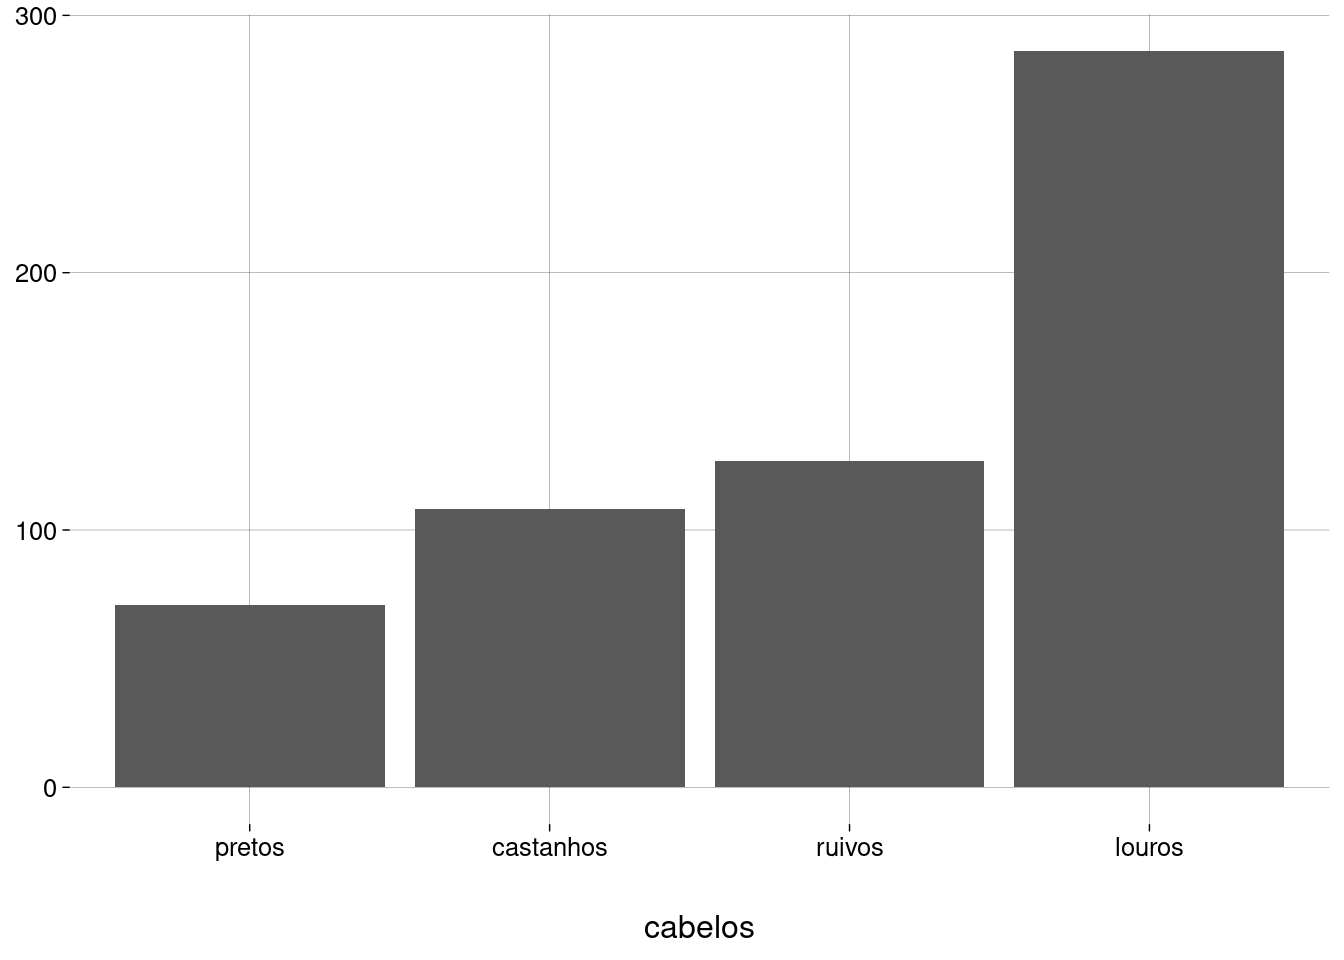
\includegraphics[width=1\linewidth]{_main_files/figure-latex/unnamed-chunk-135-1} \end{center}
\end{itemize}

\hypertarget{gruxe1ficos-de-linha-e-suxe9ries-temporais}{%
\section{Gráficos de linha e séries temporais}\label{gruxe1ficos-de-linha-e-suxe9ries-temporais}}

\hypertarget{conjunto-de-dados-2}{%
\subsection{Conjunto de dados}\label{conjunto-de-dados-2}}

\begin{itemize}
\item
  O R tem uma matriz com as quantidades de telefones em várias regiões do mundo ao longo de vários anos:

\begin{Shaded}
\begin{Highlighting}[]
\NormalTok{WorldPhones}
\end{Highlighting}
\end{Shaded}

\begin{verbatim}
##      N.Amer Europe Asia S.Amer Oceania Africa Mid.Amer
## 1951  45939  21574 2876   1815    1646     89      555
## 1956  60423  29990 4708   2568    2366   1411      733
## 1957  64721  32510 5230   2695    2526   1546      773
## 1958  68484  35218 6662   2845    2691   1663      836
## 1959  71799  37598 6856   3000    2868   1769      911
## 1960  76036  40341 8220   3145    3054   1905     1008
## 1961  79831  43173 9053   3338    3224   2005     1076
\end{verbatim}
\item
  Os números representam milhares.
\item
  {\hl{Os números dos anos são os nomes das linhas da matriz.}}
\item
  Vamos transformar esta matriz em uma \emph{tibble}:

\begin{Shaded}
\begin{Highlighting}[]
\NormalTok{fones }\OtherTok{\textless{}{-}}\NormalTok{ WorldPhones }\SpecialCharTok{\%\textgreater{}\%} 
  \FunctionTok{as\_tibble}\NormalTok{(}\AttributeTok{rownames =} \StringTok{\textquotesingle{}Ano\textquotesingle{}}\NormalTok{) }\SpecialCharTok{\%\textgreater{}\%} 
  \FunctionTok{mutate}\NormalTok{(}\AttributeTok{Ano =} \FunctionTok{as.numeric}\NormalTok{(Ano))}

\NormalTok{fones}
\end{Highlighting}
\end{Shaded}

\begin{verbatim}
## # A tibble: 7 x 8
##     Ano N.Amer Europe  Asia S.Amer Oceania Africa Mid.Amer
##   <dbl>  <dbl>  <dbl> <dbl>  <dbl>   <dbl>  <dbl>    <dbl>
## 1  1951  45939  21574  2876   1815    1646     89      555
## 2  1956  60423  29990  4708   2568    2366   1411      733
## 3  1957  64721  32510  5230   2695    2526   1546      773
## 4  1958  68484  35218  6662   2845    2691   1663      836
## 5  1959  71799  37598  6856   3000    2868   1769      911
## 6  1960  76036  40341  8220   3145    3054   1905     1008
## # ... with 1 more row
\end{verbatim}
\item
  Esta \emph{tibble} {\hl{não está no formato \emph{tidy}}}. Queremos que cada linha corresponda a uma observação, contendo

  \begin{itemize}
  \item
    Ano,
  \item
    Região,
  \item
    Quantidade de telefones.
  \end{itemize}
\item
  Usamos a função \texttt{pivot\_longer} para mudar o formato da \emph{tibble}:

\begin{Shaded}
\begin{Highlighting}[]
\NormalTok{fones\_long }\OtherTok{\textless{}{-}}\NormalTok{ fones }\SpecialCharTok{\%\textgreater{}\%} 
  \FunctionTok{pivot\_longer}\NormalTok{(}
    \AttributeTok{cols =} \SpecialCharTok{{-}}\NormalTok{Ano,}
    \AttributeTok{names\_to =} \StringTok{\textquotesingle{}Região\textquotesingle{}}\NormalTok{,}
    \AttributeTok{values\_to =} \StringTok{\textquotesingle{}n\textquotesingle{}}
\NormalTok{  )}

\NormalTok{fones\_long}
\end{Highlighting}
\end{Shaded}

\begin{verbatim}
## # A tibble: 49 x 3
##     Ano Região      n
##   <dbl> <chr>   <dbl>
## 1  1951 N.Amer  45939
## 2  1951 Europe  21574
## 3  1951 Asia     2876
## 4  1951 S.Amer   1815
## 5  1951 Oceania  1646
## 6  1951 Africa     89
## # ... with 43 more rows
\end{verbatim}
\item
  Confira: antes, tínhamos $7$ anos, com $7$ quantidades por ano, uma quantidade por região. Eram $49$ quantidades. Agora temos uma \emph{tibble} de $49$ linhas.
\end{itemize}

\hypertarget{gerando-gruxe1ficos-de-linha}{%
\subsection{Gerando gráficos de linha}\label{gerando-gruxe1ficos-de-linha}}

\begin{itemize}
\item
  {\hl{A geometria {\mbox{\texttt{geom\_line}}} gera gráficos de linha.}} Perceba como geramos uma linha por região:

\begin{Shaded}
\begin{Highlighting}[]
\NormalTok{fones\_long }\SpecialCharTok{\%\textgreater{}\%} 
  \FunctionTok{ggplot}\NormalTok{(}\FunctionTok{aes}\NormalTok{(}\AttributeTok{x =}\NormalTok{ Ano, }\AttributeTok{y =}\NormalTok{ n, }\AttributeTok{color =}\NormalTok{ Região)) }\SpecialCharTok{+}
    \FunctionTok{geom\_line}\NormalTok{() }\SpecialCharTok{+}
    \FunctionTok{scale\_x\_continuous}\NormalTok{(}\AttributeTok{breaks =} \DecValTok{1951}\SpecialCharTok{:}\DecValTok{1961}\NormalTok{)}
\end{Highlighting}
\end{Shaded}

  \begin{center}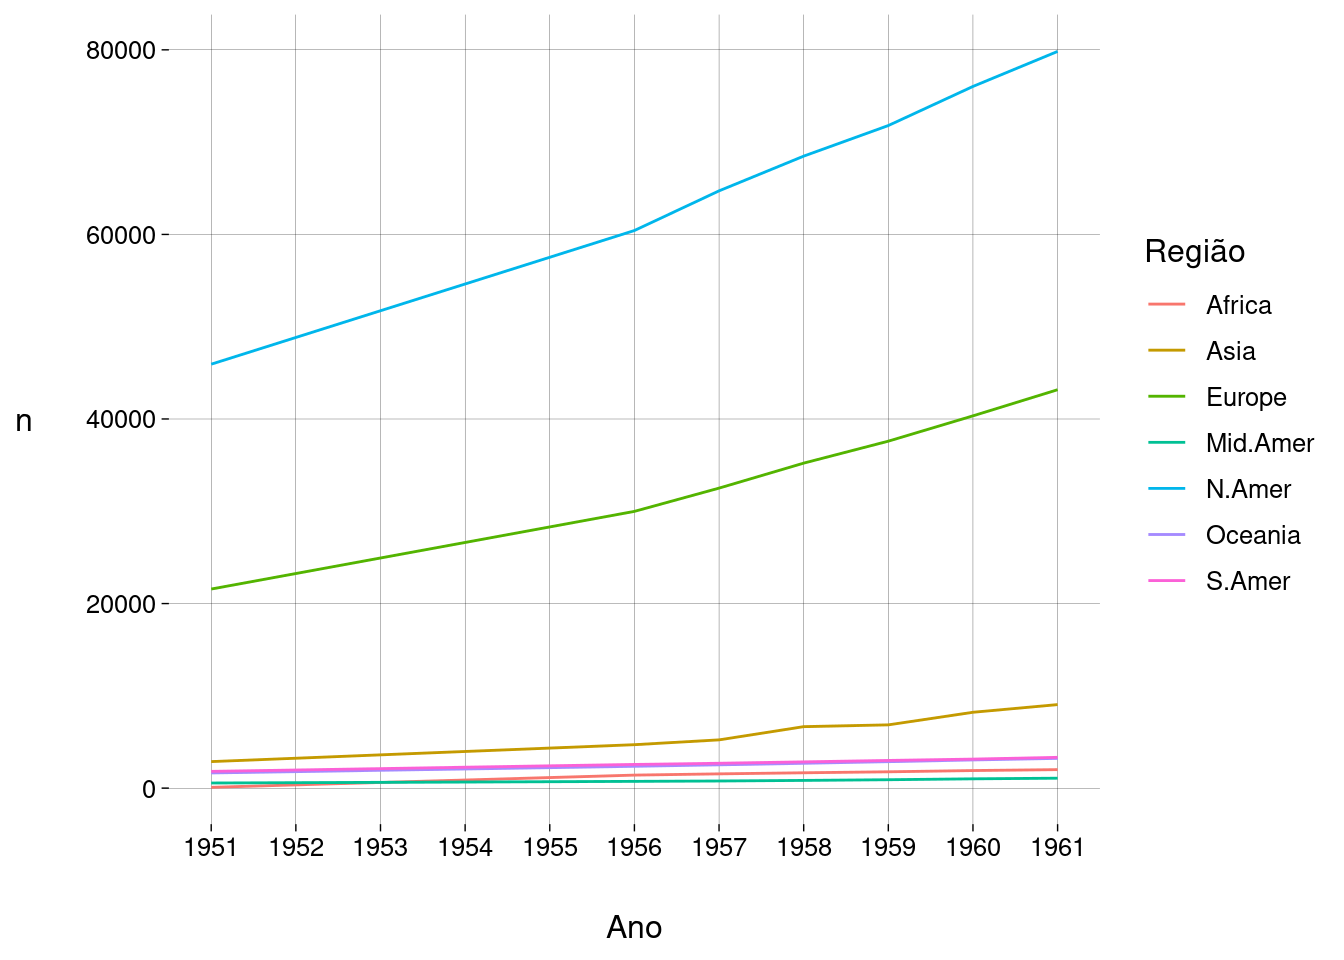
\includegraphics[width=1\linewidth]{_main_files/figure-latex/unnamed-chunk-139-1} \end{center}
\item
  Embora a legenda associe uma cor a cada região, {\hl{a leitura seria mais fácil se a ordem das regiões na legenda coincidisse com a posição das linhas na borda direita da grade}}:

\begin{Shaded}
\begin{Highlighting}[]
\NormalTok{fones\_long }\SpecialCharTok{\%\textgreater{}\%} 
  \FunctionTok{ggplot}\NormalTok{(}
      \FunctionTok{aes}\NormalTok{(}
        \AttributeTok{x =}\NormalTok{ Ano, }
        \AttributeTok{y =}\NormalTok{ n, }
        \AttributeTok{color =} \FunctionTok{fct\_rev}\NormalTok{(}\FunctionTok{fct\_reorder}\NormalTok{(Região, n, max))}
\NormalTok{      )}
\NormalTok{  ) }\SpecialCharTok{+}
    \FunctionTok{geom\_line}\NormalTok{() }\SpecialCharTok{+}
    \FunctionTok{scale\_x\_continuous}\NormalTok{(}\AttributeTok{breaks =} \DecValTok{1951}\SpecialCharTok{:}\DecValTok{1961}\NormalTok{) }\SpecialCharTok{+}
    \FunctionTok{labs}\NormalTok{(}
      \AttributeTok{color =} \StringTok{\textquotesingle{}Região\textquotesingle{}}\NormalTok{,}
      \AttributeTok{y =} \StringTok{\textquotesingle{}\textquotesingle{}}\NormalTok{,}
      \AttributeTok{x =} \ConstantTok{NULL}\NormalTok{,}
      \AttributeTok{title =} \StringTok{\textquotesingle{}Quantidade de aparelhos de telefone por ano, por região\textquotesingle{}}
\NormalTok{    )}
\end{Highlighting}
\end{Shaded}

  \begin{center}\includegraphics[width=1\linewidth]{_main_files/figure-latex/unnamed-chunk-140-1} \end{center}
\item
  Parece que está faltando uma linha, mas o que acontece é que as quantidades da América do Sul e da Oceania são bem parecidas:

\begin{Shaded}
\begin{Highlighting}[]
\NormalTok{fones\_long }\SpecialCharTok{\%\textgreater{}\%}
  \FunctionTok{filter}\NormalTok{(Região }\SpecialCharTok{\%in\%} \FunctionTok{c}\NormalTok{(}\StringTok{\textquotesingle{}S.Amer\textquotesingle{}}\NormalTok{, }\StringTok{\textquotesingle{}Oceania\textquotesingle{}}\NormalTok{)) }\SpecialCharTok{\%\textgreater{}\%} 
  \FunctionTok{ggplot}\NormalTok{(}
    \FunctionTok{aes}\NormalTok{(}
      \AttributeTok{x =}\NormalTok{ Ano, }
      \AttributeTok{y =}\NormalTok{ n, }
      \AttributeTok{color =} \FunctionTok{fct\_rev}\NormalTok{(}\FunctionTok{fct\_reorder}\NormalTok{(Região, n, max))}
\NormalTok{    )}
\NormalTok{  ) }\SpecialCharTok{+}
    \FunctionTok{geom\_line}\NormalTok{() }\SpecialCharTok{+}
    \FunctionTok{scale\_x\_continuous}\NormalTok{(}\AttributeTok{breaks =} \DecValTok{1951}\SpecialCharTok{:}\DecValTok{1961}\NormalTok{) }\SpecialCharTok{+}
    \FunctionTok{labs}\NormalTok{(}\AttributeTok{y =} \ConstantTok{NULL}\NormalTok{, }\AttributeTok{color =} \StringTok{\textquotesingle{}Região\textquotesingle{}}\NormalTok{)}
\end{Highlighting}
\end{Shaded}

  \begin{center}\includegraphics[width=1\linewidth]{_main_files/figure-latex/unnamed-chunk-141-1} \end{center}
\item
  Estamos tratando estes dados como simples números, mas, na verdade, {\hl{este conjunto de dados é uma série temporal (\emph{time series})}}.
\item
  R tem todo um conjunto de funções para tratar séries temporais, calcular tendências, achar padrões cíclicos, fazer estimativas, e gerar gráficos específicos, entre outras coisas.
\item
  Mas não vamos falar mais sobre séries temporais aqui.
\item
  O {\hl{pacote {\mbox{\texttt{tsibble}}}}} oferece maneiras de trabalhar com séries temporais de maneira \emph{tidy}. Você pode ler a documentação do pacote entrando

\begin{Shaded}
\begin{Highlighting}[]
\FunctionTok{library}\NormalTok{(tsibble)}
\NormalTok{?}\StringTok{\textasciigrave{}}\AttributeTok{tsibble{-}package}\StringTok{\textasciigrave{}}
\end{Highlighting}
\end{Shaded}
\end{itemize}

\hypertarget{exercuxedcios-6}{%
\section{Exercícios}\label{exercuxedcios-6}}

\hypertarget{o-bigode-dos-onuxedvoros}{%
\subsection{O bigode dos onívoros}\label{o-bigode-dos-onuxedvoros}}

\begin{itemize}
\tightlist
\item
  Examine o \emph{data frame} \texttt{sono} para descobrir o que houve com o bigode superior do \emph{boxplot} dos onívoros \protect\hyperlink{onivoros}{neste gráfico}.
\end{itemize}

\hypertarget{usando-geom_col}{%
\subsection{\texorpdfstring{Usando \texttt{geom\_col}}{Usando geom\_col}}\label{usando-geom_col}}

\begin{itemize}
\tightlist
\item
  Use \texttt{geom\_col} para reproduzir, a partir do \emph{data frame} \texttt{df\_tot}, todos os gráficos que foram gerados com \texttt{geom\_bar} na seção \protect\hyperlink{gerando-grux5cux25C3ux5cux25A1ficos-de-barras}{Gerando gráficos de barras}.
\end{itemize}

\hypertarget{section}{%
\subsection{}\label{section}}

\hypertarget{referuxeancias-sobre-visualizauxe7uxe3o-e-r}{%
\section{Referências sobre visualização e R}\label{referuxeancias-sobre-visualizauxe7uxe3o-e-r}}

\begin{rmdtip}
Busque mais informações sobre os pacotes \texttt{tidyverse} e \texttt{ggplot2} \protect\hyperlink{refrec}{nas referências recomendadas}.

\end{rmdtip}

\hypertarget{medidas}{%
\chapter{Medidas}\label{medidas}}

\hypertarget{vuxeddeo}{%
\section{Vídeo}\label{vuxeddeo}}

\begin{center} \url{https://youtu.be/C96MOP4YlaY} \end{center}

\hypertarget{medidas-de-centralidade}{%
\section{Medidas de centralidade}\label{medidas-de-centralidade}}

\hypertarget{muxe9dia}{%
\subsection{Média}\label{muxe9dia}}

\begin{itemize}
\item
  A {\hl{média de uma população}} é escrita como $\mu$, e é definida como
  \[\mu = \frac{\sum_{i=1}^N x_i}{N}\]

  \begin{itemize}
  \item
    $\sum_{i=1}^N x_i$ é a soma de todos os dados da população.
  \item
    $N$ é a quantidade de elementos na população.
  \end{itemize}
\item
  A {\hl{média de uma amostra}} é escrita como $\bar x$, e é definida como:
  \[\bar x = \frac{\sum_{i=1}^n x_i}{n}\]

  \begin{itemize}
  \item
    $\sum_{i=1}^n x_i$ é a soma de todos os dados da amostra.
  \item
    $n$ é a quantidade de elementos na amostra.
  \end{itemize}
\item
  O cálculo é essencialmente o mesmo. Só mudam os símbolos: $N$ versus $n$, e $\mu$ versus $\bar x$.
\end{itemize}

\hypertarget{exemplo}{%
\subsubsection{Exemplo}\label{exemplo}}

\begin{itemize}
\item
  Idades dos alunos de uma turma:

\begin{Shaded}
\begin{Highlighting}[]
\NormalTok{idades }\OtherTok{\textless{}{-}} \FunctionTok{c}\NormalTok{(}
  \DecValTok{20}\NormalTok{, }\DecValTok{20}\NormalTok{, }\DecValTok{20}\NormalTok{, }\DecValTok{20}\NormalTok{, }\DecValTok{20}\NormalTok{, }\DecValTok{20}\NormalTok{, }\DecValTok{21}\NormalTok{, }\DecValTok{21}\NormalTok{, }\DecValTok{21}\NormalTok{, }\DecValTok{21}\NormalTok{, }
  \DecValTok{22}\NormalTok{, }\DecValTok{22}\NormalTok{, }\DecValTok{22}\NormalTok{, }\DecValTok{23}\NormalTok{, }\DecValTok{23}\NormalTok{, }\DecValTok{23}\NormalTok{, }\DecValTok{23}\NormalTok{, }\DecValTok{24}\NormalTok{, }\DecValTok{24}\NormalTok{,}
  \DecValTok{65}
\NormalTok{)}
\end{Highlighting}
\end{Shaded}
\item
  Média {\hl{com}} o velhinho de $65$ anos:

\begin{Shaded}
\begin{Highlighting}[]
\FunctionTok{mean}\NormalTok{(idades)}
\end{Highlighting}
\end{Shaded}

\begin{verbatim}
## [1] 23,75
\end{verbatim}
\item
  Média {\hl{sem}} o velhinho:

\begin{Shaded}
\begin{Highlighting}[]
\FunctionTok{mean}\NormalTok{(idades[}\SpecialCharTok{{-}}\FunctionTok{length}\NormalTok{(idades)])}
\end{Highlighting}
\end{Shaded}

\begin{verbatim}
## [1] 21,57895
\end{verbatim}
\end{itemize}

\hypertarget{mediana-1}{%
\subsection{Mediana}\label{mediana-1}}

\begin{itemize}
\item
  Já aprendemos sobre a mediana na \protect\hyperlink{mediana}{seção sobre \emph{boxplots}}.
\item
  A idéia é que, depois de ordenar os dados, $50\%$ dos dados estarão à esquerda da mediana, e $50\%$ à direita.
\item
  A mediana não é tão sensível a \emph{outliers} quanto à média.
\end{itemize}

\hypertarget{exemplo-1}{%
\subsubsection{Exemplo}\label{exemplo-1}}

\begin{itemize}
\item
  Mediana {\hl{com}} o velhinho:

\begin{Shaded}
\begin{Highlighting}[]
\FunctionTok{median}\NormalTok{(idades)}
\end{Highlighting}
\end{Shaded}

\begin{verbatim}
## [1] 21,5
\end{verbatim}
\item
  Mediana {\hl{sem}} o velhinho:

\begin{Shaded}
\begin{Highlighting}[]
\FunctionTok{median}\NormalTok{(idades[}\SpecialCharTok{{-}}\FunctionTok{length}\NormalTok{(idades)])}
\end{Highlighting}
\end{Shaded}

\begin{verbatim}
## [1] 21
\end{verbatim}
\end{itemize}

\hypertarget{moda}{%
\subsection{Moda}\label{moda}}

\begin{itemize}
\item
  A {\hl{moda}} é o {\hl{valor mais frequente}} do conjunto de dados.
\item
  Pode haver mais de uma moda.
\item
  {\hl{Não existe uma função para a moda em R base.}} Por quê?
\item
  Por incrível que pareça, {\hl{é complicado definir a moda de forma a conseguir resultados interessantes}}.
\item
  {\hl{Por exemplo}}, vamos definir um conjunto de $1000$ valores numéricos distribuídos normalmente\footnote{Mais sobre a distribuição normal no capítulo ???.}, com média igual a $5$ e desvio-padrão\footnote{Mais sobre o desvio-padrão daqui a pouco.} igual a $2$:

\begin{Shaded}
\begin{Highlighting}[]
\NormalTok{normal }\OtherTok{\textless{}{-}} \FunctionTok{rnorm}\NormalTok{(}\DecValTok{1000}\NormalTok{, }\AttributeTok{mean =} \DecValTok{5}\NormalTok{, }\AttributeTok{sd =} \DecValTok{2}\NormalTok{)}
\end{Highlighting}
\end{Shaded}
\item
  \protect\hypertarget{dados-normais}{}{} O histograma dos nossos dados é

  \begin{center}\includegraphics[width=1\linewidth]{_main_files/figure-latex/unnamed-chunk-146-1} \end{center}
\item
  Vamos calcular a moda com a função \texttt{mfv} (\emph{most frequent value}), do pacote \texttt{modeest}:

\begin{Shaded}
\begin{Highlighting}[]
\CommentTok{\# Pacote com funções para calcular modas}
\FunctionTok{library}\NormalTok{(modeest)}
\end{Highlighting}
\end{Shaded}

\begin{verbatim}
## Registered S3 method overwritten by 'rmutil':
##   method         from
##   print.response httr
\end{verbatim}

\begin{Shaded}
\begin{Highlighting}[]
\CommentTok{\# Por causa de um bug na função mfv, }
\CommentTok{\# precisamos de números com ponto decimal}
\CommentTok{\# (em vez de vírgula):}
\FunctionTok{options}\NormalTok{(}\AttributeTok{OutDec =} \StringTok{\textquotesingle{}.\textquotesingle{}}\NormalTok{)}
\FunctionTok{mfv}\NormalTok{(normal)}
\end{Highlighting}
\end{Shaded}

\begin{verbatim}
##    [1] -0.474763335 -0.397280721 -0.143228292 -0.123519774 -0.053089822
##    [6] -0.000208636  0.265914440  0.467862897  0.592128087  0.647387675
##   [11]  0.718079212  0.729847819  0.778130124  0.790265222  0.806860891
##   [16]  0.862311390  0.914416238  0.921510323  1.037663354  1.078820606
##   [21]  1.121696568  1.128389959  1.143496592  1.224604349  1.233851191
##   [26]  1.236787398  1.255303842  1.285752312  1.366759493  1.389271780
##   [31]  1.437239398  1.449979570  1.458924669  1.463548376  1.472782925
##   [36]  1.475083361  1.482299047  1.524287968  1.528464953  1.542881662
##   [41]  1.558148057  1.565709395  1.597846940  1.599545621  1.610347720
##   [46]  1.657075198  1.668364206  1.685075092  1.720075976  1.730192814
##   [51]  1.731447548  1.788536426  1.790507633  1.793665979  1.799574408
##   [56]  1.818739880  1.838495902  1.840637261  1.854664368  1.868524229
##   [61]  1.870770189  1.897558862  1.959183764  1.960951682  1.971686965
##   [66]  1.982298976  1.992136687  1.995344960  2.017571137  2.023424615
##   [71]  2.026558337  2.034974228  2.037000329  2.055580000  2.059999504
##   [76]  2.060266712  2.062350134  2.063183780  2.068185690  2.099828550
##   [81]  2.139988638  2.148529564  2.159248443  2.172697775  2.198719235
##   [86]  2.199191490  2.203119486  2.206660366  2.207389059  2.208659500
##   [91]  2.210705097  2.210815915  2.215962554  2.218738075  2.226433776
##   [96]  2.248105317  2.248997300  2.269910075  2.275926220  2.295960293
##  [101]  2.297981951  2.303813581  2.333069167  2.345689201  2.414131767
##  [106]  2.430772859  2.450757541  2.455083760  2.468317534  2.473074805
##  [111]  2.478428884  2.478758459  2.487955600  2.517798905  2.537985289
##  [116]  2.542165033  2.545168756  2.557013771  2.567739046  2.580230730
##  [121]  2.594099965  2.607398154  2.609617142  2.640391152  2.644808421
##  [126]  2.663535140  2.664684539  2.665137348  2.671918147  2.697595633
##  [131]  2.700782152  2.706189989  2.715124749  2.747685134  2.750185782
##  [136]  2.750621716  2.753581351  2.774289507  2.774598500  2.775487093
##  [141]  2.777207638  2.777538088  2.779981501  2.782835329  2.801809631
##  [146]  2.801942097  2.813495344  2.818392531  2.820327317  2.835198236
##  [151]  2.840251044  2.843235036  2.850322342  2.853502272  2.857253039
##  [156]  2.870373119  2.874124387  2.876128099  2.888244547  2.892994873
##  [161]  2.894144440  2.908094443  2.916840050  2.917844249  2.923882593
##  [166]  2.926002590  2.929529316  2.939493610  2.940222751  2.940805866
##  [171]  2.945057323  2.945345447  2.957772408  2.958373099  2.968299884
##  [176]  2.972321123  2.981626612  2.998875837  3.036048443  3.037146634
##  [181]  3.049949884  3.050768378  3.055118359  3.064865805  3.090629562
##  [186]  3.114421202  3.120585900  3.136931100  3.173110808  3.173168635
##  [191]  3.195817765  3.196890881  3.211026891  3.213884036  3.216470787
##  [196]  3.216704200  3.218919596  3.231368768  3.251131973  3.255077548
##  [201]  3.257347755  3.264248996  3.276686501  3.278893904  3.281246909
##  [206]  3.294271281  3.296066140  3.299196922  3.302110266  3.309881282
##  [211]  3.320608536  3.331820584  3.333566411  3.347060979  3.366339179
##  [216]  3.369651176  3.376813411  3.377453981  3.390119835  3.390999788
##  [221]  3.391624844  3.395554455  3.402537520  3.402604348  3.404732910
##  [226]  3.413448123  3.432957856  3.456184404  3.469047601  3.472206622
##  [231]  3.473562923  3.475479783  3.477843474  3.480078641  3.493537634
##  [236]  3.504594925  3.511827629  3.517536446  3.523975791  3.526307430
##  [241]  3.541617928  3.541790740  3.547677222  3.552844176  3.559922651
##  [246]  3.565486205  3.565988302  3.566746657  3.575787261  3.578170794
##  [251]  3.583577102  3.587129143  3.594832267  3.602315516  3.608198506
##  [256]  3.616869147  3.617523512  3.637637557  3.641074981  3.645215485
##  [261]  3.656993178  3.657922044  3.658479953  3.669485060  3.669901395
##  [266]  3.675634420  3.704399674  3.719392532  3.733436199  3.736814538
##  [271]  3.758092599  3.760604423  3.764596737  3.765636373  3.794928385
##  [276]  3.807515177  3.811037520  3.814877608  3.815090792  3.833356626
##  [281]  3.836954883  3.837974487  3.838407583  3.842320453  3.843314021
##  [286]  3.863378887  3.870436596  3.870714813  3.883196023  3.884822471
##  [291]  3.886175496  3.886642114  3.890139343  3.916573055  3.921511795
##  [296]  3.924020358  3.927238258  3.933370212  3.933471260  3.937228706
##  [301]  3.945287603  3.948359576  3.948953502  3.950283970  3.951540164
##  [306]  3.953451646  3.963074617  3.964161686  3.971361806  3.983509338
##  [311]  3.991779377  3.993702672  4.000008257  4.007860439  4.023550209
##  [316]  4.023891413  4.029675458  4.031359794  4.032388219  4.032489902
##  [321]  4.034663690  4.046775212  4.056620991  4.064685809  4.069832769
##  [326]  4.075658218  4.078353123  4.078475375  4.080167046  4.084618553
##  [331]  4.103418618  4.104160983  4.107637562  4.120531078  4.125913953
##  [336]  4.135245406  4.136219657  4.136934192  4.138013415  4.142866795
##  [341]  4.149996528  4.150130228  4.164949471  4.178204427  4.182592986
##  [346]  4.206557198  4.207224184  4.207485089  4.231819546  4.235355848
##  [351]  4.237736419  4.239753549  4.240125414  4.241670231  4.257648309
##  [356]  4.266567290  4.274395552  4.275827490  4.287100348  4.292895476
##  [361]  4.296277782  4.299672874  4.301077328  4.301234227  4.308426570
##  [366]  4.311982757  4.323492060  4.329371963  4.332240687  4.334311733
##  [371]  4.335433517  4.344652451  4.344808606  4.352987240  4.354227019
##  [376]  4.361347969  4.367976582  4.368356065  4.375199187  4.386009315
##  [381]  4.399983546  4.400863904  4.401084210  4.402452733  4.405320450
##  [386]  4.409808724  4.417527731  4.421881469  4.441627812  4.447810699
##  [391]  4.464635297  4.466310984  4.475079487  4.476636051  4.481394679
##  [396]  4.488591586  4.491732982  4.511158728  4.517119060  4.526970214
##  [401]  4.528176234  4.529274689  4.539281067  4.554307838  4.556575928
##  [406]  4.558664283  4.566734386  4.574377425  4.584436985  4.587316452
##  [411]  4.588069405  4.593574689  4.603760035  4.605570875  4.607938809
##  [416]  4.609266333  4.613914843  4.618605419  4.620414015  4.627536074
##  [421]  4.628495763  4.638755061  4.639951902  4.639989666  4.651986491
##  [426]  4.654715693  4.655432470  4.661651007  4.672839166  4.675969673
##  [431]  4.678842708  4.682185038  4.686795021  4.687722340  4.701599651
##  [436]  4.707733188  4.707756398  4.709338088  4.711701419  4.714900549
##  [441]  4.715670061  4.734779967  4.741782732  4.742994188  4.744564651
##  [446]  4.749188979  4.749903084  4.763370791  4.765217231  4.769142304
##  [451]  4.770143503  4.772763122  4.775116772  4.781659467  4.787220965
##  [456]  4.794254295  4.794349529  4.809601900  4.814813011  4.818909728
##  [461]  4.819058879  4.820182383  4.827753801  4.834484127  4.841039634
##  [466]  4.843616447  4.848382586  4.848797201  4.852547262  4.860247478
##  [471]  4.861443674  4.865407027  4.866216740  4.868468855  4.884845701
##  [476]  4.887306594  4.900517586  4.916763091  4.927892142  4.933763521
##  [481]  4.934749714  4.936174608  4.941537523  4.943572990  4.945905240
##  [486]  4.946064936  4.947746127  4.950697384  4.960101673  4.961273782
##  [491]  4.974202097  4.979438313  4.981947094  4.982529772  4.984623805
##  [496]  4.984801932  4.986137005  4.986531119  4.991316772  4.998710753
##  [501]  5.001677906  5.003310982  5.006000006  5.006663701  5.008624497
##  [506]  5.008901509  5.011378116  5.013638463  5.022785114  5.033676169
##  [511]  5.035660444  5.037268120  5.041371286  5.041799781  5.055297831
##  [516]  5.056011693  5.058587210  5.066636647  5.076232941  5.081746450
##  [521]  5.084812145  5.085759631  5.091457726  5.094028468  5.095494256
##  [526]  5.095908638  5.098268173  5.103629731  5.113686698  5.124209951
##  [531]  5.129600847  5.136519703  5.140029195  5.141754803  5.143735706
##  [536]  5.144038093  5.144257069  5.147202225  5.163191712  5.166709365
##  [541]  5.176376119  5.182790566  5.190082351  5.191181602  5.192570448
##  [546]  5.214382987  5.221566187  5.224520026  5.224871308  5.243482822
##  [551]  5.244596973  5.252394906  5.254373822  5.257730124  5.259636183
##  [556]  5.259990604  5.261581809  5.263010734  5.277674789  5.282992072
##  [561]  5.288198315  5.290839011  5.295067416  5.301835352  5.306879983
##  [566]  5.311810234  5.315281613  5.332999453  5.334023040  5.341982485
##  [571]  5.348500719  5.351171766  5.359043101  5.366189624  5.380019761
##  [576]  5.383378291  5.384419068  5.385911590  5.397088222  5.401950043
##  [581]  5.406047527  5.408980687  5.416503771  5.417349886  5.418104271
##  [586]  5.427548182  5.428810836  5.443074282  5.444272592  5.467560491
##  [591]  5.468830268  5.473016154  5.478976932  5.488933329  5.491247256
##  [596]  5.494657585  5.498083851  5.507691902  5.510815285  5.518075256
##  [601]  5.529842428  5.537759593  5.538192113  5.546245231  5.559574266
##  [606]  5.575567587  5.588401000  5.590715764  5.596571173  5.606784299
##  [611]  5.613137722  5.613339888  5.615381543  5.619490362  5.621970649
##  [616]  5.623133814  5.637075711  5.641964028  5.644428168  5.645007423
##  [621]  5.658414753  5.660634715  5.665485532  5.667946024  5.672834840
##  [626]  5.673389526  5.673672664  5.675455757  5.685671102  5.687509900
##  [631]  5.689583505  5.692350300  5.695535172  5.696538914  5.697235328
##  [636]  5.705282714  5.719907038  5.735561464  5.744578473  5.744731936
##  [641]  5.753764546  5.756987023  5.763996586  5.770269034  5.771466424
##  [646]  5.775047493  5.787507544  5.788850343  5.789872038  5.797271706
##  [651]  5.815823145  5.816299031  5.829312580  5.838122744  5.857085732
##  [656]  5.859407488  5.860559811  5.861811384  5.868367085  5.873230143
##  [661]  5.874872885  5.875503147  5.878705754  5.882340504  5.882467710
##  [666]  5.884265658  5.884882927  5.890230456  5.893648429  5.894762395
##  [671]  5.899658919  5.908469167  5.914820429  5.917176982  5.924642764
##  [676]  5.927510514  5.930553656  5.932734713  5.938080880  5.938344159
##  [681]  5.944586434  5.945321629  5.945632631  5.949390868  5.952890387
##  [686]  5.958168114  5.965931538  5.971020854  5.989110144  5.996008543
##  [691]  6.003642635  6.003946279  6.012154902  6.018347763  6.020320961
##  [696]  6.022306574  6.032059201  6.042895900  6.051172070  6.052497601
##  [701]  6.057686019  6.059493950  6.065417505  6.067024726  6.068558286
##  [706]  6.068797918  6.072064604  6.073622040  6.074191036  6.087885564
##  [711]  6.098607586  6.099429900  6.113139880  6.125555942  6.129451500
##  [716]  6.140498179  6.143282760  6.145186104  6.157853465  6.160955709
##  [721]  6.161551866  6.161720231  6.166487177  6.182862117  6.183150979
##  [726]  6.185764284  6.188879579  6.189493491  6.198594597  6.202759664
##  [731]  6.203872218  6.205487715  6.217040947  6.218037238  6.220983533
##  [736]  6.227661939  6.232635157  6.251370353  6.255743146  6.256626908
##  [741]  6.262341873  6.264397208  6.266339588  6.266524050  6.266686524
##  [746]  6.268957189  6.274360082  6.277832802  6.279093271  6.279517642
##  [751]  6.286234582  6.306923131  6.319561624  6.321172587  6.321651059
##  [756]  6.342673192  6.342919000  6.348710093  6.353445164  6.354904969
##  [761]  6.356160528  6.356866673  6.359499865  6.367411998  6.379922947
##  [766]  6.398877122  6.404692465  6.441364195  6.445287720  6.463540383
##  [771]  6.465419778  6.475910874  6.483677565  6.486602474  6.501897444
##  [776]  6.515421328  6.527722428  6.548660674  6.552360648  6.556955673
##  [781]  6.584160831  6.585896518  6.589542725  6.592125501  6.598170061
##  [786]  6.600312629  6.604101188  6.613015079  6.616730926  6.639333104
##  [791]  6.646156772  6.657430523  6.660703503  6.667650680  6.669502355
##  [796]  6.670309980  6.675784064  6.683585729  6.688539662  6.711669619
##  [801]  6.716029525  6.716607837  6.750775586  6.759510699  6.759895560
##  [806]  6.767806845  6.769281773  6.785741448  6.786840374  6.794985064
##  [811]  6.805020465  6.807974221  6.811011914  6.811720268  6.817079624
##  [816]  6.821540735  6.824022794  6.828422679  6.828652873  6.830461557
##  [821]  6.832961590  6.835576061  6.845413337  6.856294368  6.856310397
##  [826]  6.858190148  6.862531038  6.874651385  6.880810237  6.881908700
##  [831]  6.884361784  6.884646742  6.893968388  6.895205229  6.905621276
##  [836]  6.912240499  6.913031465  6.919805576  6.921421085  6.923982844
##  [841]  6.951194852  6.957755365  6.958019328  6.978691362  6.984495460
##  [846]  6.998097441  7.001058686  7.016500744  7.019530796  7.021221936
##  [851]  7.022748912  7.026806990  7.075678498  7.077603571  7.079563524
##  [856]  7.115244306  7.146179161  7.152088878  7.161563475  7.176504315
##  [861]  7.181619658  7.196639835  7.201270966  7.222184853  7.246796232
##  [866]  7.247033543  7.254896383  7.263047980  7.267664425  7.274615979
##  [871]  7.290924684  7.294909839  7.298201990  7.324365719  7.340185469
##  [876]  7.340830199  7.352221551  7.368271506  7.378360284  7.385284173
##  [881]  7.387053068  7.404701105  7.412637876  7.415070347  7.426748034
##  [886]  7.432494299  7.441812257  7.452551646  7.453877224  7.470406289
##  [891]  7.476139324  7.477836741  7.504301148  7.512991258  7.520506030
##  [896]  7.530685190  7.537434806  7.547990244  7.570183496  7.579446547
##  [901]  7.609471966  7.633142174  7.635529630  7.646056470  7.652546260
##  [906]  7.667229435  7.671564132  7.694141179  7.707020468  7.731999200
##  [911]  7.734346780  7.735817673  7.761607661  7.765881854  7.774266510
##  [916]  7.785029046  7.791841006  7.800304591  7.825972809  7.835470381
##  [921]  7.885487164  7.896467713  7.913821514  7.927739178  7.964875321
##  [926]  7.975314955  7.987215882  7.987834154  7.998245104  8.046367306
##  [931]  8.059883619  8.077386783  8.079507586  8.081748915  8.096266222
##  [936]  8.135779914  8.135835700  8.161049577  8.212243859  8.218229151
##  [941]  8.228346663  8.263240128  8.279649524  8.288989426  8.289062706
##  [946]  8.344687153  8.348393058  8.350173481  8.351469453  8.361314810
##  [951]  8.374703759  8.379155174  8.383367908  8.384696683  8.411044444
##  [956]  8.453338589  8.479364804  8.493101418  8.510625038  8.563348550
##  [961]  8.582585187  8.601440531  8.608075979  8.624528032  8.722669801
##  [966]  8.728392145  8.774147163  8.780716248  8.817261756  8.846987115
##  [971]  8.864008261  8.870838812  8.873564391  8.900019422  8.903178671
##  [976]  9.006224233  9.012310258  9.125065952  9.129260515  9.154221041
##  [981]  9.187664030  9.205299191  9.210049206  9.228569355  9.240179174
##  [986]  9.293555464  9.303059705  9.355607360  9.435705518  9.560395457
##  [991]  9.566779442  9.572146559  9.613449459  9.698951113  9.748917890
##  [996]  9.943665199 10.140516457 10.453775278 10.870750128 12.297102964
\end{verbatim}

\begin{Shaded}
\begin{Highlighting}[]
\CommentTok{\# Voltamos para a vírgula como separador decimal:}
\FunctionTok{options}\NormalTok{(}\AttributeTok{OutDec =} \StringTok{\textquotesingle{},\textquotesingle{}}\NormalTok{)}
\end{Highlighting}
\end{Shaded}
\item
  O que houve?!
\item
  O problema é que não há valores repetidos no conjunto de dados! Por isso, todos os $1000$ valores são modais.
\item
  Uma maneira de evitar isto é definir a moda como o {\hl{centro do intervalo mais curto que contém metade dos dados}}. Usamos a função \texttt{mlv} (\emph{most likely value}):

\begin{Shaded}
\begin{Highlighting}[]
\NormalTok{moda }\OtherTok{\textless{}{-}} \FunctionTok{mlv}\NormalTok{(normal, }\AttributeTok{method =} \StringTok{\textquotesingle{}venter\textquotesingle{}}\NormalTok{)}
\NormalTok{moda}
\end{Highlighting}
\end{Shaded}

\begin{verbatim}
## [1] 5,062042
\end{verbatim}
\item
  Esta moda estimada pode nem estar no conjunto de dados:

\begin{Shaded}
\begin{Highlighting}[]
\NormalTok{moda }\SpecialCharTok{\%in\%}\NormalTok{ normal}
\end{Highlighting}
\end{Shaded}

\begin{verbatim}
## [1] FALSE
\end{verbatim}
\item
  Mas o resultado de \texttt{mlv()} é útil, pois nos diz que, embora não haja valores repetidos, valores próximos de $5$ são mais frequentes, como mostra o histograma.
\end{itemize}

\hypertarget{exercuxedcios-7}{%
\subsubsection{Exercícios}\label{exercuxedcios-7}}

\begin{itemize}
\item
  Arrendonde os valores no vetor \texttt{normal} para $2$ casas decimais e ache a(s) moda(s)

  \begin{enumerate}
  \def\labelenumi{\arabic{enumi}.}
  \item
    com a função \texttt{mfv}, e
  \item
    com a função \texttt{mlv}, usando o método \texttt{venter}.
  \end{enumerate}

  \protect\hyperlink{dados-normais}{Considerando o histograma}, qual das respostas você prefere? Por quê?
\end{itemize}

\hypertarget{formas-de-uma-distribuiuxe7uxe3o}{%
\section{Formas de uma distribuição}\label{formas-de-uma-distribuiuxe7uxe3o}}

\begin{itemize}
\tightlist
\item
  A forma do histograma mostra aspectos importantes da distribuição dos dados.
\end{itemize}

\hypertarget{distribuiuxe7uxe3o-uniforme}{%
\subsection{Distribuição Uniforme}\label{distribuiuxe7uxe3o-uniforme}}

\begin{itemize}
\item
  Se o histograma tem todas as barras aproximadamente da mesma altura, dizemos que a distribuição é {\hl{uniforme}}:

  \begin{center}\includegraphics[width=1\linewidth]{_main_files/figure-latex/unnamed-chunk-148-1} \end{center}
\item
  {\hl{A distribuição uniforme não tem moda}}, já que todos os valores têm aproximadamente a mesma frequência.
\end{itemize}

\hypertarget{simetria}{%
\subsection{Simetria}\label{simetria}}

\begin{itemize}
\item
  Se o histograma for simétrico (i.e., os lados esquerdo e direito são ``espelhados''), dizemos que a distribuição é {\hl{simétrica}}.
\item
  A distribuição normal \protect\hyperlink{dados-normais}{do exemplo acima} é simétrica.
\item
  A distribuição uniforme também é simétrica.
\item
  Para distribuições simétricas, a média, a mediana e a moda {\hl{(quando existe e é única)}} são bem próximas.

  \begin{itemize}
  \item
    Para a distribuição normal do exemplo:

\begin{Shaded}
\begin{Highlighting}[]
\FunctionTok{mean}\NormalTok{(normal)}
\end{Highlighting}
\end{Shaded}

\begin{verbatim}
## [1] 4,999033
\end{verbatim}

\begin{Shaded}
\begin{Highlighting}[]
\FunctionTok{median}\NormalTok{(normal)}
\end{Highlighting}
\end{Shaded}

\begin{verbatim}
## [1] 5,000194
\end{verbatim}

\begin{Shaded}
\begin{Highlighting}[]
\FunctionTok{mlv}\NormalTok{(normal, }\AttributeTok{method =} \StringTok{\textquotesingle{}venter\textquotesingle{}}\NormalTok{)}
\end{Highlighting}
\end{Shaded}

\begin{verbatim}
## [1] 5,062042
\end{verbatim}
  \item
    Para a distribuição uniforme do exemplo:

\begin{Shaded}
\begin{Highlighting}[]
\FunctionTok{mean}\NormalTok{(uniforme)}
\end{Highlighting}
\end{Shaded}

\begin{verbatim}
## [1] 5,03718
\end{verbatim}

\begin{Shaded}
\begin{Highlighting}[]
\FunctionTok{median}\NormalTok{(uniforme)}
\end{Highlighting}
\end{Shaded}

\begin{verbatim}
## [1] 5,00836
\end{verbatim}
  \end{itemize}
\item
  Uma distribuição pode ser {\hl{simétrica}}, mas ter {\hl{duas (ou mais) modas diferentes}}:

  \begin{center}\includegraphics[width=1\linewidth]{_main_files/figure-latex/bimodal-1} \end{center}
\item
  Algumas distribuições não são simétricas, mas têm uma {\hl{cauda longa}} à esquerda ou à direita.
\item
  Dependendo da cauda, as distribuições são chamadas de {\hl{assimétricas à esquerda}} ou {\hl{assimétricas à direita}}.
\item
  Um exemplo: receitas anuais (em milhões de dólares) de CEOs de grandes empresas:

\begin{Shaded}
\begin{Highlighting}[]
\NormalTok{df }\OtherTok{\textless{}{-}} \FunctionTok{read\_csv}\NormalTok{(}
  \StringTok{\textquotesingle{}./data/CEO\_Salary\_2012.csv\textquotesingle{}}\NormalTok{,}
  \AttributeTok{show\_col\_types =} \ConstantTok{FALSE}
\NormalTok{)}
\FunctionTok{glimpse}\NormalTok{(df)}
\end{Highlighting}
\end{Shaded}

\begin{verbatim}
## Rows: 500
## Columns: 9
## $ Rank                  <dbl> 1, 2, 3, 4, 5, 6, 7, 8, 9, 10, 11, 12, ~
## $ Name                  <chr> "John H Hammergren", "Ralph Lauren", "M~
## $ Company               <chr> "McKesson", "Ralph Lauren", "Vornado Re~
## $ `1-Year Pay ($mil)`   <dbl> 131,190, 66,650, 64,405, 60,940, 55,790~
## $ `5 Year Pay ($mil)`   <dbl> 285,020, 204,060, NA, 60,940, 96,110, 1~
## $ `Shares Owned ($mil)` <dbl> 51,9, 5010,4, 171,7, 8582,3, 21,5, 47,3~
## $ Age                   <dbl> 53, 72, 55, 67, 59, 57, 55, 59, 61, 60,~
## $ Efficiency            <dbl> 121, 84, NA, NA, 138, 36, 12, NA, 91, 1~
## $ `Log Pay`             <dbl> 8,117901, 7,823800, 7,808920, 7,784902,~
\end{verbatim}
\item
  Vamos usar apenas os nomes e os valores anuais:

\begin{Shaded}
\begin{Highlighting}[]
\NormalTok{salarios }\OtherTok{\textless{}{-}}\NormalTok{ df }\SpecialCharTok{\%\textgreater{}\%} 
  \FunctionTok{select}\NormalTok{(Name, }\AttributeTok{valor =} \StringTok{\textasciigrave{}}\AttributeTok{1{-}Year Pay ($mil)}\StringTok{\textasciigrave{}}\NormalTok{)}
\end{Highlighting}
\end{Shaded}
\item
  Um histograma:

\begin{Shaded}
\begin{Highlighting}[]
\NormalTok{salarios }\SpecialCharTok{\%\textgreater{}\%} 
  \FunctionTok{ggplot}\NormalTok{(}\FunctionTok{aes}\NormalTok{(}\AttributeTok{x =}\NormalTok{ valor)) }\SpecialCharTok{+}
    \FunctionTok{geom\_histogram}\NormalTok{(}\AttributeTok{breaks =} \FunctionTok{seq}\NormalTok{(}\DecValTok{0}\NormalTok{, }\DecValTok{150}\NormalTok{, }\FloatTok{2.5}\NormalTok{)) }\SpecialCharTok{+}
    \FunctionTok{scale\_x\_continuous}\NormalTok{(}\AttributeTok{breaks =} \FunctionTok{seq}\NormalTok{(}\DecValTok{0}\NormalTok{, }\DecValTok{150}\NormalTok{, }\DecValTok{10}\NormalTok{)) }\SpecialCharTok{+}
    \FunctionTok{labs}\NormalTok{(}\AttributeTok{y =} \ConstantTok{NULL}\NormalTok{)}
\end{Highlighting}
\end{Shaded}

  \begin{center}\includegraphics[width=1\linewidth]{_main_files/figure-latex/ceos-hist-1} \end{center}
\item
  É uma distribuição {\hl{assimétrica à direita}}: a maior parte dos CEOs têm receitas anuais ``baixas'', de menos de $10$ milhões. À medida que examinamos valores maiores, a quantidade de CEOs vai diminuindo lentamente.
\item
  Observe que {\hl{a longa cauda à direita ``puxa'' a média para um valor mais alto do que a mediana}}.
\item
  A moda, que corresponde à barra mais alta do histograma, é menor que a mediana (e que a média):

\begin{Shaded}
\begin{Highlighting}[]
\NormalTok{sumario }\OtherTok{\textless{}{-}}\NormalTok{ salarios }\SpecialCharTok{\%\textgreater{}\%} 
  \FunctionTok{summarise}\NormalTok{(}
    \AttributeTok{moda =} \FunctionTok{mlv}\NormalTok{(valor, }\AttributeTok{method =} \StringTok{\textquotesingle{}venter\textquotesingle{}}\NormalTok{),}
    \AttributeTok{mediana =} \FunctionTok{median}\NormalTok{(valor),}
    \AttributeTok{media =} \FunctionTok{mean}\NormalTok{(valor)}
\NormalTok{  )}

\NormalTok{sumario}
\end{Highlighting}
\end{Shaded}

\begin{verbatim}
## # A tibble: 1 x 3
##    moda mediana media
##   <dbl>   <dbl> <dbl>
## 1  4.60    6.97  10.5
\end{verbatim}
\item
  Em um \emph{boxplot}, também é possível detectar a assimetria pela grande quantidade de \emph{outliers} em um extremo:

\begin{Shaded}
\begin{Highlighting}[]
\NormalTok{salarios }\SpecialCharTok{\%\textgreater{}\%} 
  \FunctionTok{ggplot}\NormalTok{(}\FunctionTok{aes}\NormalTok{(}\AttributeTok{y =}\NormalTok{ valor)) }\SpecialCharTok{+}
    \FunctionTok{geom\_boxplot}\NormalTok{() }\SpecialCharTok{+}
    \FunctionTok{scale\_x\_continuous}\NormalTok{(}\AttributeTok{breaks =} \ConstantTok{NULL}\NormalTok{) }\SpecialCharTok{+}
    \FunctionTok{scale\_y\_continuous}\NormalTok{(}\AttributeTok{breaks =} \FunctionTok{seq}\NormalTok{(}\DecValTok{0}\NormalTok{, }\DecValTok{150}\NormalTok{, }\DecValTok{10}\NormalTok{))}
\end{Highlighting}
\end{Shaded}

  \begin{center}\includegraphics[width=1\linewidth]{_main_files/figure-latex/ceos-boxplot-1} \end{center}
\item
  Com distribuições {\hl{assimétricas à esquerda}}, a situação se inverte: {\hl{a média é menor que a mediana, que é menor que a moda}}.
\end{itemize}

\hypertarget{exercuxedcios-8}{%
\subsection{Exercícios}\label{exercuxedcios-8}}

\begin{itemize}
\item
  Ache um conjunto de dados com uma distribuição assimétrica à esquerda.
\item
  Faça um histograma.
\item
  Calcule a média, a mediana, e a moda dos dados.
\end{itemize}

\hypertarget{re-expressuxe3o}{%
\section{Re-expressão}\label{re-expressuxe3o}}

\begin{itemize}
\item
  Muitas vezes, é recomendável {\hl{transformar a escala dos dados}} para que uma distribuição assimétrica se torne simétrica.
\item
  No exemplo das receitas dos CEOs, podemos tomar os {\hl{logaritmos}} dos valores, em vez dos valores:

\begin{Shaded}
\begin{Highlighting}[]
\NormalTok{salarios\_log }\OtherTok{\textless{}{-}}\NormalTok{ salarios }\SpecialCharTok{\%\textgreater{}\%} 
  \FunctionTok{mutate}\NormalTok{(}\AttributeTok{log\_valor =} \FunctionTok{log10}\NormalTok{(valor))}
\end{Highlighting}
\end{Shaded}

\begin{Shaded}
\begin{Highlighting}[]
\NormalTok{salarios\_log }\SpecialCharTok{\%\textgreater{}\%} 
  \FunctionTok{ggplot}\NormalTok{(}\FunctionTok{aes}\NormalTok{(}\AttributeTok{x =}\NormalTok{ log\_valor)) }\SpecialCharTok{+}
    \FunctionTok{geom\_histogram}\NormalTok{(}\AttributeTok{bins =} \DecValTok{20}\NormalTok{) }\SpecialCharTok{+}
    \FunctionTok{labs}\NormalTok{(}
      \AttributeTok{x =} \FunctionTok{TeX}\NormalTok{(}\StringTok{\textquotesingle{}$}\SpecialCharTok{\textbackslash{}\textbackslash{}}\StringTok{log\_\{10\}$ valor\textquotesingle{}}\NormalTok{),}
      \AttributeTok{y =} \ConstantTok{NULL}
\NormalTok{    )}
\end{Highlighting}
\end{Shaded}

\begin{verbatim}
## Warning: Removed 3 rows containing non-finite values (stat_bin).
\end{verbatim}

  \begin{center}\includegraphics[width=1\linewidth]{_main_files/figure-latex/ceos-log-hist-1} \end{center}
\item
  O logaritmo de um número na base $10$ é, essencialmente, a quantidade de dígitos do número, vista como uma grandeza contínua.
\item
  Logaritmos negativos vêm de valores entre $0$ e $1$.
\item
  Logaritmo zero vem do valor $1$.
\item
  Valores iguais ou menores que zero não têm logaritmo definido.
\item
  Por isso a mensagem de aviso sobre $3$ valores removidos. São valores iguais a zero:

\begin{Shaded}
\begin{Highlighting}[]
\NormalTok{salarios\_log }\SpecialCharTok{\%\textgreater{}\%} 
  \FunctionTok{filter}\NormalTok{(valor }\SpecialCharTok{==} \DecValTok{0}\NormalTok{)}
\end{Highlighting}
\end{Shaded}

\begin{verbatim}
## # A tibble: 3 x 3
##   Name               valor log_valor
##   <chr>              <dbl>     <dbl>
## 1 Malon Wilkus           0      -Inf
## 2 Matthew J Lambiase     0      -Inf
## 3 Larry Page             0      -Inf
\end{verbatim}
\item
  Uma vantagem desta escala logarítmica é que podemos entender melhor o histograma. Os dados não estão amontoados de um lado só.
\end{itemize}

\hypertarget{exercuxedcios-9}{%
\subsection{Exercícios}\label{exercuxedcios-9}}

\begin{itemize}
\item
  Quais são os registros com $\log_{10} \text{valor} < 0$?
\item
  Faça um \emph{boxplot} dos logaritmos das receitas.
\end{itemize}

\hypertarget{medidas-de-posiuxe7uxe3o}{%
\section{Medidas de posição}\label{medidas-de-posiuxe7uxe3o}}

\hypertarget{quantis}{%
\subsection{Quantis}\label{quantis}}

\begin{itemize}
\item
  Na \protect\hyperlink{mediana}{seção sobre \emph{boxplots}}, falamos sobre {\hl{quantis}}, que são medidas de posição.
\item
  Em R, a função \texttt{quantile} calcula quantis de um vetor:

\begin{Shaded}
\begin{Highlighting}[]
\NormalTok{salarios }\SpecialCharTok{\%\textgreater{}\%} 
  \FunctionTok{pull}\NormalTok{(valor) }\SpecialCharTok{\%\textgreater{}\%} 
  \FunctionTok{quantile}\NormalTok{()}
\end{Highlighting}
\end{Shaded}

\begin{verbatim}
##        0%       25%       50%       75%      100% 
##   0,00000   3,88500   6,96750  13,36125 131,19000
\end{verbatim}
\item
  Você pode passar frações entre $0$ e $1$ para \texttt{quantile}. Por exemplo, para calcular o primeiro, o quinto, e o décimo percentis\footnote{Um percentil é um quantil da forma $k/100$, para $k$ natural, $0 \leq k \leq 100$.} das receitas dos CEOs:

\begin{Shaded}
\begin{Highlighting}[]
\NormalTok{salarios }\SpecialCharTok{\%\textgreater{}\%} 
  \FunctionTok{pull}\NormalTok{(valor) }\SpecialCharTok{\%\textgreater{}\%} 
  \FunctionTok{quantile}\NormalTok{(}\FunctionTok{c}\NormalTok{(.}\DecValTok{01}\NormalTok{, .}\DecValTok{05}\NormalTok{, .}\DecValTok{1}\NormalTok{))}
\end{Highlighting}
\end{Shaded}

\begin{verbatim}
##      1%      5%     10% 
## 0,48695 1,48405 2,19400
\end{verbatim}
\end{itemize}

\hypertarget{medidas-de-dispersuxe3o}{%
\section{Medidas de dispersão}\label{medidas-de-dispersuxe3o}}

\begin{itemize}
\item
  Tão importantes quanto as medidas de centralidade são as medidas de dispersão (ou {\hl{espalhamento}}).
\item
  Elas informam {\hl{o quanto os dados variam}}.
\end{itemize}

\hypertarget{amplitude}{%
\subsection{Amplitude}\label{amplitude}}

\begin{itemize}
\item
  Uma medida simples é a {\hl{diferença entre o valor máximo e o valor mínimo}}.
\item
  Lembrando do nosso exemplo das idades dos alunos:

\begin{Shaded}
\begin{Highlighting}[]
\NormalTok{idades}
\end{Highlighting}
\end{Shaded}

\begin{verbatim}
##  [1] 20 20 20 20 20 20 21 21 21 21 22 22 22 23 23 23 23 24 24 65
\end{verbatim}
\item
  A função \texttt{range} retorna o mínimo e o máximo:

\begin{Shaded}
\begin{Highlighting}[]
\FunctionTok{range}\NormalTok{(idades)}
\end{Highlighting}
\end{Shaded}

\begin{verbatim}
## [1] 20 65
\end{verbatim}
\item
  A amplitude destes dados é, então

\begin{Shaded}
\begin{Highlighting}[]
\FunctionTok{range}\NormalTok{(idades)[}\DecValTok{2}\NormalTok{] }\SpecialCharTok{{-}} \FunctionTok{range}\NormalTok{(idades)[}\DecValTok{1}\NormalTok{]}
\end{Highlighting}
\end{Shaded}

\begin{verbatim}
## [1] 45
\end{verbatim}
\item
  A diferença de idade entre o aluno mais novo e o mais velho é de $45$ anos, um valor alto, por causa do velhinho.
\end{itemize}

\hypertarget{iqr}{%
\subsection{IQR}\label{iqr}}

\begin{itemize}
\item
  Na \protect\hyperlink{mediana}{seção sobre \emph{boxplots}}, também falamos sobre o {\hl{intervalo interquartil}} (IQR).
\item
  No \emph{boxplot}, é a {\hl{altura da caixa}}. Para as idades dos alunos:

\begin{Shaded}
\begin{Highlighting}[]
\NormalTok{idades }\SpecialCharTok{\%\textgreater{}\%} 
  \FunctionTok{as\_tibble}\NormalTok{() }\SpecialCharTok{\%\textgreater{}\%} 
  \FunctionTok{ggplot}\NormalTok{(}\FunctionTok{aes}\NormalTok{(}\AttributeTok{y =}\NormalTok{ value)) }\SpecialCharTok{+}
    \FunctionTok{geom\_boxplot}\NormalTok{() }\SpecialCharTok{+}
    \FunctionTok{scale\_x\_continuous}\NormalTok{(}\AttributeTok{breaks =} \ConstantTok{NULL}\NormalTok{) }\SpecialCharTok{+}
    \FunctionTok{scale\_y\_continuous}\NormalTok{(}\AttributeTok{breaks =} \FunctionTok{seq}\NormalTok{(}\DecValTok{20}\NormalTok{, }\DecValTok{70}\NormalTok{, }\DecValTok{5}\NormalTok{))}
\end{Highlighting}
\end{Shaded}

  \begin{center}\includegraphics[width=1\linewidth]{_main_files/figure-latex/idades-bp-1} \end{center}
\item
  O IQR é a diferença entre o primeiro e o terceiro quartis:

\begin{Shaded}
\begin{Highlighting}[]
\FunctionTok{summary}\NormalTok{(idades)}
\end{Highlighting}
\end{Shaded}

\begin{verbatim}
##    Min. 1st Qu.  Median    Mean 3rd Qu.    Max. 
##   20,00   20,00   21,50   23,75   23,00   65,00
\end{verbatim}

\begin{Shaded}
\begin{Highlighting}[]
\FunctionTok{unname}\NormalTok{(}\FunctionTok{summary}\NormalTok{(idades)[}\DecValTok{5}\NormalTok{] }\SpecialCharTok{{-}} \FunctionTok{summary}\NormalTok{(idades)[}\DecValTok{2}\NormalTok{])}
\end{Highlighting}
\end{Shaded}

\begin{verbatim}
## [1] 3
\end{verbatim}

\begin{Shaded}
\begin{Highlighting}[]
\FunctionTok{IQR}\NormalTok{(idades)}
\end{Highlighting}
\end{Shaded}

\begin{verbatim}
## [1] 3
\end{verbatim}
\item
  Ou seja, {\hl{os $50\%$ centrais dos alunos têm idade entre $20$ e $23$ anos}}, um IQR de $3$.
\item
  É uma variação pequena, porém mais fiel à realidade do que a amplitude, que é alta por causa do velhinho.
\item
  Quanto maior o IQR, mais espalhados estão os dados.
\end{itemize}

\hypertarget{variuxe2ncia}{%
\subsection{Variância}\label{variuxe2ncia}}

\begin{itemize}
\item
  Agora, vamos trabalhar com os pesos (kg) e alturas (m) de um time de basquete:

\begin{Shaded}
\begin{Highlighting}[]
\NormalTok{medidas }\OtherTok{\textless{}{-}} \FunctionTok{tibble}\NormalTok{(}
  \AttributeTok{altura =}\NormalTok{ .}\DecValTok{025} \SpecialCharTok{*} 
    \FunctionTok{c}\NormalTok{(}\DecValTok{72}\NormalTok{, }\DecValTok{74}\NormalTok{, }\DecValTok{68}\NormalTok{, }\DecValTok{76}\NormalTok{, }\DecValTok{74}\NormalTok{, }\DecValTok{69}\NormalTok{, }\DecValTok{72}\NormalTok{, }\DecValTok{79}\NormalTok{, }\DecValTok{70}\NormalTok{, }\DecValTok{69}\NormalTok{, }\DecValTok{77}\NormalTok{, }\DecValTok{73}\NormalTok{),}
  \AttributeTok{peso =} \FloatTok{0.45} \SpecialCharTok{*} 
    \FunctionTok{c}\NormalTok{(}\DecValTok{180}\NormalTok{, }\DecValTok{168}\NormalTok{, }\DecValTok{225}\NormalTok{, }\DecValTok{201}\NormalTok{, }\DecValTok{189}\NormalTok{, }\DecValTok{192}\NormalTok{, }\DecValTok{197}\NormalTok{, }\DecValTok{162}\NormalTok{, }\DecValTok{174}\NormalTok{, }\DecValTok{171}\NormalTok{, }\DecValTok{185}\NormalTok{, }\DecValTok{210}\NormalTok{)}
\NormalTok{)}

\NormalTok{medidas}
\end{Highlighting}
\end{Shaded}

\begin{verbatim}
## # A tibble: 12 x 2
##   altura  peso
##    <dbl> <dbl>
## 1   1.8   81  
## 2   1.85  75.6
## 3   1.7  101. 
## 4   1.9   90.4
## 5   1.85  85.0
## 6   1.72  86.4
## # ... with 6 more rows
\end{verbatim}

\begin{Shaded}
\begin{Highlighting}[]
\FunctionTok{summary}\NormalTok{(medidas}\SpecialCharTok{$}\NormalTok{altura)}
\end{Highlighting}
\end{Shaded}

\begin{verbatim}
##    Min. 1st Qu.  Median    Mean 3rd Qu.    Max. 
##   1,700   1,744   1,812   1,819   1,863   1,975
\end{verbatim}

\begin{Shaded}
\begin{Highlighting}[]
\FunctionTok{summary}\NormalTok{(medidas}\SpecialCharTok{$}\NormalTok{peso)}
\end{Highlighting}
\end{Shaded}

\begin{verbatim}
##    Min. 1st Qu.  Median    Mean 3rd Qu.    Max. 
##   72,90   77,96   84,15   84,53   89,10  101,25
\end{verbatim}
\item
  A {\hl{variância}} é a maneira mais usada de medir o espalhamento em torno da média.
\item
  Para calcular a variância das alturas e a variância dos pesos, precisamos calcular valores intermediários.
\item
  O {\hl{desvio}} de um valor é a {\hl{diferença entre o valor e a média}}. O desvio pode ser positivo ou negativo.

\begin{Shaded}
\begin{Highlighting}[]
\NormalTok{d\_medidas }\OtherTok{\textless{}{-}}\NormalTok{ medidas }\SpecialCharTok{\%\textgreater{}\%} 
  \FunctionTok{mutate}\NormalTok{(}
    \AttributeTok{d\_altura =}\NormalTok{ altura }\SpecialCharTok{{-}} \FunctionTok{mean}\NormalTok{(altura),}
    \AttributeTok{d\_peso =}\NormalTok{ peso }\SpecialCharTok{{-}} \FunctionTok{mean}\NormalTok{(peso)}
\NormalTok{  )}

\NormalTok{d\_medidas}
\end{Highlighting}
\end{Shaded}

\begin{verbatim}
## # A tibble: 12 x 4
##   altura  peso d_altura d_peso
##    <dbl> <dbl>    <dbl>  <dbl>
## 1   1.8   81    -0.0188 -3.53 
## 2   1.85  75.6   0.0312 -8.92 
## 3   1.7  101.   -0.119  16.7  
## 4   1.9   90.4   0.0813  5.92 
## 5   1.85  85.0   0.0312  0.525
## 6   1.72  86.4  -0.0938  1.88 
## # ... with 6 more rows
\end{verbatim}
\item
  Vamos calcular o desvio médio das alturas e o desvio médio dos pesos:

\begin{Shaded}
\begin{Highlighting}[]
\NormalTok{d\_medidas }\SpecialCharTok{\%\textgreater{}\%} 
  \FunctionTok{summarize}\NormalTok{(}
    \AttributeTok{d\_medio\_altura =} \FunctionTok{mean}\NormalTok{(d\_altura),}
    \AttributeTok{d\_medio\_peso =} \FunctionTok{mean}\NormalTok{(d\_peso)}
\NormalTok{  )}
\end{Highlighting}
\end{Shaded}

\begin{verbatim}
## # A tibble: 1 x 2
##   d_medio_altura d_medio_peso
##            <dbl>        <dbl>
## 1              0    -3.55e-15
\end{verbatim}
\item
  \protect\hypertarget{desvio-medio-zero}{}{} Não foi uma boa idéia. {\hl{O desvio médio sempre é igual a zero}}.\footnote{Você vai provar isto em um exercício.} (O R pode mostrar algum valor diferente de zero por causa da precisão limitada dos números de ponto flutuante.)
\item
  Como resolver isto? Elevando os desvios ao quadrado:

\begin{Shaded}
\begin{Highlighting}[]
\NormalTok{dq\_medidas }\OtherTok{\textless{}{-}}\NormalTok{ d\_medidas }\SpecialCharTok{\%\textgreater{}\%} 
  \FunctionTok{mutate}\NormalTok{(}
    \AttributeTok{dq\_altura =}\NormalTok{ d\_altura}\SpecialCharTok{\^{}}\DecValTok{2}\NormalTok{,}
    \AttributeTok{dq\_peso =}\NormalTok{ d\_peso}\SpecialCharTok{\^{}}\DecValTok{2}
\NormalTok{  )}

\NormalTok{dq\_medidas}
\end{Highlighting}
\end{Shaded}

\begin{verbatim}
## # A tibble: 12 x 6
##   altura  peso d_altura d_peso dq_altura dq_peso
##    <dbl> <dbl>    <dbl>  <dbl>     <dbl>   <dbl>
## 1   1.8   81    -0.0188 -3.53   0.000352  12.4  
## 2   1.85  75.6   0.0312 -8.92   0.000977  79.7  
## 3   1.7  101.   -0.119  16.7    0.0141   280.   
## 4   1.9   90.4   0.0813  5.92   0.00660   35.1  
## 5   1.85  85.0   0.0312  0.525  0.000977   0.276
## 6   1.72  86.4  -0.0938  1.88   0.00879    3.52 
## # ... with 6 more rows
\end{verbatim}
\item
  Agora temos os {\hl{desvios quadrados}}, que são todos {\hl{positivos}}.
\item
  O {\hl{desvio quadrado médio}} vai ser a {\hl{variância}}:

\begin{Shaded}
\begin{Highlighting}[]
\NormalTok{dq\_medidas }\SpecialCharTok{\%\textgreater{}\%} 
  \FunctionTok{summarize}\NormalTok{(}
    \AttributeTok{var\_altura =} \FunctionTok{mean}\NormalTok{(dq\_altura),}
    \AttributeTok{var\_peso =} \FunctionTok{mean}\NormalTok{(dq\_peso)}
\NormalTok{  )}
\end{Highlighting}
\end{Shaded}

\begin{verbatim}
## # A tibble: 1 x 2
##   var_altura var_peso
##        <dbl>    <dbl>
## 1    0.00678     63.3
\end{verbatim}
\item
  Uma vantagem da variância é que \emph{outliers} (que têm desvios quadrados maiores) contribuem mais do que elementos próximos à média (que têm desvios quadrados menores).
\item
  Uma desvantagem da variância é que a {\hl{sua unidade é o quadrado da unidade dos valores}}.
\item
  Neste exemplo, as unidades são $m^2$ e $kg^2$!
\end{itemize}

\hypertarget{desvio-padruxe3o}{%
\subsection{Desvio-padrão}\label{desvio-padruxe3o}}

\begin{itemize}
\item
  É melhor trabalhar com {\hl{a raiz quadrada da variância}}, que chamamos de {\hl{desvio-padrão}}.
\item
  As unidades são as mesmas que as unidades dos dados.

\begin{Shaded}
\begin{Highlighting}[]
\NormalTok{dq\_medidas }\SpecialCharTok{\%\textgreater{}\%} 
  \FunctionTok{summarize}\NormalTok{(}
    \AttributeTok{dp\_altura =} \FunctionTok{sqrt}\NormalTok{(}\FunctionTok{mean}\NormalTok{(dq\_altura)),}
    \AttributeTok{dp\_peso =} \FunctionTok{sqrt}\NormalTok{((}\FunctionTok{mean}\NormalTok{(dq\_peso)))}
\NormalTok{  )}
\end{Highlighting}
\end{Shaded}

\begin{verbatim}
## # A tibble: 1 x 2
##   dp_altura dp_peso
##       <dbl>   <dbl>
## 1    0.0824    7.96
\end{verbatim}
\item
  Claro que o R tem funções para calcular isso: \texttt{var} e \texttt{sd} (\emph{standard deviation}):

\begin{Shaded}
\begin{Highlighting}[]
\NormalTok{medidas }\SpecialCharTok{\%\textgreater{}\%} 
  \FunctionTok{summarize}\NormalTok{(}
    \AttributeTok{altura\_var =} \FunctionTok{var}\NormalTok{(altura),}
    \AttributeTok{altura\_dp =} \FunctionTok{sd}\NormalTok{(altura),}
    \AttributeTok{peso\_var =} \FunctionTok{var}\NormalTok{(peso),}
    \AttributeTok{peso\_dp =} \FunctionTok{sd}\NormalTok{(peso)}
\NormalTok{  )}
\end{Highlighting}
\end{Shaded}

\begin{verbatim}
## # A tibble: 1 x 4
##   altura_var altura_dp peso_var peso_dp
##        <dbl>     <dbl>    <dbl>   <dbl>
## 1    0.00740    0.0860     69.1    8.31
\end{verbatim}
\item
  Mas os valores são diferentes dos que calculamos. Por quê?
\end{itemize}

\hypertarget{definiuxe7uxf5es}{%
\subsection{Definições}\label{definiuxe7uxf5es}}

\begin{itemize}
\item
  Para uma {\hl{população}} com $N$ elementos e média $\mu$, a {\hl{variância}} é

  \[
  \sigma^2 = \frac{\sum_{i=1}^N (x_i - \mu)^2}{N}
  \]

  e o {\hl{desvio-padrão}} é

  \[
  \sigma = \sqrt{\frac{\sum_{i=1}^N (x_i - \mu)^2}{N}}
  \]
\item
  Para uma {\hl{amostra}} com $n$ elementos e média $\bar x$, a {\hl{variância}} é

  \[
  s^2 = \frac{\sum_{i=1}^n (x_i - \bar x)^2}{n-1}
  \]

  e o {\hl{desvio-padrão}} é

  \[
  s = \sqrt{\frac{\sum_{i=1}^n (x_i - \bar x)^2}{n -1}}
  \]
\item
  Nós calculamos a versão {\hl{populacional}} destas medidas.
\item
  R calcula a versão {\hl{amostral}} destas medidas.
\item
  Reveja os cálculos e entenda a diferença.
\item
  Note, também, que as {\hl{medidas populacionais são representadas por letras gregas}} --- $\mu$, $\sigma^2$, $\sigma$ ---, enquanto as {\hl{medidas amostrais são representadas por letras latinas}} --- $\bar x$, $s^2$, $s$.
\end{itemize}

\begin{rmdimportant}
Mais adiante no curso, você vai entender por que o denominador da variância amostral é $n - 1$, em vez de $n$.

Nada é por acaso, nem mesmo em Estatística.

\end{rmdimportant}

\hypertarget{exercuxedcios-10}{%
\subsection{Exercícios}\label{exercuxedcios-10}}

\begin{itemize}
\item
  Quando a variância e o desvio-padrão de um conjunto de dados são iguais a zero?
\item
  Mostre que o \protect\hyperlink{desvio-medio-zero}{desvio médio de qualquer conjunto de valores é igual a zero}.

  Ou seja, considere o conjunto

  \[
  \{x_1, x_2, \ldots, x_n\}
  \]

  e prove que

  \[
  \sum_{i = 1}^n (x_i - \bar x) = 0
  \]

  Manipule apenas as variáveis $x_i$. {\hl{Não use exemplos, pois eles não provam o enunciado geral.}}

  \textbf{Dica:} lembre que $\displaystyle \bar x = \frac{\sum_{i = 1}^n x_i}{n}$.
\end{itemize}

\hypertarget{coeficiente-de-variauxe7uxe3o}{%
\section{Coeficiente de variação}\label{coeficiente-de-variauxe7uxe3o}}

\begin{itemize}
\item
  Em um conjunto de dados, o desvio-padrão é uma medida importante da variação dos dados.
\item
  Mas {\hl{a unidade do desvio-padrão muda de um conjunto de dados para outro}}: alturas em metros, pesos em quilos etc.
\item
  {\hl{Podemos eliminar as unidades expressando o desvio-padrão em termos da média}}.
\item
  O resultado é a fração $\frac{\sigma}{\mu}$ (na população) ou $\frac{s}{\bar x}$ na amostra.
\item
  Esta fração é o {\hl{coeficiente de variação (CV)}}.
\item
  O CV não tem unidades.
\item
  Para as alturas do exemplo dos jogadores de basquete:

  A média das alturas é $1{,}82$ metros.

  O desvio-padrão das alturas é $0{,}09$ metros.

  O CV é aproximadamente $0{,}0473$.

\begin{Shaded}
\begin{Highlighting}[]
\NormalTok{statip}\SpecialCharTok{::}\FunctionTok{cv}\NormalTok{(medidas}\SpecialCharTok{$}\NormalTok{altura)}
\end{Highlighting}
\end{Shaded}

\begin{verbatim}
## [1] 0,04729982
\end{verbatim}

  Em outras palavras, {\hl{para as alturas, um desvio-padrão corresponde a $4{,}73\%$ da média}}.
\item
  Para os pesos:

  A média dos pesos é $84{,}53$ quilos.

  O desvio-padrão dos pesos é $8{,}31$ quilos.

  O CV é aproximadamente $0{,}0983$.

\begin{Shaded}
\begin{Highlighting}[]
\NormalTok{statip}\SpecialCharTok{::}\FunctionTok{cv}\NormalTok{(medidas}\SpecialCharTok{$}\NormalTok{peso)}
\end{Highlighting}
\end{Shaded}

\begin{verbatim}
## [1] 0,09834649
\end{verbatim}

  Em outras palavras, {\hl{para os pesos, um desvio-padrão corresponde a $9{,}83\%$ da média}}.
\item
  Segundo estes valores, a variação dos pesos é cerca de $2$ vezes maior do que a variação das alturas.
\end{itemize}

\begin{rmdcaution}
O coeficiente de variação sempre faz sentido para dados do {\hl{nível racional}} (\protect\hyperlink{niveis-de-dados}{veja a definição}) --- i.e., dados onde o zero é absoluto.

Para dados apenas intervalares, o uso do CV pode levar a conclusões absurdas, como você terá chance de ver no exercício.

\end{rmdcaution}

\hypertarget{exercuxedcios-11}{%
\subsection{Exercícios}\label{exercuxedcios-11}}

\begin{itemize}
\item
  Considere o seguinte conjunto de temperaturas (em graus Celsius):

\begin{Shaded}
\begin{Highlighting}[]
\NormalTok{celsius }\OtherTok{\textless{}{-}} \FunctionTok{c}\NormalTok{(}\DecValTok{0}\NormalTok{, }\DecValTok{10}\NormalTok{, }\DecValTok{20}\NormalTok{, }\DecValTok{30}\NormalTok{, }\DecValTok{40}\NormalTok{)}
\end{Highlighting}
\end{Shaded}
\item
  E as {\hl{mesmas temperaturas}} (em graus Fahrenheit):

\begin{Shaded}
\begin{Highlighting}[]
\NormalTok{fahrenheit }\OtherTok{\textless{}{-}} \DecValTok{9} \SpecialCharTok{*}\NormalTok{ celsius }\SpecialCharTok{/} \DecValTok{5} \SpecialCharTok{+} \DecValTok{32}
\end{Highlighting}
\end{Shaded}
\item
  Calcule para cada um dos dois vetores acima:

  \begin{enumerate}
  \def\labelenumi{\arabic{enumi}.}
  \item
    A média,
  \item
    O desvio-padrão,
  \item
    O coeficiente de variação.
  \end{enumerate}
\item
  As temperaturas são as mesmas (apenas em unidades diferentes), mas os CVs são diferentes. Por quê?
\item
  Agora, convertemos as {\hl{mesmas temperaturas}} para \href{https://pt.wikipedia.org/wiki/Kelvin}{a escala Kelvin}:

\begin{Shaded}
\begin{Highlighting}[]
\NormalTok{kelvin }\OtherTok{\textless{}{-}}\NormalTok{ celsius }\SpecialCharTok{+} \FloatTok{273.15}
\end{Highlighting}
\end{Shaded}
\item
  E para a \href{https://pt.wikipedia.org/wiki/Rankine}{escala Rankine}:

\begin{Shaded}
\begin{Highlighting}[]
\NormalTok{rankine }\OtherTok{\textless{}{-}}\NormalTok{ fahrenheit }\SpecialCharTok{+} \FloatTok{459.67}
\end{Highlighting}
\end{Shaded}
\item
  Calcule para cada um dos dois vetores acima:

  \begin{enumerate}
  \def\labelenumi{\arabic{enumi}.}
  \item
    A média,
  \item
    O desvio-padrão,
  \item
    O coeficiente de variação.
  \end{enumerate}
\item
  Compare:

  \begin{enumerate}
  \def\labelenumi{\arabic{enumi}.}
  \item
    As médias de \texttt{celsius} e \texttt{kelvin},
  \item
    As médias de \texttt{fahrenheit} e \texttt{rankine},
  \item
    Os desvios-padrão de \texttt{celsius} e \texttt{kelvin},
  \item
    Os desvios-padrão de \texttt{fahrenheit} e \texttt{rankine},
  \item
    Os coeficientes de variação de \texttt{kelvin} e \texttt{rankine}.
  \end{enumerate}
\item
  Explique o que houve.
\end{itemize}

\hypertarget{escores-padruxe3o}{%
\section{Escores-padrão}\label{escores-padruxe3o}}

\begin{itemize}
\item
  Para qualquer conjunto de dados, {\hl{a unidade usada é uma escolha arbitrária}}.
\item
  Para alturas, por exemplo, podemos usar metros, centímetros, pés, polegadas etc.
\item
  A escolha de unidades é tão arbitrária que podemos escolher uma unidade (que dificilmente vai ter nome) que faça com que {\hl{a média do conjunto de dados seja zero}} e que {\hl{o desvio-padrão seja igual a $1$}}.
\item
  Isto equivale a tomar, como unidade, o {\hl{\emph{desvio-padrão acima da média}}}.
\item
  Os valores, nesta nova unidade, são chamados de {\hl{escores-padrão}}.
\item
  Dizemos que os valores foram {\hl{padronizados}}.
\item
  Vamos usar as alturas dos jogadores de basquete.
\item
  {\hl{Para fazer a altura média virar zero, basta subtrair, de cada altura, a altura média:}}

\begin{Shaded}
\begin{Highlighting}[]
\NormalTok{alturas }\OtherTok{\textless{}{-}}\NormalTok{ medidas}\SpecialCharTok{$}\NormalTok{altura}
\FunctionTok{mean}\NormalTok{(alturas)}
\end{Highlighting}
\end{Shaded}

\begin{verbatim}
## [1] 1,81875
\end{verbatim}

\begin{Shaded}
\begin{Highlighting}[]
\NormalTok{alturas\_deslocadas }\OtherTok{\textless{}{-}}\NormalTok{ alturas }\SpecialCharTok{{-}} \FunctionTok{mean}\NormalTok{(alturas)}
\FunctionTok{mean}\NormalTok{(alturas\_deslocadas)}
\end{Highlighting}
\end{Shaded}

\begin{verbatim}
## [1] 0
\end{verbatim}
\item
  \protect\hypertarget{dividir-por-sd}{}{} {\hl{Para fazer o desvio-padrão ser igual a $1$, basta dividir estes valores pelo desvio-padrão dos dados originais:}}

\begin{Shaded}
\begin{Highlighting}[]
\FunctionTok{sd}\NormalTok{(alturas)}
\end{Highlighting}
\end{Shaded}

\begin{verbatim}
## [1] 0,08602656
\end{verbatim}

\begin{Shaded}
\begin{Highlighting}[]
\NormalTok{alturas\_padronizadas }\OtherTok{\textless{}{-}}\NormalTok{ alturas\_deslocadas }\SpecialCharTok{/} \FunctionTok{sd}\NormalTok{(alturas)}
\FunctionTok{sd}\NormalTok{(alturas\_padronizadas)}
\end{Highlighting}
\end{Shaded}

\begin{verbatim}
## [1] 1
\end{verbatim}
\item
  Tome, por exemplo, o seguinte jogador:

\begin{Shaded}
\begin{Highlighting}[]
\NormalTok{altura }\OtherTok{\textless{}{-}}\NormalTok{ alturas[}\DecValTok{1}\NormalTok{] }
\NormalTok{altura}
\end{Highlighting}
\end{Shaded}

\begin{verbatim}
## [1] 1,8
\end{verbatim}

\begin{Shaded}
\begin{Highlighting}[]
\NormalTok{altura\_padronizada }\OtherTok{\textless{}{-}}\NormalTok{ (alturas[}\DecValTok{1}\NormalTok{] }\SpecialCharTok{{-}} \FunctionTok{mean}\NormalTok{(alturas)) }\SpecialCharTok{/} \FunctionTok{sd}\NormalTok{(alturas)}
\NormalTok{altura\_padronizada}
\end{Highlighting}
\end{Shaded}

\begin{verbatim}
## [1] -0,217956
\end{verbatim}

  Faça as contas: o valor da altura padronizada deste jogador significa que a altura dele está $0{,}217956$ {\hl{desvios-padrão \emph{abaixo} da altura média}}.
\item
  {\hl{No geral:}}

  \begin{itemize}
  \item
    Se a média for $\bar x$, e
  \item
    Se o desvio-padrão for $s$,
  \item
    Os escores-padrão $z_i$ vão ser
    \[
    z_i = \frac{x_i - \bar x}{s}
    \]
  \end{itemize}
\item
  Em R, a função \texttt{scale} faz isso:

\begin{Shaded}
\begin{Highlighting}[]
\NormalTok{medidas }\OtherTok{\textless{}{-}}\NormalTok{ medidas }\SpecialCharTok{\%\textgreater{}\%} 
  \FunctionTok{mutate}\NormalTok{(}\AttributeTok{altura\_padronizada =} \FunctionTok{scale}\NormalTok{(altura)[,}\DecValTok{1}\NormalTok{])}

\NormalTok{medidas }\SpecialCharTok{\%\textgreater{}\%} 
  \FunctionTok{select}\NormalTok{(altura, altura\_padronizada)}
\end{Highlighting}
\end{Shaded}

\begin{verbatim}
## # A tibble: 12 x 2
##   altura altura_padronizada
##    <dbl>              <dbl>
## 1   1.8              -0.218
## 2   1.85              0.363
## 3   1.7              -1.38 
## 4   1.9               0.944
## 5   1.85              0.363
## 6   1.72             -1.09 
## # ... with 6 more rows
\end{verbatim}

\begin{Shaded}
\begin{Highlighting}[]
\FunctionTok{mean}\NormalTok{(medidas}\SpecialCharTok{$}\NormalTok{altura\_padronizada)}
\end{Highlighting}
\end{Shaded}

\begin{verbatim}
## [1] -0,000000000000000004610683
\end{verbatim}

\begin{Shaded}
\begin{Highlighting}[]
\FunctionTok{sd}\NormalTok{(medidas}\SpecialCharTok{$}\NormalTok{altura\_padronizada)}
\end{Highlighting}
\end{Shaded}

\begin{verbatim}
## [1] 1
\end{verbatim}
\item
  A função \texttt{scale} foi feita para receber e retornar {\hl{matrizes}}. Como estamos trabalhando com {\hl{vetores}}, usamos \texttt{scale(altura){[},1{]}} para tomar apenas a primeira (e única) coluna do resultado.
\end{itemize}

\hypertarget{exercuxedcios-12}{%
\subsection{Exercícios}\label{exercuxedcios-12}}

\begin{itemize}
\item
  Por que, \protect\hyperlink{dividir-por-sd}{quando calculamos as alturas deslocadas divididas pelo desvio-padrão das alturas}, temos certeza de que a média dos valores resultantes não mudou?
\item
  Padronize os pesos dos jogadores de basquete.
\item
  Confira a média e o desvio-padrão dos pesos padronizados.
\item
  Crie um \emph{scatterplot} de peso por altura.
\item
  Crie um \emph{scatterplot} de peso padronizado por altura padronizada.
\item
  Compare os dois \emph{scatterplots}. O que muda de um para outro?
\end{itemize}

\hypertarget{teorema-de-tchebychev}{%
\section{Teorema de Tchebychev}\label{teorema-de-tchebychev}}

\begin{itemize}
\item
  Grosso modo, {\hl{quanto mais alto o desvio-padrão, maior é a distância da média até os valores}}.
\item
  Ou seja, {\hl{quanto menor o desvio-padrão, maior é a proporção de valores que estão próximos à média}}.
\item
  O teorema de Tchebychev quantifica esta idéia:

  Em {\hl{\emph{qualquer}}} distribuição, a proporção de valores {\hl{dentro de $\pm k$ desvios-padrão $(k > 1)$ da média}} é de, {\hl{\emph{no mínimo}}}
  \[
  1 - \frac{1}{k^2}
  \]
\end{itemize}

\hypertarget{exemplo-2}{%
\subsection{Exemplo}\label{exemplo-2}}

\begin{itemize}
\item
  Lembre-se do \protect\hyperlink{mamiferos}{conjunto de dados sobre os totais de horas de sono de diversos mamíferos}:

  \begin{center}\includegraphics[width=1\linewidth]{_main_files/figure-latex/msleep-hist-1} \end{center}
\item
  Média e desvio-padrão:

\begin{Shaded}
\begin{Highlighting}[]
\NormalTok{media }\OtherTok{\textless{}{-}} \FunctionTok{mean}\NormalTok{(df}\SpecialCharTok{$}\NormalTok{value)}
\NormalTok{media}
\end{Highlighting}
\end{Shaded}

\begin{verbatim}
## [1] 10,43373
\end{verbatim}

\begin{Shaded}
\begin{Highlighting}[]
\NormalTok{dp }\OtherTok{\textless{}{-}} \FunctionTok{sd}\NormalTok{(df}\SpecialCharTok{$}\NormalTok{value)}
\NormalTok{dp}
\end{Highlighting}
\end{Shaded}

\begin{verbatim}
## [1] 4,450357
\end{verbatim}
\item
  Qual a proporção de espécies que estão a $1{,}3$ ou menos desvios-padrão de distância da média?

\begin{Shaded}
\begin{Highlighting}[]
\NormalTok{k }\OtherTok{\textless{}{-}} \FloatTok{1.3}
\NormalTok{inicio }\OtherTok{\textless{}{-}}\NormalTok{ media }\SpecialCharTok{{-}}\NormalTok{ k }\SpecialCharTok{*}\NormalTok{ dp}
\NormalTok{inicio}
\end{Highlighting}
\end{Shaded}

\begin{verbatim}
## [1] 4,648271
\end{verbatim}

\begin{Shaded}
\begin{Highlighting}[]
\NormalTok{fim }\OtherTok{\textless{}{-}}\NormalTok{ media }\SpecialCharTok{+}\NormalTok{ k }\SpecialCharTok{*}\NormalTok{ dp}
\NormalTok{fim}
\end{Highlighting}
\end{Shaded}

\begin{verbatim}
## [1] 16,2192
\end{verbatim}
\item
  O teorema diz que no mínimo a seguinte proporção das espécies está dentro deste intervalo:

\begin{Shaded}
\begin{Highlighting}[]
\NormalTok{proporcao\_teorema }\OtherTok{\textless{}{-}} \DecValTok{1} \SpecialCharTok{{-}} \DecValTok{1} \SpecialCharTok{/}\NormalTok{ k}\SpecialCharTok{\^{}}\DecValTok{2}
\NormalTok{proporcao\_teorema}
\end{Highlighting}
\end{Shaded}

\begin{verbatim}
## [1] 0,408284
\end{verbatim}
\item
  Graficamente:

  \begin{center}\includegraphics[width=1\linewidth]{_main_files/figure-latex/unnamed-chunk-163-1} \end{center}
\item
  Vamos conferir:

\begin{Shaded}
\begin{Highlighting}[]
\NormalTok{total\_especies }\OtherTok{\textless{}{-}}\NormalTok{ df }\SpecialCharTok{\%\textgreater{}\%} \FunctionTok{nrow}\NormalTok{()}
\NormalTok{total\_especies}
\end{Highlighting}
\end{Shaded}

\begin{verbatim}
## [1] 83
\end{verbatim}

\begin{Shaded}
\begin{Highlighting}[]
\NormalTok{especies\_intervalo }\OtherTok{\textless{}{-}}\NormalTok{ df }\SpecialCharTok{\%\textgreater{}\%} 
  \FunctionTok{filter}\NormalTok{(value }\SpecialCharTok{\textgreater{}=}\NormalTok{ inicio }\SpecialCharTok{\&}\NormalTok{ value }\SpecialCharTok{\textless{}=}\NormalTok{ fim) }\SpecialCharTok{\%\textgreater{}\%} 
  \FunctionTok{nrow}\NormalTok{()}
\NormalTok{especies\_intervalo}
\end{Highlighting}
\end{Shaded}

\begin{verbatim}
## [1] 64
\end{verbatim}

\begin{Shaded}
\begin{Highlighting}[]
\NormalTok{proporcao\_real }\OtherTok{\textless{}{-}}\NormalTok{ especies\_intervalo }\SpecialCharTok{/}\NormalTok{ total\_especies}
\NormalTok{proporcao\_real}
\end{Highlighting}
\end{Shaded}

\begin{verbatim}
## [1] 0,7710843
\end{verbatim}
\item
  Como o teorema usa apenas a média e o desvio-padrão, e {\hl{mais nenhuma informação sobre a distribuição dos valores}} --- forma, simetria etc. --- o que ele garante é, muitas vezes, mais fraco do que a realidade.
\item
  Neste exemplo, o teorema garantia {\hl{no mínimo}} $40{,}83\%$ das espécies a $1{,}30$ ou menos desvios-padrão de distância da média.
\item
  A proporção verdadeira é $77{,}11\%$ das espécies.
\item
  O teorema está certo (claro), mas, sem mais informações sobre a distribuição dos dados, o teorema não pode ser mais preciso.
\end{itemize}

\hypertarget{exercuxedcio-2}{%
\subsection{Exercício}\label{exercuxedcio-2}}

\begin{itemize}
\item
  Uma loja recebe uma média de $20$ clientes por dia, com desvio-padrão de $2$ clientes.
\item
  Em um ano ($365$ dias), em quantos dias, no mínimo, o número de clientes ficou entre $16$ e $24$, inclusive?
\end{itemize}

\end{document}
